\documentclass[lang=cn,10pt]{gorgeousnbook}

\title{统计学习与数据挖掘}
\subtitle{学习笔记}

\author{Loadstar}
\institute{Elegant\LaTeX{} Program}
\date{\today}
\version{$5-\alpha$测试版}
\bioinfo{邮箱}{loadstarhdb@163.com}

\extrainfo{日拱一卒, 功不唐捐, 玉汝于成, 溪达四海.}

\setcounter{tocdepth}{3}

\logo{wallhaven-zy8yyo.jpg}
\cover{wallhaven-9mjoy1.png}

% 本文档命令
% \usepackage{amsthm}
% \usepackage{mathtools}
\usepackage{biblatex}
\addbibresource{reference.bib}
\usepackage{array}
\usepackage{amsmath}
\usepackage[ruled,vlined]{algorithm2e}
\usepackage{booktabs}
\usepackage{color}
% \usepackage{fancyhdr}
\numberwithin{equation}{section}%公式按章节编号
\numberwithin{figure}{section}%图表按章节编号
\newcommand{\ccr}[1]{\makecell{{\color{#1}\rule{1cm}{1cm}}}}

% 修改标题页的橙色带
\definecolor{customcolor}{RGB}{245, 250, 246}
\colorlet{coverlinecolor}{customcolor}
\usepackage{zhlipsum}
\usepackage{longtable}




\begin{document}
% \setmainfont{Palatino Linotype}
\chapterimage{wallhaven-6dkg8w.jpg}
\maketitle
%    \input{cha/xuzhang.tex}
\frontmatter
\thispagestyle{fancy}
\tableofcontents

\mainmatter
\partsimage{1675670753831.jpg}
\part{基础理论}
% \chapterimage{0210127150724.jpg}
\chapterimage{qs3.png}
%\chapter{\quad 数学基础}
\begin{center}
    \textcolor[RGB]{255, 0, 0}{\faHeart}世界以痛吻我,要我报之以歌.\textcolor[RGB]{255, 0, 0}{\faHeart}
\end{center}
\rightline{——泰戈尔}
\vspace{-5pt}
\begin{center}
    \pgfornament[width=0.36\linewidth,color=lsp]{88}
\end{center}
\section{向量空间、线性映射与Hilbert空间}
\subsection{向量空间}

\begin{definition}[向量空间]
以向量为元素的集合$V$称为向量空间, 若加法运算定义为两个向量之间的加法, 乘法运算定义为向量与标量域$S$中的标量之间的乘法, 且满足以下2个闭合性和8个公理:
\begin{itemize}
\item 加法的闭合性: 若$\mathbf{x}\in V$和$\mathbf{y}\in V$, 则$\mathbf{x}+\mathbf{y}\in V$;
\item 标量乘法的闭合性: 若$a_1$是一个标量, $\mathbf{y}\in V$, 则$a_1\mathbf{y}\in V$;
\item 加法交换律: $\mathbf{x}+\mathbf{y} = \mathbf{y}+\mathbf{x}, \forall \mathbf{x},\mathbf{y} \in V $;
\item 加法结合律: $\mathbf{x}+(\mathbf{y}+\mathbf{w}) = (\mathbf{x}+\mathbf{y})+\mathbf{w} $, $\forall \mathbf{x},\mathbf{y},\mathbf{x} \in V$;
\item 零向量存在性: 在$V$中存在一个零向量$\mathbf{0}$, 使得对于任意向量$\mathbf{y}\in V$, 恒有$\mathbf{y}+\mathbf{0} = \mathbf{y}$;
\item 负向量存在性: 给定一个向量$\mathbf{y}\in V$, 存在另一个向量$-\mathbf{y}\in V$, 使得$\mathbf{y}+(-\mathbf{y})=0=(-\mathbf{y})+\mathbf{y}$;
\item 标量乘法结合律: $a(b\mathbf{y})=(ab)\mathbf{y}$;
\item 标量乘法分配率: $a(\mathbf{x}+\mathbf{y})= a\mathbf{x}+a\mathbf{y}$;
\item 标量乘法单位律: $1\mathbf{y}=\mathbf{y}$对任意$\mathbf{y}\in V$均成立.
\end{itemize}
\end{definition}
定义1.1给出的向量空间也是线性空间. 
\begin{definition}
令$V$和$W$是两个向量空间, 若$W$是$V$中一个非空子集合, 则称子集合$W$是$V$中的一个子空间. 
\end{definition}
$n$维零向量是$n$阶向量空间的一个子空间. \boldsymbol{x}
\begin{definition}
\chapter{矩阵基础}
\begin{center}
    The world is in the Hilbert space,\\
	And is vast and all-encompassing.\\
	But it is so simple,\\
	And falls on a low-dimensional submanifold.
\end{center}

\vspace{-5pt}
\begin{center}
    \pgfornament[width=0.36\linewidth,color=lsp]{88}
\end{center}
\section{映射与空间}
\subsection{线性映射}
令$\mathbb{V}$是Euclidean空间$\mathbb{R}^m$内的子空间, $\mathbb{W}$是另一个不同维Euclidean空间$\mathbb{R}^n$内的子空间, 则
\begin{equation}
T: \mathbb{V}\mapsto \mathbb{W}
\end{equation}
称为子空间$V$到子空间$W$的映射, 它表示将子空间$V$的每一个向量变成子空间$W$的一个相对应向量的一种规则. 若$\boldsymbol{v}\in V$和$\boldsymbol{w}\in W$, 则向量$\boldsymbol{w}$是$\boldsymbol{v}$的映射或变换, 即有
\begin{equation}
\boldsymbol{w}=T\left(\boldsymbol{v}\right)
\end{equation}
并称子空间$V$是映射$T$的始集(initial set) 或定义域(domain), 称$W$是映射的终集(final set) 或上域(codomain).

若$\boldsymbol{v}$是向量空间$V$中的向量, 则$T\left(\boldsymbol{v}\right)$称为向量$\boldsymbol{v}$在映射$T$下的像(image)或值(value), 而$\boldsymbol{v}$称为$T\left(\boldsymbol{v}\right)$的原像. 向量空间$V$的子空间$A$, 映射$T\left(A\right)$表示子空间$A$的元素在映射$T$下的值的集合, 写成
\begin{equation}
T\left( A \right) =\left\{ T\left( \boldsymbol{v} \right) \left| \boldsymbol{v}\in A \right. \right\} 
\end{equation}
特别地, $T\left(V\right)$表示对$V$内所有向量的变换输出的集合, 称为映射$T$的值域(range), 其符号为
\begin{equation}
T\left( V \right) =Im\left( T \right) =\left\{ T\left( \boldsymbol{v} \right) \left| \boldsymbol{v}\in V \right. \right\} 
\end{equation}
一般地, 映射$T:V\mapsto W$的值域$Im\left( T \right)$是$W$的一个子集合. 如果$Im\left( T \right)=W$, 即映射的值域等于向量空间$W$, 则称$T:V\mapsto W$为满射(surjective). 映射$T:V\mapsto W$ 称为单射(injective), 若它将$V$中的不同向量映射为$W$的不同向量, 即
\begin{equation}
\boldsymbol{v}_1,\boldsymbol{v}_2\in V,\boldsymbol{v}_1\ne \boldsymbol{v}_2\Rightarrow T\left( \boldsymbol{v}_1 \right) \ne T\left( \boldsymbol{v}_2 \right) 
\end{equation}
或者
\begin{equation}
T\left( \boldsymbol{v}_1 \right) =T\left( \boldsymbol{v}_2 \right) \Rightarrow \boldsymbol{v}_1=\boldsymbol{v}_2
\end{equation}
特别地, 若映射$T:V\mapsto W$既是单射, 又是满射, 则称为一对一映射(bijective). 一个一对一映射$T: V\mapsto W$ 存在逆映射$T^{-1}: W\mapsto V$. 则有 $T^{-1}\left( \boldsymbol{w} \right) = \boldsymbol{v}$, $T^{-1}\left( T\left( \boldsymbol{v} \right)  \right) =  \boldsymbol{v},\forall \boldsymbol{v} \in V$ 和 $T\left( T^{-1}\left( \boldsymbol{w} \right)  \right) =  \boldsymbol{w},\forall \boldsymbol{w} \in W$. 

线性变换$\boldsymbol{y}=T\left( \boldsymbol{x} \right) =r\boldsymbol{x}$, 当 $0\le r\le 1$ 时, $T\left( \boldsymbol{x} \right)$为压缩映射(contracting mapping). 若$ r>1$, 则称$T\left( \boldsymbol{x} \right)$ 为膨胀映射(dilation mapping). 

\begin{definition}
令$V$和$W$分别是$\mathbb{R} ^m$和 $\mathbb{R} ^n$ 的子空间, 并且$T: V\mapsto W$ 是一映射. 称$T$为线性映射(linear mapping)或线性变换(linear transformation), 若对于$\boldsymbol{v}\in V$, $\boldsymbol{w}\in W$和所有标量$c$, 映射$T$满足叠加性
\begin{equation}
T\left( \boldsymbol{v}+\boldsymbol{w} \right) =T\left( \boldsymbol{v} \right) +T\left( \boldsymbol{w} \right) 
\end{equation}
和齐次性
\begin{equation}
T\left( c\boldsymbol{v} \right) =cT\left( \boldsymbol{v} \right) 
\end{equation}
\end{definition}

线性子空间和线性映射之间存在如下内在联系.
\begin{theorem}
令$V$和$W$是两个向量空间, $T:V\mapsto W$为一线性变换. 
\begin{itemize}
\item 若$M$是$V$的线性子空间, 则$T\left( M\right) $是$W$的线性子空间.
\item 若$N$是$W$的线性子空间, 则线性反变换$T^{-1}\left( N\right)$是$V$的线性子空间. 
\end{itemize}
若$T: V\mapsto W$ 是一线性映射, 则
\begin{equation}
T\left( \mathbf{0}\right) = \mathbf{0}
\end{equation}
\begin{equation}
T\left( -\boldsymbol{x}\right) = -T\left( \boldsymbol{x}\right) 
\end{equation}
\end{theorem}
两个具有相同结构的向量空间$E$和$F$称为同构(isomorphic),记作$E\cong F$. 若存在一个一对一线性映射$T:E\mapsto F$能保持向量的内积不变,即$\left< T\boldsymbol{x},T\boldsymbol{y} \right> =\left< \boldsymbol{x},\boldsymbol{y} \right> $对所有向量$\boldsymbol{x},\boldsymbol{y}\in E$, 则两个实内积空间$E$和$F$同构. 且称该映射$T$为向量空间的同构映射(isomorphism). 
\subsection{线性空间}

\begin{definition}[向量空间]
以向量为元素的集合$V$称为向量空间, 若加法运算定义为两个向量之间的加法, 乘法运算定义为向量与标量域$S$中的标量之间的乘法, 且满足以下2个闭合性和8个公理:
\begin{itemize}
\item 加法的闭合性: 若$\boldsymbol{x}\in V$和$\boldsymbol{y}\in V$, 则$\boldsymbol{x}+\boldsymbol{y}\in V$;
\item 标量乘法的闭合性: 若$a_1$是一个标量, $\boldsymbol{y}\in V$, 则$a_1\boldsymbol{y}\in V$;
\item 加法交换律: $\boldsymbol{x}+\boldsymbol{y} = \boldsymbol{y}+\boldsymbol{x}, \forall \boldsymbol{x},\boldsymbol{y} \in V $;
\item 加法结合律: $\boldsymbol{x}+(\boldsymbol{y}+\boldsymbol{w}) = (\boldsymbol{x}+\boldsymbol{y})+\boldsymbol{w} $, $\forall \boldsymbol{x},\boldsymbol{y},\boldsymbol{x} \in V$;
\item 零向量存在性: 在$V$中存在一个零向量$\boldsymbol{0}$, 使得对于任意向量$\boldsymbol{y}\in V$, 恒有$\boldsymbol{y}+\boldsymbol{0} = \boldsymbol{y}$;
\item 负向量存在性: 给定一个向量$\boldsymbol{y}\in V$, 存在另一个向量$-\boldsymbol{y}\in V$, 使得$\boldsymbol{y}+(-\boldsymbol{y})=0=(-\boldsymbol{y})+\boldsymbol{y}$;
\item 标量乘法结合律: $a(b\boldsymbol{y})=(ab)\boldsymbol{y}$;
\item 标量乘法分配率: $a(\boldsymbol{x}+\boldsymbol{y})= a\boldsymbol{x}+a\boldsymbol{y}$;
\item 标量乘法单位律: $1\boldsymbol{y}=\boldsymbol{y}$对任意$\boldsymbol{y}\in V$均成立.
\end{itemize}
\end{definition}
定义1.1给出的向量空间也是线性空间. 
\begin{definition}
令$V$和$W$是两个向量空间, 若$W$是$V$中一个非空子集合, 则称子集合$W$是$V$中的一个子空间. 
\end{definition}
$n$维零向量是$n$阶向量空间的一个子空间. 
\begin{theorem}
$\mathbb{R}^{n}$的子集合$W$是$\mathbb{R}^{n}$的一个子空间, 当且仅当如下三个条件满足:
\begin{itemize}
\item 加法闭合性;
\item 与标量乘积的闭合性;
\item 零向量$\boldsymbol{0}$是$W$的元素.
\end{itemize}
\end{theorem}
\begin{definition}
若$A$和$B$是向量空间$V$的两个向量子空间, 则
\begin{equation}
A+B=\left\{ \boldsymbol{x}+\boldsymbol{y}\left| \boldsymbol{x}\in A,\boldsymbol{y}\in B \right. \right\} 
\end{equation}
称为子空间$A$和$B$的和, 而
\begin{equation}
A\cap B=\left\{ \boldsymbol{x}\in V\left| \boldsymbol{x}\in A\  and\  \boldsymbol{y}\in B \right. \right\} 
\end{equation}
称为子空间$A$和$B$的交. 
\end{definition}

\begin{definition}
若$A$和$B$是向量空间$V$的两个子空间, 并满足$V=A+B$和$A\cap B={\boldsymbol{0}}$, 则称$V$是子空间$A$和$B$的直接求和, 简称直和(direct sum), 记作$V=A\oplus B$.
\end{definition}

\begin{theorem}
若$A$和$B$是向量空间$V$的向量子空间, 则$A+B$和$A\cap B$也是$V$的向量子空间. 
\end{theorem}

\begin{note}
若$A$和$B$是向量空间$V$的子空间, 则$A+B$是$V$中包含向量子空间$A$和$B$的最小向量子空间, 子空间的交$A\cap B$是$V$中既属于$A$, 又属于$B$的最大向量子空间. 
\end{note}



\subsection{内积空间}
定义$\mathbb{K}$表示一个标量域(field of scalars), 其既可以是实数域$\mathbb{R}$亦或是复数域$\mathbb{C}$. $V$为一个$n$维向量空间$\mathbb{R}^n$或$\mathbb{C}^n$.

\begin{definition}[内积与内积向量空间]
若对所有$\bm{x},\bm{y},\bm{z}\in V$和$\alpha,\beta\in \mathbb{K}$, 映射函数$\left< \cdot ,\cdot \right> :V\times V\mapsto \mathbb{K} $ 满足以下三条公理:
\begin{itemize}
\item 共轭对称性:$\left< \boldsymbol{x},\boldsymbol{y} \right> =\left< \boldsymbol{y},\boldsymbol{x} \right> ^*$, 
\item 第一变元线性性:$\left< \alpha \boldsymbol{x}+\beta \boldsymbol{y},\boldsymbol{z} \right> =\alpha \left< \boldsymbol{x},\boldsymbol{z} \right> +\beta \left< \boldsymbol{y},\boldsymbol{z} \right> $,
\item 非负性:$\left< \boldsymbol{x},\boldsymbol{x} \right> \geqslant 0$, 且$\left< \boldsymbol{x},\boldsymbol{x} \right> =0\Leftrightarrow \boldsymbol{x}=0$ (严格正性), 
\end{itemize}
则称$\left< \bm{x} ,\bm{y} \right>$为向量$\bm{x}$与$\bm{y}$的内积(inner product), $V$为内积向量空间(inner vector space).
\end{definition}
向量的内积可以度量它们之间的夹角:
\begin{equation}
\cos\theta=\frac{\langle\boldsymbol{x},\boldsymbol{y}\rangle}{\sqrt{\langle\boldsymbol{x},\boldsymbol{x}\rangle}\sqrt{\langle\boldsymbol{y},\boldsymbol{y}\rangle}}
\end{equation}
\begin{note}
对实内积向量空间, 共轭对称性退化为实对称性, $\left< \boldsymbol{x},\boldsymbol{y} \right> =\left< \boldsymbol{y},\boldsymbol{x} \right> ^*=\left< \boldsymbol{y},\boldsymbol{x} \right> $.
\end{note}

\begin{note}
第一变元的线性性包含了齐次性$\left< \alpha \boldsymbol{x},\boldsymbol{y} \right> =\alpha \left< \boldsymbol{x},\boldsymbol{y} \right> $和可加性$\left< \boldsymbol{x}+\boldsymbol{y},\boldsymbol{z} \right> =\left< \boldsymbol{x},\boldsymbol{z} \right> +\left< \boldsymbol{y},\boldsymbol{z} \right> 
$.
\end{note}

\begin{note}
共轭对称性和第一变元的线性性意味着:
\begin{itemize}
\item $\langle\boldsymbol{x},\alpha\boldsymbol{y}\rangle=\langle\alpha\boldsymbol{y},\boldsymbol{x}\rangle^*=\alpha^*\langle\boldsymbol{y},\boldsymbol{x}\rangle^*=\alpha^*\langle\boldsymbol{x},\boldsymbol{y}\rangle $.
\item $\langle \boldsymbol{x},\boldsymbol{y}+\boldsymbol{z}\rangle=\langle\boldsymbol{y}+\boldsymbol{z},\boldsymbol{x}\rangle^*=\langle\boldsymbol{y},\boldsymbol{x}\rangle^*+\langle\boldsymbol{z},\boldsymbol{x}\rangle^*=\langle\boldsymbol{x},\boldsymbol{y}\rangle+\langle\boldsymbol{x},\boldsymbol{z}\rangle $.
\end{itemize}
\end{note}
\subsection{赋范空间}
\begin{definition}[范数和赋范向量空间]
令$V$是一向量空间, 向量$\bm{x}$的范数是一实函数$p\left(\bm{x}\right):V\rightarrow \mathbb{R}$, 若对所有向量$\bm{x},\bm{y}\in V$和任意一个标量$c\in\mathbb{K}$, 下面的公理全部成立:
\begin{itemize}
\item 非负性:$p(\boldsymbol{x})\geqslant0$, 并且$p(\boldsymbol{x})=0\Leftrightarrow\boldsymbol{x}=\boldsymbol{0}$;
\item 齐次性:$p(c\boldsymbol{x})=|c|\cdot p(\boldsymbol{x})$对所有复常数$c$成立; 
\item 三角不等式:$p(\boldsymbol{x}+\boldsymbol{y})\leqslant p(\boldsymbol{x})+p(\boldsymbol{y})$.
\end{itemize}
并称$V$为赋范向量空间(normed vector space). 
\end{definition}
通过范数可以度量向量的长度, 如$\ell_2$范数(Euclidean 范数)定义为:
\begin{equation}
\|\boldsymbol{x}\|_{\mathrm{E}}=\|\boldsymbol{x}\|_2=\sqrt{x_1^2+\cdots+x_m^2}
\end{equation}
$\ell_2$范数可以直接度量一个向量$\bm{x}$的长度, 而两个向量之间的距离可以定义为:
\begin{equation}
d(\boldsymbol{x},\boldsymbol{y})=\|\boldsymbol{x}-\boldsymbol{y}\|_2
\end{equation}
向量$\epsilon $ 邻域($\epsilon>0 $)为
\begin{equation}
N_\epsilon(\boldsymbol{x})=\{\boldsymbol{y}\mid\lVert\boldsymbol{y}-\boldsymbol{x}\rVert_2\leqslant\epsilon\}
\end{equation}

\begin{definition}[半范数, 伪范数]
向量$\bm{x}\in V$的半范数(seminorm)又称为伪范数(pseudo-norm), 定义为: 若对所有向量$\bm{x},\bm{y}\in V$和任意标量$c$, 满足条件
\begin{itemize}
\item $p(\boldsymbol{x})\geqslant0$;
\item $p(c\boldsymbol{x})=|c|\cdot p(\boldsymbol{x})$;
\item $p(\boldsymbol{x}+\boldsymbol{y})\leqslant p(\boldsymbol{x})+p(\boldsymbol{y})$.
\end{itemize}
\end{definition}

\begin{note}
半范数与范数唯一区别: 半范数不完全满足范数第1个公理. (如$p(\boldsymbol{x})=x_1+\cdots+x_n$为半范数)
\end{note}
\begin{definition}[拟范数]
向量$\bm{x}\in V$的拟范数(quasi-norm)定义为: 若对所有向量$\bm{x},\bm{y}\in V$和任意标量$c$, 满足条件
\begin{itemize}
\item $p(\boldsymbol{x})\geqslant0$, 且$p(\boldsymbol{x})=0\Leftrightarrow\boldsymbol{x}=\boldsymbol{0}$;
\item $p(c\boldsymbol{x})=|c|\cdot p(\boldsymbol{x})$;
\item $p(\boldsymbol{x}+\boldsymbol{y})\leqslant C(p(\boldsymbol{x})+p(\boldsymbol{y}))$, 其中$C\neq1$为某个正实数. 
\end{itemize}
\end{definition}
\begin{note}
拟范数不严格满足范数公理中的三角不等式. 例如容易验证
\begin{equation}
\left\|\boldsymbol{x}\right\|_p=\left(\sum_{i=1}^mx_i^p\right)^{1/p}
\end{equation}
是拟范数(若$0<p<1$)或范数(若$p\ge 1$).
\end{note}
\subsection{Hilbert空间}
\begin{definition}[完备性]
一个向量空间$V$称为完备向量空间, 若对于$V$中的每个Cauchy序列$\{\boldsymbol{v}_n\}_{n=1}^\infty\subset V$, 在向量空间$V$内存在一个元素$\boldsymbol{v}$, 使得$\lim_{n\to\infty}\boldsymbol{v}_n\to\boldsymbol{v}$, 即$V$内的每一个Cauchy序列都收敛在向量空间$V$内. 特别地, 一个向量空间$V$称为相对于范数完备的向量空间, 若对于每一个Cauchy序列$\{\boldsymbol{v}_n\}_{n=1}^\infty\subset V$, 在向量空间$V$内存在一个元素$\boldsymbol{v}$, 使得依范数收敛$\{\boldsymbol{v}_n\}_{n=1}^\infty\subset V$满足. 
\end{definition}

\begin{definition}[Banach空间]
一个赋范向量空间$V$称为Banach空间, 若对每一个Cauchy序列$\{v_{n}\}_{n=1}^{\infty}\subset V$, 在$V$内存在一个元素$v$, 使得$\lim_{n\to\infty}\boldsymbol{v}_n\to\boldsymbol{v}$.
\end{definition}
有限维的赋范线性向量空间一定是Banach空间, 因为其自动满足Cauchy序列收敛条件. 

\begin{definition}[Hilbert空间]
一个相对于范数完备即满足范数收敛$\lim_{n\to\infty}\|\boldsymbol{v}_n\|\to\|\boldsymbol{v}\|$的赋范向量空间$V$称为Hilbert空间. 
\end{definition}
Hilbert空间一定是Banach空间, 但是Banach空间不一定是Hilbert空间. 因为范数收敛一定满足极限收敛, 但极限收敛不一定意味着范数收敛. 

\renewcommand\arraystretch{1.5}
\begin{table}
\caption{几种向量空间比较}
\centering
\begin{tabular}{c|c}
\toprule[2pt]
向量空间 &定义了向量的加法和数乘, 以向量为元素的集合  \\ \hline
内积向量空间 &定义了内积$\langle\boldsymbol{x},\boldsymbol{y}\rangle $(向量乘法)的向量空间  \\ \hline
赋范向量空间 &定义了范数$\left\|x\right\|$的向量空间, 可度量向量长度、距离与邻域  \\ \hline
Banach空间 &满足$\lim_{n\to\infty}\boldsymbol{v}_n\to\boldsymbol{v},\forall\boldsymbol{v}_n,\boldsymbol{v}\in\mathbb{C}^n$的完备赋范向量空间  \\ \hline
Hilbert空间  &满足$\lim_{n\to\infty}\lVert\boldsymbol{v}_n\rVert\to\lVert\boldsymbol{v}\rVert,\forall\boldsymbol{v}_n,\boldsymbol{v}\in\mathbb{C}^n$的完备赋范向量空间  \\ \hline
Euclidean空间 &具有Euclidean范数$\left\|x\right\|_2$的赋范向量空间  \\ 
\bottomrule[2pt]
\end{tabular}
\end{table}
\section{内积与范数}
\subsection{向量的内积与范数}
$n$阶向量$\boldsymbol{x}=[x_1,\cdots,x_n]^\mathrm{T},\boldsymbol{y}=[y_1,\cdots,y_n]^\mathrm{T}$之间的内积为
\begin{equation}
\langle x,\boldsymbol{y}\rangle=\boldsymbol{x^\mathrm{H}}\boldsymbol{y}=\sum_{i=1}^nx_i^*y_i
\end{equation}
称为典范内积(canonical inner product). 还有加权内积
\begin{equation}
\langle \bm{x,y}\rangle=\bm{x}^\text{н}\bm{ G y}
\end{equation}
其中, 加权矩阵$\bm{G}$ 为正定的Hermitian矩阵, 即满足条件$x^\text{H}{ \boldsymbol { G x }}>0,\forall\boldsymbol{x}\in\mathbb{C}^n$.
\begin{theorem}
在实或复内积空间里, 范数具有如下性质:
\begin{enumerate}[(1)]
\item $\|\mathbf{0}\|=0$, 并且$\|\boldsymbol{x}\|>0,\forall x\neq\boldsymbol{0}$;
\item $\|c\boldsymbol{x}\|=|c|\cdot\|\boldsymbol{x}\|$对所有向量$\bm{x}$和标量$c$成立;
\item 范数服从极化恒等式(polarization identity)
\begin{equation}
\langle\boldsymbol{x},\boldsymbol{y}\rangle=\frac14\left(\|\boldsymbol{x}+\boldsymbol{y}\|^2-\|\boldsymbol{x}-\boldsymbol{y}\|^2\right),\quad\forall\boldsymbol{x},\boldsymbol{y}\quad(\text{实内积空间})
\end{equation}
\begin{equation}
\langle\boldsymbol{x},\boldsymbol{y}\rangle=\frac14\left(\|\boldsymbol{x}+\boldsymbol{y}\|^2-\|\boldsymbol{x}-\boldsymbol{y}\|^2-\mathrm{j}\left\|\boldsymbol{x}+\mathrm{j}\boldsymbol{y}\right\|^2+\mathrm{j}\left\|\boldsymbol{x}-\mathrm{j}\boldsymbol{y}\right\|^2\right)\forall\left.\boldsymbol{x},\boldsymbol{y}\quad(\text{复内积空间})\right.
\end{equation}
\item 范数满足平行四边形法则(parallelogran law):
\begin{equation}
\|\boldsymbol{x}+\boldsymbol{y}\|^2+\|\boldsymbol{x}-\boldsymbol{y}\|^2=2(\|\boldsymbol{x}\|^2+\|\boldsymbol{y}\|^2),\quad\forall\boldsymbol{x},\boldsymbol{y}
\end{equation}
\item 范数满足三角不等式 $\lVert x+y\rVert\leqslant\lVert x\rVert+\lVert y\rVert,\forall x,\boldsymbol{y}$;
\item 范数服从Cauchy-Schwartz不等式:
\begin{equation}
|\langle x,y\rangle|\leqslant\|x\|\cdot\|y\|
\end{equation}
当且仅当$y=c\boldsymbol{x}$时等号成立, 其中$c$为某个非零常数. 
\end{enumerate}
\end{theorem}
常用的向量范数如下:
\begin{enumerate}[(1)]
\item $L_0$范数: $\left\|x\right\|_0\overset{\mathrm{def}}{\operatorname*{=}}\text{非零元素的个数}$;
\item $L_1$范数: $\|\boldsymbol{x}\|_1\overset{\mathrm{def}}{\operatorname*{=}}\sum_{i=1}^m|x_i|=|x_1|+\cdots+|x_m|$;
\item $L_2$范数(或Euclidean范数, Frobenius范数): $\|\boldsymbol{x}\|_2=\left(|x_1|^2+\cdots+|x_m|^2\right)^{1/2}$;
\item $L_{\infty}$范数: $\|\boldsymbol{x}\|_\infty=\max\{|x_1|,\cdots,|x_m|\}$;
\item $L_p$范数(或Hölder范数): $\|\boldsymbol{x}\|_p=\left(\sum_{i=1}^m|x_i|^p\right)^{1/p},\quad p\geqslant1$;
\end{enumerate}
\begin{note}
$L_0$范数不满足齐次性, 其为一种虚拟范数.
\end{note}
\begin{note}
当$p=2$时, $L_p$范数与Euclidean范数完全等价. $L_{\infty}$范数是 $L_p$ 范数的极限形式, 即有 
\begin{equation}
\|\boldsymbol{x}\|_\infty=\lim_{p\to\infty}\left(\sum_{i=1}^m|x_i|^p\right)^{1/p}
\end{equation}
\end{note}
\begin{note}
若$\|U\boldsymbol{x}\|=\|\boldsymbol{x}\|$对所有向量$\bm{x}$和所有酉矩阵$\bm{U}\in \mathbb{C}^{m\times m}$恒成立, 则范数$\left\|x\right\|$为酉不变的. 
\end{note}
\begin{proposition}
Euclidean 范数$\left\|\cdot\right\|_2$是酉不变的.
\end{proposition}
利用典范内积和Euclidean范数可以定义向量间的夹角. 
\begin{definition}
两个向量之间的夹角定义为
\begin{equation}
\cos\theta\stackrel{\mathrm{def}}{=}\frac{\langle\boldsymbol{x},\boldsymbol{y}\rangle}{\sqrt{\langle\boldsymbol{x},\boldsymbol{x}\rangle}\sqrt{\langle\boldsymbol{y},\boldsymbol{y}\rangle}}=\frac{\boldsymbol{x}^\mathrm{H}\boldsymbol{y}}{\|\boldsymbol{x}\|\cdot\|\boldsymbol{y}\|}
\end{equation}
若$\bm{x}^\text{H}\bm{y}=0$, 称常数向量$\bm{x}$和$\bm{y}$正交, 记作$\bm{x}\bot \bm{y}$. 零向量$\bm{0}$与同一空间的任何向量都正交. 
\end{definition}

\begin{proposition}
若$x\perp y$, 则$\|x+y\|^2=\|x\|^2+\|y\|^2$. 
\end{proposition}
\begin{proof}
由范数公理可知:
\begin{equation}
\|x+\boldsymbol{y}\|^2=\langle x+\boldsymbol{y},\boldsymbol{x}+\boldsymbol{y}\rangle=\langle\boldsymbol{x},\boldsymbol{x}\rangle+\langle\boldsymbol{x},\boldsymbol{y}\rangle+\langle\boldsymbol{y},\boldsymbol{y}\rangle \label{eq1.2.9}
\end{equation}
由于$\bm{x}$和$\bm{y}$正交, 又由内积公理知$\langle\boldsymbol{y},\boldsymbol{x}\rangle=\langle\boldsymbol{x},\boldsymbol{y}\rangle=0$. 代入式\eqref{eq1.2.9}中可得$\|\boldsymbol{x}+\boldsymbol{y}\|^2=\langle\boldsymbol{x},\boldsymbol{x}\rangle+\langle\boldsymbol{y},\boldsymbol{y}\rangle=\|\boldsymbol{x}\|^2+\|\boldsymbol{y}\|^2$. 命题得证. 
\end{proof}


\subsection{矩阵的内积与范数}
矩阵的内积与范数本质上是向量内积和范数的推广. 令$m\times n$复矩阵$\bm{A}=[\boldsymbol{a}_1,\cdots,\boldsymbol{a}_n]$和$\bm{B}=[\bm{b}_1,\cdots,\bm{b}_n]$向量化后为$\mathrm{~}mn\times1$向量
\begin{equation}
\boldsymbol{a}=\mathrm{vec}(\boldsymbol{A})=\begin{bmatrix}\boldsymbol{a}_1\\\vdots\\\boldsymbol{a}_n\end{bmatrix},\quad\boldsymbol{b}=\mathrm{vec}(\boldsymbol{B})=\begin{bmatrix}\boldsymbol{b}_1\\\vdots\\\boldsymbol{b}_n\end{bmatrix}
\end{equation}
$\mathrm{vec}(\boldsymbol{A})$称为矩阵$\bm{A}$的(列)向量化. 

矩阵内积记作$\langle\boldsymbol{A},\boldsymbol{B}\rangle:\mathbb{C}^{m\times n}\times\mathbb{C}^{m\times n}\to\mathbb{C},$ 定义为两个向量$\bm{a}$与$\bm{b}$之间的内积
\begin{equation}
\langle\boldsymbol{A},\boldsymbol{B}\rangle=\langle\mathrm{vec}(\boldsymbol{A}),\mathrm{vec}(\boldsymbol{B})\rangle=\sum_{i=1}^n\boldsymbol{a_i}^\mathrm{H}\boldsymbol{b_i}=\sum_{i=1}^n\langle\boldsymbol{a_i},\boldsymbol{b_i}\rangle 
\end{equation}
或等价写作
\begin{equation}
\langle\boldsymbol{A},\boldsymbol{B}\rangle=\mathrm{vec}(\boldsymbol{A})^\mathrm{H}\mathrm{vec}(\boldsymbol{B})=\mathrm{tr}(\boldsymbol{A}^\mathrm{H}\boldsymbol{B})
\end{equation}

\begin{theorem}
矩阵$\bm{A}\in\mathbb{K}^{m\times n}$ ( $\mathbb{K}^{m\times n}$表示$m\times n$实数或复数矩阵的集合)的范数$\left\|A\right\|$,  其必须满足如下性质:
\begin{enumerate}[(1)]
\item 正值性: 对于任何非零矩阵$\bm{A}\neq \bm{0}$, 其范数大于0; $\|\bm{A}\|=0$当且仅当$\bm{A} = 0$. 
\item 正比例性: 对任意$c\in \mathbb{K}$, 有$\|c\boldsymbol{A}\|=|c|\cdot\|\boldsymbol{A}\|$;
\item 三角不等式: $\lVert \bm{A}+\bm{B}\rVert\leqslant\lVert \bm{A}\rVert+\lVert \bm{B}\rVert $;
\item 两个矩阵乘积的范数小于或等于两个矩阵范数的乘积, 即$\lVert \bm{AB}\rVert\leqslant\lVert \bm{A}\rVert\cdot\lVert \bm{B}\rVert $. 
\end{enumerate}
\end{theorem}
矩阵范数主要有三种类型: 诱导范数、元素形式范数和Schatten范数. 

\subsubsection{诱导范数(induced norm)}
诱导范数又称$m\times n $矩阵空间上的算子范数(operator norm), 定义为
\begin{equation}
\begin{aligned}
\left\|A\right\|& =\max\{\|\boldsymbol{Ax}\|:\boldsymbol{x}\in\mathbb{K}^n,\|\boldsymbol{x}\|=1\}  \\
&=\max\left\{\frac{\|\boldsymbol{Ax}\|}{\|\boldsymbol{x}\|}:\boldsymbol{x}\in\mathbb{K}^n,\boldsymbol{x}\neq\boldsymbol{0}\right\}
\end{aligned}
\end{equation}
常用诱导范数为$p$-范数
\begin{equation}
\|\boldsymbol{A}\|_p\overset{\mathrm{def}}{\operatorname*{\equiv}}\max_{\boldsymbol{x}\neq\boldsymbol{0}}\frac{\|A\boldsymbol{x}\|_p}{\|\boldsymbol{x}\|_p}
\end{equation}
$p$范数又称为Minkowski $p$范数或$L_p$范数.
% \begin{equation}
% \begin{aligned}
% &\|\boldsymbol{A}\|_1=\max_{1\leqslant j\leqslant n}\sum_{i=1}^m|a_{ij}| \\
% % &\left\|\boldsymbol{A}\right\|_{\mathrm{spec}}=\left\|A\right\|_2 \\
% &\|\boldsymbol{A}\|_\infty=\max_{1\leqslant i\leqslant m}\sum_{j=1}^n|a_{ij}|
% \end{aligned}
% \end{equation}

$\ell_2$范数作为一个特殊的例子, 其也被称为谱范数(spectral norm)或欧式范数(Euclidean norm). 谱范数与矩阵的最大奇异值有关:
\begin{equation}
	\|\boldsymbol{X}\|_2=\sup\limits_{\boldsymbol{y}\neq0}\frac{\|\boldsymbol{X}\boldsymbol{y}\|_2}{\|\boldsymbol{y}\|_2}=\sqrt{\lambda_{max}(\boldsymbol{X}^\top\boldsymbol{X})}=\sigma_{max}(\boldsymbol{X}),
\end{equation}
其中, $\lambda_{max}(\boldsymbol{X}^\top\boldsymbol{X})$和 $\sigma_{max}(\boldsymbol{X})$ 分别为$\boldsymbol{X}^\top\boldsymbol{X}$的最大特征值和$\boldsymbol{X}$的最大奇异值. 其他特殊情况是最大绝对列和范数 ($p = 1$) 和最大绝对行和范数 ($p = \infty$):
\begin{equation}
	\begin{gathered}
	\|\boldsymbol{X}\|_{1}=\operatorname*{sup}_{\boldsymbol{y}\neq0}\frac{\|\boldsymbol{X}\boldsymbol{y}\|_{1}}{\|\boldsymbol{y}\|_{1}}=\operatorname*{max}_{1\leq j\leq d_{2}}\sum_{i=1}^{d_{1}}|\boldsymbol{X}_{i,j}|, \\
	\|\boldsymbol{X}\|_{\infty}=\operatorname*{sup}_{\boldsymbol{y}\neq0}\frac{\|\boldsymbol{Xy}\|_{\infty}}{\|\boldsymbol{y}\|_{\infty}}=\operatorname*{max}_{1\leq i\leq d_{1}}\sum_{j=1}^{d_{2}}|\boldsymbol{X}_{i,j}|. 
	\end{gathered}
\end{equation}

\subsubsection{``元素形式”范数(entrywise norm)}
``元素形式”的矩阵范数是将矩阵向量化后, 利用向量的范数定义诱导得到的. 元素形式范数的$p$矩阵范数如下
\begin{equation}
\left\|\boldsymbol{A}\right\|_p\overset{\mathrm{def}}{\operatorname*{=}}\left(\sum_{i=1}^m\sum_{j=1}^n|a_{ij}|^p\right)^{1/p}
\end{equation}

(1) $L_1$范数($p=1$):
\begin{equation}
\|\bm{A}\|_1\stackrel{\mathrm{def}}{=}\sum_{i=1}^m\sum_{j=1}^n|a_{ij}|
\end{equation}

(2) Frobenius范数($p=2$):
\begin{equation}
\left\|\boldsymbol{A}\right\|_{\mathrm{F}}\overset{\mathrm{def}}{=}\left(\sum_{i=1}^{m}\sum_{j=1}^{n}|a_{ij}|^{2}\right)^{1/2}
\end{equation}

(3) 最大范数(max norm) ($p=\infty $):
\begin{equation}
\|\boldsymbol{A}\|_\infty=\max_{i=1,\cdots,m;j=1,\cdots,n}\{|a_{ij}|\}
\end{equation}

\begin{note}
矩阵的Frobenius范数也称为Euclidean范数, Schur范数, Hilbert-Schmidt范数或者$L_2$范数. 
\end{note}

Frobenius 范数以迹形式可写成
\begin{equation}
\|\boldsymbol{A}\|_{\mathrm{F}}\stackrel{\mathrm{def}}{=}\langle\boldsymbol{A},\boldsymbol{A}\rangle^{1/2}=\sqrt{\mathrm{tr}\left(\boldsymbol{A}^{\mathrm{H}}\boldsymbol{A}\right)}
\end{equation}

由正定矩阵$\boldsymbol{\Omega}$进行加权的Frobenius范数
\begin{equation}
\left\|\boldsymbol{A}\right\|_{\Omega}=\sqrt{\mathrm{tr}(\boldsymbol{A}^\mathrm{H}\boldsymbol{\Omega}\boldsymbol{A})}
\end{equation}
称为Mahalanobis范数. 
\subsubsection{Schatten 范数}
\begin{definition}
给定任意矩阵$X\in \mathbb{R}^{m\times n}$, 若$r=\min \left\{ m,n \right\} $, $p>0$, 且$\sigma _1\ge \sigma _2\ge \cdots \ge \sigma _r$为矩阵$X$的奇异值, 则矩阵$X$的Schatten范数为
\begin{equation}
\lVert X \rVert _{S_p}=\left( \sum_{i=1}^r{\sigma _{i}^{p}} \right) ^{\frac{1}{p}}=\left( \sigma _{1}^{p}+\sigma _{2}^{p}+\cdots +\sigma _{r}^{p} \right) ^{\frac{1}{p}}
\end{equation}
其中, $\lVert \cdot \rVert _{S_p}$表示Schatten $p$-范数. 
\end{definition}

与此同时, 还有一种范数: Ky Fan范数既可以表示部分较大奇异值之和, 也可表示所有奇异值之和. 其具体定义如下:
\begin{definition}
给定任意矩阵$X\in \mathbb{R}^{m\times n}$, 若$\sigma _1\ge \sigma _2\ge \cdots \ge \sigma _r$为矩阵$X$的奇异值, 其中$r=\min \left\{ m,n \right\} $,$1\le k\le r$. 则矩阵$X$的Ky Fan范数为
\begin{equation}
\lVert X \rVert _{KF,k}=\sigma _1+\sigma _2+\cdots +\sigma _k
\end{equation}
其中, $\lVert \cdot \rVert _{KF,k}$表示KyFan $k$-范数. 
\end{definition}

矩阵的核范数(Kernel norm)是Schatten范数的特殊形式, 给出核范数的具体定义.
\begin{definition}
给定任意矩阵$X\in \mathbb{R}^{m\times n}$, 若$\sigma _1\ge \sigma _2\ge \cdots \ge \sigma _r$为矩阵$X$的奇异值, 其中$r=\min \left\{ m,n \right\} $. 则矩阵$X$的核范数为
\begin{equation}
\lVert X \rVert _*=\left( \sum_{i=1}^r{\sigma _{i}^{}} \right) =\sigma _1+\sigma _2+\cdots +\sigma _r
\end{equation}
其中, $\lVert \cdot \rVert _*$表示核范数, 核范数还可以写成$\lVert X \rVert _*=tr\left( \sqrt{X^TX} \right) $. 
\end{definition}
可以看出, 矩阵的核范数是矩阵的所有奇异值之和, 其也是Schatten范数中$p=1$的情形. 当$p=0$时, Schatten 0-范数定义为
\begin{equation}
\lVert X \rVert _{S_0}=\left( \sum_{i=1}^r{\sigma _{i}^{0}} \right) =rank\left( X \right) 
\end{equation}
即Schatten 0-范数为矩阵的秩值. 

依据奇异值分解可以给出如下命题.
\begin{proposition}
假定矩阵$S$的奇异值分解(Singular Value Decomposition, SVD)为
\begin{equation}
S=U\varSigma V^T \label{con:1.1.10}
\end{equation}
其中$U$和$V$为酉矩阵, $\varSigma $为对角矩阵, 则矩阵$S$的核范数$\lVert S \rVert _*$关于矩阵$S$的导数为:
\begin{equation}
\frac{\partial \lVert S \rVert _*}{\partial S}=U\varSigma ^{-1}\left| \varSigma \right|V^T
\end{equation}
其中$\varSigma ^{-1}$为$\varSigma$的Moore-Penrose 伪逆矩阵. 
\end{proposition}
\begin{proof}
依据核范数的定义, 可以得到
\begin{equation}
\begin{aligned}
\lVert S \rVert _*&=tr\left( \sqrt{S^TS} \right) =tr\left( \sqrt{\left( U\varSigma V^T \right) ^T\left( U\varSigma V^T \right)} \right) \\
&=tr\left( \sqrt{V\varSigma U^TU\varSigma V^T} \right) =tr\left( \sqrt{V\varSigma ^2V^T} \right) 
\end{aligned}
\end{equation}
依据迹的循环不变性, 可得
\begin{equation}
\lVert S \rVert _*=tr\left( \sqrt{V^TV\varSigma ^2} \right) =tr\left( \sqrt{\varSigma ^2} \right) =tr\left( \left| \varSigma \right| \right) 
\end{equation}
因此, $S$的核范数可以定义为$S$的奇异值分解的绝对值之和, 虽然绝对值函数在其定义域上并不是所有点都可微, 但是可以通过次梯度来替代.
\begin{equation}
\frac{\partial \lVert S \rVert _*}{\partial S}=\frac{\partial tr\left( \left| \varSigma \right| \right)}{\partial S}=\frac{tr\left( \partial \left| \varSigma \right| \right)}{\partial S}\label{con:1.1.13}
\end{equation}
由于$\varSigma$为对角矩阵, 则$\left| \varSigma \right|$对应的微分为
\begin{equation}
\frac{\partial \left| \varSigma \right|}{\partial S}=\left| \varSigma \right|\varSigma ^{-1}\frac{\partial \varSigma}{\partial S}
\label{con:1.1.14}
\end{equation}
将式\eqref{con:1.1.14}代入\eqref{con:1.1.13}中可以得到
\begin{equation}
\frac{\partial \lVert S \rVert _*}{\partial S}=\frac{\partial \left( \left| \varSigma \right|\varSigma ^{-1}\partial \varSigma \right)}{\partial S}
\label{con:1.1.15}
\end{equation}
依据式\eqref{con:1.1.10}, 可以得到$\partial S=\partial U\varSigma V^T+U\partial \varSigma V^T+U\varSigma \partial V^T$, 进一步可得
\begin{equation}
U\partial \varSigma V^T=\partial S-U\varSigma \partial V^T-\partial U\varSigma V^T
\label{con:1.1.16}
\end{equation}
两边同时乘以$U^T$,可以得到
\begin{equation}
U^TU\partial \varSigma V^TV=U^T\partial SV-U^T\partial U\varSigma V^TV-U^TU\varSigma \partial V^TV
\label{con:1.1.17}
\end{equation}
进一步可得
\begin{equation}
\partial \varSigma =U^T\partial SV-U^T\partial U\varSigma -\varSigma \partial V^TV
\label{con:1.1.18}
\end{equation}
注意到$0=\partial I=\partial \left( U^TU \right) =\partial U^TU+U^T\partial U$, 其中$I$为单位矩阵, 不难看出$U^T\partial U$为一个反对称矩阵. 且$\varSigma$为对角矩阵, 因此有
\begin{equation}
\begin{aligned}
tr\left( U^T\partial U\varSigma \right) &=tr\left( \left( U^T\partial U\varSigma \right) ^T \right) =tr\left( \varSigma ^T\partial U^TU \right) 
\\
&=-tr\left( \varSigma U^T\partial U \right) =-tr\left( U^T\partial U\varSigma \right).
\label{con:1.1.19}
\end{aligned}
\end{equation}
这意味着$tr\left( U^T\partial U\varSigma \right) =0$. 同样地, 可得$tr\left( \varSigma \partial V^TV \right) =0$. 因此,
\begin{equation}
\partial \varSigma =U^T\partial SV \label{con:1.1.20}
\end{equation}
将\eqref{con:1.1.20}代入\eqref{con:1.1.15}, 可得到
\begin{equation}
\begin{aligned}
\frac{\partial \lVert S \rVert _*}{\partial S}&=\frac{tr\left( \left| \varSigma \right|\varSigma ^{-1}\partial \varSigma \right)}{\partial S}=\frac{tr\left( \left| \varSigma \right|\varSigma ^{-1}U^T\partial SV \right)}{\partial S}\\
&=\frac{tr\left( V\left| \varSigma \right|\varSigma ^{-1}U^T\partial S \right)}{\partial S}=\left( V\left| \varSigma \right|\varSigma ^{-1}U^T \right) ^T
\label{con:1.1.21}
\end{aligned}
\end{equation}
即得证. 
\end{proof}
\subsubsection{矩阵范数的性质}
若$\bm{A}$, $\bm{B}$是$m\times n $矩阵, 则矩阵范数具有如下性质:
\begin{equation}
\begin{aligned}\lVert \bm{A}+\bm{B}\rVert+\lVert \bm{A}-\bm{B}\rVert&=2(\lVert \bm{A}\rVert^2+\lVert \bm{B}\rVert^2)\quad(\text{平行四边形法则})\\\lVert \bm{A}+\bm{B}\rVert\cdot\lVert \bm{A}-\bm{B}\rVert&\leqslant\lVert \bm{A}\rVert^2+\lVert \bm{B}\rVert^2\end{aligned}
\end{equation}
矩阵内积与范数存在如下关系:
\begin{enumerate}[(1)]
\item Cauchy-Schwartz 不等式: $\left|\langle \bm{A},\bm{B}\rangle\right|^2\leqslant\|\bm{A}\|^2\|\bm{B}\|^2$, 当且仅当$\bm{A}=c\bm{B}$时等号成立.
\item Pathagoras 定理: $\langle \bm{A},\bm{B}\rangle=0\mathrm{~}\Rightarrow\mathrm{~}\|\bm{A}+\bm{B}\|^2=\|\bm{A}\|^2+\|\bm{B}\|^2$;
\item 极化恒等式: 
\begin{equation}
\begin{gathered}
\operatorname{Re}\left(\left<\bm{A},\bm{B}\right>\right) =\frac14\left(\|\boldsymbol{A}+\boldsymbol{B}\|^2-\|\boldsymbol{A}-\boldsymbol{B}\|^2\right) \\
\operatorname{Re}\left(\left<\bm{A},\bm{B}\right>\right) =\frac12\left(\|\boldsymbol{A}+\boldsymbol{B}\|^2-\|\boldsymbol{A}\|^2-\|\boldsymbol{B}\|^2\right) 
\end{gathered}
\end{equation}
式中$\operatorname{Re}\left(\left<\bm{A},\bm{B}\right>\right) $表示$\bm{A}^H\bm{B}$的实部.
\end{enumerate}

% \subsection{矩阵的性能指标}
% 主要是矩阵的二次型, 行列式, 特征值, 迹和秩. 
% 若$\bm{A}$, $\bm{B}$是$m\times n $矩阵, 则矩阵范数具有如下性质:
% \begin{equation}
% \begin{aligned}\lVert \bm{A}+\bm{B}\rVert+\lVert \bm{A}-\bm{B}\rVert&=2(\lVert \bm{A}\rVert^2+\lVert \bm{B}\rVert^2)\quad(\text{平行四边形法则})\\\lVert \bm{A}+\bm{B}\rVert\cdot\lVert \bm{A}-\bm{B}\rVert&\leqslant\lVert \bm{A}\rVert^2+\lVert \bm{B}\rVert^2\end{aligned}
% \end{equation}
% 矩阵内积与范数存在如下关系:
% \begin{enumerate}[(1)]
% \item Cauchy-Schwartz 不等式: $\left|\langle \bm{A},\bm{B}\rangle\right|^2\leqslant\|\bm{A}\|^2\|\bm{B}\|^2$, 当且仅当$\bm{A}=c\bm{B}$时等号成立.
% \item Pathagoras 定理: $\langle \bm{A},\bm{B}\rangle=0\mathrm{~}\Rightarrow\mathrm{~}\|\bm{A}+\bm{B}\|^2=\|\bm{A}\|^2+\|\bm{B}\|^2$;
% \item 极化恒等式: 
% \begin{equation}
% \begin{gathered}
% \operatorname{Re}\left(\left<\bm{A},\bm{B}\right>\right) =\frac14\left(\|\boldsymbol{A}+\boldsymbol{B}\|^2-\|\boldsymbol{A}-\boldsymbol{B}\|^2\right) \\
% \operatorname{Re}\left(\left<\bm{A},\bm{B}\right>\right) =\frac12\left(\|\boldsymbol{A}+\boldsymbol{B}\|^2-\|\boldsymbol{A}\|^2-\|\boldsymbol{B}\|^2\right) 
% \end{gathered}
% \end{equation}
% 式中$\operatorname{Re}\left(\left<\bm{A},\bm{B}\right>\right) $表示$\bm{A}^H\bm{B}$的实部.
% \end{enumerate}

\subsection{矩阵的性能指标}
主要是矩阵的二次型, 行列式, 特征值, 迹和秩. 
\subsubsection{二次型}
$\boldsymbol{x^\mathrm{T}}\boldsymbol{Ax}$ 是矩阵$\bm{A}$的二次型. 若$\boldsymbol{x}=[x_1,\cdots,x_n]^\mathrm{T}$, 且$n \times n$ 矩阵$\bm{A}$的元素为$a_{i,j}$, 则二次型展开为
\begin{equation}
\begin{gathered}
x^{\mathrm{T}}Ax =\sum_{i=1}^n\sum_{j=1}^nx_ix_ja_{ij}=\sum_{i=1}^na_{ii}x_i^2+\sum_{i=1,i\neq j}^n\sum_{j=1}^na_{ij}x_ix_j \\
=\sum_{i=1}^na_{ii}x_i^2+\sum_{i=1}^{n-1}\sum_{j=i+1}^n(a_{ij}+a_{ji})x_ix_j 
\end{gathered}
\end{equation}
对于任何一个二次型函数
\begin{equation}
    f(x_1,\cdots,x_n)=\sum_{i=1}^n\alpha_{ii}x_i^2+\sum_{i=1,i\neq j}^n\sum_{j=1}^n\alpha_{ij}x_ix_j
\end{equation}
存在许多矩阵$\bm{A}$的二次型与之对应, 但仅存在唯一的对称矩阵$\bm{A}$满足$\boldsymbol{x}^\mathrm{T}\boldsymbol{A}\boldsymbol{x}=f(x_1,\cdots,x_n)$, 其元素为$a_{ij}=a_{ji}=\frac{1}{2}(\alpha_{ij}+\alpha_{ji})$. 因此为保证定义的唯一性, 通常假定二次型对应的矩阵$\bm{A}$是实对称矩阵或复共轭对称(Hermitian)矩阵. 
\begin{definition}
    一个Hermitian矩阵$\bm{A}$称为:
    \begin{enumerate}
        \item 正定矩阵:二次型$x^\text{H}Ax>0,\forall x\neq0$, 记作$A\succ 0$;
        \item 半正定矩阵:二次型$x^\text{H}Ax\ge0,\forall x\geqslant 0$, 记作$A\succeq 0$;
        \item 负定矩阵:二次型$x^\text{H}Ax<0,\forall x\geqslant 0$, 记作$A\prec  0$;
        \item 半负定矩阵: 二次型$x^\text{H}Ax\le0,\forall x\geqslant 0$, 记作$A\preceq 0$;
        \item 不定矩阵: 二次型可能取正值也可能取负值. 
    \end{enumerate}
\end{definition}

\subsubsection{行列式}
方阵$\bm{A}$的行列式记为$det(\bm{A})$或$\left| \bm{A} \right|$, 定义为
\begin{equation}
\det(\boldsymbol{A})=|\boldsymbol{A}|==\left| \begin{matrix}
	a_{11}&		a_{12}&		\cdots&		a_{1n}\\
	a_{21}&		a_{22}&		\cdots&		a_{2n}\\
	\vdots&		\vdots&		\ddots&		\vdots\\
	a_{11}&		a_{11}&		\cdots&		a_{11}\\
\end{matrix} \right|
\end{equation}
矩阵的行列式等于其任意行或列的元素与相对应的余子式乘积之和, 即有
\begin{equation}
\det(\boldsymbol{A})=a_{i1}A_{i1}+\cdots+a_{in}A_{in}=\sum_{j=1}^na_{ij}(-1)^{i+j}\det(\boldsymbol{A}_{ij})
\end{equation}
或
\begin{equation}
\det(A)=a_{1j}A_{1j}+\cdots+a_{nj}A_{nj}=\sum_{i=1}^na_{ij}(-1)^{i+j}\det(A_{ij})
\end{equation}
行列式不等于0的矩阵称为非奇异矩阵. 
行列式的等式关系与性质:
\begin{enumerate}
    \item 矩阵行或列互换位置, 行列式数值不变但符号改变. 
    \item 若矩阵某行(列)是其他行(列)的线性组合(或成正比或相等), 则$det(\bm{A})=0$.
    \item 单位矩阵的行列式等于1.
    \item 方阵$\bm{A}$与其转置阵$\bm{A}^T$行列式相等, 但$det(\bm{A}^H)=[\det(\bm{A}^{\mathrm{T}})]^{*}$.
    \item Hermitian矩阵的行列式为实数, 因为
    \begin{equation}  det(\boldsymbol{A})=\det(\boldsymbol{A}^\mathrm{H})=\det(\boldsymbol{A}^\mathrm{T})\Rightarrow\det(\boldsymbol{A})=\det(\boldsymbol{A}^*)=[\det(\boldsymbol{A})]^*
    \end{equation}
    \item 两个矩阵乘积的行列式等于它们行列式的乘积, 即
    \begin{equation} 
    \det(\boldsymbol{AB})=\det(\boldsymbol{A})\det(\boldsymbol{B}),\quad A,\boldsymbol{B}\in\mathbb{C}^{n\times n}
    \end{equation}
    \item 给定任意常数(或复数)$c$, 则$\det(c\boldsymbol{A})=c^n\det(\boldsymbol{A})$.
    \item 若$\bm{A}$非奇异, 则$\det(\boldsymbol{A}^{-1})=1/\det(\boldsymbol{A})$.
    \item 对于矩阵$\bm{A}_{m\times m},\bm{B}_{m\times n},\bm{C}_{n\times m},\bm{D}_{n\times n}$, 分块矩阵的行列式满足
    \begin{equation} 
    \begin{aligned}&A\text{ 非奇异 }\Longleftrightarrow\det\begin{bmatrix}\bm{A}&\bm{B}\\\bm{C}&\bm{D}\end{bmatrix}=\det(\bm{A})\det(\bm{D}-\bm{CA}^{-1}\bm{B})\\&\bm{D}\text{ 非奇异 }\Longleftrightarrow\det\begin{bmatrix}\bm{A}&\bm{B}\\\bm{C}&\bm{D}\end{bmatrix}=\det(D)\det(A-BD^{-1}C)\end{aligned}
    \end{equation}
    \textbf{证明}:
    \begin{equation} 
    \begin{gathered}
        \det\begin{bmatrix}\bm{A}&\bm{B}\\\bm{C}&\bm{D}\end{bmatrix} =\det\left(\begin{bmatrix}\boldsymbol{A}&\boldsymbol{O}\\\boldsymbol{C}&\boldsymbol{D}-\boldsymbol{C}A^{-1}\boldsymbol{B}\end{bmatrix}\begin{bmatrix}\boldsymbol{I}&\boldsymbol{A}^{-1}\boldsymbol{B}\\\boldsymbol{O}&\boldsymbol{I}\end{bmatrix}\right) \\
        =\det(\boldsymbol{A})\cdot\det(\boldsymbol{D}-\boldsymbol{C}\boldsymbol{A}^{-1}\boldsymbol{B}) 
        \end{gathered}
    \end{equation}
\end{enumerate}
行列式的不等式关系:
\begin{enumerate}
    \item Cauchy-Schwartz 不等式:若$\bm{A}$,$\bm{B}$都是$m\times n$矩阵, 则
    \begin{equation}    |\det(\boldsymbol{A^\mathrm{H}}\boldsymbol{B})|^2\leqslant\det(\boldsymbol{A^\mathrm{H}}\boldsymbol{A})\det(\boldsymbol{B^\mathrm{H}}\boldsymbol{B})
    \end{equation}
    \item Hadamard 不等式: 对于$m\times n$矩阵$\bm{A}$, 有
    \begin{equation}
        \det(\boldsymbol{A})\leqslant\prod_{i=1}^m\left(\sum_{j=1}^m|a_{ij}|^2\right)^{1/2}
    \end{equation}
    \item Fischer不等式: 若$\bm{A}_{m\times m},\bm{B}_{m\times n},\bm{C}_{n\times n}$, 则
    \begin{equation}
\det\left(\begin{bmatrix}\bm{A}&\bm{B}\\\bm{B}^\mathrm{H}&\bm{C}\end{bmatrix}\right)\leqslant\det(\bm{A})\det(\bm{C})
    \end{equation}
    \item Minkowski 不等式: 若$\bm{A}_{m\times m}\neq \bm{O}_{m\times m},\bm{B}_{m\times m}\neq \bm{O}_{m\times m}$ 半正定, 则
    \begin{equation}
    \sqrt[m]{\det(\bm{A}+\bm{B})}\geqslant\sqrt[m]{\det(\bm{A})}+\sqrt[m]{\det(\bm{B})}
    \end{equation}
    \item 若$m\times m$矩阵$\bm{A}$半正定, 则$(\det(\boldsymbol{A}))^{1/m}\leqslant\frac1m\det(\boldsymbol{A})$. 
\end{enumerate}

\subsubsection{矩阵的特征值}
若$n$维非0向量$\bm{u}$作为线性变换$\mathcal{L} $的输入时, 所产生的输出与输入只相差一个比例因子$\lambda$, 即
\begin{equation} 
\mathcal{L}\boldsymbol{u}=\lambda\boldsymbol{u},\quad\boldsymbol{u}\neq\boldsymbol{0}
\end{equation}
当线性变换$\mathcal{L} $为$n \times n$矩阵$\bm{A}$时, 上式便引申为矩阵的特征值与特征向量定义:
\begin{equation}
    A\boldsymbol{u}=\lambda\boldsymbol{u}
\end{equation}
其可等价写作
\begin{equation}
(A-\lambda I)\boldsymbol{u}=\mathbf{0}
\end{equation}
\subsubsection{矩阵的迹}

\subsubsection{矩阵的秩}

\subsubsection{矩阵的逆与伪逆}


% \subsection{核范数求导}
% 矩阵的核范数(Kernel norm)是Schatten范数的特殊形式, 


% 给出核范数的具体定义.
% \begin{definition}
% 给定任意矩阵$X\in \mathbb{R}^{m\times n}$, 若$\sigma _1\ge \sigma _2\ge \cdots \ge \sigma _r$为矩阵$X$的奇异值, 其中$r=\min \left\{ m,n \right\} $. 则矩阵$X$的核范数为
% \begin{equation}
% \lVert X \rVert _*=\left( \sum_{i=1}^r{\sigma _{i}^{}} \right) =\sigma _1+\sigma _2+\cdots +\sigma _r
% \end{equation}
% 其中, $\lVert \cdot \rVert _*$表示核范数, 核范数还可以写成$\lVert X \rVert _*=tr\left( \sqrt{X^TX} \right) $. 
% \end{definition}
% 可以看出, 矩阵的核范数是矩阵的所有奇异值之和, 其也是Schatten范数中$p=1$的情形. 当$p=0$时, Schatten 0-范数定义为
% \begin{equation}
% \lVert X \rVert _{S_0}=\left( \sum_{i=1}^r{\sigma _{i}^{0}} \right) =rank\left( X \right) 
% \end{equation}
% 即Schatten 0-范数为矩阵的秩值. 

% 依据奇异值分解可以给出如下命题.
% \begin{proposition}
% 假定矩阵$S$的奇异值分解(Singular Value Decomposition, SVD)为
% \begin{equation}
% S=U\varSigma V^T \label{con:1.1.10}
% \end{equation}
% 其中$U$和$V$为酉矩阵, $\varSigma $为对角矩阵, 则矩阵$S$的核范数$\lVert S \rVert _*$关于矩阵$S$的导数为:
% \begin{equation}
% \frac{\partial \lVert S \rVert _*}{\partial S}=U\varSigma ^{-1}\left| \varSigma \right|V^T
% \end{equation}
% 其中$\varSigma ^{-1}$为$\varSigma$的Moore-Penrose 伪逆矩阵. 
% \end{proposition}
% \begin{proof}
% 依据核范数的定义, 可以得到
% \begin{equation}
% \begin{aligned}
% \lVert S \rVert _*&=tr\left( \sqrt{S^TS} \right) =tr\left( \sqrt{\left( U\varSigma V^T \right) ^T\left( U\varSigma V^T \right)} \right) \\
% &=tr\left( \sqrt{V\varSigma U^TU\varSigma V^T} \right) =tr\left( \sqrt{V\varSigma ^2V^T} \right) 
% \end{aligned}
% \end{equation}
% 依据迹的循环不变性, 可得
% \begin{equation}
% \lVert S \rVert _*=tr\left( \sqrt{V^TV\varSigma ^2} \right) =tr\left( \sqrt{\varSigma ^2} \right) =tr\left( \left| \varSigma \right| \right) 
% \end{equation}
% 因此, $S$的核范数可以定义为$S$的奇异值分解的绝对值之和, 虽然绝对值函数在其定义域上并不是所有点都可微, 但是可以通过次梯度来替代.
% \begin{equation}
% \frac{\partial \lVert S \rVert _*}{\partial S}=\frac{\partial tr\left( \left| \varSigma \right| \right)}{\partial S}=\frac{tr\left( \partial \left| \varSigma \right| \right)}{\partial S}\label{con:1.1.13}
% \end{equation}
% 由于$\varSigma$为对角矩阵, 则$\left| \varSigma \right|$对应的微分为
% \begin{equation}
% \frac{\partial \left| \varSigma \right|}{\partial S}=\left| \varSigma \right|\varSigma ^{-1}\frac{\partial \varSigma}{\partial S}
% \label{con:1.1.14}
% \end{equation}
% 将式\eqref{con:1.1.14}代入\eqref{con:1.1.13}中可以得到
% \begin{equation}
% \frac{\partial \lVert S \rVert _*}{\partial S}=\frac{\partial \left( \left| \varSigma \right|\varSigma ^{-1}\partial \varSigma \right)}{\partial S}
% \label{con:1.1.15}
% \end{equation}
% 依据式\eqref{con:1.1.10}, 可以得到$\partial S=\partial U\varSigma V^T+U\partial \varSigma V^T+U\varSigma \partial V^T$, 进一步可得
% \begin{equation}
% U\partial \varSigma V^T=\partial S-U\varSigma \partial V^T-\partial U\varSigma V^T
% \label{con:1.1.16}
% \end{equation}
% 两边同时乘以$U^T$,可以得到
% \begin{equation}
% U^TU\partial \varSigma V^TV=U^T\partial SV-U^T\partial U\varSigma V^TV-U^TU\varSigma \partial V^TV
% \label{con:1.1.17}
% \end{equation}
% 进一步可得
% \begin{equation}
% \partial \varSigma =U^T\partial SV-U^T\partial U\varSigma -\varSigma \partial V^TV
% \label{con:1.1.18}
% \end{equation}
% 注意到$0=\partial I=\partial \left( U^TU \right) =\partial U^TU+U^T\partial U$, 其中$I$为单位矩阵, 不难看出$U^T\partial U$为一个反对称矩阵. 且$\varSigma$为对角矩阵, 因此有
% \begin{equation}
% \begin{aligned}
% tr\left( U^T\partial U\varSigma \right) &=tr\left( \left( U^T\partial U\varSigma \right) ^T \right) =tr\left( \varSigma ^T\partial U^TU \right) 
% \\
% &=-tr\left( \varSigma U^T\partial U \right) =-tr\left( U^T\partial U\varSigma \right).
% \label{con:1.1.19}
% \end{aligned}
% \end{equation}
% 这意味着$tr\left( U^T\partial U\varSigma \right) =0$. 同样地, 可得$tr\left( \varSigma \partial V^TV \right) =0$. 因此,
% \begin{equation}
% \partial \varSigma =U^T\partial SV \label{con:1.1.20}
% \end{equation}
% 将\eqref{con:1.1.20}代入\eqref{con:1.1.15}, 可得到
% \begin{equation}
% \begin{aligned}
% \frac{\partial \lVert S \rVert _*}{\partial S}&=\frac{tr\left( \left| \varSigma \right|\varSigma ^{-1}\partial \varSigma \right)}{\partial S}=\frac{tr\left( \left| \varSigma \right|\varSigma ^{-1}U^T\partial SV \right)}{\partial S}\\
% &=\frac{tr\left( V\left| \varSigma \right|\varSigma ^{-1}U^T\partial S \right)}{\partial S}=\left( V\left| \varSigma \right|\varSigma ^{-1}U^T \right) ^T
% \label{con:1.1.21}
% \end{aligned}
% \end{equation}
% 即得证. 
% \end{proof}

%与此同时, 还有一种范数: Ky Fan范数既可以表示部分较大奇异值之和, 也可表示所有奇异值之和. 其具体定义如下:
%\begin{definition}
%给定任意矩阵$X\in \mathbb{R}^{m\times n}$, 若$\sigma _1\ge \sigma _2\ge \cdots \ge \sigma _r$为矩阵$X$的奇异值, 其中$r=\min \left\{ m,n \right\} $,$1\le k\le r$. 则矩阵$X$的Ky Fan范数为
%\begin{equation}
%\lVert X \rVert _{KF,k}=\sigma _1+\sigma _2+\cdots +\sigma _k
%\end{equation}
%其中, $\lVert \cdot \rVert _{KF,k}$表示KyFan $k$-范数. 
%\end{definition}


\chapterimage{0210127150724.jpg}
% \chapterimage{wallhaven-d6g16l.jpg}
%\chapter{\quad 数学基础}
\begin{center}
    \textcolor[RGB]{255, 0, 0}{\faHeart}世界以痛吻我,要我报之以歌.\textcolor[RGB]{255, 0, 0}{\faHeart}
\end{center}
\rightline{——泰戈尔}
\vspace{-5pt}
\begin{center}
    \pgfornament[width=0.36\linewidth,color=lsp]{88}
\end{center}
\section{向量空间、线性映射与Hilbert空间}
\subsection{向量空间}

\begin{definition}[向量空间]
以向量为元素的集合$V$称为向量空间, 若加法运算定义为两个向量之间的加法, 乘法运算定义为向量与标量域$S$中的标量之间的乘法, 且满足以下2个闭合性和8个公理:
\begin{itemize}
\item 加法的闭合性: 若$\mathbf{x}\in V$和$\mathbf{y}\in V$, 则$\mathbf{x}+\mathbf{y}\in V$;
\item 标量乘法的闭合性: 若$a_1$是一个标量, $\mathbf{y}\in V$, 则$a_1\mathbf{y}\in V$;
\item 加法交换律: $\mathbf{x}+\mathbf{y} = \mathbf{y}+\mathbf{x}, \forall \mathbf{x},\mathbf{y} \in V $;
\item 加法结合律: $\mathbf{x}+(\mathbf{y}+\mathbf{w}) = (\mathbf{x}+\mathbf{y})+\mathbf{w} $, $\forall \mathbf{x},\mathbf{y},\mathbf{x} \in V$;
\item 零向量存在性: 在$V$中存在一个零向量$\mathbf{0}$, 使得对于任意向量$\mathbf{y}\in V$, 恒有$\mathbf{y}+\mathbf{0} = \mathbf{y}$;
\item 负向量存在性: 给定一个向量$\mathbf{y}\in V$, 存在另一个向量$-\mathbf{y}\in V$, 使得$\mathbf{y}+(-\mathbf{y})=0=(-\mathbf{y})+\mathbf{y}$;
\item 标量乘法结合律: $a(b\mathbf{y})=(ab)\mathbf{y}$;
\item 标量乘法分配率: $a(\mathbf{x}+\mathbf{y})= a\mathbf{x}+a\mathbf{y}$;
\item 标量乘法单位律: $1\mathbf{y}=\mathbf{y}$对任意$\mathbf{y}\in V$均成立.
\end{itemize}
\end{definition}
定义1.1给出的向量空间也是线性空间. 
\begin{definition}
令$V$和$W$是两个向量空间, 若$W$是$V$中一个非空子集合, 则称子集合$W$是$V$中的一个子空间. 
\end{definition}
$n$维零向量是$n$阶向量空间的一个子空间. \boldsymbol{x}
\begin{definition}
\chapter{泛函分析}
\section{度量空间}
\subsection{度量空间的定义}

极限方法是研究变量的一种基本方法, 我们希望把这一重要的概念“类比”地推广到更一般的空间. 所谓空间是指集合加上一定的“结构”. 

\begin{definition}[度量空间的定义] \label{def:int} 
设$X$是任一非空集合, 对于$X$中的任何两点$x,y$. 均有一个实数$d(x,y)$与它对应, 且满足:
\begin{itemize}
  \item (1) $d(x,y)\geq 0 $ (非负性); 
  \item (2) $d(x,y) = 0$, 当且仅当$x=y$ (严格正); 
  \item (3) $d(x,y) = d(y,x)$ (对称性); 
  \item (4) $d(x,y) \leq d(x,z)+d(z,y)$ (三角不等式); 
\end{itemize}
则称$d(x,y)$为$X$中的一个度量. 
\end{definition}

定义了度量$d$的集合称为一个度量空间, 记为$(X,d)$,简记为$X$.
\begin{exercise}\label{exer:43}
连续函数空间$C[a,b]$. 考虑闭区间$[a,b]$上的全体连续函数, 定义$d(x,y) = \underset{a\le t\le b}{max}\left| x\left( t \right) -y\left( t \right) \right|$. 其中$x(t)$, $y(t)$是$[a,b]$上的任意两个连续函数, 则$C[a,b]$是一个度量空间.
\end{exercise}

%\begin{solution}
%即 $D(x)$ 在 $[0,1]$ 上是 Lebesgue 可积的并且积分值为零。但 $D(x)$ 在 $[0,1]$ 上不是 Riemann 可积的。
%\end{solution}

\begin{proof}
(1)--(3)显然成立, 下证(4)成立. \\
设$x(t)$, $y(t)$, $z(t)$是$[a,b]$上任意三个连续函数. 由绝对值三角不等式,
\begin{equation}
  \left|x(t)-y(t) \right|\leq \left|x(t)-z(t) \right|+\left|z(t)-y(t) \right|\leq\underset{a\le t\le b}{max}\left|x(t)-z(t) \right|+\underset{a\le t\le b}{max}\left|z(t)-y(t) \right|=d(x,z)+d(z,y) \nonumber
\end{equation}
两边对$t\in [a,b]$取最大值, 我们有:
\begin{equation}
d(x,y)=\underset{a\le t\le b}{max}\left|x(t)-y(t) \right|\leq d(x,z)+d(z,y) \nonumber
\end{equation}
于是$[a,b]$上的全体连续函数赋上述距离成为一个距离空间, 记为$C[a,b]$.
\end{proof}
\subsection{收敛点列的定义和性质}
在空间中定义了距离后, 我们就可以在距离空间中引入极限的概念.

\begin{definition}
设$(X,d)$是一个距离空间. ${x_n}\subset X$, $x_0\subset X$, 如果当$n\rightarrow \infty $时, $d(x_n,x_0)\rightarrow 0$, 则称${x_n}$以$x_0$为极限, 或者说${x_n}$收敛到$x_0$, 记为:
\begin{equation}
x_n\rightarrow x_0 (n\rightarrow \infty), or \underset{n\rightarrow \infty}{lim} x_n = x_0.  \nonumber
\end{equation}
\end{definition}

\noindent
\textbf{注 1}: $x_0$必须属于$(X,d)$. \\
\textbf{注 2}: $X$是距离空间, 其中$d(x_n,x_0)\rightarrow 0 (n\rightarrow \infty)$ 是数列趋近于0.\\
\textbf{注 3}: 对于$\underset{n\rightarrow \infty}{lim} x_n = x_0$, 用$\varepsilon -N$ 语言描述为:
\begin{equation}
\forall \varepsilon>0,\exists N, when\ n\geqslant N, we\ have\ d(x_n,x_0)<\varepsilon \nonumber
\end{equation}

\begin{definition}
${x_n}$在$X$中收敛, 则
\begin{itemize}
  \item (1) ${x_n}$ 的极限唯一; 
  \item (2) 若$x_0$是${x_n}$的极限, 则它的任何子列也收敛到$x_0$.  
\end{itemize}
\end{definition}

\begin{theorem}
$d(x,y)$是关于$x$和$y$的二元连续函数. 即当$x_n\rightarrow x$, $y_n\rightarrow y (n\rightarrow \infty)$时,
\begin{equation}
d(x_n,y_n)\rightarrow d(x,y) (n\rightarrow \infty)  \nonumber
\end{equation}
\end{theorem}



\subsection{距离空间中收敛的含义}
空间中点列的收敛, 等价于\textbf{按坐标收敛}. 
\begin{exercise}
$C[a,b]$空间. $C[a,b]$中的收敛性是函数列在$[a,b]$上的一致收敛. 
\end{exercise}
\begin{proof}
设$x_n(t)(n=1,2,\cdots)$, $x(t)\in C[a,b]$, 且$d(x_n,x)\rightarrow 0$, 即
\begin{equation}
  \underset{a\le t\le b}{max}\left|x_n(t)-x(t) \right|\rightarrow 0 (n\rightarrow \infty) \nonumber
\end{equation}
于是对于$\forall \varepsilon \geqslant 0,\exists N$, 当$n\geqslant N$时, 对$\forall t \in [a,b]$,有
\begin{equation}
  \left|x_n(t)-x(t)\right|\leqslant \underset{a\le t\le b}{max}\left|x_n(t)-x(t) \right|< \varepsilon
  \nonumber
\end{equation}
即:$x_n(t)$一致收敛到$x(t)$. \\
反之, $x_n(t)$一致收敛到$x(t)$. 我们可以推出$d(x_n,x)\rightarrow 0$.\\
事实上, $x_n(t)$一致收敛到$x(t)$, 即: \\
对于$\forall \varepsilon \geqslant 0,\exists N$, 当$n\geqslant N$时, 对$\forall t \in [a,b]$,有 
\begin{equation}
  \left|x_n(t)-x(t)\right|< \varepsilon
  \nonumber
\end{equation}
上式两边对$t\in [a,b]$取最大值, 则
\begin{equation}
  \underset{a\le t\le b}{max}\left|x_n(t)-x(t) \right|< \varepsilon
  \nonumber
\end{equation}
即$x_n\rightarrow x$. 这说明\ $C[a,b]$中的收敛 \ 是函数列在$[a,b]$上的一致收敛.
\end{proof}
\begin{exercise}
空间$s$. 设 $s = {{\xi_n}}$, 即全体实数列组成的集合, 定义:
  \begin{equation}
    d(x,y) = \sum_{k=1}^{\infty}{\frac{1}{2^k}\frac{\left| \xi _k-\eta _k \right|}{1+\left| \xi _k-\eta _k \right|}}
    \nonumber
  \end{equation}
其中, $x={\xi_k}$, $y = {\eta_k}$, 则: \\
1. $s$为距离空间;\\
2. $s$中的收敛是按坐标收敛, 即:\\
设$x_n\left( \xi _{1}^{\left( n \right)},\xi _{2}^{\left( n \right)},\cdots ,\xi _{k}^{\left( n \right)},\cdots \right) \in s,\ x=\left( \xi _1,\xi _2,\cdots ,\xi _k,\cdots \right) \in s
$, 则“$d(x_n,x)\rightarrow 0(n\rightarrow\infty)$”等价于“$\forall k$, $\xi _{k}^{\left( n \right)} \rightarrow \xi_k (n\rightarrow \infty)$”.
\end{exercise}

\begin{proof}
 (1)--(3)易证, 下证(4)成立. \\
设$x={\xi_k}$, $y={\eta_k}$, $z={\zeta_k}$, 由于$\left| \xi _k-\zeta _k \right|\le \left| \xi _k-\eta _k \right|+\left| \eta _k-\zeta _k \right|$, 则有:\\
\begin{equation}
  \frac{\left| \xi _k-\zeta _k \right|}{1+\left| \xi _k-\eta _k \right|}\le \frac{\left| \xi _k-\eta _k \right|+\left| \eta _k-\zeta _k \right|}{1+\left| \xi _k-\eta _k \right|+\left| \eta _k-\zeta _k \right|}\le \frac{\left| \xi _k-\eta _k \right|}{1+\left| \xi _k-\eta _k \right|}+\frac{\left| \eta _k-\zeta _k \right|}{1+\left| \eta _k-\zeta _k \right|}
  \nonumber
\end{equation}
  
	\begin{equation}
	 \begin{aligned}
	    \Rightarrow d\left( x,y \right) &=\sum_{k=1}^{\infty}{\frac{1}{2^k}\frac{\left| \xi _k-\zeta _k \right|}{1+\left| \xi _k-\eta _k \right|}}\le \sum_{k=1}^{\infty}{\frac{1}{2^k}\frac{\left| \xi _k-\eta _k \right|}{1+\left| \xi _k-\eta _k \right|}}+\sum_{k=1}^{\infty}{\frac{1}{2^k}\frac{\left| \eta _k-\zeta _k \right|}{1+\left| \eta _k-\zeta _k \right|}}\\\nonumber
	    &=d\left( x,z \right) +d\left( z,y \right).\nonumber   
	 \end{aligned}
	\end{equation}
“$\Longrightarrow $” : 对于任意给定$k_0$, 对于$\forall \varepsilon > 0$, 令$\varepsilon _0=\frac{1}{2^{k_0}}\frac{\varepsilon}{1+\varepsilon}>0$. 由于$d(x_n,x)\rightarrow 0(n\rightarrow \infty)$.\\
对于$\varepsilon_0 >0$, 存在$N$, 当$n>N$时, 有$d(x_n,x)<\varepsilon_0$, 即:
\begin{equation}
d(x_n,x)=\sum_{k=1}^{\infty}{\frac{1}{2^k}\frac{\left| \xi _{k}^{\left( n \right)}-\xi _k \right|}{1+\left| \xi _{k}^{\left( n \right)}-\xi _k \right|}}<\varepsilon _0=\frac{1}{2^k}\frac{\varepsilon}{1+\varepsilon}\nonumber 
\end{equation}
由于每项都是正的, 因此有: 
\begin{equation}
  \frac{1}{2^{k_0}}\frac{\left| \xi _{k_0}^{\left( n \right)}-\xi _{k_0} \right|}{1+\left| \xi _{k_0}^{\left( n \right)}-\xi _{k_0} \right|}<\frac{1}{2^{k_0}}\frac{\varepsilon}{1+\varepsilon}
  \nonumber 
\end{equation}
结合$\varphi \left( t \right) =\frac{t}{1+t}$单增, 我们有: $\left| \xi _{k_0}^{\left( n \right)}-\xi _{k_0} \right|<\varepsilon$, 即$\xi _{k_0}^{\left( n \right)}\rightarrow \xi _{k_0}\left( n\rightarrow \infty \right)$. \\
“$\Longleftarrow $” : 对于任意$\varepsilon>0$, 存在$K$, 使得$\sum_{k=K+1}^{\infty}{\frac{1}{2^k}<\frac{1}{2}}\varepsilon$.
由于$\xi _{k_0}^{\left( n \right)}\rightarrow \xi _{k_0}\left( n\rightarrow \infty \right)(k=1,2,\cdots,K)$.\\
$\therefore $ 存在$N$, 当$n>N$时, $\left| \xi _{k}^{\left( n \right)}-\xi _k \right|<\frac{1}{2}\varepsilon \left( k=1,2,\cdots ,K \right) $.
于是当$n>N$时,有\\
\begin{equation}
  \begin{aligned}
  d\left( x_n,x \right) &=\sum_{k=1}^{\infty}{\frac{1}{2^k}\frac{\left| \xi _{k}^{\left( n \right)}-\xi _k \right|}{1+\left| \xi _{k}^{\left( n \right)}-\xi _k \right|}}=\sum_{k=1}^K{\frac{1}{2^k}\frac{\left| \xi _{k}^{\left( n \right)}-\xi _k \right|}{1+\left| \xi _{k}^{\left( n \right)}-\xi _k \right|}}+\sum_{k=K+1}^{\infty}{\frac{1}{2^k}\frac{\left| \xi _{k}^{\left( n \right)}-\xi _k \right|}{1+\left| \xi _{k}^{\left( n \right)}-\xi _k \right|}} \\
  &<\frac{1}{2}\varepsilon \sum_{k=1}^K{\frac{1}{2^k}+\sum_{k=K+1}^{\infty}{\frac{1}{2^k}<\varepsilon}}
  \nonumber 
  \end{aligned}
\end{equation}
即${x_n}$在$S$中收敛至$x$.
\end{proof}

\begin{exercise}
空间$S$. $S$中的元素为$E$上全体几乎处处有限的可测函数, 其中 $E\subset R$是一个Lebesgue可测集, 且$mE<\infty$. 对于$x=x(t),y= y(t)\subset S$. 定义
  \begin{equation}
    d(x,y) = \int_E{\frac{\left| x\left( t \right) -y\left( t \right) \right|}{1+\left| x\left( t \right) -y\left( t \right) \right|}dt}
    \nonumber
  \end{equation}
则有 \\
(1) $S$为距离空间. \\
(2) $S$中的收敛是按测度收敛. 即 $d(x_n,x)\rightarrow 0(n\rightarrow \infty )$, 等价于$x_n\xrightarrow{m}x\left( n\rightarrow \infty \right) $ (依测度收敛).
\end{exercise}
\begin{marker}
\textbf{依测度收敛}: 
$x_n\xrightarrow{m}x\left( n\rightarrow \infty \right)$ $\Leftrightarrow$ 对于$\forall \sigma >0$, $m\left\{t\in E\left|\left| x_n(t)-x(t)\right|\geqslant \sigma  \right.\right\}\rightarrow 0$.
即对于$\forall \varepsilon >0$, $\exists N$, 当 $n>N$时, $m \left\{t\in E\left|\left| x_n(t)-x(t)\right|\geqslant \sigma \right. \right\}<\varepsilon$.
\end{marker}
\begin{proof}
(1)可以通过上例证得. \\
(2)将集合$E$分为两部分. 对$\forall \sigma >0$和自然数$n$. 令$E_1=\left\{ t\in E\left| \left| x_n\left( t \right) -x\left( t \right) \right|<\sigma \right. \right\} $, $E_2=\left\{ t\in E\left| \left| x_n\left( t \right) -x\left( t \right) \right|\ge\sigma \right. \right\} $, 则$E=E_1\cup E_2$.

利用函数$\frac{t}{1+t}$递增, 证明$m\left\{ t\in E\left| \left| x_n\left( t \right) -x\left( t \right) \right|\ge \sigma \right. \right\} \rightarrow 0\left( n\rightarrow \infty \right) $. 由
\begin{equation}
d(x_n,x)=\int_E{\frac{\left| x_n\left( t \right) -x\left( t \right) \right|}{1+\left| x_n\left( t \right) -x\left( t \right) \right|}}dt\le \int_{\left\{ t\in E\left| \left| x_n\left( t \right) -x\left( t \right) \right|\ge \sigma \right. \right\}}{\frac{\left| x_n\left( t \right) -x\left( t \right) \right|}{1+\left| x_n\left( t \right) -x\left( t \right) \right|}}dt. \nonumber
\end{equation}
$\because \frac{t}{1+t}$递增, 而$\left| x_n\left( t \right) -x\left( t \right) \right|\ge \sigma $, 于是:
\begin{equation}
d\left( x_n,x \right) \ge \int_{\left\{ t\in E\left| \left| x_n\left( t \right) -x\left( t \right) \right|\ge \sigma \right. \right\}}{\frac{\sigma}{1+\sigma}}dt=\frac{\sigma}{1+\sigma}m\left\{ t\in E\left| \left| x_n\left( t \right) -x\left( t \right) \right|\ge \sigma \right. \right\}  \nonumber
\end{equation}
由于$d(x_n,x)\rightarrow  0 $, $\sigma$给定, 可以推出$m\left\{ t\in E\left| \left| x_n\left( t \right) -x\left( t \right) \right|\ge \sigma \right. \right\} \rightarrow 0\left( n\rightarrow \infty \right) $.

反之, 由$x_n\xrightarrow{m}x\left( n\rightarrow \infty \right) $可以推出$d(x_n,x)\rightarrow 0$. 事实上, 
\begin{equation}
\begin{aligned}
d\left( x_n,x \right) &=\int_E{\frac{\left| x_n\left( t \right) -x\left( t \right) \right|}{1+\left| x_n\left( t \right) -x\left( t \right) \right|}}dt=\int_{E_1}{\frac{\left| x_n\left( t \right) -x\left( t \right) \right|}{1+\left| x_n\left( t \right) -x\left( t \right) \right|}}dt+\int_{E_2}{\frac{\left| x_n\left( t \right) -x\left( t \right) \right|}{1+\left| x_n\left( t \right) -x\left( t \right) \right|}}dt \\
&\le \int_{E_1}{\frac{\sigma}{1+\sigma}}dt+\int_{E_2}{\frac{\left| x_n\left( t \right) -x\left( t \right) \right|}{1+\left| x_n\left( t \right) -x\left( t \right) \right|}}dt\le \frac{\sigma}{1+\sigma}mE_1+mE_2. \nonumber
\end{aligned}
\end{equation}
对于$\forall\varepsilon >0$. 取$\sigma _0\cdot mE_1<\frac{\varepsilon}{2}$, 对于$\sigma _0>0$. 由于$mE_2=m\left\{ t\in E\left| \left| x_n\left( t \right) -x\left( t \right) \right|\ge \sigma _0 \right. \right\} \rightarrow 0$. 

$\exists N$, 当$n\ge N$时, $mE_2<\frac{\varepsilon}{2}$, 于是:
\begin{equation}
d\left( x_n,x \right) \le \frac{\sigma _0}{1+\sigma _0}mE_1+mE_2<\sigma _0\cdot mE_1+\frac{\varepsilon}{2}<\frac{\varepsilon}{2}+\frac{\varepsilon}{2}=\varepsilon. \nonumber
\end{equation}
即$d\left( x_n,x \right) \rightarrow 0 \left( n\rightarrow \infty \right)$.
\end{proof}
\section{开集和连续映射}
\subsection{开球和闭球}

\begin{definition}
设$(X,d)$是一个距离空间, $r>0$, 集合
\begin{equation}
  B(x_0,r)=\left\{x\in X\left| d(x,x_0)<r \right. \right\} \nonumber
\end{equation}
称为以$x_0$为中心, $r$为半径的开球(Open ball);集合
\begin{equation}
  \overline{B}(x_0,r)=\left\{x\in X\left| d(x,x_0)\leq r \right. \right\} \nonumber
\end{equation}
称为以$x_0$为中心, $r$为半径的闭球(Closed ball);集合
\begin{equation}
  \overline{S}(x_0,r)=\left\{x\in X\left| d(x,x_0)= r \right. \right\} \nonumber
\end{equation}
称为以$x_0$为中心, $r$为半径的球面(Sphere). 
\end{definition}

\subsection{内点、开集、邻域、等价的距离}
\begin{definition}{有界集}
设$X$是一个距离空间, $A\subset X$, 若存在开球$B(x_0,r)$, 使得$A\subset B(x_0,r)$, 则称$A$为有界集.
\end{definition}

\begin{definition}{内点}
设$X$是一个距离空间, $G\subset X$, 对于$x_0\in G$, 若存在开球$B(x_0,r)$, 使得$B(x_0,r)\subset G$. 则称$x$为$G$的内点. 
\end{definition}

\begin{definition}{邻域}
设$X$是一个距离空间, $G\subset X$, 若$G$的每个点都是内点, 则称$G$是一个开集. 对于$x\in X$, 包含$x$的任何一个开集称为$x$的一个邻域. 
\end{definition}

\begin{theorem}
设$X$是一个距离空间, $X$中的开集具有以下性质. \\
(1) 全空间与空集是开集;\\
(2) 任意多个开集的并集是开集;\\
(3) 任意有限多个开集的交集是开集.
\end{theorem}

\begin{definition}{距离空间等价}
设$(X,d_1)$, $(X,d_2)$是定义在同一集合$X$上的两个距离空间, 则称距离$d_1$, $d_2$是等价的, 如果存在$c_1>0$, $c_2>0$,使得对于任意$x,y$都有:
\begin{equation}
  c_1d_1(x,y)\leq d_2(x,y)\leq c_2d_1(x,y) \nonumber
\end{equation}
\end{definition}

\subsection{连续映射}
\begin{definition}{连续}
令$(X,d)$, $(X_1,d)$是距离空间$T:X\to X_1$是一个映射, $x_0\in X$, 如果对于任给的$\varepsilon>0$. 存在$\delta>0$, 当$d(x,x_0)<\delta$时, 有:
\begin{equation}
d_1(T(x),T(x_0))<\varepsilon \nonumber
\end{equation}
则称$T$在$x_0$点连续. \textcolor{red}{(邻域语言: 对$\varepsilon>0$, 存在$\delta>0$, 使得$TB(x_0,\delta)\subset B(T(x_0),\varepsilon)$)}\par
若$T$在$X$中的每一点都连续, 则称$T$在$X$上连续. 特殊地, 若:
\begin{equation}
d(x,y)=d_1(T(x),T(y)).\ \  \forall x,y \in X. \nonumber
\end{equation}
则称$T$是等距映射. (等距映射是1-1的连续映射, 但不一定是满射).
\end{definition}

\begin{theorem}
设$T$是从距离空间$(X,d)$到距离空间$(X_1,d_1)$的映射, $T$是连续的当且仅当$(X_1,d_1)$中任何开集的原象仍然是$(X,d)$中的开集. (易推知: \textcolor{red}{两个连续函数的复合函数也是连续的})
\end{theorem}
\begin{proof}
“$\Rightarrow$” 假设$T$是连续的, $S_1\subset X_1$是开的, $S\subset X$是它的原象. 欲证明$S$是开的, 可以利用开集的定义证明: \textcolor{red}{对$\forall x_0\in S$, 存在$x_0$的一个邻域包含在$S$中.}
\par
当$S=\varnothing $时, 显然成立. 
\par
当$S\neq \varnothing $时, 对于$\forall x_0\in S$, 令$y_0 = Tx_0$. \\
因为$S_1$是开的, 于是存在$B(y_0,\varepsilon) \subset S_1 $. 由$T$是连续的, 则对上述$\varepsilon$, 存在$\delta >0 $, 且$TB(x_0,\delta)\subset B(y_0,\varepsilon)\subset S_1$.\\
于是$B(x_0,\delta)\subset S$, 即$x_0$是一个内点, 由$x_0$的任意性, 可知$S$是开集. 

“$\Leftarrow$”  假设$X_1$中任何开集的原象仍是$X$中的开集, 对于$\forall x_0 \in X$和$\forall \varepsilon>0$, $B(Tx_0,\varepsilon)$在$X_1$中是开的. 于是由条件它的原象$N = B^{-1}(Tx_0,\varepsilon)$是开的, 且$x_0\in N$, 因此$N$包含一个$x_0$的$\delta $邻域$B(x_0,\delta)$, 即$TB(x_0,\delta)\subset B(Tx_0,\varepsilon)$, 所以$T$在$x_0$连续. 又由于$x_0$是任意的, 则$T$在$X$上连续. 
\end{proof}

\begin{theorem}
设$T$是从距离空间$(X,d)$到$(X_1,d_1)$的映射, $T$在$x_0$点是连续的 当且仅当 对于每个满足条件$\underset{n\rightarrow \infty}{\lim}x_n=x_0$的点列都有
\begin{equation}
\underset{n\rightarrow \infty}{\lim}T\left( x_n \right) =T\left( x_0 \right) =T\left( \underset{n\rightarrow \infty}{\lim}x_n \right) 
\end{equation}
\end{theorem}

\begin{proof}
“$\Rightarrow$” 假设$T$是连续的, 且${n\rightarrow \infty}{\lim}\left( x_n \right)=x_0$. 要证明:${\lim}T\left( x_n \right) =T\left( x_0 \right) =T\left( {\lim}x_n \right) $.

由$T$连续, 则对于$\forall \varepsilon>0$, 存在$\delta>0$, 使得当$d(x,x_0)<\delta$时, 有
\begin{equation}
d_1\left( T\left( x \right) ,T\left( x_0 \right) \right) <\varepsilon 
\end{equation}
因为${n\rightarrow \infty}{\lim}\left( x_n \right)=x_0$, 则存在$N$, 当$n>N$时$d(x_n,x_0)<\delta$, 于是$d_1\left( T\left( x_n \right) ,T\left( x_0 \right) \right) <\varepsilon $, 即得证.

“$\Leftarrow$”  若由$x_n\rightarrow x_0\left( n\rightarrow \infty \right) $可推出$T\left( x_n \right) \rightarrow T\left( x_0 \right) $.

要证明$T$在$x_0$点连续. 通过反证法, 假若不然, $T$在$x_0$点不连续, 则存在$\Rightarrow_0>0$, 对于任何的$\delta>0$, 都存在一个$x_{\delta}$, 使得$d(x_{\delta},x_0)<\delta$, 但是
\begin{equation}
d_1\left( T\left( x _{\delta}\right) ,T\left( x_0 \right) \right) \ge\varepsilon_0
\end{equation}
取$\delta = 1,\frac{1}{2},\cdots,\frac{1}{n},\cdots$, 对应的有$x_1,x_2,...,x_n,...$, 满足$d(x_n,x_0)<\frac{1}{n}$, 但是$d_1\left( T\left( x_n \right) ,T\left( x_0 \right) \right) \ge \varepsilon _0\left( n=1,2,\cdots \right) $. 即$x_n\rightarrow x_0\left( n\rightarrow \infty \right) $, 但是$T(x_n)$不趋近$T(x_0)$, 这与条件矛盾. 
\end{proof}
\section{闭集, 可分性, 列紧性}
\subsection{距离空间的闭集}
\begin{definition}{闭集}
$X$是距离空间, 一个集合$A\subset X$称为闭的, 若它的补集$A^c=X\backslash A$是开的. 
\end{definition}
\begin{theorem}
$X$是一个距离空间, 则$\overline{B}\left( x_0,r \right) =\left\{ x\in X|d\left( x,x_0 \right) \le r \right\} $和$S\left( x_0,r \right) =\left\{ x\in X|d\left( x,x_0 \right) =r \right\} $是闭集. 
\end{theorem}
\begin{theorem}
设$X$是一个距离空间, 则\\
(1) 全空间与空集是闭集. \\
(2) 任意多个闭集的交是闭集. \\
(3) 有限多个闭集的并是闭集.
\end{theorem}

\subsection{闭集的结构}
\begin{definition}{接触点}
$X$是一个距离空间, $A\subset X$, $x\in X$. 如果对于$\forall \varepsilon >0$, 球 $B\left(x,\varepsilon \right)$中都包含$A$中的点, 即
\begin{equation}
B\left( x,\varepsilon \right) \cap A\ne \oslash \left( \forall \varepsilon >0 \right) 
\end{equation}
则称$x$为$A$的接触点. 
\end{definition}
\begin{note}
$A$中的点一定是$A$的接触点, $A$的接触点可能属于$A$, 也可能不属于$A$.
\end{note}
\begin{definition}{聚点}
$X$ 是一个距离空间, $A\subset X$, $x\in X$. 如果对于$\forall \varepsilon >0$, 球$B\left(x,\varepsilon \right)$中都包含$A$中不同于$x$的点, 即
\begin{equation}
B\left( x,\varepsilon \right) \cap A\setminus \{x\} \ne \oslash \left( \forall \varepsilon >0 \right) ,
\end{equation}
则称$x$为$A$的聚点. 
\end{definition}

\begin{note}
聚点一定是接触点, 但反过来不一定. 边界点要么是聚点, 要么是孤立点. 
\end{note}

接下来可以用接触点定义闭集. 
\begin{definition}
$X$ 是一个距离空间, $A\subset X$, $A$的接触点的全体称为$A$的闭包, 记为$\overline{A}$.
\end{definition}
\begin{note}
因为$A$中的点一定是$A$的接触点, $A\subset \overline{A}$. 
\end{note}
\begin{theorem}
$X$是一个距离空间, $A\subset X$, $A$是闭集, 当且仅当$A = \overline{A}$.
\end{theorem}
\begin{proof}
$\Leftarrow$ : ``$A = \overline{A}$, 所以 $A$ 是闭集''. \\
只要证明 $A^c$ 是开的.\\
令$x\in A^c$, 由$A = \overline{A}$, 因此$x$不是$A$的接触点.\\
所以存在$\varepsilon_0 > 0$, 使得$B(x,\varepsilon_0)\cap A = \varnothing$, $\therefore $ $B(x,\varepsilon_0)\subset A^c$. 因此$A^c$是开的, 即$A$是闭集. \\
$\Rightarrow$ : ``$A$是闭集, $A = \overline{A}$''. \\
由于$A\subset  \overline{A} $, 只需证明 $\overline{A}\subset  A$.\\
令$x \in \overline{A}$, 假若$x\ni A$, 即$x$属于开集$A^c$.\\
于是存在$\varepsilon_0 > 0$, $B(x,\varepsilon_0)\cap A = \varnothing$, 这和$x\in \overline{A}$矛盾. \\
所以  $\overline{A}\subset  A$.
\end{proof}

\begin{theorem}
$X$是一个距离空间, $A\subset X$, $A$是闭集当且仅当$A$中收敛点列$\left\{ x_n \right\} \subset A$ 的极限属于$A$. 
\end{theorem}
\begin{proof}
$\Leftarrow$ : ``设$A$是闭的, 且$\left\{ x_n \right\} \subset A$收敛, $\lim x_n=x_0$, 要证明$x_0 \in A$. ''\\
由$x_0 = \lim x_n$,可知 : 对于$\forall\varepsilon_0 > 0$, 都有$x_n$($n$充分大)满足$d\left(x_n,x_0\right) < \varepsilon$, 即$x_n \in B\left(x_0,\varepsilon \right)$. 这表明$x_0$是$A$的接触点. $\therefore x_0 \in \overline{A}$.\\
由$A$是闭集, 即 $A = \overline{A}$, 所以$x_0 \in A$.

$\Rightarrow$ : ``假定每个收敛点列的极限都属于$A$, 要证$A$是闭集''.
根据定理$1.7$, 只要证明$A = \overline{A}$, 即由$x_0 \in \overline{A}$. \\
令$x_0 \in \overline{A}$, 根据闭包的定义, 对$\forall n \in \mathbb{N}$, 在$B\left( x_0,1/n\right) \cap A$中至少存在一点$x_n$. 显然$\lim x_n = x_0$, 得$x_0 \in A$. 即$A$包括$A$的所有接触点, 因此$A$是闭的.
\end{proof}

\begin{note}
闭集里的极限运算是封闭的.
\end{note}

\begin{marker}
    For the constant relationship between linear velocity and angular velocity, we can use linear velocity to describe the angular velocity, and conversely, we can use angular velocity to describe linear velocity.
\end{marker}

\subsection{可分的距离空间}
在实数空间中, 有理数稠密, 有理数是可数的, 任何一个实数都可以用有理数列来逼近, 我们希望将这样的性质``类比''地推广到一般空间中. 
\begin{definition}{稠密集}
设$A, B$是距离空间$X$中的点集, 如果$\overline{B}\supset A$, 则称$B$在$A$中\textcolor{red}{稠密}. 
\par
$\forall x \in A$及$\forall \varepsilon>0$, 都存在$y\in B$, 使得$d(x,y)<\varepsilon$. 即$A$中的每个点都可以用$B$中的点来逼近. 
\end{definition}
\begin{note}
定义中并未要求$B\subset A$.
\end{note}

\chapter{核方法}
\section{再生核希尔伯特空间}
再生核希尔伯特空间是指具有再生核的希尔伯特空间, 其有三个主要特性: 1)可复制性; 2)含有内核; 3)是希尔伯特空间. 
定义在一般集合$X$上的函数$f(x)$族构成一个希尔伯特空间. 定义一个内积或标量积,对希尔伯特空间中的两个元素$f$和$g$做内积, 并表示为
\begin{equation}
\left< f\left( \cdot \right) ,g\left( \cdot \right) \right> _{\mathcal{H}},
\end{equation}
回忆内积的若干性质:
\begin{equation}
\begin{aligned}
& \left< f,g \right> _{\mathcal{H}}=\left< g,f \right> _{\mathcal{H}}^{*},\\
& \left< \alpha f+\beta g,h \right> _{\mathcal{H}}=\alpha \left< f,h \right> _{\mathcal{H}}+\beta \left< g,h \right> _{\mathcal{H}},\\
& \left< f,f \right> _{\mathcal{H}}\geqslant 0,\\
& \left< f,f \right> _{\mathcal{H}}=0 \mathrm{iff} f\,\,=\,\,0.
\end{aligned}
\end{equation}
若存在一个定义在$X\times X$上的核$K(x,y)$满足
\begin{equation}
\begin{aligned}
& \left. A \right) \,\,\forall y\in X\Rightarrow K\left( \cdot ,y \right) \in \mathcal{H} ; \\
& \left. B \right) \,\,\forall f\in \mathcal{H} \,\,and\,\,\forall y\in X\Rightarrow \left< f\left( \cdot \right) ,K\left( \cdot ,y \right) \right> _{\mathcal{H}}=f\left( y \right) .
\end{aligned}
\end{equation}
则这个空间$\mathcal{H}$是RKHS, 核$K$称为再生核. B) 条件中的$f(\cdot)$可以被替换成$ K\left( \cdot ,x \right)$, 于是有
\begin{equation}
\left< K\left( \cdot ,x \right) ,K\left( \cdot ,y \right) \right> _{\mathcal{H}}=K\left( y,x \right) 
\end{equation}
当$x=y$时, 有
\begin{equation}
\left< K\left( \cdot ,x \right) ,K\left( \cdot ,x \right) \right> _{\mathcal{H}}=\left\| K\left( \cdot ,x \right) \right\| ^2=K\left( x,x \right) 
\end{equation}
若$c$时一个常复数, 则有
\begin{equation}
\left< cK\left( \cdot ,x \right) ,K\left( \cdot ,y \right) \right> _{\mathcal{H}}=cK\left( y,x \right) 
\end{equation}
和
\begin{equation}
\left< K\left( \cdot ,x \right) ,cK\left( \cdot ,y \right) \right> _{\mathcal{H}}=c^*K\left( y,x \right) 
\end{equation}
由内积的性质, 有
\begin{equation}
\left< K\left( \cdot ,x \right) ,K\left( \cdot ,y \right) \right> _{\mathcal{H}}=\left[ \left< K\left( \cdot ,y \right) ,K\left( \cdot ,x \right) \right> _{\mathcal{H}} \right] ^*
\end{equation}
进一步可得
\begin{equation}
K\left( y,x \right) =K\left( x,y \right) ^*
\end{equation}
这表明再生核是厄米对称的. 

\subsection{RKHS为Hilbert空间}
\begin{theorem}
    RKHS是函数$f:\mathcal{X}\rightarrow \mathbb{R}$的希尔伯特空间$\mathcal{H}$, 其具有再生核$k: \mathcal{X}^2\rightarrow \mathbb{R}$, 其中$k(\bm{x},.)\in\mathcal{H}$且$f(\bm{x}) = \left< k(\bm{x},.),f \right> $.
\end{theorem}

考虑具有两个变量的核函数$k(\bm{x},\bm{y})$, 假设对$n$个点固定其中一个变量有$k(\bm{x}_1,\bm{y})$, $k(\bm{x}_2,\bm{y})$, $\ldots$, $k(\bm{x}_n,\bm{y})$, 这些均为$\bm{y}$的函数. 这些函数的所有可能的线性组合为:
\begin{equation}
    \mathcal{H}:=\Big\{f(.)=\sum_{i=1}^n\alpha_ik(x_i,.)\Big\}
\end{equation}
上式说明RKHS的基为不同的核函数, 即RKHS中的每个函数都可以写成核函数的线性组合。考虑该空间中的两个函数$f=\sum\nolimits_{i=1}^n{\alpha _ik\left( \boldsymbol{x}_i,\boldsymbol{y} \right)}$与$g=\sum\nolimits_{j=1}^n{\beta _ik\left( \boldsymbol{x},\boldsymbol{y}_j \right)}$. 因此, RKHS的内积计算公式为:
\begin{equation}
    \begin{aligned}
\langle f,g\rangle_{k}& =\Big\langle\sum_{i=1}^{n}\alpha_{i}k(\boldsymbol{x}_{i},.),\sum_{j=1}^{n}\beta_{j}k(\boldsymbol{y}_{j},.)\Big\rangle_{k}\stackrel{(a)}{=}\Big\langle\sum_{i=1}^{n}\alpha_{i}k(\boldsymbol{x}_{i},.),\sum_{j=1}^{n}\beta_{j}k(.,\boldsymbol{y}_{j})\Big\rangle_{k}  \\
&=\sum_{i=1}^{n}\sum_{j=1}^{n}\alpha_{i}\beta_{j}k(\boldsymbol{x}_{i},\boldsymbol{y}_{j}), \\
\end{aligned}
\end{equation}
其中(a)是因为kernel函数具有对称性. 
\section{Mercer核和Mercer空间}\label{section_Mercer_kernel_and_spaces}

\subsection{Mercer核和Gram矩阵}

\begin{definition}[Mercer Kernel \cite{mercer1909functions}]\label{definition_Mercer_kernel}
函数$k: \mathcal{X}^2 \rightarrow \mathbb{R}$为Mercer核函数( kernel function)当:

\begin{enumerate}[topsep=0pt,itemsep=-1ex,partopsep=1ex,parsep=1ex]
\item 对称性: $k(\boldsymbol{x}, \boldsymbol{y}) = k(\boldsymbol{y}, \boldsymbol{x})$,
\item 其对应的核矩阵 $\boldsymbol{K}(i,j) = k(\boldsymbol{x}_i, \boldsymbol{x}_j), \forall i,j \in \{1, \dots, n\}$ 为半正定的: $\boldsymbol{K} \succeq 0$. 
\end{enumerate}

对应的核矩阵为Mercer核矩阵. 
\end{definition}

The two properties of a Mercer kernel will be proved in Section \ref{section_kernel_characteristics}.
By convention, unless otherwise stated, the term kernel refers to Mercer kernel. 
The effectiveness of Mercer kernel will be shown and proven in the Mercer's theorem, i.e., Theorem \ref{theorem_Mercer}.

\begin{definition}[Gram Matrix or Kernel Matrix]\label{definition_Gram_matrix}
The matrix $\boldsymbol{K} \in \mathbb{R}^{n \times n}$ is a Gram matrix, also known as a Gramian matrix or a kernel matrix, whose $(i,j)$-th element is:
\begin{align}\label{equation_Gram_matrix}
\boldsymbol{K}(i,j) := k(\boldsymbol{x}_i, \boldsymbol{x}_j), \quad \forall i,j \in \{1, \dots, n\}.
\end{align}
\end{definition}
Here, we defined the square kernel matrix applied on a set of $n$ data instances; hence, the kernel is a $n \times n$ matrix. We may also have a kernel matrix between two sets of data instances. This will be explained more in Section \ref{section_kernelization_techniques}. 
Moreover, note that the kernel matrix can be computed using the inner product between pulled data to the feature space. This will be explained in detail in Section \ref{section_feature_map}.



\subsection{Hilbert, Banach, $L_p$, and Sobolev Spaces}\label{section_spaces}

Before defining the RKHS and details of kernels, we need to introduce Hilbert, Banach, $L_p$, and Sobolev spaces, which are well-known spaces in functional analysis \cite{conway2007course}. 

% https://math.stackexchange.com/questions/114940/what-is-the-difference-between-metric-spaces-and-vector-spaces#:~:text=A%20metric%20space%20is%20a%20set%20with%20a%20notion%20of,between%20points%20of%20that%20set.&text=A%20vector%20space%20is%20a,way%20determined%20by%20the%20axioms.
\begin{definition}[Metric Space]
A metric space is a set where a metric, for measuring the distance between instances of set, is defined on it. 
\end{definition}

% https://en.wikipedia.org/wiki/Vector_space
\begin{definition}[Vector Space]
A vector space is a set of vectors equipped with some available operations such as addition and multiplication by scalars. 
\end{definition}

% \begin{definition}[Complete Metric Space]
% A metric space $\mathcal{F}$ is complete if every Cauchy sequence converges to a member of this space $f \in \mathcal{F}$. Note that the Cauchy sequence is a sequence whose elements become arbitrarily close to one another as the sequence progresses. 
% \end{definition}

\begin{definition}[Complete Space]
A space $\mathcal{F}$ is complete if every Cauchy sequence converges to a member of this space $f \in \mathcal{F}$. Note that the Cauchy sequence is a sequence whose elements become arbitrarily close to one another as the sequence progresses (i.e., it converges in limit). 
\end{definition}

% https://en.wikipedia.org/wiki/Compact_space
\begin{definition}[Compact Space]\label{definition_compact_space}
A space is compact if it is closed (i.e., it contains all its limit points) and bounded (i.e., all its points lie within some fixed distance of one another). 
\end{definition}

% % https://en.wikipedia.org/wiki/Hausdorff_space
% \begin{definition}[Hausdorff space]
% A Hausdorff space is a topological space where any two distinct points in the space have neighborhoods disjoint from each other. 
% \end{definition}

\begin{definition}[Hilbert Space \cite{reed1972methods}]\label{definition_Hilbert_space}
A Hilbert space $\mathcal{H}$ is an inner product space that is a complete metric space with respect to the norm or distance function induced by the inner product. 
\end{definition}
The Hilbert space generalizes the Euclidean space to a finite or infinite dimensional space. Usually, the Hilbert space is high dimensional. By convention in machine learning, unless otherwise stated, Hilbert space is also referred to as the \textit{feature space}. By feature space, researchers often specifically mean the RKHS space which will be introduced in Section \ref{section_RKHS}.

% https://en.wikipedia.org/wiki/Banach_space
\begin{definition}[Banach Space \cite{beauzamy1982introduction}]
A Banach space is a complete vector space equipped with a norm. 
\end{definition}

% https://mathworld.wolfram.com/BanachSpace.html#:~:text=An%20infinite%2Ddimensional%20space%20can%20have%20many%20different%20norms.&text=Hilbert%20spaces%20with%20their%20norm,given%20by%20an%20inner%20product.
\begin{remark}[Difference of Hilbert and Banach Spaces]
Hilbert space is a special case of Banach space equipped with a norm defined using an inner product notion. All Hilbert spaces are Banach spaces but the converse is not true. 
\end{remark}

% https://www.youtube.com/watch?v=uZrEFzEmcng
Suppose $\mathbb{R}^n$, $\mathcal{H}$, $\mathbb{B}$, $\mathcal{M}_c$, $\mathcal{M}$, $\mathbb{T}$ denote the Euclidean space, Hilbert space, Banach space, complete metric space, metric space, and topological space (containing both open and closed sets), respectively. Then, we have:
\begin{align}
\mathbb{R}^n \subset \mathcal{H} \subset \mathcal{B} \subset \mathcal{M}_c \subset \mathcal{M} \subset \mathbb{T}.
\end{align}

\begin{definition}[$L_p$ Space]
Consider a function $f$ with domain $[a, b]$. 
For $p >0$, let the $L_p$ norm be defined as:
\begin{align}
\|f\|_p := \Big(\int |f(\boldsymbol{x})|^p\, d\boldsymbol{x}\Big)^{\frac{1}{p}}.
\end{align}
The $L_p$ space is defined as the set of functions with bounded $L_p$ norm:
\begin{align}
L_p(a,b) := \{f:[a,b] \rightarrow \mathbb{R}\,\, |\,\, \|f\|_p < \infty \}.
\end{align}
\end{definition}

% https://en.wikipedia.org/wiki/Sobolev_space
\begin{definition}[Sobolev Space]
A Sobolev space is a vector space of functions equipped with $L_p$ norms and derivatives:
\begin{align}
\mathcal{W}_{m,p} := \{f \in L_p(0,1)\, |\, D^m f \in L_p(0,1) \},
\end{align}
where $D^m f$ denotes the $m$-th order derivative. 
\end{definition}
Note that the Sobolev spaces are RKHS with some specific kernels \cite{novak2018reproducing}. RKHS will be explained in Section \ref{section_RKHS}.

\subsection{Reproducing Kernel Hilbert Space}\label{section_RKHS}

\subsubsection{Definition of RKHS}

Reproducing Kernel Hilbert Space (RKHS), first proposed in \cite{aronszajn1950theory}, is a special case of Hilbert space with some properties. It is a Hilbert space of functions with reproducing kernels \cite{berlinet2011reproducing}. 
After the initial work on RKHS \cite{aronszajn1950theory}, another work \cite{aizerman1964theoretical} developed the RKHS concepts.
In the following, we introduce this space. 

\begin{definition}[RKHS \cite{aronszajn1950theory,berlinet2011reproducing}]\label{definition_RKHS}
A Reproducing Kernel Hilbert Space (RKHS) is a Hilbert space $\mathcal{H}$ of functions $f: \mathcal{X} \rightarrow \mathbb{R}$ with a reproducing kernel $k: \mathcal{X}^2 \rightarrow \mathbb{R}$ where $k(\boldsymbol{x}, .) \in \mathcal{H}$ and $f(\boldsymbol{x}) = \langle\,k(\boldsymbol{x},.),f\rangle$. 
\end{definition}

The RKHS is explained in more detail in the following. 
Consider the kernel function $k(\boldsymbol{x}, \boldsymbol{y})$ which is a function of two variables. 
Suppose, for $n$ points, we fix one of the variables to have $k(\boldsymbol{x}_1, \boldsymbol{y}), k(\boldsymbol{x}_2, \boldsymbol{y}), \dots, k(\boldsymbol{x}_n, \boldsymbol{y})$.
These are all functions of the variable $\boldsymbol{y}$. 
RKHS is a function space which is the set of all possible linear combinations of these functions \cite{kimeldorf1971some}, \cite{mercer1909functions}:
% \begin{align}\label{equation_RKHS}
% \mathcal{H} := \Big\{f(\boldsymbol{y}) = \sum_{i=1}^n \alpha_i\, k(\boldsymbol{x}_i, \boldsymbol{y})\Big\} \overset{(a)}{=} \Big\{f(\boldsymbol{y}) = \sum_{i=1}^n \alpha_i\, k_{\boldsymbol{x}_i}(\boldsymbol{y})\Big\},
% \end{align}
\begin{align}\label{equation_RKHS}
\mathcal{H} :=\! \Big\{f(.) = \sum_{i=1}^n \alpha_i\, k(\boldsymbol{x}_i, .)\Big\} \!\overset{(a)}{=}\! \Big\{f(.) = \sum_{i=1}^n \alpha_i\, k_{\boldsymbol{x}_i}(.)\Big\},
\end{align}
where $(a)$ is because we define $k_{\boldsymbol{x}}(.) := k(\boldsymbol{x}, .)$.
This equation shows that the bases of an RKHS are kernels.
The proof of this equation is obtained by considering both Eqs. (\ref{equation_Mercer_theorem_kernel_representation}) and (\ref{equation_kernel_inner_product}) together (n.b. for better organization, it is better that we provide those equations later). 
It is also noteworthy that this equation will also appear in Theorem \ref{theorem_representer_theorem}.

According to Eq. (\ref{equation_RKHS}), every function in the RKHS can be written as a linear combination. Consider two functions in this space represented as $f = \sum_{i=1}^n \alpha_i\, k(\boldsymbol{x}_i, \boldsymbol{y})$ and $g = \sum_{j=1}^n \beta_j\, k(\boldsymbol{x}, \boldsymbol{y}_j)$. Hence, the inner product in RKHS is calculated as:
\begin{align}
\langle f,g \rangle_k &\overset{(\ref{equation_RKHS})}{=} \Big\langle \sum_{i=1}^n \alpha_i\, k(\boldsymbol{x}_i, .), \sum_{j=1}^n \beta_j\, k(\boldsymbol{y}_j, .) \Big\rangle_k \nonumber \\
&\overset{(a)}{=} \Big\langle \sum_{i=1}^n \alpha_i\, k(\boldsymbol{x}_i, .), \sum_{j=1}^n \beta_j\, k(., \boldsymbol{y}_j) \Big\rangle_k \nonumber \\
&= \sum_{i=1}^n \sum_{j=1}^n \alpha_i\, \beta_j\, k(\boldsymbol{x}_i, \boldsymbol{y}_j), \label{equation_RKHS_inner_product}
\end{align}
where $(a)$ is because kernel is symmetric (it will be proved in Section \ref{section_kernel_characteristics}).
Hence, the norm in RKHS is calculated as:
\begin{align}
&\|f\|_k := \sqrt{\langle f,f \rangle_k}.
\end{align}
The subscript of norm and inner product in RKHS has various notations in the research papers. Some most famous notations are $\langle f,g \rangle_k$, $\langle f,g \rangle_\mathcal{H}$, $\langle f,g \rangle_{\mathcal{H}_k}$, $\langle f,g \rangle_\mathcal{F}$ where $\mathcal{H}_k$ denotes the Hilbert space associated with kernel $k$ and $\mathcal{F}$ stands for the feature space because RKHS is sometimes referred to as the feature space.

% useful video: https://www.youtube.com/watch?v=EoM_DF3VAO8
\begin{remark}[RKHS Being Unique for a Kernel]
Given a kernel, the corresponding RKHS is unique (up to isometric isomorphisms). Given an RKHS, the corresponding kernel is unique. In other words, each kernel generates a new RKHS. 
\end{remark}

\begin{remark}
As we also saw in Mercer's theorem, the bases of RKHS space is the eigenfunctions $\{\psi_i(.)\}_{i=1}^\infty$ which are functions themselves. This, along with Eq. (\ref{equation_RKHS}), show that the RKHS space is a space of functions and not a space of vectors. In other words, the basis vectors of RKHS are basis functions named eigenfunctions. 
Because the RKHS is a space of functions rather than a space of vectors, we usually do not know the exact location of pulled points to the RKHS but we know the relation of them as a function. This will be explained more in Section \ref{section_feature_map} and Fig. \ref{figure_pulling}. 
\end{remark}

\subsubsection{Reproducing Property}

In Eq. (\ref{equation_RKHS_inner_product}), consider only one component for $g$ to have $g(\boldsymbol{x}) = \sum_{j=1}^n \beta_j\, k(\boldsymbol{x}_i, \boldsymbol{x}) = \beta k(\boldsymbol{x}, \boldsymbol{x})$ where we take $\beta = 1$ to have $g(\boldsymbol{x}) = k(\boldsymbol{x}, \boldsymbol{x}) = k_{\boldsymbol{x}}(.)$. 
In other words, assume the function $g(\boldsymbol{x})$ is a kernel in the RKHS space. 
Also consider the function $f(\boldsymbol{x}) = \sum_{i=1}^n \alpha_i\, k(\boldsymbol{x}_i, \boldsymbol{x})$ in the space. According to  Eq. (\ref{equation_RKHS_inner_product}), the inner product of these functions is:
\begin{align}
\langle f(\boldsymbol{x}), g(\boldsymbol{x}) \rangle_k &= \langle f, k_{\boldsymbol{x}}(.) \rangle_k \nonumber \\
&= \Big\langle \sum_{i=1}^n \alpha_i\, k(\boldsymbol{x}_i, \boldsymbol{x}), k(\boldsymbol{x}, \boldsymbol{x}) \Big\rangle_k \nonumber \\
&= \sum_{i=1}^n \alpha_i\, k(\boldsymbol{x}_i, \boldsymbol{x}) \overset{(a)}{=} f(\boldsymbol{x}), \label{equation_RKHS_reproducing}
\end{align}
where $(a)$ is because the term before equation is the previously considered function $f$. 
As Eq. (\ref{equation_RKHS_reproducing}) shows, the function $f$ is reproduced from the inner product of that function with one of the kernels in the space. This shows the reproducing property of the RKHS space. 
A special case of Eq. (\ref{equation_RKHS_reproducing}) is $\langle k_{\boldsymbol{x}}, k_{\boldsymbol{x}} \rangle_k = k(\boldsymbol{x}, \boldsymbol{x})$. 

The name of RKHS consists of several parts becuase of the following justifications:
\begin{enumerate}
\item ``Reproducing": because if the reproducing property of RKHS which was proved above. 
\item ``Kernel": because of the kernels associated to RKHS as stated in Definition \ref{definition_RKHS} and Eq. (\ref{equation_RKHS}). 
\item ``Hilbert Space": because RKHS is a Hilbert space of functions with a reproducing kernel, as stated in Definition \ref{definition_RKHS}.
\end{enumerate}

\subsubsection{Representation in RKHS}

In the following, we provide a proof for Eq. (\ref{equation_RKHS}) and explain why that equation defines the RKHS. 
% https://ocw.mit.edu/courses/sloan-school-of-management/15-097-prediction-machine-learning-and-statistics-spring-2012/lecture-notes/MIT15_097S12_lec13.pdf
% https://www.youtube.com/watch?v=EoM_DF3VAO8
\begin{theorem}[Representer Theorem \cite{kimeldorf1971some}, simplified in \cite{rudin2012prediction}]\label{theorem_representer_theorem}
For a set of data $\mathcal{X} = \{\boldsymbol{x}_i\}_{i=1}^n$, consider a RKHS $\mathcal{H}$ of functions $f: \mathcal{X} \rightarrow \mathbb{R}$ with kernel function $k$.
For any function $\ell: \mathbb{R}^2 \rightarrow \mathbb{R}$ (usually called the loss function), consider the optimization problem:
\begin{align}
f^* \in \arg\min_{f \in \mathcal{H}}\, \sum_{i=1}^n \ell(f(\boldsymbol{x}_i), \boldsymbol{y}_i) + \eta\, \Omega(\|f\|_k),
\end{align}
where $\eta \geq 0$ is the regularization parameter and $\Omega(\|f\|_k)$ is a penalty term such as $\|f\|_k^2$. 
The solution of this optimization can be expressed as:
\begin{align}\label{equation_representer_theorem}
f^* = \sum_{i=1}^n \alpha_i\, k(\boldsymbol{x}_i, .) = \sum_{i=1}^n \alpha_i\, k_{\boldsymbol{x}_i}(.).
\end{align}
\end{theorem}
\begin{proof}
Proof is inspired by \cite{rudin2012prediction}. 
Assume we project the function $f$ onto a subspace spanned by $\{k(\boldsymbol{x}_i, .)\}_{i=1}^n$. 
The function $f$ can be decomposed into components along and orthogonal to this subspace, respectively denoted by $f_{\|}$ and $f_{\perp}$: 
\begin{align}
f &= f_{\|} + f_{\perp} \label{equation_rep_theorey_proof1} \\
&\implies \|f\|_k^2 = \|f_{\|}\|_k^2 + \|f_{\perp}\|_k^2 \geq \|f_{\|}\|_k^2. \label{equation_rep_theorey_proof2}
\end{align}
Moreover, using the reproducing property of the RKHS, we have:
\begin{align}
f(\boldsymbol{x}_i) &= \langle f, k(\boldsymbol{x}_i, .) \rangle_k \nonumber \\
&\overset{(\ref{equation_rep_theorey_proof1})}{=} \langle f_{\|}, k(\boldsymbol{x}_i, .) \rangle_k + \langle f_{\perp}, k(\boldsymbol{x}_i, .) \rangle_k \nonumber \\
&\overset{(a)}{=} \langle f_{\|}, k(\boldsymbol{x}_i, .) \rangle_k \overset{(\ref{equation_RKHS_reproducing})}{=} f_{\|}(\boldsymbol{x}_i), \label{equation_rep_theorey_proof3}
\end{align}
where $(a)$ is because the orthogonal component has zero inner product with the bases of subspace. 
According to Eq. (\ref{equation_rep_theorey_proof3}), we have:
\begin{align}\label{equation_rep_theorey_proof4}
\sum_{i=1}^n \ell(f(\boldsymbol{x}_i), \boldsymbol{y}_i) = \sum_{i=1}^n \ell(f_{\|}(\boldsymbol{x}_i), \boldsymbol{y}_i).
\end{align}
Using Eqs. (\ref{equation_rep_theorey_proof2}) and (\ref{equation_rep_theorey_proof4}), we can say:
\begin{align*}
\min_{f \in \mathcal{H}}\,& \sum_{i=1}^n \ell(f(\boldsymbol{x}_i), \boldsymbol{y}_i) + \eta\, \|f\|_k^2 \\
&= \min_{f \in \mathcal{H}}\, \sum_{i=1}^n \ell(f_{\|}(\boldsymbol{x}_i), \boldsymbol{y}_i) + \eta\, \|f_{\|}\|_k^2.
\end{align*}
Hence, for this minimization, we only require the component lying in the space spanned by the kernels of RKHS. Therefore, we can represent the function (solution of optimization) to lie in the space as linear combination of basis vectors $\{k(\boldsymbol{x}_i, .)\}_{i=1}^n$. Q.E.D.
\end{proof}

% https://www.youtube.com/watch?v=EoM_DF3VAO8
\begin{corollary}
In Section \ref{section_spaces}, we mentioned that Hilbert space can be infinite dimensional. According to Definition \ref{definition_RKHS}, RKHS is a Hilbert space so it may be infinite dimensional. The representer theorem states that, in practice, we only need to deal with a finite-dimensional space; although, that finite number of dimensions is usually a large number. 
\end{corollary}

Note that the representer theorem has been used in kernel SVM where $\alpha_i$'s are the dual variables which are non-zero for support vectors \cite{boser1992training,vapnik1995nature}. According to this theorem, kernel SVM only requires to learn the dual variables, $\alpha_i$'s, to find the optimal boundary between classes. 





\section{Mercer's Theorem and Feature Map}\label{section_Mercer_theorem}

\subsection{Mercer's Theorem}

% https://en.wikipedia.org/wiki/Positive-definite_kernel
\begin{definition}[Definite Kernel \cite{hilbert1904grundzuge}]
A kernel $k: [a,b] \times [a,b] \rightarrow \mathbb{R}$ is a definite kernel where the following double integral:
\begin{align}
J(f) = \int_a^b \int_a^b k(\boldsymbol{x}, \boldsymbol{y}) f(\boldsymbol{x}) f(\boldsymbol{y})\, d\boldsymbol{x}\, d\boldsymbol{y},
\end{align}
satisfies $J(f) > 0$ for all $f(\boldsymbol{x}) \neq 0$. 
\end{definition}
Mercer improved over Hilbert's work \cite{hilbert1904grundzuge} to propose his theorem, the Mercer's theorem \cite{mercer1909functions}, introduced in the following. 

% https://en.wikipedia.org/wiki/Mercer%27s_theorem
% \begin{theorem}[Mercer's Theorem \cite{mercer1909functions}]
% Suppose $k$ is a continuous symmetric positive semi-definite kernel. Then, there is a set of orthonormal bases $\{\boldsymbol{\psi}_i(.)\}_{i=1}^\infty$ of $L_2(a,b)$ consisting of eigenfunctions of $T_K$ such that the corresponding sequence of eigenvalues $\{\lambda_i\}_{i=1}^\infty$ are non-negative. The eigenfunctions corresponding to the non-zero eigenvalues are continuous on $[a,b]$ and $k$ can be represented as:
% \begin{align}
% k(\boldsymbol{x}, \boldsymbol{y}) = \sum_{i=1}^\infty \lambda_i \boldsymbol{\psi}_i(\boldsymbol{x}) \boldsymbol{\psi}_i(\boldsymbol{y}),
% \end{align}
% where the convergence is absolute and uniform.
% \end{theorem}

\begin{theorem}[Mercer's Theorem \cite{mercer1909functions}]\label{theorem_Mercer}
Suppose $k: [a,b] \times [a,b] \rightarrow \mathbb{R}$ is a continuous symmetric positive semi-definite kernel which is bounded:
\begin{align}\label{equation_Mercer_theorem_sup_kernel}
\sup_{\boldsymbol{x}, \boldsymbol{y}}\, k(\boldsymbol{x}, \boldsymbol{y}) < \infty.
\end{align}
Assume the operator $T_k$ takes a function $f(\boldsymbol{x})$ as its argument and outputs a new function as:
\begin{align}\label{equation_Mercer_theorem_T_operator}
T_k f(\boldsymbol{x}) := \int_a^b k(\boldsymbol{x}, \boldsymbol{y}) f(\boldsymbol{y})\, d\boldsymbol{y},
\end{align}
which is a Fredholm integral equation \cite{schmidt1908auflosung}. %%-> https://en.wikipedia.org/wiki/Fredholm_integral_equation   %%%%%  and:   https://en.wikipedia.org/wiki/Positive-definite_kernel
The operator $T_k$ is called the Hilbert–Schmidt integral operator.
This output function is positive semi-definite:
\begin{align}
\int\!\!\! \int k(\boldsymbol{x}, \boldsymbol{y}) f(\boldsymbol{y})\, d\boldsymbol{x}\, d\boldsymbol{y} \geq 0.
\end{align}
Then, there is a set of orthonormal bases $\{\psi_i(.)\}_{i=1}^\infty$ of $L_2(a,b)$ consisting of eigenfunctions of $T_K$ such that the corresponding sequence of eigenvalues $\{\lambda_i\}_{i=1}^\infty$ are non-negative: 
\begin{align}\label{equation_Mercer_theorem_eigenfunction_decomposition}
\int k(\boldsymbol{x}, \boldsymbol{y})\, \psi_i(\boldsymbol{y})\, d\boldsymbol{y} = \lambda_i\, \psi_i(\boldsymbol{x}).
\end{align}
The eigenfunctions corresponding to the non-zero eigenvalues are continuous on $[a,b]$ and $k$ can be represented as \cite{aizerman1964theoretical}:
\begin{align}\label{equation_Mercer_theorem_kernel_representation}
k(\boldsymbol{x}, \boldsymbol{y}) = \sum_{i=1}^\infty \lambda_i\, \psi_i(\boldsymbol{x})\, \psi_i(\boldsymbol{y}),
\end{align}
where the convergence is absolute and uniform.
\end{theorem}
\begin{proof}
A roughly high-level proof for the Mercer's theorem is as follows. 

% https://en.wikipedia.org/wiki/Mercer's_theorem#Details

% https://math.stackexchange.com/questions/2133637/proof-inequality-in-mercers-theorem

\textbf{Step 1 of proof:}
According to assumptions of theorem, the Hilbert-Schmidt integral operator $T_k$ is a symmetric operator on $L_2(a,b)$ space. 
Consider a unit ball in $L_2(a,b)$ as input to the operator.
As the kernel is bounded, $\sup_{\boldsymbol{x}, \boldsymbol{y}}\, k(\boldsymbol{x}, \boldsymbol{y}) < \infty$, the sequence $f_1, f_2, \dots$ converges in norm, i.e. $\|f_n - f\| \rightarrow 0$ as $n \rightarrow 0$. 
Therefore, according to the Arzel{\`a}-Ascoli theorem \cite{arzela1895sulle}, the image of the unit ball after applying the operator is compact. In other words, the operator $T_k$ is compact. 

\textbf{Step 2 of proof:}
According to the spectral theorem \cite{hawkins1975cauchy}, there exist several orthonormal bases $\{\psi_i(.)\}_{i=1}^\infty$ in $L_2(a,b)$ for the compact operator $T_k$. This provides a spectral (or eigenvalue) decomposition for the operator $T_k$ \cite{ghojogh2019eigenvalue}:
\begin{align}\label{equation_Mercer_theorem_eigenvalue_decomposition}
T_k \psi_i(\boldsymbol{x}) = \lambda_i\, \psi_i(\boldsymbol{x}),
\end{align}
where $\{\psi_i(.)\}_{i=1}^\infty$ and $\{\lambda_i\}_{i=1}^\infty$ are the eigenvectors and eigenvalues of the operator $T_k$, respectively. 
Noticing the defined Eq. (\ref{equation_Mercer_theorem_T_operator}) and the eigenvalue decomposition, Eq. (\ref{equation_Mercer_theorem_eigenvalue_decomposition}), we have: 
\begin{align}
\int k(\boldsymbol{x}, \boldsymbol{y})\, \psi_i(\boldsymbol{y})\, d\boldsymbol{y} \overset{(\ref{equation_Mercer_theorem_T_operator})}{=} T_k \psi_i(\boldsymbol{x})  \overset{(\ref{equation_Mercer_theorem_eigenvalue_decomposition})}{=} \lambda_i\, \psi_i(\boldsymbol{x}).
\end{align}
This proves the Eq. (\ref{equation_Mercer_theorem_eigenfunction_decomposition}) which is the eigenfunction decomposition of the operator $T_k$. Note that the eigenvectors $\{\psi_i(.)\}_{i=1}^\infty$ are referred to as the \textit{eigenfunctions} because the decomposition is applied on a function or operator rather than a matrix. 
Note that eigenfunctions will be explained more in Section \ref{section_eigenfunctions}.

% https://en.wikipedia.org/wiki/Bessel%27s_inequality
% https://en.wikipedia.org/wiki/Parseval%27s_theorem
% https://www.math24.net/bessels-inequality-parsevals-theorem#:~:text=then%20the%20Bessel's%20inequality%20becomes,2(x)dx.
\textbf{Step 3 of proof:} 
According to Parseval's theorem \cite{parseval1806memoires}, the Bessel's inequality can be converted to equality \cite{saxe2002beginning}. For the orthonormal bases $\{\psi_i(.)\}_{i=1}^\infty$ in the Hilbert space $\mathcal{H}$ associated with kernel $k$, we have for any function $f \in L_2(a,b)$:
\begin{align}\label{equation_Mercer_theorem_f_Parseval}
f = \sum_{i=1}^\infty \langle f, \psi_i \rangle_k\, \psi_i.
\end{align}
If we replace $\psi_i$ with $f$ in Eq. (\ref{equation_Mercer_theorem_eigenvalue_decomposition}) and consider Eq. (\ref{equation_Mercer_theorem_f_Parseval}), we will have:
\begin{align}\label{equation_Mercer_theorem_T_as_sum}
T_k f = \sum_{i=1}^\infty \lambda_i \langle f, \psi_i \rangle_k\, \psi_i.
\end{align}
One can consider Eq. (\ref{equation_Mercer_theorem_T_operator}) as $T_k f = k f$. Noticing this and Eq. (\ref{equation_Mercer_theorem_T_as_sum}) results in:
\begin{align}\label{equation_Mercer_theorem_k_f_as_sum}
k f = \sum_{i=1}^\infty \lambda_i \langle f, \psi_i \rangle_k\, \psi_i.
\end{align}
Ignoring $f$ from Eq. (\ref{equation_Mercer_theorem_k_f_as_sum}) gives:
\begin{align}
k(\boldsymbol{x}, \boldsymbol{y}) = \sum_{i=1}^\infty \lambda_i\, \psi_i(\boldsymbol{x})\, \psi_i(\boldsymbol{y}),
\end{align}
which is Eq. (\ref{equation_Mercer_theorem_kernel_representation}); hence, that is proved. 

\textbf{Step 4 of proof:} 
We define the truncated kernel $r_n$ (with parameter $n$) as:
\begin{align}
r_n(\boldsymbol{x}, \boldsymbol{y}) &:= k(\boldsymbol{x}, \boldsymbol{y}) - \sum_{i=1}^n \lambda_i\, \psi_i(\boldsymbol{x})\, \psi_i(\boldsymbol{y}) \nonumber \\
&= \sum_{i={n+1}}^\infty \lambda_i\, \psi_i(\boldsymbol{x})\, \psi_i(\boldsymbol{y}).
\end{align}
As $T_k$ is an integral operator, this truncated kernel has positive kernel, i.e., for every $\boldsymbol{x} \in [a,b]$, we have:
\begin{align}
&r_n(\boldsymbol{x}, \boldsymbol{x}) = k(\boldsymbol{x}, \boldsymbol{x}) - \sum_{i=1}^n \lambda_i\, \psi_i(\boldsymbol{x})\, \psi_i(\boldsymbol{x}) \geq 0 \nonumber \\
&\implies \sum_{i=1}^n \lambda_i\, \psi_i(\boldsymbol{x})\, \psi_i(\boldsymbol{x}) \leq k(\boldsymbol{x}, \boldsymbol{x}) \leq \sup_{\boldsymbol{x} \in [a,b]} k(\boldsymbol{x}, \boldsymbol{x}). \label{equation_Mercer_theorem_truncated_kernel_inequality}
\end{align}
By Cauchy-Schwartz inequality, we have:
\begin{align*}
&\Big|\sum_{i=1}^n \lambda_i\, \psi_i(\boldsymbol{x})\, \psi_i(\boldsymbol{y})\Big|^2 \\
&\leq \Big( \sum_{i=1}^n \lambda_i\, \psi_i(\boldsymbol{x})\, \psi_i(\boldsymbol{x}) \Big) \Big( \sum_{i=1}^n \lambda_i\, \psi_i(\boldsymbol{y})\, \psi_i(\boldsymbol{y}) \Big) \\
&\overset{(\ref{equation_Mercer_theorem_truncated_kernel_inequality})}{\leq} \sup_{\boldsymbol{x} \in [a,b]} \big(k(\boldsymbol{x}, \boldsymbol{x})\big)^2.
\end{align*}
Taking second root from the sides of inequality gives:
\begin{align}
\sum_{i=1}^n \lambda_i \big|\psi_i(\boldsymbol{x})\, \psi_i(\boldsymbol{x})\big| \leq \sup_{\boldsymbol{x} \in [a,b]} | k(\boldsymbol{x}, \boldsymbol{x}) | \overset{(\ref{equation_Mercer_theorem_sup_kernel})}{\leq} \infty.
\end{align}
This shows that the sequence $\sum_{i=1}^n \lambda_i\, \psi_i(\boldsymbol{x})\, \psi_i(\boldsymbol{x})$ converges absolutely and uniformly.
Q.E.D.

% The inner product of Eqs. (\ref{equation_Mercer_theorem_f_Parseval}) and (\ref{equation_Mercer_theorem_k_f_as_sum}) is:
% \begin{align}
% \langle k f, f \rangle_k = \sum_{i=1}^\infty \lambda_i\, | \langle f, \psi_i \rangle_k |^2.
% \end{align}
% Considering this inner product and using the definition of $T_k$, i.e. Eq. (\ref{equation_Mercer_theorem_T_operator}), we have:
% \begin{align*}
% T_k k f(\boldsymbol{x}) = \sum_{i=1}^\infty \lambda_i\, | \langle f, \psi_i \rangle_k |^2.
% \end{align*}

\end{proof}

The Mercer's theorem is very important. Many of its equations, such as Eqs. (\ref{equation_Mercer_theorem_T_operator}), (\ref{equation_Mercer_theorem_eigenfunction_decomposition}), and (\ref{equation_Mercer_theorem_kernel_representation}) are used in theory of kernels and kernel methods. 

\subsection{Feature Map and Pulling Function}\label{section_feature_map}

Let $\mathcal{X} := \{\boldsymbol{x}_i\}_{i=1}^n$ be the set of data in the input space (note that the input space is the original space of data). The $t$-dimensional (perhaps infinite dimensional) feature space (or Hilbert space) is denoted by $\mathcal{H}$. 

\begin{definition}[Feature Map or Pulling Function]
We define the mapping:
\begin{align}
\boldsymbol{\phi}: \mathcal{X} \rightarrow \mathcal{H}, 
\end{align}
to transform data from the input space to the feature space, i.e. Hilbert space. In other words, this mapping pulls data to the feature space:
\begin{align}\label{equation_pulling_mapping}
\boldsymbol{x} \mapsto \boldsymbol{\phi}(\boldsymbol{x}).
\end{align}
The function $\boldsymbol{\phi}(\boldsymbol{x})$ is called the feature map or pulling function. 
The feature map is a (possibly infinite-dimensional) vector whose elements are \cite{minh2006mercer}:
\begin{equation}\label{equation_feature_map}
\begin{aligned}
\boldsymbol{\phi}(\boldsymbol{x}) &= [\phi_1(\boldsymbol{x}), \phi_2(\boldsymbol{x}), \dots]^\top \\
&:= [\sqrt{\lambda}_1\, \boldsymbol{\psi}_1(\boldsymbol{x}), \sqrt{\lambda}_2\, \boldsymbol{\psi}_2(\boldsymbol{x}), \dots]^\top,
\end{aligned}
\end{equation}
where $\{\boldsymbol{\psi}_i\}$ and $\{\lambda_i\}$ are eigenfunctions and eigenvalues of the kernel operator (see Eq. (\ref{equation_Mercer_theorem_eigenfunction_decomposition})). Note that eigenfunctions will be explained more in Section \ref{section_eigenfunctions}.
\end{definition}
Let $t$ denote the dimensionality of $\boldsymbol{\phi}(\boldsymbol{x})$.
The feature map may be infinite or finite dimensional, i.e. $t$ can be infinity; it is usually a very large number (recall Definition \ref{definition_Hilbert_space} where we said Hilbert space may have infinite number of dimensions). 


Considering both Eqs. (\ref{equation_Mercer_theorem_kernel_representation}) and (\ref{equation_feature_map}) shows that:
\begin{align}\label{equation_kernel_inner_product}
k(\boldsymbol{x}, \boldsymbol{y}) = \big\langle \boldsymbol{\phi}(\boldsymbol{x}), \boldsymbol{\phi}(\boldsymbol{y}) \big\rangle_k = \boldsymbol{\phi}(\boldsymbol{x})^\top \boldsymbol{\phi}(\boldsymbol{y}). 
\end{align}
Hence, the kernel between two points is the inner product of pulled data points to the feature space. 
Suppose we stack the feature maps of all points $\boldsymbol{X} \in \mathbb{R}^{d \times n}$ column-wise in:
\begin{align}\label{equation_Phi_X_pulled_matrix}
\boldsymbol{\Phi}(\boldsymbol{X}) := [\boldsymbol{\phi}(\boldsymbol{x}_1), \boldsymbol{\phi}(\boldsymbol{x}_2), \dots, \boldsymbol{\phi}(\boldsymbol{x}_n)],
\end{align}
which is $t \times n$ dimensional and $t$ may be infinity or a large number. 
The kernel matrix defined in Definition \ref{definition_Gram_matrix} can be calculated as:
\begin{align}\label{equation_kernel_inner_product_matrix}
\mathbb{R}^{n \times n} \ni \boldsymbol{K} = \big\langle \boldsymbol{\Phi}(\boldsymbol{X}), \boldsymbol{\Phi}(\boldsymbol{X}) \big\rangle_k =  \boldsymbol{\Phi}(\boldsymbol{X})^\top \boldsymbol{\Phi}(\boldsymbol{X}).
\end{align}
Eqs. (\ref{equation_kernel_inner_product}) and (\ref{equation_kernel_inner_product_matrix}) show that there is no need to compute kernel using eigenfunctions but a simple inner product suffices for kernel computation. This is the beauty of kernel methods which are simple to compute. 

\begin{definition}[Input Space and Feature Space \cite{scholkopf1999input}]
The space in which data $\boldsymbol{X}$ exist is called the input space, also known as the original space. This space is denoted by $\mathcal{X}$ and is usually an $\mathbb{R}^d$ Euclidean space. The RKHS to which the data have been pulled is called the feature space. Data can be pulled from the input to feature space using kernels. 
\end{definition}

\begin{remark}[Kernel is a Measure of Similarity]\label{remark_kernel_is_similarity}
Inner product is a measure of similarity in terms of angles of vectors or in terms of location of points with respect to origin. According to Eq. (\ref{equation_kernel_inner_product}), kernel can be seen as inner product between feature maps of points; hence, kernel is a measure of similarity between points and this similarity is computed in the feature space rather than input space. 
\end{remark}

Pulling data to the feature space is performed using kernels which is the inner product of points in RKHS according to Eq. (\ref{equation_kernel_inner_product}). Hence, the relative similarity (inner product) of pulled data points is known by the kernel. However, in most of kernels, we cannot find an explicit expression for the pulled data points. 
Therefore, the exact location of pulled data points to RKHS is not necessarily known but the relative similarity of pulled points, which is the kernel, is known. 
An exceptional kernel is the linear kernel in which we have $\phi(\boldsymbol{x}) = \boldsymbol{x}$. 
Figure \ref{figure_pulling} illustrates what we mean by not knowing the explicit location of pulled points to RKHS. 


\begin{figure*}[!t]
\centering
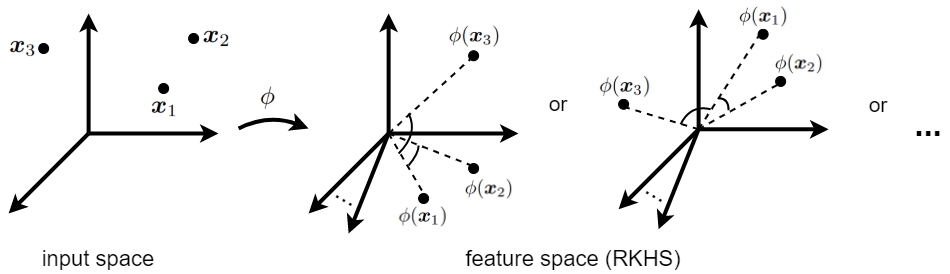
\includegraphics[width=6in]{./images/pulling}
\caption{Pulling data from the input space to the feature space (RKHS). The explicit locations of pulled points are not necessarily known but the relative similarity (inner product) of pulled data points is known in the feature space.}
\label{figure_pulling}
\end{figure*}

\section{Characteristics of Kernels}\label{section_kernel_characteristics}

In this section, we review some of the characteristics of kernels including the symmetry and positive semi-definiteness properties of Mercer kernel (recall Definition \ref{definition_Mercer_kernel}).

\begin{lemma}[Symmetry of Kernel]\label{lemma_kernel_is_symmetric}
A square Mercer kernel matrix is symmetric, so we have:
\begin{align}
&\langle f, g \rangle_k = \langle g, f \rangle_k, \quad \text{ or } \label{equation_symmetric_inner_product}\\
&\boldsymbol{K} \in \mathbb{S}^n, \quad \text{i.e.,} \quad k(\boldsymbol{x}, \boldsymbol{y}) = k(\boldsymbol{y}, \boldsymbol{x}).
\end{align}
\end{lemma}
\begin{proof}
\begin{align*}
k(\boldsymbol{x}, \boldsymbol{y}) &\overset{(\ref{equation_kernel_inner_product})}{=} \big\langle \boldsymbol{\phi}(\boldsymbol{x}), \boldsymbol{\phi}(\boldsymbol{y}) \big\rangle_k = \boldsymbol{\phi}(\boldsymbol{x})^\top \boldsymbol{\phi}(\boldsymbol{y}) \\
&\overset{(a)}{=} \boldsymbol{\phi}(\boldsymbol{y})^\top \boldsymbol{\phi}(\boldsymbol{x}) = k(\boldsymbol{y}, \boldsymbol{x}), 
\end{align*}
where $(a)$ is because $\boldsymbol{\phi}(\boldsymbol{x})^\top \boldsymbol{\phi}(\boldsymbol{y})$ and $\boldsymbol{\phi}(\boldsymbol{y})^\top \boldsymbol{\phi}(\boldsymbol{x})$ are scalars and are equivalent according to the definition of dot product between vectors. Q.E.D.
\end{proof}

\begin{lemma}[Zero Kernel]
We have:
\begin{align}
\langle f, f \rangle_k = 0 \quad \text{iff} \quad f = 0.
\end{align}
\end{lemma}
\begin{proof}
\begin{align*}
0 &\leq f^2(\boldsymbol{x}) \overset{(\ref{equation_RKHS_reproducing})}{=} \langle f, k_{\boldsymbol{x}} \rangle_k\,\, \langle f, k_{\boldsymbol{x}} \rangle_k \\
&\overset{(a)}{\leq} \|f\|_k \|k_{\boldsymbol{x}}\|_k \,\, \|f\|_k \|k_{\boldsymbol{x}}\|_k = \|f\|_k^2\, \|k_{\boldsymbol{x}}\|_k^2 \overset{(b)}{=} 0,
\end{align*}
where $(a)$ is because Cauchy-Schwarz inequality and $(b)$ is because we had assumed $\langle f, f \rangle_k = \|f\|_k = 0$. Hence:
\begin{align*}
0 \leq f^2(\boldsymbol{x}) = 0 \implies f(\boldsymbol{x}) = 0.
\end{align*}
\end{proof}


\begin{lemma}[Positive Semi-definiteness of Kernel]\label{lemma_kernel_is_positive_semidefinite}
The Mercer kernel matrix is positive semi-definite:
\begin{align}
\boldsymbol{K} \in \mathbb{S}_{+}^n, \quad \text{i.e.,} \quad \boldsymbol{K} \succeq \boldsymbol{0}.
\end{align}
\end{lemma}
\begin{proof}
Let $\boldsymbol{v}(i)$ denote the $i$-th element of vector $\boldsymbol{v}$.
\begin{align*}
\boldsymbol{v}^\top \boldsymbol{K} \boldsymbol{v} &\overset{(\ref{equation_Gram_matrix})}{=} \sum_{i=1}^n \sum_{j=1}^n \boldsymbol{v}(i)\, \boldsymbol{v}(j)\, k(\boldsymbol{x}(i), \boldsymbol{x}(j)) \\
&\overset{(\ref{equation_RKHS_inner_product})}{=} \sum_{i=1}^n \sum_{j=1}^n \boldsymbol{v}(i)\, \boldsymbol{v}(j)\, \Big\langle \boldsymbol{\phi}\big(\boldsymbol{x}(i)\big), \boldsymbol{\phi}\big(\boldsymbol{x}(j)\big) \Big\rangle_k \\
&= \sum_{i=1}^n \sum_{j=1}^n \Big\langle \boldsymbol{v}(i)\, \boldsymbol{\phi}\big(\boldsymbol{x}(i)\big), \boldsymbol{v}(j)\, \boldsymbol{\phi}\big(\boldsymbol{x}(j)\big) \Big\rangle_k \\
&= \Big\langle \sum_{i=1}^n \boldsymbol{v}(i)\, \boldsymbol{\phi}\big(\boldsymbol{x}(i)\big), \sum_{j=1}^n \boldsymbol{v}(j)\, \boldsymbol{\phi}\big(\boldsymbol{x}(j)\big) \Big\rangle_k \\
&= \Big\| \sum_{i=1}^n \boldsymbol{v}(i)\, \boldsymbol{\phi}\big(\boldsymbol{x}(i)\big) \Big\|_k^2 \geq 0, \quad \forall \boldsymbol{v} \in \mathbb{R}^n. 
\end{align*}
Hence, according to the definition of positive semi-definiteness \cite{bhatia2009positive}, we have $\boldsymbol{K} \succeq \boldsymbol{0}$. Q.E.D.
\end{proof}
% https://en.wikipedia.org/wiki/Gram_matrix


\section{Well-known Kernel Functions}\label{section_well_known_kernels}

\subsection{Frequently Used Kernels}

% https://scikit-learn.org/stable/modules/metrics.html#laplacian-kernel
% https://scikit-learn.org/stable/modules/classes.html#module-sklearn.metrics.pairwise

There exist many different kernel functions which are widely used in machine learning \cite{rojo2018digital}. In the following, we list some of the most well-known kernels. 

\textbf{-- Linear Kernel:}

Linear kernel is the simplest kernel which is the inner product of points:
\begin{align}\label{equation_linear_kernel}
k(\boldsymbol{x}, \boldsymbol{y}) := \boldsymbol{x}^\top \boldsymbol{y}.
\end{align}
Comparing this with Eq. (\ref{equation_kernel_inner_product}) shows that in linear kernel we have $\boldsymbol{\phi}(\boldsymbol{x}) = \boldsymbol{x}$. Hence, in this kernel, the feature map is explicitly known. Note that $\boldsymbol{\phi}(\boldsymbol{x}) = \boldsymbol{x}$ shows that data are not pulled to any other space in linear kernel but in the input space, the inner products of points are calculated to obtain the feature space. 
Moreover, recall Remark \ref{remark_linear_kernel_equivalent_to_non_kernelized} which states that, depending on the kernelization approach, using linear kernel may or may not be equivalent to non-kernelized method. 

\textbf{-- Radial Basis Function (RBF) or Gaussian Kernel:}

RBF kernel has a scaled Gaussian (or normal) distribution where the normalization factor of distribution is usually ignored. Hence, it is also called the Gaussian kernel. The RBF kernel is formulated as:
\begin{align}\label{equation_RBF_kernel}
k(\boldsymbol{x}, \boldsymbol{y}) := \exp(-\gamma\, \|\boldsymbol{x} - \boldsymbol{y}\|_2^2) = \exp(-\frac{\|\boldsymbol{x} - \boldsymbol{y}\|_2^2}{\sigma^2}),
\end{align}
where $\gamma := 1/\sigma^2$ and $\sigma^2$ is the variance of kernel. 
A proper value for this parameter is $\gamma=1/d$ where $d$ is the dimensionality of data.
Note that RBF kernel has also been widely used in RBF networks \cite{orr1996introduction} and kernel density estimation \cite{scott1992multivariate}.

\textbf{-- Laplacian Kernel:}

The Laplacian kernel, also called the Laplace kernel, is similar to the RBF kernel but with $\ell_1$ norm rather than squared $\ell_2$ norm. The Laplacian kernel is: 
\begin{align}
k(\boldsymbol{x}, \boldsymbol{y}) := \exp(-\gamma\, \|\boldsymbol{x} - \boldsymbol{y}\|_1) = \exp(-\frac{\|\boldsymbol{x} - \boldsymbol{y}\|_1}{\sigma^2}),
\end{align}
where $\|\boldsymbol{x} - \boldsymbol{y}\|_1$ is also called the Manhattan distance. 
A proper value for this parameter is $\gamma=1/d$ where $d$ is the dimensionality of data.
In some specific fields of science, the Laplacian kernel has been found to perform better than Gaussian kernel \cite{rupp2015machine}. This makes sense because of betting on sparsity principal \cite{hastie2009elements} since $\ell_1$ norm makes algorithm sparse. 
Note that $\ell_2$ norm in RBF kernel is also more sensitive to noise; however, the computation and derivative of $\ell_1$ norm is more difficult than $\ell_2$ norm. 

\textbf{-- Sigmoid Kernel:}

Sigmoid kernel is a hyperbolic tangent function applied on inner product of points. It is formulated as:
\begin{align}
k(\boldsymbol{x}, \boldsymbol{y}) := \tanh(\gamma \boldsymbol{x}^\top \boldsymbol{y} + c),
\end{align}
where $\gamma >0$ is the slope and $c$ is the intercept. Some proper values for these parameters are $\gamma=1/d$ and $c=1$ where $d$ is the dimensionality of data.
Note that the hyperbolic tangent function is also used widely for activation functions in neural networks \cite{goodfellow2016deep}. 

\textbf{-- Polynomial Kernel:}

Polynomial kernel applies a polynomial function with degree $\delta$ (a positive integer) on inner product of points:
\begin{align}
k(\boldsymbol{x}, \boldsymbol{y}) := (\gamma \boldsymbol{x}^\top \boldsymbol{y} + c)^d,
\end{align}
where $\gamma >0$ is the slope and $c$ is the intercept. Some proper values for these parameters are $\gamma=1/d$ and $c=1$ where $d$ is the dimensionality of data.

\textbf{-- Cosine Kernel:}

According to Remark \ref{remark_kernel_is_similarity}, kernel is a measure of similarity and computes the inner product between points in the feature space. 
Cosine kernel computes the similarity between points. It is obtained from the formula of cosine and inner product:
\begin{align}\label{equation_cosine_kernel}
k(\boldsymbol{x}, \boldsymbol{y}) := \cos(\boldsymbol{x}, \boldsymbol{y}) = \frac{\boldsymbol{x}^\top \boldsymbol{y}}{\|\boldsymbol{x}\|_2\, \|\boldsymbol{y}\|_2}.
\end{align}
The normalization in the denominator projects the points onto a unit hyper-sphere so that the inner product measures the similarity of their angles regardless of their lengths. 
Note that angle-based measures such as cosine are found to work better for face recognition compared to Euclidean distances \cite{perlibakas2004distance}.

\textbf{-- Chi-squared Kernel:}

Assume $\boldsymbol{x}(j)$ denotes the $j$-th dimension of the $d$-dimensional point $\boldsymbol{x}$.
The Chi-squared ($\chi^2$) kernel is \cite{zhang2007local}:
\begin{align}
k(\boldsymbol{x}, \boldsymbol{y}) := \exp\Big(\!\!-\!\gamma \sum_{j=1}^d \frac{\big(\boldsymbol{x}(j) - \boldsymbol{y}(j)\big)^2}{\boldsymbol{x}(j) + \boldsymbol{y}(j)}\Big),
\end{align}
where $\gamma >0$ is a parameter (a proper value is $\gamma=1$). 
Note that the summation term inside exponential (without the minus) is the Chi-squared distance which is related to the Chi-squared test in statistics. 

\subsection{Kernel Construction from Distance Metric}

Consider $d_{ij}^2 = ||\boldsymbol{x}_i - \boldsymbol{x}_j||_2^2$ as the squared Euclidean distance between $\boldsymbol{x}_i$ and $\boldsymbol{x}_j$. We have:
\begin{align*}
d_{ij}^2 &= ||\boldsymbol{x}_i - \boldsymbol{x}_j||_2^2 = (\boldsymbol{x}_i - \boldsymbol{x}_j)^\top (\boldsymbol{x}_i - \boldsymbol{x}_j) \\
&= \boldsymbol{x}_i^\top \boldsymbol{x}_i - \boldsymbol{x}_i^\top \boldsymbol{x}_j - \boldsymbol{x}_j^\top \boldsymbol{x}_i + \boldsymbol{x}_j^\top \boldsymbol{x}_j \\
&= \boldsymbol{x}_i^\top \boldsymbol{x}_i - 2\boldsymbol{x}_i^\top \boldsymbol{x}_j + \boldsymbol{x}_j^\top \boldsymbol{x}_j = \boldsymbol{G}_{ii} - 2 \boldsymbol{G}_{ij} + \boldsymbol{G}_{jj},
\end{align*}
where $\mathbb{R}^{n \times n} \ni \boldsymbol{G} := \boldsymbol{X}^\top \boldsymbol{X}$ is the linear Gram matrix. If $\mathbb{R}^n \ni \boldsymbol{g} := [\boldsymbol{g}_1, \dots, \boldsymbol{g}_n] = [\boldsymbol{G}_{11}, \dots, \boldsymbol{G}_{nn}] = \textbf{diag}(\boldsymbol{G})$, we have:
\begin{align*}
& d_{ij}^2 = \boldsymbol{g}_i -2\boldsymbol{G}_{ij} + \boldsymbol{g}_j, \\
& \boldsymbol{D} = \boldsymbol{g}\boldsymbol{1}^\top -2 \boldsymbol{G} +\boldsymbol{1}\boldsymbol{g}^\top = \boldsymbol{1}\boldsymbol{g}^\top -2 \boldsymbol{G} + \boldsymbol{g}\boldsymbol{1}^\top,
\end{align*}
where $\boldsymbol{1}$ is the vector of ones and $\boldsymbol{D}$ is the distance matrix with squared Euclidean distance ($d_{ij}^2$ as its elements). 
Let $\boldsymbol{H}$ denote the centering matrix:
\begin{align}\label{equation_centered_matrix}
\mathbb{R}^{n \times n} \ni \boldsymbol{H} := \boldsymbol{I} - \frac{1}{n} \boldsymbol{1}_n\boldsymbol{1}_n^\top,
\end{align}
and $\boldsymbol{I}$ is the identity matrix, $\boldsymbol{1}_n := [1, \dots, 1]^\top \in \mathbb{R}^n$ and $\boldsymbol{1}_{n \times n} := \boldsymbol{1}_n \boldsymbol{1}_n^\top \in \mathbb{R}^{n \times n}$. 
 We double-center the matrix $\boldsymbol{D}$ as follows \cite{oldford2018lecture}:
\begin{align*}
\boldsymbol{HDH} &= (\boldsymbol{I} - \frac{1}{n}\boldsymbol{1}\boldsymbol{1}^\top) \boldsymbol{D} (\boldsymbol{I} - \frac{1}{n}\boldsymbol{1}\boldsymbol{1}^\top) \\
&= (\boldsymbol{I} - \frac{1}{n}\boldsymbol{1}\boldsymbol{1}^\top) (\boldsymbol{1}\boldsymbol{g}^\top -2 \boldsymbol{G} + \boldsymbol{g}\boldsymbol{1}^\top) (\boldsymbol{I} - \frac{1}{n}\boldsymbol{1}\boldsymbol{1}^\top) \\
&= \big[\underbrace{(\boldsymbol{I} - \frac{1}{n}\boldsymbol{1}\boldsymbol{1}^\top)\boldsymbol{1}}_{=\,\boldsymbol{0}} \boldsymbol{g}^\top -2 (\boldsymbol{I} - \frac{1}{n}\boldsymbol{1}\boldsymbol{1}^\top)\boldsymbol{G}\\ 
&~~~~~ + (\boldsymbol{I} - \frac{1}{n}\boldsymbol{1}\boldsymbol{1}^\top)\boldsymbol{g}\boldsymbol{1}^\top\big] (\boldsymbol{I} - \frac{1}{n}\boldsymbol{1}\boldsymbol{1}^\top) \\
&= -2 (\boldsymbol{I} - \frac{1}{n}\boldsymbol{1}\boldsymbol{1}^\top)\boldsymbol{G}(\boldsymbol{I} - \frac{1}{n}\boldsymbol{1}\boldsymbol{1}^\top) \\
&~~~~~ + (\boldsymbol{I} - \frac{1}{n}\boldsymbol{1}\boldsymbol{1}^\top)\boldsymbol{g}\underbrace{\boldsymbol{1}^\top(\boldsymbol{I} - \frac{1}{n}\boldsymbol{1}\boldsymbol{1}^\top)}_{=\,\boldsymbol{0}} \\
&= -2 (\boldsymbol{I} - \frac{1}{n}\boldsymbol{1}\boldsymbol{1}^\top)\boldsymbol{G}(\boldsymbol{I} - \frac{1}{n}\boldsymbol{1}\boldsymbol{1}^\top) = -2\,\boldsymbol{HGH}.
\end{align*}
\begin{align}\label{equation_linearKernel_and_distanceMAtrix_1}
\therefore~~~~~~~~ \boldsymbol{HGH} = \boldsymbol{H}\boldsymbol{X}^\top\boldsymbol{X}\boldsymbol{H} = -\frac{1}{2} \boldsymbol{HDH}.
\end{align}
Note that $(\boldsymbol{I} - \frac{1}{n}\boldsymbol{1}\boldsymbol{1}^\top)\boldsymbol{1} = \boldsymbol{0}$ and $\boldsymbol{1}^\top(\boldsymbol{I} - \frac{1}{n}\boldsymbol{1}\boldsymbol{1}^\top) = \boldsymbol{0}$ because removing the row mean of $\boldsymbol{1}$ and column mean of of $\boldsymbol{1}^\top$ results in the zero vectors, respectively. 


If data $\boldsymbol{X}$ are already centered, i.e., the mean has been removed ($\boldsymbol{X} \gets \boldsymbol{X}\boldsymbol{H}$), Eq. (\ref{equation_linearKernel_and_distanceMAtrix_1}) becomes:
\begin{align}\label{equation_linearKernel_and_distanceMAtrix_2}
\boldsymbol{X}^\top\boldsymbol{X} = -\frac{1}{2} \boldsymbol{HDH}.
\end{align}

According to the kernel trick, Eq. (\ref{equation_kernel_trick_matrix}), we can write a general kernel matrix rather than the linear Gram matrix in Eq. (\ref{equation_linearKernel_and_distanceMAtrix_2}), to have \cite{cox2008multidimensional}:
\begin{align}\label{equation_generalKernel_and_distanceMAtrix}
\mathbb{R}^{n \times n} \ni \boldsymbol{K} = \boldsymbol{\Phi}(\boldsymbol{X})^\top \boldsymbol{\Phi}(\boldsymbol{X}) = -\frac{1}{2} \boldsymbol{HDH}.
\end{align}
This kernel is double-centered because of $\boldsymbol{HDH}$.  
It is also noteworthy that Eq. (\ref{equation_generalKernel_and_distanceMAtrix}) can be used for unifying the spectral dimensionality reduction methods as special cases of kernel principal component analysis with different kernels. See \cite{ham2004kernel,bengio2004learning} for more details. 

\begin{lemma}[Distance-based Kernel is a Mercer Kernel]
The kernel constructed from a valid distance metric, i.e. Eq. (\ref{equation_generalKernel_and_distanceMAtrix}), is a Mercer kernel. 
\end{lemma}
\begin{proof}
The kernel is symmetric because:
\begin{align*}
\boldsymbol{K}^\top = -\frac{1}{2} \boldsymbol{H}^\top \boldsymbol{D}^\top \boldsymbol{H}^\top \overset{(a)}{=} -\frac{1}{2} \boldsymbol{HDH} = \boldsymbol{K},
\end{align*}
where $(a)$ is because $\boldsymbol{H}$ and $\boldsymbol{D}$ are symmetric matrices. 
Moreover, the kernel is positive semi-definite because:
\begin{align*}
&\boldsymbol{K} = -\frac{1}{2} \boldsymbol{HDH} = \boldsymbol{\Phi}(\boldsymbol{X})^\top \boldsymbol{\Phi}(\boldsymbol{X}) \\
&\implies \boldsymbol{v}^\top \boldsymbol{K} \boldsymbol{v} = \boldsymbol{v}^\top \boldsymbol{\Phi}(\boldsymbol{X})^\top \boldsymbol{\Phi}(\boldsymbol{X}) \boldsymbol{v} \\
&~~~~~~~~~~~~~~~~~~~~~~~ = \|\boldsymbol{\Phi}(\boldsymbol{X}) \boldsymbol{v}\|_2^2 \geq 0, \quad \forall \boldsymbol{v} \in \mathbb{R}^n. 
\end{align*}
Hence, according to Definition \ref{definition_Mercer_kernel}, this kernel is a Mercer kernel. Q.E.D.
\end{proof}

\begin{remark}[Kernel Construction from Metric]
One can use any valid distance metric, satisfying the following properties:
\begin{enumerate}[topsep=0pt,itemsep=-1ex,partopsep=1ex,parsep=1ex]
\item non-negativity: $\boldsymbol{D}(\boldsymbol{x}, \boldsymbol{y}) \geq 0$, 
\item equal points: $\boldsymbol{D}(\boldsymbol{x}, \boldsymbol{y}) = 0 \iff \boldsymbol{x} = \boldsymbol{y}$, 
\item symmetry: $\boldsymbol{D}(\boldsymbol{x}, \boldsymbol{y}) = \boldsymbol{D}(\boldsymbol{y}, \boldsymbol{x})$, 
\item triangular inequality: $\boldsymbol{D}(\boldsymbol{x}, \boldsymbol{y}) \leq \boldsymbol{D}(\boldsymbol{x}, \boldsymbol{z})\! + \boldsymbol{D}(\boldsymbol{z}, \boldsymbol{y})$,
\end{enumerate}
to calculate elements of distance matrix $\boldsymbol{D}$ in Eq. (\ref{equation_linearKernel_and_distanceMAtrix_2}). It is important that the used distance matrix should be a valid distance matrix. Using various distance metrics in Eq. (\ref{equation_linearKernel_and_distanceMAtrix_2}) results in various useful kernels.
\end{remark}

Some examples are the geodesic kernel and Structural Similarity Index (SSIM) kernel, used in Isomap \cite{tenenbaum2000global} and image structure subspace learning \cite{ghojogh2019image}, respectively. 
The geodesic kernel is defined as \cite{tenenbaum2000global,ghojogh2020multidimensional}:
\begin{align}
\boldsymbol{K} = -\frac{1}{2} \boldsymbol{H}\boldsymbol{D}^{(g)}\boldsymbol{H},
\end{align}
where the approximation of geodesic distances using piece-wise Euclidean distances is used in calculating the geodesic distance matrix $\boldsymbol{D}^{(g)}$. 
The SSIM kernel is defined as \cite{ghojogh2019image}:
\begin{align}
\boldsymbol{K} = -\frac{1}{2} \boldsymbol{H} \boldsymbol{D}^{(s)} \boldsymbol{H},
\end{align}
where the distance matrix $\boldsymbol{D}^{(s)}$ is calculated using the SSIM distance \cite{brunet2011mathematical}. 


\subsection{Important Classes of Kernels}\label{section_universal_characteristic_kernels}

In the following, we introduce some of the important classes of kernels which are widely used in statistics and machine learning. A good survey on the classes of kernels is \cite{genton2001classes}.

% search "characteristic" in all this paper:
% \cite{simon2020metrizing}
% \cite{simon2018kernel}

\subsubsection{Bounded Kernels}

\begin{definition}[Bounded Kernel]
A kernel function $k$ is bounded if:
\begin{align}
\sup_{\boldsymbol{x}, \boldsymbol{y} \in \mathcal{X}} k(\boldsymbol{x}, \boldsymbol{y}) < \infty, 
\end{align}
where $\mathcal{X}$ is the input space. Likewise, the kernel matrix $\boldsymbol{K}$ is bounded if $\sup_{\boldsymbol{x}, \boldsymbol{y} \in \mathcal{X}} \boldsymbol{K}(\boldsymbol{x}, \boldsymbol{y}) < \infty$.
\end{definition}

\subsubsection{Integrally Positive Definite Kernels}\label{section_integrally_positive_definite_kernels}

% http://www.math.iit.edu/~fass/590/notes/Notes590_Ch2Print.pdf
\begin{definition}[Integrally Positive Definite Kernel]
A kernel matrix $\boldsymbol{K}$ is integrally positive definite ($\int$ p.d.) on $\Omega \times \Omega$ if:
\begin{align}
\int_\Omega \int_\Omega \boldsymbol{K}(\boldsymbol{x}, \boldsymbol{y}) f(\boldsymbol{x}) f(\boldsymbol{y}) \geq 0, \quad \forall f \in L_2(\Omega).
\end{align}
A kernel matrix $\boldsymbol{K}$ is integrally strictly positive definite ($\int$ s.p.d.) on $\Omega \times \Omega$ if:
\begin{align}
\int_\Omega \int_\Omega \boldsymbol{K}(\boldsymbol{x}, \boldsymbol{y}) f(\boldsymbol{x}) f(\boldsymbol{y}) > 0, \quad \forall f \in L_2(\Omega).
\end{align}
\end{definition}



\subsubsection{Universal Kernels}\label{section_universal_kernels}

% see almost at the end of this video:
% https://www.youtube.com/watch?v=EoM_DF3VAO8

\begin{definition}[Universal Kernel]
Let $C(\mathcal{X})$ denote the space of all continuous functions on space $\mathcal{X}$. A continuous kernel $k$ on a compact metric space $\mathcal{X}$ is called universal if the RKHS $\mathcal{H}$, with kernel function $k$, is dense in $C(\mathcal{X})$. In other words, for every function $g \in C(\mathcal{X})$ and all $\epsilon > 0$, there exists a function $f \in \mathcal{H}$ such that $\|f - g\|_\infty \leq \epsilon$.
\end{definition}

\begin{remark}
We can approximate any function, including continuous functions and functions which can be approximated by continuous functions, using a universal kernel. 
\end{remark}

\begin{lemma}
Consider a function $f : (-r, r) \rightarrow \mathbb{R}$ where $0 < r \leq \infty$ and $f \in C^\infty$ ($C^\infty$ denotes the differentiable space for all degrees of differentiation). Let $\mathcal{X} := \{\boldsymbol{x} \in \mathbb{R}^d\, |\, \|\boldsymbol{x}\|_2 < \sqrt{r}\}$. If the function $f$ can be expanded by Taylor expansion in $0$ as:
\begin{align}
f(\boldsymbol{x}) = \sum_{j=0}^\infty a_j\, \boldsymbol{x}^j, \quad \forall \boldsymbol{x} \in (-r, r),
\end{align}
and $a_j > 0$ for all $j \geq 0$, then $k(\boldsymbol{x}, \boldsymbol{y}) = f(\langle \boldsymbol{x}, \boldsymbol{y} \rangle)$ is a universal kernel on every compact subset of $\mathcal{X}$. 
\end{lemma}
\begin{proof}
Note that the Stone-Weierstrass theorem \cite{de1959stone} is used for the proof of this lemma.
\end{proof}
An example for universal kernel is RBF kernel because its Taylor series expansion is:
\begin{align*}
\exp(-\gamma r) \approx 1 - \gamma r + \frac{\gamma^2}{2} r^2 - \frac{\gamma^3}{6} r^3 + \dots,
\end{align*}
where $r := \|\boldsymbol{x} - \boldsymbol{y}\|_2^2$.
Considering Eq. (\ref{equation_kernel_inner_product}) and noticing that this Taylor series expansion has infinite number of terms, we see that the RKHS for RBF kernel is infinite dimensional because $\phi(\boldsymbol{x})$, although cannot be calculated explicitely for this kernel, will have infinite dimensions. 
Another example for universal kernel is the SSIM kernel \cite{ghojogh2020theoretical}, denoted by $\boldsymbol{K}_s$, whose Taylor series expansion is \cite{ghojogh2019image}:
\begin{align*}
\boldsymbol{K}_s \approx -\frac{5}{16} - \frac{15}{16} r + \frac{5}{16} r^2 - \frac{1}{16} r^3 + \dots,
\end{align*}
where $r$ is the squared SSIM distance \cite{brunet2011mathematical} between images. 
Note that polynomial kernels are not universal. %---> https://www.youtube.com/watch?v=EoM_DF3VAO8
Universal kernels have been widely used for kernel SVM. 
More detailed discussion and proofs for use of universal kernels in kernel SVM can be found in \cite{steinwart2008support}.


\begin{lemma}[\cite{borgwardt2006integrating}]
A kernel is universal if for arbitrary sets of distinct points, it induces strictly positive definite kernel matrices \cite{borgwardt2006integrating,song2008learning}. Conversely, if a kernel matrix can be written as $\boldsymbol{K} = \boldsymbol{K}' + \epsilon \boldsymbol{I}$ where $\boldsymbol{K}' \succeq \boldsymbol{0}$, $\epsilon > 0$, and $\boldsymbol{I}$ is the identity matrix, the kernel function corresponding to $\boldsymbol{K}$ is universal \cite{pan2008transfer}.
\end{lemma}



\subsubsection{Stationary Kernels}

% see page 2, column 2, par 2 in \cite{williams2000effect}

% google it: stationary kernel
% https://george.readthedocs.io/en/latest/user/kernels/

% see its Eq 13 in \cite{noack2021advanced}
\begin{definition}[Stationary Kernel \cite{genton2001classes,noack2021advanced}]
A kernel $k$ is stationary if it is a positive definite function of the form:
\begin{align}\label{equation_stationary_kernel}
k(\boldsymbol{x}, \boldsymbol{y}) = k(\|\boldsymbol{x} - \boldsymbol{y}\|),
\end{align}
where $\|.\|$ is some norm defined on the input space. 
\end{definition}
An example for stationary kernel is the RBF kernel defined in Eq. (\ref{equation_RBF_kernel}) which has the form of Eq. (\ref{equation_stationary_kernel}). 
Stationary kernels are used for Gaussian processes \cite{noack2021advanced}. 

\subsubsection{Characteristic Kernels}

The characteristic kernels, which are widely used for distribution embedding in the Hilbert space, will be defined and explained in Section \ref{section_kernel_embedding_distributions}.
Examples for characteristic kernels are RBF and Laplacian kernels. Polynomial kernels. however, are not characteristic.
Note that the relation between universal kernels, characteristic kernels, and integrally strictly positive definite kernels has been studied in \cite{sriperumbudur2011universality}.








\section{Kernel Centering and Normalization}\label{section_kernel_centering_normalization}

\subsection{Kernel Centering}\label{section_kernel_centering}

In some cases, there is a need to center the pulled data in the feature space. For this, the kernel matrix should be centered in a way that the mean of pulled dataset becomes zero. Note that this will restrict the place of pulled points in the feature space further (see Fig. \ref{figure_centered_pulled_data}); however, because of different possible rotations of pulled points around origin, the exact positions of pulled points are still unknown. 

\begin{figure}[!t]
\centering
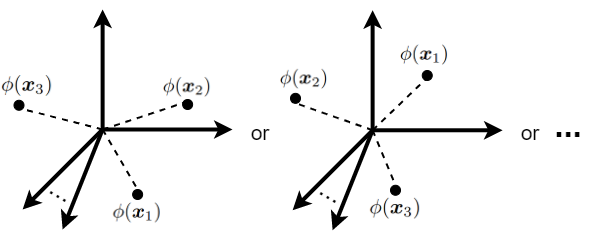
\includegraphics[width=3.4in]{./images/centered_pulled_data}
\caption{Centered pulled data the feature space (RKHS). This happens after kernel centering where the mean of cloud of pulled data becomes zero in RKHS. Even by kernel centering, the explicit locations of pulled points are not necessarily known because of not knowing the rotation of pulled data in that space.}
\label{figure_centered_pulled_data}
\end{figure}

For kernel centering, one should follow the following theory, which is based on \cite{scholkopf1997kernel}. An example of use of kernel centering in machine learning is kernel principal component analysis (see \cite{ghojogh2019unsupervised} for more details). 


\subsubsection{Centering the Kernel of Training Data}

Assume we have some training data $\boldsymbol{X} = [\boldsymbol{x}_1, \dots, \boldsymbol{x}_n] \in \mathbb{R}^{d \times n}$ and some out-of-sample data $\boldsymbol{X}_t = [\boldsymbol{x}_{t,1}, \dots, \boldsymbol{x}_{t,n_t}] \in \mathbb{R}^{d \times n_t}$. 
Consider the kernel matrix for the training data $\mathbb{R}^{n \times n} \ni \boldsymbol{K} := \boldsymbol{\Phi}(\boldsymbol{X})^\top \boldsymbol{\Phi}(\boldsymbol{X})$, whose $(i,j)$-th element is $\mathbb{R} \ni \boldsymbol{K}(i,j) = \boldsymbol{\phi}(\boldsymbol{x}_i)^\top \boldsymbol{\phi}(\boldsymbol{x}_j)$. 
We want to center the pulled training data in the feature space:
\begin{align}\label{equation_appendix_centered_pulled_training}
\breve{\boldsymbol{\phi}}(\boldsymbol{x}_i) := \boldsymbol{\phi}(\boldsymbol{x}_i) - \frac{1}{n} \sum_{k=1}^n \boldsymbol{\phi}(\boldsymbol{x}_k).
\end{align}
If we center the pulled training data, the $(i,j)$-th element of kernel matrix becomes:
\begin{align}
&\breve{\boldsymbol{K}}(i,j) := \breve{\boldsymbol{\phi}}(\boldsymbol{x}_i)^\top \breve{\boldsymbol{\phi}}(\boldsymbol{x}_j) \label{equation_centered_kernel_definition} \\
&\overset{(\ref{equation_appendix_centered_pulled_training})}{=}\! \big(\boldsymbol{\phi}(\boldsymbol{x}_i) - \frac{1}{n} \sum_{k_1=1}^n \boldsymbol{\phi}(\boldsymbol{x}_{k_1})\big)^\top \! \big(\boldsymbol{\phi}(\boldsymbol{x}_j) - \frac{1}{n} \sum_{k_2=1}^n \boldsymbol{\phi}(\boldsymbol{x}_{k_2})\big) \nonumber \\
&= \boldsymbol{\phi}(\boldsymbol{x}_i)^\top \boldsymbol{\phi}(\boldsymbol{x}_j) - \frac{1}{n} \sum_{k_1=1}^n \boldsymbol{\phi}(\boldsymbol{x}_{k_1})^\top \boldsymbol{\phi}(\boldsymbol{x}_j) \nonumber \\
&- \frac{1}{n} \sum_{k_2=1}^n \boldsymbol{\phi}(\boldsymbol{x}_i)^\top \boldsymbol{\phi}(\boldsymbol{x}_{k_2}) + \frac{1}{n^2}\! \sum_{k_1=1}^n  \sum_{k_2=1}^n \boldsymbol{\phi}(\boldsymbol{x}_{k_1})^\top \! \boldsymbol{\phi}(\boldsymbol{x}_{k_2}). \nonumber
\end{align}
Writing this in the matrix form gives:
\begin{align}
\mathbb{R}^{n \times n} \ni \breve{\boldsymbol{K}} &= \boldsymbol{K} - \frac{1}{n} \boldsymbol{1}_{n \times n} \boldsymbol{K} - \frac{1}{n} \boldsymbol{K} \boldsymbol{1}_{n \times n} \nonumber \\
&~~~~ + \frac{1}{n^2} \boldsymbol{1}_{n \times n} \boldsymbol{K} \boldsymbol{1}_{n \times n} = \boldsymbol{H} \boldsymbol{K} \boldsymbol{H}, \label{equation_appendix_doubleCentered_training_kernel}
\end{align}
where $\boldsymbol{H}$ is the centering matrix (see Eq. (\ref{equation_centered_matrix})).
The Eq. (\ref{equation_appendix_doubleCentered_training_kernel}) is called the \textit{double-centered kernel}. 
This equation is the kernel matrix when the pulled training data in the feature space are centered. Also, double-centered kernel has zero row-wise and column-wise mean (so its row and column summations are zero). 
Therefore, after this kernel centering, we will have:
\begin{align}
&\frac{1}{n} \sum_{i=1}^n \breve{\boldsymbol{\phi}}(\boldsymbol{x}_i) = \boldsymbol{0}, \\
&\sum_{i=1}^n \sum_{j=1}^n \breve{\boldsymbol{K}}(i,j) = 0. \label{equation_appendix_doubleCentered_training_kernel_sum}
\end{align}

\subsubsection{Centering the Kernel between Training and Out-of-sample Data}

Now, consider the kernel matrix between the training data and the out-of-sample data $\mathbb{R}^{n \times n_t} \ni \boldsymbol{K}_t := \boldsymbol{\Phi}(\boldsymbol{X})^\top \boldsymbol{\Phi}(\boldsymbol{X}_t)$.
whose $(i,j)$-th element is $\mathbb{R} \ni \boldsymbol{K}_t(i,j) = \boldsymbol{\phi}(\boldsymbol{x}_{i})^\top \boldsymbol{\phi}(\boldsymbol{x}_{t,j})$.
We want to center the pulled training data in the feature space, i.e., Eq. (\ref{equation_appendix_centered_pulled_training}). Moreover, the out-of-sample data should be centered using the mean of training (and not out-of-sample) data:
\begin{align}\label{equation_appendix_centered_pulled_outOfSample}
\breve{\boldsymbol{\phi}}(\boldsymbol{x}_{t,i}) := \boldsymbol{\phi}(\boldsymbol{x}_{t,i}) - \frac{1}{n} \sum_{k=1}^n \boldsymbol{\phi}(\boldsymbol{x}_k).
\end{align}
If we center the pulled training and out-of-sample data, the $(i,j)$-th element of kernel matrix becomes:
\begin{align*}
&\breve{\boldsymbol{K}}_t(i,j) := \breve{\boldsymbol{\phi}}(\boldsymbol{x}_i)^\top \breve{\boldsymbol{\phi}}(\boldsymbol{x}_{t,j}) \\
&\overset{(a)}{=} \! \big(\boldsymbol{\phi}(\boldsymbol{x}_i) - \frac{1}{n} \sum_{k_1=1}^n \boldsymbol{\phi}(\boldsymbol{x}_{k_1})\big)^\top \! \big(\boldsymbol{\phi}(\boldsymbol{x}_{t,j}) - \frac{1}{n} \sum_{k_2=1}^n \boldsymbol{\phi}(\boldsymbol{x}_{k_2})\big) \\
&= \boldsymbol{\phi}(\boldsymbol{x}_i)^\top \boldsymbol{\phi}(\boldsymbol{x}_{t,j}) - \frac{1}{n} \sum_{k_1=1}^n \boldsymbol{\phi}(\boldsymbol{x}_{k_1})^\top \boldsymbol{\phi}(\boldsymbol{x}_{t,j}) \\
& - \frac{1}{n} \sum_{k_2=1}^n \boldsymbol{\phi}(\boldsymbol{x}_i)^\top \boldsymbol{\phi}(\boldsymbol{x}_{k_2}) + \frac{1}{n^2} \! \sum_{k_1=1}^n  \sum_{k_2=1}^n \boldsymbol{\phi}(\boldsymbol{x}_{k_1})^\top \! \boldsymbol{\phi}(\boldsymbol{x}_{k_2}),
\end{align*}
where (a) is because of Eqs. (\ref{equation_appendix_centered_pulled_training}) and (\ref{equation_appendix_centered_pulled_outOfSample}).
Therefore, the double-centered kernel matrix over training and out-of-sample data is:
\begin{align}
\mathbb{R}^{n \times n_t} \ni \breve{\boldsymbol{K}}_t &= \boldsymbol{K}_t - \frac{1}{n} \boldsymbol{1}_{n \times n} \boldsymbol{K}_t - \frac{1}{n} \boldsymbol{K} \boldsymbol{1}_{n \times n_t} \nonumber \\
&~~~~ + \frac{1}{n^2} \boldsymbol{1}_{n \times n} \boldsymbol{K} \boldsymbol{1}_{n \times n_t}, \label{equation_appendix_doubleCentered_outOfSample_kernel}
\end{align}
where $\mathbb{R}^{n \times n_t} \ni \boldsymbol{1}_{n \times n_t} := \boldsymbol{1}_n \boldsymbol{1}_{n_t}^\top$ and $\mathbb{R}^{n_t} \ni \boldsymbol{1}_{n_t} := [1, \dots, 1]^\top$.
The Eq. (\ref{equation_appendix_doubleCentered_outOfSample_kernel}) is the kernel matrix when the pulled training data in the feature space are centered and the pulled out-of-sample data are centered using the mean of pulled training data.

If we have one out-of-sample $\boldsymbol{x}_t$, the Eq. (\ref{equation_appendix_doubleCentered_outOfSample_kernel}) becomes:
\begin{align}
\mathbb{R}^{n} \ni \breve{\boldsymbol{k}}_t &= \boldsymbol{k}_t - \frac{1}{n} \boldsymbol{1}_{n \times n} \boldsymbol{k}_t - \frac{1}{n} \boldsymbol{K} \boldsymbol{1}_{n} + \frac{1}{n^2} \boldsymbol{1}_{n \times n} \boldsymbol{K} \boldsymbol{1}_{n}, \label{equation_appendix_doubleCentered_outOfSample_kernel_oneSample}
\end{align}
where:
\begin{align}
&\mathbb{R}^n \ni \boldsymbol{k}_t = \boldsymbol{k}_t(\boldsymbol{X}, \boldsymbol{x}_t) := \boldsymbol{\Phi}(\boldsymbol{X})^\top \boldsymbol{\phi}(\boldsymbol{x}_t) \label{equation_appendix_kernelVector_outOfSample} \\
&~~~~~~~~~~~~~~ =[\boldsymbol{\phi}(\boldsymbol{x}_1)^\top \boldsymbol{\phi}(\boldsymbol{x}_t), \dots, \boldsymbol{\phi}(\boldsymbol{x}_n)^\top \boldsymbol{\phi}(\boldsymbol{x}_t)]^\top, \nonumber \\
&\mathbb{R}^n \ni \breve{\boldsymbol{k}}_t = \breve{\boldsymbol{k}}_t(\boldsymbol{X}, \boldsymbol{x}_t) := \breve{\boldsymbol{\Phi}}(\boldsymbol{X})^\top \breve{\boldsymbol{\phi}}(\boldsymbol{x}_t), \label{equation_appendix_centered_kernelVector_outOfSample} \\
&~~~~~~~~~~~~~~ =[\breve{\boldsymbol{\phi}}(\boldsymbol{x}_1)^\top \breve{\boldsymbol{\phi}}(\boldsymbol{x}_t), \dots, \breve{\boldsymbol{\phi}}(\boldsymbol{x}_n)^\top \breve{\boldsymbol{\phi}}(\boldsymbol{x}_t)]^\top, \nonumber 
\end{align}
where $\breve{\boldsymbol{\Phi}}(\boldsymbol{X})$ and $\breve{\boldsymbol{\phi}}(\boldsymbol{x}_t)$ are according to Eqs. (\ref{equation_appendix_centered_pulled_training}) and (\ref{equation_appendix_centered_pulled_outOfSample}), respectively.

Note that Eq. (\ref{equation_appendix_doubleCentered_training_kernel}) or  (\ref{equation_appendix_doubleCentered_outOfSample_kernel}) can be restated as the following lemma.
\begin{lemma}[Kernel Centering \cite{bengio2003learning,bengio2003spectral}]\label{lemma_kernel_centering}
The pulled data to the feature space can be centered by kernel centering. The kernel matrix $\boldsymbol{K}(\boldsymbol{x},\boldsymbol{y})$ is centered as:
\begin{align}
\breve{\boldsymbol{K}}(\boldsymbol{x},\boldsymbol{y}) &= \big(\boldsymbol{\phi}(\boldsymbol{x}) - \mathbb{E}_x[\boldsymbol{\phi}(\boldsymbol{x})]\big)^\top \big(\boldsymbol{\phi}(\boldsymbol{x}) - \mathbb{E}_x[\boldsymbol{\phi}(\boldsymbol{x})]\big) \nonumber \\
&= \boldsymbol{K}(\boldsymbol{x}, \boldsymbol{y}) - \mathbb{E}_x[\boldsymbol{K}(\boldsymbol{x}, \boldsymbol{y})] - \mathbb{E}_y[\boldsymbol{K}(\boldsymbol{x}, \boldsymbol{y})] \nonumber \\
&~~~ + \mathbb{E}_x[\mathbb{E}_y[\boldsymbol{K}(\boldsymbol{x}, \boldsymbol{y})]]. \label{equation_kernel_centering_with_exptectation}
\end{align}
\end{lemma}
\begin{proof}
The explained derivations for Eqs. (\ref{equation_appendix_centered_pulled_training}) and (\ref{equation_appendix_centered_pulled_outOfSample}) and definition of expectation complete the proof.
\end{proof}
Note that in Eq. (\ref{equation_kernel_centering_with_exptectation}), $\mathbb{E}_x[\boldsymbol{K}(\boldsymbol{x}, \boldsymbol{y})]$, $\mathbb{E}_y[\boldsymbol{K}(\boldsymbol{x}, \boldsymbol{y})]$, and $\mathbb{E}_x[\mathbb{E}_y[\boldsymbol{K}(\boldsymbol{x}, \boldsymbol{y})]]$ are average of rows, average of columns, and total average of rows and columns of the kernel matrix, respectively.

\subsection{Kernel Normalization}

According to Eq. (\ref{equation_kernel_inner_product}), kernel value can be large if the pulled vectors to the feature map have large length. Hence, in practical computations and optimization, it is sometimes required to normalize the kernel matrix. 

\begin{lemma}[Cosine Normalization of Kernel \cite{rennie2005how,ah2010normalized}]
The kernel matrix $\boldsymbol{K} \in \mathbb{R}^{n \times n}$ can be normalized as:
\begin{align}
\boldsymbol{K}(i,j) \gets \frac{\boldsymbol{K}(i,j)}{\sqrt{\boldsymbol{K}(i,i) \boldsymbol{K}(j,j)}}, \quad \forall i,j \in \{1, \dots, n\}.
\end{align}
\end{lemma}
\begin{proof}
Cosine normalizes points onto a unit hyper-sphere and then computes the similarity of points using inner product. Cosine is computed by Eq. (\ref{equation_cosine_kernel}) and according to the relation of norm and inner product, it is:
\begin{align*}
\cos(\boldsymbol{x}_i, \boldsymbol{x}_j) &= \frac{\boldsymbol{x}_i^\top \boldsymbol{x}_j}{\|\boldsymbol{x}_i\|_2\, \|\boldsymbol{x}_j\|_2} = \frac{\boldsymbol{x}_i^\top \boldsymbol{x}_j}{\sqrt{\|\boldsymbol{x}_i\|_2^2\, \|\boldsymbol{x}_j\|_2^2}} \\
&= \frac{\boldsymbol{x}_i^\top \boldsymbol{x}_j}{\sqrt{\boldsymbol{x}_i^\top \boldsymbol{x}_i\, \boldsymbol{x}_j^\top \boldsymbol{x}_j}}.
\end{align*}
According to Remark \ref{remark_kernel_is_similarity}, kernel is also a measure of similarity. 
Using kernel trick, Eq. (\ref{equation_kernel_trick}), the cosine similarity (which is already normalized) is kernelized as:
\begin{align*}
\boldsymbol{K}(i,j) &= \frac{\boldsymbol{\phi}(\boldsymbol{x}_i)^\top \boldsymbol{\phi}(\boldsymbol{x}_j)}{\sqrt{ \boldsymbol{\phi}(\boldsymbol{x}_i)^\top \boldsymbol{\phi}(\boldsymbol{x}_i)\, \boldsymbol{\phi}(\boldsymbol{x}_j)^\top \boldsymbol{\phi}(\boldsymbol{x}_j) }} \\
&\overset{(\ref{equation_kernel_trick})}{=} \frac{\boldsymbol{K}(i,j)}{\sqrt{\boldsymbol{K}(i,i) \boldsymbol{K}(j,j)}}. 
\end{align*}
Q.E.D.
\end{proof}

\begin{definition}[generalized mean with exponent $t$ \cite{ah2010normalized}]
The generalized mean with exponent $t$ as:
\begin{align}\label{equation_generalized_mean}
m_t(a_1, \dots, a_n) := \Big(\frac{1}{p} \sum_{i=1}^p a_i^t\Big)^{\frac{1}{t}}.
\end{align}
The generalized mean becomes the harmonic, geometric, and arithmetic mean for $t=-1$, $t \rightarrow 0$, and $t=1$, respectively.
\end{definition}

\begin{definition}[Generalized Kernel Normalization of order $t$ \cite{ah2010normalized}]
The generalized kernel normalization of order $t>0$ normalizes the kernel $\boldsymbol{K} \in \mathbb{R}^{n \times n}$ as:
\begin{align}
\boldsymbol{K}(i,j) \gets \frac{\boldsymbol{K}(i,j)}{m_t\big(\boldsymbol{K}(i,i), \boldsymbol{K}(j,j)\big)}, \quad \forall i,j \in \{1, \dots, n\}.
\end{align}
\end{definition}

Both cosine normalization and generalized normalization make the kernel of every point with itself one. In other words, after normalization, we have:
\begin{align}
k(\boldsymbol{x}, \boldsymbol{x}) = 1, \quad \forall \boldsymbol{x} \in \mathcal{X}.
\end{align}
As the most similar point to a point is itself, the values of a normalized kernel will be less than or equal to one. In other words, after normalization, we have:
\begin{align}
k(\boldsymbol{x}_i, \boldsymbol{x}_j) \leq 1, \quad \forall i,j \in \{1, \dots, n\}.
\end{align}
This helps the values not explode to large values in algorithms, especially in the iterative algorithms (e.g., algorithms which use gradient descent for optimization). 


\section{Eigenfunctions}\label{section_eigenfunctions}

\subsection{Inner Product in Hilbert Space}

% https://www.youtube.com/watch?v=g-eNeXlZKAQ
\begin{lemma}[Inner Product in Hilbert Space]
If the domain of functions in a Hilbert space $\mathcal{H}$ is $[a,b]$, the inner product of two functions in the Hilbert space is calculated as:
\begin{align}\label{equation_Hilbert_inner_product}
\langle f(x), g(x)  \rangle_\mathcal{H} = \int_a^b f(x)\, g^*(x) dx \!\overset{(\ref{equation_symmetric_inner_product})}{=}\!\! \int_a^b f^*(x)\, g(x) dx,
\end{align}
where $g^*$ is the complex conjugate of function $g$. If functions are real, the inner product is simplified to $\int_a^b f(x)\, g(x) dx$.
\end{lemma}
\begin{proof}
If we discretize the domain $[a,b]$, for example by sampling, with step $\Delta x$, the function values become vectors as $\boldsymbol{f}(x) = [f(x_1), f(x_2), \dots, f(x_n)]^\top$ and $\boldsymbol{g}(x) = [g(x_1), g(x_2), \dots, g(x_n)]^\top$. According to the inner product of two vectors, we have:
\begin{align*}
\langle \boldsymbol{f}(x), \boldsymbol{g}(x)  \rangle = \boldsymbol{g}^H \boldsymbol{f} = \sum_{i=1}^n f(x_i) g(x_i),
\end{align*}
where $g^H$ denotes the conjugate transpose of $g$ (it is transpose if functions are real). Multiplying the sides of this equation by the setp $\Delta x$ gives:
\begin{align*}
\langle \boldsymbol{f}(x), \boldsymbol{g}(x)  \rangle \Delta x = \boldsymbol{g}^H \boldsymbol{f} = \sum_{i=1}^n f(x_i) g(x_i) \Delta x,
\end{align*}
which is a Riemann sum. This is the Riemann approximation of the Eq. (\ref{equation_Hilbert_inner_product}). 
This approximation gets more accurate by $\Delta x \rightarrow 0$ or $n \rightarrow \infty$.
Hence, that equation is a valid inner product in the Hilbert space. Q.E.D.
\end{proof}

\begin{remark}[Interpretation of Inner Product of Functions in Hilbert Space]
The inner product of two functions, i.e. Eq. (\ref{equation_Hilbert_inner_product}), measures how similar two functions are. The more similar they are in their domain $[a,b]$, the larger inner product they have. 
Note that this similarity is more about the pattern (or changes) of functions and not the exact value of functions. If the pattern of functions is very similar, they will have a large inner product. 
\end{remark}

\begin{corollary}[Weighted Inner Product in Hilbert Space \cite{williams2000effect}]
The Eq. (\ref{equation_Hilbert_inner_product}) is the inner product with uniform weighting. With density function $p(x)$, one can weight the inner product in the Hilbert space as (assuming the functions are real):
\begin{align}\label{equation_Hilbert_inner_product_weighted}
\langle f(x), g(x)  \rangle_\mathcal{H} = \int_a^b f(x)\, g(x)\, p(x)\, dx.
\end{align}
\end{corollary}

\subsection{Eigenfunctions}

Recall eigenvalue problem for a matrix $\boldsymbol{A}$ \cite{ghojogh2019eigenvalue}:
\begin{align}
\boldsymbol{A}\, \boldsymbol{\phi}_i = \lambda_i\, \boldsymbol{\phi}_i, \quad \forall i \in \{1, \dots, d\},
\end{align}
where $\boldsymbol{\phi}_i$ and $\lambda_i$ are the $i$-th eigenvector and eigenvalue of $\boldsymbol{A}$, respectively. 
In the following, we introduce the Eigenfunction problem which has a similar form but for an operator rather than a matrix. 

% https://en.wikipedia.org/wiki/Eigenfunction#Link_to_eigenvalues_and_eigenvectors_of_matrices
% https://www.youtube.com/watch?v=-e-ocwZLB9Y
\begin{definition}[Eigenfunction]\label{definition_eigenfunction}
Consider a linear operator $O$ which can be applied on a function $f$. If applying this operator on the function results in a multiplication of function to a constant:
\begin{align}\label{equation_eigenfunction}
O f = \lambda f,
\end{align}
then the function $f$ is an eigenfunction for the operator $O$ and the constant $\lambda$ is the corresponding eigenvalue.
Note that the form of eigenfunction problem is:
\begin{align}
\text{Operator }( \text{function }f ) = \text{constant } \times \text{function }f.
\end{align}
\end{definition}
Some examples of operator are derivative, kernel function, etc. For example, $e^{\lambda x}$ is an eigenfunction of derivative because $\frac{d}{dx} e^{\lambda x} = \lambda e^{\lambda x}$.
Note that eigenfunctions have application in many fields of science including machine learning \cite{bengio2003spectral} and quantum mechanics \cite{reed1972methods}.

Recall that in eigenvalue problem, the eigenvectors show the most important or informative directions of matrix and the corresponding eigenvalue shows the amount of importance \cite{ghojogh2019eigenvalue}. Likewise, in eigenfunction problem of an operator, the eigenfunction is the most important function of the operator and the corresponding eigenvalue shows the amount of this importance. 
This connection between eigenfunction and eigenvalue problems is proved in the following theorem. 

\begin{theorem}[Connection of Eigenfunction and Eigenvalue Problems]\label{theorem_connection_eigenfunction_eigenvalue_problems}
If we assume that the operator and the function are a matrix and a vector, eigenfunction problem is converted to an eigenvalue problem where the vector is the eigenvector of the matrix. 
\end{theorem}
\begin{proof}
Consider any function space such as a Hilbert space. Let $\{\boldsymbol{e}_j\}_{j=1}^n$ be the bases (basis functions) of this function space where $n$ may be infinite. The function $f$ in this space can be represented as a linear combination bases:
\begin{align}\label{equation_proof_eigenfunction_f}
f(\boldsymbol{x}) = \sum_{j=1}^n \alpha_j\, \boldsymbol{e}_j(\boldsymbol{x}).
\end{align}
An example of this linear combination is Eq. (\ref{equation_RKHS}) in RKHS where the bases are kernels. 
Consider the operator $O$ which can be applied on the functions in this function space.
Applying this operator on Eq. (\ref{equation_proof_eigenfunction_f}) gives:
\begin{align}\label{equation_proof_eigenfunction_O_f_1}
O f(\boldsymbol{x}) = O\sum_{j=1}^n \alpha_j\, \boldsymbol{e}_j(\boldsymbol{x}) \overset{(a)}{=} \sum_{j=1}^n \alpha_j\, O\boldsymbol{e}_j(\boldsymbol{x}),
\end{align}
where $(a)$ is because the operator $O$ is a linear operator according to Definition \ref{definition_eigenfunction}.
Also, we have: 
\begin{align}\label{equation_proof_eigenfunction_lambda_f}
O f(\boldsymbol{x}) \overset{(\ref{equation_eigenfunction})}{=} \lambda f(\boldsymbol{x}) \overset{(a)}{=} \sum_{j=1}^n \lambda\, \alpha_j\, \boldsymbol{e}_j(\boldsymbol{x}),
\end{align}
where $(a)$ is because $\lambda$ is a scalar. 

On the other hand, the output function from applying the operator on a function can also be written as a linear combination of the bases:
\begin{align}\label{equation_proof_eigenfunction_O_f_2}
O f(\boldsymbol{x}) = \sum_{j=1}^n \beta_j\, \boldsymbol{e}_j(\boldsymbol{x}).
\end{align}
From Eqs. (\ref{equation_proof_eigenfunction_O_f_1}) and (\ref{equation_proof_eigenfunction_O_f_2}), we have:
\begin{align}\label{equation_proof_eigenfunction_O_f_3}
\sum_{j=1}^n \alpha_j\, O\boldsymbol{e}_j(\boldsymbol{x}) = \sum_{j=1}^n \beta_j\, \boldsymbol{e}_j(\boldsymbol{x}).
\end{align}

In parentheses, consider an $n \times n$ matrix $\boldsymbol{A}$ whose $(i,j)$-th element is the inner product of $\boldsymbol{e}_i$ and $O \boldsymbol{e}_j$:
\begin{align}\label{equation_proof_eigenfunction_A}
\boldsymbol{A}(i,j) := \langle \boldsymbol{e}_i, O\boldsymbol{e}_j \rangle_k \overset{(\ref{equation_Hilbert_inner_product})}{=} \int \boldsymbol{e}_i^*(\boldsymbol{x})\, O\boldsymbol{e}_j(\boldsymbol{x}) d\boldsymbol{x},
\end{align}
where integral is over the domain of functions in the function space. 

Using Eq. (\ref{equation_Hilbert_inner_product}), we take the inner product of sides of Eq. (\ref{equation_proof_eigenfunction_O_f_3}) with an arbitrary basis function $\boldsymbol{e}_i$:
\begin{align*}
\sum_{j=1}^n \alpha_j\, \int \boldsymbol{e}_i^*(\boldsymbol{x})\, O\boldsymbol{e}_j(\boldsymbol{x})\, d\boldsymbol{x} = \sum_{j=1}^n \beta_j\, \int \boldsymbol{e}_i^*(\boldsymbol{x})\, \boldsymbol{e}_j(\boldsymbol{x})\, d\boldsymbol{x}.
\end{align*}
According to Eq. (\ref{equation_proof_eigenfunction_A}), this equation is simplified to:
\begin{align}\label{equation_proof_eigenfunction_sum_alpha_A_beta}
\sum_{j=1}^n \alpha_j\, \boldsymbol{A}(i,j) &= \sum_{j=1}^n \beta_j\, \int \boldsymbol{e}_i^*(\boldsymbol{x})\, \boldsymbol{e}_j(\boldsymbol{x})\, d\boldsymbol{x} \overset{(a)}{=} \beta_i,
\end{align}
which is true for $\forall i \in \{1, \dots n\}$ and $(a)$ is because the bases are orthonormal, so:
\begin{align*}
\langle \boldsymbol{e}_i, \boldsymbol{e}_j \rangle_k \overset{(\ref{equation_Hilbert_inner_product})}{=}
\int \boldsymbol{e}_i^*(\boldsymbol{x})\, \boldsymbol{e}_j(\boldsymbol{x})\, d\boldsymbol{x} =
\left\{
    \begin{array}{ll}
        1 & \mbox{if } i = j, \\
        0 & \mbox{Otherwise.}
    \end{array}
\right.
\end{align*}
The Eq. (\ref{equation_proof_eigenfunction_sum_alpha_A_beta}) can be written in matrix form:
\begin{align}\label{equation_proof_eigenfunction_A_alpha_equals_beta}
\boldsymbol{A} \boldsymbol{\alpha} = \boldsymbol{\beta},
\end{align}
where $\boldsymbol{\alpha} := [\alpha_1, \dots, \alpha_n]^\top$ and $\boldsymbol{\beta} := [\beta_1, \dots, \beta_n]^\top$.

From Eqs. (\ref{equation_proof_eigenfunction_lambda_f}) and (\ref{equation_proof_eigenfunction_O_f_2}), we have:
\begin{align}\label{equation_proof_eigenfunction_lambda_alpha_equals_beta}
\sum_{j=1}^n \lambda\, \alpha_j\, \boldsymbol{e}_j(\boldsymbol{x}) = \sum_{j=1}^n \beta_j\, \boldsymbol{e}_j(\boldsymbol{x}) \implies \lambda\, \boldsymbol{\alpha} = \boldsymbol{\beta}.
\end{align}
Comparing Eqs. (\ref{equation_proof_eigenfunction_A_alpha_equals_beta}) and (\ref{equation_proof_eigenfunction_lambda_alpha_equals_beta}) shows:
\begin{align*}
\boldsymbol{A} \boldsymbol{\alpha} = \lambda\, \boldsymbol{\alpha},
\end{align*}
which is an eigenvalue problem for matrix $\boldsymbol{A}$ with eigenvector $\boldsymbol{\alpha}$ and eigenvalue $\lambda$ \cite{ghojogh2019eigenvalue}. 
Note that, according to Eq. (\ref{equation_proof_eigenfunction_f}), the information of function $f$ is in the coefficients $\alpha_j$'s of the basis functions of space. Therefore, the function is converted to the eigenvector (vector of coefficients) and the operator $O$ is converted to the matrix $\boldsymbol{A}$. Q.E.D.
\end{proof}

\subsection{Use of Eigenfunctions for Spectral Embedding}\label{section_eigenfunctions_for_spectral_embedding}

Consider a Hilbert space $\mathcal{H}$ of functions with the inner product defined by Eq. (\ref{equation_Hilbert_inner_product_weighted}). Let the data in the input space be $\mathcal{X} = \{\boldsymbol{x}_i \in \mathbb{R}^d\}_{i=1}^n$.
In this space, we can consider an operator for the kernel function $K_p$ as \cite{williams2000effect}:
\begin{align}\label{equation_K_operator_integral}
(K_p f)(\boldsymbol{x}) := \int k(\boldsymbol{x},\boldsymbol{y})\, f(\boldsymbol{y})\, p(\boldsymbol{y})\, d\boldsymbol{y},
\end{align}
where $f \in \mathcal{H}$ and the density function $p(\boldsymbol{y})$ can be approximated empirically. 
A discrete approximation of this operator is \cite{williams2000effect}:
\begin{align}\label{equation_discrete_kernel_operator}
(K_{p,n} f)(\boldsymbol{x}) := \frac{1}{n} \sum_{i=1}^n k(\boldsymbol{x},\boldsymbol{x}_i)\, f(\boldsymbol{x}_i),
\end{align}
which converges to Eq. (\ref{equation_K_operator_integral}) if $n \rightarrow \infty$. 

\begin{lemma}[Relation of Eigenvalues of Eigenvalue Problem and Eigenfunction Problem for Kernel]
Assume $\lambda_k$ denotes the $k$-th eigenvalue for eigenfunction decomposition of the operator $K_p$ and $\delta_k$ denotes the $k$-th eigenvalue for eigenvalue problem of the matrix $\boldsymbol{K} \in \mathbb{R}^{n \times n}$. We have:
\begin{align}\label{equation_connection_eigenvalues_for_kernel_operator}
\delta_k = n\, \lambda_k.
\end{align}
\end{lemma}
\begin{proof}
According to Eq. (\ref{equation_eigenfunction}), the eigenfunction problems for the operators $K_p$ and $K_{p,n}$ (discrete version) are:
\begin{equation}\label{equation_eigenfunction_for_discrete_kernel_operator}
\begin{aligned}
&(K_p f_k)(\boldsymbol{x}) = \lambda_k f_k(\boldsymbol{x}), \quad \forall k \in \{1, \dots, n\}, \\
&(K_{p,n} f_k)(\boldsymbol{x}) = \lambda_k f_k(\boldsymbol{x}), \quad \forall k \in \{1, \dots, n\}, 
\end{aligned}
\end{equation}
where $f_k(.)$ is the $k$-th eigenfunction and $\lambda_k$ is the corresponding eigenvalue.
Consider the kernel matrix defined by Definition \ref{definition_Gram_matrix}.
The eigenvalue problem for the kernel matrix is \cite{ghojogh2019eigenvalue}: 
\begin{align}\label{equation_eigenvalue_problem_kernel_operator}
\boldsymbol{K} \boldsymbol{v}_k = \delta_k \boldsymbol{v}_k, \quad \forall k \in \{1, \dots, n\},
\end{align}
where $\boldsymbol{v}_k$ is the $k$-th eigenvector and $\delta_k$ is the corresponding eigenvalue. 
According to Eqs. (\ref{equation_discrete_kernel_operator}) and (\ref{equation_eigenfunction_for_discrete_kernel_operator}), we have:
\begin{align*}
\frac{1}{n} \sum_{i=1}^n k(\boldsymbol{x},\boldsymbol{x}_i)\, f(\boldsymbol{x}_i) = \lambda_k f_k(\boldsymbol{x}), \quad \forall k \in \{1, \dots, n\}.
\end{align*}
When this equation is evaluated only at $\boldsymbol{x}_i \in \mathcal{X}$, we have:
\begin{align*}
&\frac{1}{n} \boldsymbol{K} f_k = \lambda_k f_k, \quad \forall k \in \{1, \dots, n\}, \\
&\implies \boldsymbol{K} f_k = n \lambda_k f_k.
\end{align*}
According to Theorem \ref{theorem_connection_eigenfunction_eigenvalue_problems}, eigenfunction can be seen as an eigenvector. If so, we can say:
\begin{align}\label{equation_eigenvalue_problem_kernel_operator_2}
\boldsymbol{K} f_k = n \lambda_k f_k \implies \boldsymbol{K} \boldsymbol{v}_k = n \lambda_k \boldsymbol{v}_k,
\end{align}
Comparing Eqs. (\ref{equation_eigenvalue_problem_kernel_operator}) and (\ref{equation_eigenvalue_problem_kernel_operator_2}) results in Eq. (\ref{equation_connection_eigenvalues_for_kernel_operator}). Q.E.D.
\end{proof}

\begin{lemma}[Relation of Eigenvalues of Kernel and Covariance in the Feature Space \cite{scholkopf1998nonlinear}]
Consider the covariance of pulled data to the feature space:
\begin{align}\label{equation_covariance_in_feature_space}
\boldsymbol{C}_H := \frac{1}{n} \sum_{i=1}^n \breve{\phi}(\boldsymbol{x}_i) \breve{\phi}(\boldsymbol{x}_i)^\top,
\end{align}
where $\breve{\phi}(\boldsymbol{x}_i)$ is the centered pulled data defined by Eq. (\ref{equation_appendix_centered_pulled_outOfSample}).

which is $t \times t$ dimensional where $t$ may be infinite. 
Assume $\eta_k$ denotes the $k$-th eigenvalue $\boldsymbol{C}_H$ and $\delta_k$ denotes the $k$-th eigenvalue of centered kernel $\breve{\boldsymbol{K}}$. We have:
\begin{align}\label{equation_connection_eigenvalues_for_kernel_and_covariance}
\delta_k = n\, \eta_k.
\end{align}
\end{lemma}
\begin{proof}
The eigenvalue problem for this covariance matrix is:
\begin{align*}
\eta_k\, \boldsymbol{u}_k = \boldsymbol{C}_H\, \boldsymbol{u}_k, \quad \forall k \in \{1, \dots, n\},
\end{align*}
where $\boldsymbol{u}_k$ is the $k$-th eigenvector and $\eta_k$ is its corresponding eigenvalue \cite{ghojogh2019eigenvalue}. 
Left multiplying this equation with $\breve{\phi}(\boldsymbol{x}_j)^\top$ gives:
\begin{align}\label{equation_eigenvalue_problem_of_covariance_in_feature_space}
\eta_k\, \breve{\phi}(\boldsymbol{x}_j)^\top \boldsymbol{u}_k = \breve{\phi}(\boldsymbol{x}_j)^\top \boldsymbol{C}_H\, \boldsymbol{u}_k, \quad \forall k \in \{1, \dots, n\}.
\end{align}
As $\boldsymbol{u}_k$ is the eigenvector of the covariance matrix in the feature space, it lies in the feature space; hence, according to Lemma \ref{lemma_representation_function_bases} which will come later, we can represent it as:
\begin{align}\label{equation_eigenvector_of_covariance_in_feature_space}
\boldsymbol{u}_k = \frac{1}{\sqrt{\delta_k}} \sum_{\ell=1}^n v_\ell\, \breve{\phi}(\boldsymbol{x}_\ell), 
\end{align}
where pulled data to feature space are assumed to be centered, $v_\ell$'s are the coefficients in representation, and the normalization by $1/\sqrt{\delta_k}$ is because of a normalization.
Substituting Eq. (\ref{equation_eigenvector_of_covariance_in_feature_space}) and Eq. (\ref{equation_covariance_in_feature_space}) in Eq. (\ref{equation_eigenvalue_problem_of_covariance_in_feature_space}) results in:
\begin{align*}
\eta_k\, \breve{\phi}(\boldsymbol{x}_j)^\top &\sum_{\ell=1}^n v_\ell\, \breve{\phi}(\boldsymbol{x}_\ell) \\
&= \breve{\phi}(\boldsymbol{x}_j)^\top \frac{1}{n} \sum_{i=1}^n \breve{\phi}(\boldsymbol{x}_i) \breve{\phi}(\boldsymbol{x}_i)^\top\, \sum_{\ell=1}^n v_\ell\, \breve{\phi}(\boldsymbol{x}_\ell),
\end{align*}
where normalization factors are simplified from sides. 
In the right-hand side, as the summations are finite, we are allowed to re-arrange them. Re-arranging the terms in this equation gives:
\begin{align*}
&\eta_k \sum_{\ell=1}^n v_\ell\, \breve{\phi}(\boldsymbol{x}_j)^\top \breve{\phi}(\boldsymbol{x}_\ell) \\
&~~~~~~ =\frac{1}{n} \sum_{\ell=1}^n v_\ell\, \Big( \breve{\phi}(\boldsymbol{x}_j)^\top \sum_{i=1}^n \breve{\phi}(\boldsymbol{x}_i) \Big) \Big( \breve{\phi}(\boldsymbol{x}_i)^\top\, \breve{\phi}(\boldsymbol{x}_\ell) \Big).
\end{align*}
Considering Eqs. (\ref{equation_kernel_inner_product_matrix}) and (\ref{equation_centered_kernel_definition}), we can write this equation in matrix form $\eta_k \breve{\boldsymbol{K}} \boldsymbol{v}_k = \frac{1}{n} \breve{\boldsymbol{K}}^2 \boldsymbol{v}_k$ where $\boldsymbol{v}_k := [v_1, \dots, v_n]^\top$. As $\breve{\boldsymbol{K}}$ is positive semi-definite (see Lemma \ref{lemma_kernel_is_positive_semidefinite}), it is often non-singular. For non-zero eigenvalues, we can left multiply this equation to $\breve{\boldsymbol{K}}^{-1}$ to have:
\begin{align*}
n\, \eta_k\, \boldsymbol{v}_k = \breve{\boldsymbol{K}} \boldsymbol{v}_k,
\end{align*}
which is the eigenvalue problem for $\breve{\boldsymbol{K}}$ where $\boldsymbol{v}$ is the eigenvector and $\delta_k = n\, \eta_k$ is the eigenvalue (cf. Eq. (\ref{equation_eigenvalue_problem_kernel_operator})). Q.E.D.
\end{proof}

% \subsubsection{Embedding Using Eigenfunctions}

\begin{lemma}[Relation of Eigenfunctions and Eigenvectors for Kernel] \label{lemma_relation_eigenfunctions_eigenvectors_for_kernel}
Consider a training dataset $\{\boldsymbol{x}_i \in \mathbb{R}^d\}_{i=1}^n$ and the eigenvalue problem (\ref{equation_eigenvalue_problem_kernel_operator}) where $\boldsymbol{v}_k \in \mathbb{R}^n$ and $\delta_k$ are the $k$-th eigenvector and eigenvalue of matrix $\boldsymbol{K} \in \mathbb{R}^{n \times n}$.
If $v_{ki}$ is the $i$-th element of vector $\boldsymbol{v}_k$, the eigenfunction for the point $\boldsymbol{x}$ and the $i$-th training point $\boldsymbol{x}_i$ are:
\begin{align}
&f_k(\boldsymbol{x}) = \frac{\sqrt{n}}{\delta_k} \sum_{i=1}^n v_{ki}\, \breve{k}(\boldsymbol{x}_i, \boldsymbol{x}), \label{equation_relation_eigenfunction_eigenvector_x} \\
&f_k(\boldsymbol{x}_i) = \sqrt{n}\, v_{ki}, \label{equation_relation_eigenfunction_eigenvector_x_i}
\end{align}
respectively, where $\breve{k}(\boldsymbol{x}_i, \boldsymbol{x})$ is the centered kernel. 
If $\boldsymbol{x}$ is a training point, $\breve{k}(\boldsymbol{x}_i, \boldsymbol{x})$ is the centered kernel over training data and if $\boldsymbol{x}$ is an out-of-sample point, then $\breve{k}(\boldsymbol{x}_i, \boldsymbol{x}) = \breve{k}_t(\boldsymbol{x}_i, \boldsymbol{x})$ is between training set and the out-of-sample point (n.b. kernel centering is explained in Section \ref{section_kernel_centering}). 
\end{lemma}

It is noteworthy that Eq. (\ref{equation_relation_eigenfunction_eigenvector_x}) is similar and related to the Nystr{\"o}m approximation of eigenfunctions of kernel operator which will be explained in Lemma \ref{lemma_Nystrom_approx_eigenfunctions}.



\begin{theorem}[Embedding from Eigenfunctions of Kernel Operator]\label{theorem_embedding_from_eigenfunctions}
Consider a dimensionality reduction algorithm which embeds data into a low-dimensional embedding space.
Let the embedding of the point $\boldsymbol{x}$ be $\mathbb{R}^p \ni \boldsymbol{y}(\boldsymbol{x}) = [y_1(\boldsymbol{x}), \dots, y_p(\boldsymbol{x})]^\top$ where $p \leq n$. The $k$-th dimension of this embedding is:
\begin{align}\label{equation_embedding_eigenfunction}
y_k(\boldsymbol{x}) &= \sqrt{\delta_k}\, \frac{f_k(\boldsymbol{x})}{\sqrt{n}} = \frac{1}{\sqrt{\delta_k}} \sum_{i=1}^n v_{ki}\, \breve{k}(\boldsymbol{x}_i, \boldsymbol{x}),
\end{align}
where $\breve{k}(\boldsymbol{x}_i, \boldsymbol{x})$ is the centered training or out-of-sample kernel depending on whether $\boldsymbol{x}$ is a training or an out-of-sample point (n.b. kernel centering will be explained in Section \ref{section_kernel_centering}). 
\end{theorem}
\begin{proof}
We can embed data point $\boldsymbol{x}$ by pulling it to the feature space and centering the pulled dataset to have $\breve{\phi}(\boldsymbol{x})$ and then projecting it onto the eigenvector of covariance matrix in the feature space:
\begin{align*}
y_k(\boldsymbol{x}) &= \boldsymbol{u}_k^\top \breve{\phi}(\boldsymbol{x}) \overset{(\ref{equation_eigenvector_of_covariance_in_feature_space})}{=} \frac{1}{\sqrt{\delta_k}} \sum_{i=1}^n v_i\, \breve{\phi}(\boldsymbol{x}_i)^\top \breve{\phi}(\boldsymbol{x}) \\
&\overset{(\ref{equation_centered_kernel_definition})}{=} \frac{1}{\sqrt{\delta_k}} \sum_{i=1}^n v_{ki}\, \breve{k}(\boldsymbol{x}_i, \boldsymbol{x}).
\end{align*}
Q.E.D.
\end{proof}
The Theorem \ref{theorem_embedding_from_eigenfunctions} has been widely used for out-of-sample (test data) embedding in many spectral dimensionality reduction algorithms \cite{bengio2003out}.

\begin{corollary}[Embedding from Eigenvectors of Kernel Matrix]
Consider the eigenvalue problem for the kernel matrix, i.e. Eq. (\ref{equation_eigenvalue_problem_kernel_operator}), where $\boldsymbol{v}_k = [v_{k1}, \dots, v_{kn}]^\top$ and $\delta_k$ are the $k$-th eigenvector and eigenvalue of kernel, respectively. According to Eqs. (\ref{equation_relation_eigenfunction_eigenvector_x_i}) and (\ref{equation_embedding_eigenfunction}), we can compute the embedding of point $\boldsymbol{x}$, denoted by $\boldsymbol{y}(\boldsymbol{x}) = [y_1(\boldsymbol{x}), \dots, y_p(\boldsymbol{x})]^\top$ (where $p \leq n$) using the eigenvector of kernel as:
\begin{align}\label{equation_embedding_eigenvector_of_kernel}
y_k(\boldsymbol{x}) = \sqrt{\delta_k}\, \frac{1}{\sqrt{n}} (\sqrt{n}) v_{ki} = \sqrt{\delta_k}\, v_{ki}. 
\end{align}
\end{corollary}
The Eq. (\ref{equation_embedding_eigenvector_of_kernel}) is used in several dimensionality reduction methods such as maximum variance unfolding (or semidefinite embedding) \cite{weinberger2005nonlinear,weinberger2006unsupervised,weinberger2006introduction}. We will introduce this method in Section \ref{section_kernel_learning}. 

\section{Kernelization Techniques}\label{section_kernelization_techniques}

Linear algorithms cannot properly handle nonlinear patterns of data obviously. 
When dealing with nonlinear data, if the algorithm is linear, two solutions exist to have acceptable performance:
\begin{enumerate}
\item Either the linear method should be modified to become nonlinear or a completely new nonlinear algorithm should be proposed to be able to handle nonlinear data. Some examples of this category are nonlinear dimensionality methods such as locally linear embedding \cite{ghojogh2020locally} and Isomap \cite{ghojogh2020multidimensional}. 
\item Or the nonlinear data should be modified in a way to become more linear in pattern. In other words, a transformation should be applied on data so that the pattern of data becomes roughly linear or easier to process by the linear algorithm. Some examples of this category are kernel versions of linear methods such as kernel Principal Component Analysis (PCA) \cite{scholkopf1997kernel,scholkopf1998nonlinear,ghojogh2019unsupervised}, kernel Fisher Discriminant Analysis (FDA) \cite{mika1999fisher,ghojogh2019fisher}, and kernel Support Vector Machine (SVM) \cite{boser1992training,vapnik1995nature}. 
\end{enumerate}
The second approach is called kernelization in machine learning which we define in the following. 
Figure \ref{figure_separating_classes_kernel} shows how kernelization for transforming data can help separate classes for better classification. 

\begin{figure}[!t]
\centering
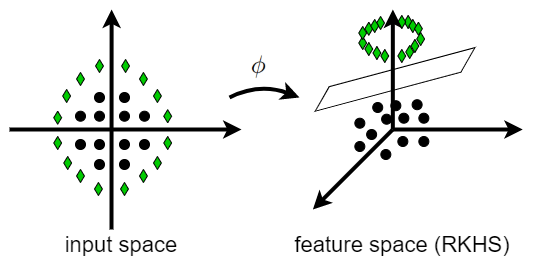
\includegraphics[width=3.4in]{./images/separating_classes}
\caption{Transforming data to RKHS using kernels to make the nonlinear pattern of data more linear. For example, here the classes have become linearly separable (by a linear hyperplane) after kernelization.}
\label{figure_separating_classes_kernel}
\end{figure}

\begin{definition}[Kernelization]
In machine learning and data science, kernelization means a slight change in algorithm formulation (without any modification in the idea of algorithm) so that the pulled data to the RKHS, rather than the raw data, are used as input of algorithm. 
\end{definition}
Note that kernelization can be useful for enabling linear algorithms to handle nonlinear data better. Nevertheless, it should be noted that nonlinear algorithms can also be kernelized to be able to handle nonlinear data perhaps better by transforming data. 

Generally, there exist two main approaches for kernelization in machine learning. These two approaches are related in theory but have two ways for kernelization. 
In the following, we explain these methods which are kernel trick and kernelization using representation theory. 
%This part is based on the experience of authors of this paper by working on machine learning. 

\subsection{Kernelization by Kernel Trick}\label{section_kernel_trick}

Recall Eqs. (\ref{equation_kernel_inner_product}) and (\ref{equation_kernel_inner_product_matrix}) where kernel can be computed by inner product between pulled data instances to the RKHS. 
One technique to kernelize an algorithm is kernel trick. In this technique, we first try to formulate the algorithm formulas or optimization in a way that data always appear as inner product of data instances and not a data instance alone. In other words, the formulation of algorithm should only have $\boldsymbol{x}^\top \boldsymbol{x}$, $\boldsymbol{x}^\top \boldsymbol{X}$, $\boldsymbol{X}^\top \boldsymbol{x}$, or $\boldsymbol{X}^\top \boldsymbol{X}$ and not a lonely $\boldsymbol{x}$ or $\boldsymbol{X}$. In this way, kernel trick replaces $\boldsymbol{x}^\top \boldsymbol{x}$ with $\boldsymbol{\phi}(\boldsymbol{x})^\top \boldsymbol{\phi}(\boldsymbol{x})$ and uses Eq. (\ref{equation_kernel_inner_product}) or (\ref{equation_kernel_inner_product_matrix}). To better explain, kernel trick applies the following mapping \cite{burges1998tutorial}:
\begin{align}\label{equation_kernel_trick}
\boldsymbol{x}^\top \boldsymbol{x} \mapsto \boldsymbol{\phi}(\boldsymbol{x})^\top \boldsymbol{\phi}(\boldsymbol{x}) \overset{(\ref{equation_kernel_inner_product})}{=} k(\boldsymbol{x}, \boldsymbol{x}).
\end{align}
Therefore, the inner products of points are all replaced with the kernel between points. The matrix form of kernel trick is:
\begin{align}\label{equation_kernel_trick_matrix}
\boldsymbol{X}^\top \boldsymbol{X} \mapsto \boldsymbol{\Phi}(\boldsymbol{X})^\top \boldsymbol{\Phi}(\boldsymbol{X}) \overset{(\ref{equation_kernel_inner_product_matrix})}{=} \boldsymbol{K}(\boldsymbol{X}, \boldsymbol{X}) \in \mathbb{R}^{n \times n}.
\end{align}

Most often, kernel matrix is computed over one dataset; hence, its dimensionality is $n \times n$. 
However, in some cases, the kernel matrix is computed between two sets of data instances with sample sizes $n_1$ and $n_2$ for example, i.e. datasets $\boldsymbol{X}_1 := [\boldsymbol{x}_{1,1}, \dots, \boldsymbol{x}_{1,n_1}]$ and $\boldsymbol{X}_2 := [\boldsymbol{x}_{2,1}, \dots, \boldsymbol{x}_{2,n_2}]$. In this case, the kernel matrix has size $n_1 \times n_2$ and the kernel trick is:
\begin{align}
&\boldsymbol{x}_{1,i}^\top \boldsymbol{x}_{1,j} \mapsto \boldsymbol{\phi}(\boldsymbol{x}_{1,i})^\top \boldsymbol{\phi}(\boldsymbol{x}_{1,j}) \overset{(\ref{equation_kernel_inner_product})}{=} k(\boldsymbol{x}_{1,i}, \boldsymbol{x}_{1,j}), \label{equation_kernel_trick_two_sets} \\
&\boldsymbol{X}_1^\top \boldsymbol{X}_2 \mapsto \boldsymbol{\Phi}(\boldsymbol{X}_1)^\top \boldsymbol{\Phi}(\boldsymbol{X}_2) \overset{(\ref{equation_kernel_inner_product_matrix})}{=} \boldsymbol{K}(\boldsymbol{X}_1, \boldsymbol{X}_2) \in \mathbb{R}^{n_1 \times n_2}.
\end{align}
An example for kernel between two sets of data is the kernel between training data and out-of-sample (test) data. 
As stated in \cite{scholkopf2001kernel}, the kernel trick is proved to work for Mercer kernels in \cite{boser1992training,vapnik1995nature} or equivalently for the positive definite kernels \cite{berg1984harmonic,wahba1990spline}.

Some examples of using kernel trick in machine learning are kernel PCA \cite{scholkopf1997kernel,scholkopf1998nonlinear,ghojogh2019unsupervised} and kernel SVM \cite{boser1992training,vapnik1995nature}.
More examples will be provided in Section \ref{section_kernel_in_machine_learning}.
Note that in some algorithms, data do not not appear only by inner product which is required for the kernel trick. In these cases, if possible, a ``dual" method for the algorithm is proposed which only uses the inner product of data. Then, the dual algorithm is kernelized using kernel trick. Some examples for this are kernelization of dual PCA \cite{ghojogh2019unsupervised} and dual SVM \cite{burges1998tutorial}. 
As an additional point, it is noteworthy that it is possible to replace kernel trick with function replacement (see \cite{ma2003function} for more details on this). 


\subsection{Kernelization by Representation Theory}

As was explained in Section \ref{section_kernel_trick}, if the formulation of algorithm has data only as inner products of points, kernel trick can be used. In some cases, a dual version of algorithm is used to have only inner products. 
Some algorithms, however, cannot be formulated in a way to have data only in inner product form, nor does their dual have this form. An example is Fisher Discriminant Analysis (FDA) \cite{ghojogh2019fisher} which uses another technique for kernelization \cite{mika1999fisher}. In the following, we explain this technique. 

\begin{lemma}[Representation of Function Using Bases \cite{mika1999fisher}]\label{lemma_representation_function_bases}
Consider a RKHS denoted by $\mathcal{H}$. Any function $f \in \mathcal{H}$ lies in the span of all points in the RKHS, i.e.,
\begin{align}
f = \sum_{i=1}^n \alpha_i\, \phi(\boldsymbol{x}_i).
\end{align}
\end{lemma}
\begin{proof}
Consider Eq. (\ref{equation_RKHS}) which can be restated as:
\begin{align*}
&f(\boldsymbol{y}) \overset{(\ref{equation_RKHS})}{=} \sum_{i=1}^n \alpha_i\, k(\boldsymbol{x}_i, \boldsymbol{y}) \overset{(\ref{equation_kernel_inner_product})}{=} \sum_{i=1}^n \alpha_i\, \phi(\boldsymbol{x}_i)^\top \phi(\boldsymbol{y}) \\
&\implies f(.) = \sum_{i=1}^n \alpha_i\, \phi(\boldsymbol{x}_i).
\end{align*}
Q.E.D.
\end{proof}

\begin{remark}[Justification by Representation Theory]
According to representation theory \cite{alperin1993local}, any function in the space can be represented as a linear combination of bases of the space. This makes sense because the function is in the space and the space is spanned by the bases. Now, assume the space is RKHS. Hence, any function should lie in the RKHS spanned by the pulled data points to the feature space. This justifies Lemma \ref{lemma_representation_function_bases} using representation theory. 
\end{remark}

\subsubsection{Kernelization for Vector Solution}

Now, consider an algorithm whose optimization variable or solution is the vector/direction $\boldsymbol{u} \in \mathbb{R}^d$ in the input space. 
For kernelization, we pull this solution to RKHS by Eq. (\ref{equation_pulling_mapping}) to have $\phi(\boldsymbol{u})$. 
According to Lemma \ref{lemma_representation_function_bases}, this pulled solution must lie in the span of all pulled training points $\{\phi(\boldsymbol{x}_i)\}_{i=1}^n$ as:
\begin{align}\label{equation_representation_theory_phi_u}
\phi(\boldsymbol{u}) = \sum_{i=1}^n \alpha_i\, \phi(\boldsymbol{x}_i) = \boldsymbol{\Phi}(\boldsymbol{X})\, \boldsymbol{\alpha},
\end{align}
which is $t$ dimensional and $t$ may be infinite. Note that $\boldsymbol{\Phi}(\boldsymbol{X})$ is defined by Eq. (\ref{equation_Phi_X_pulled_matrix}) and is $t \times n$ dimensional. The vector $\boldsymbol{\alpha} := [\alpha_1, \dots, \alpha_n]^\top \in \mathbb{R}^n$ contains the coefficients. 
According to Eq. (\ref{equation_pulling_mapping}), we can replace $\boldsymbol{u}$ with $\phi(\boldsymbol{u})$ in the algorithm. If, by this replacement, the terms $\phi(\boldsymbol{x}_i)^\top \phi(\boldsymbol{x}_i)$ or $\boldsymbol{\Phi}(\boldsymbol{X})^\top \boldsymbol{\Phi}(\boldsymbol{X})$ appear, then we can use Eq. (\ref{equation_kernel_inner_product}) and replace $\phi(\boldsymbol{x}_i)^\top \phi(\boldsymbol{x}_i)$ with $k(\boldsymbol{x}_i, \boldsymbol{x}_i)$ or use Eq. (\ref{equation_kernel_inner_product_matrix}) to replace $\boldsymbol{\Phi}(\boldsymbol{X})^\top \boldsymbol{\Phi}(\boldsymbol{X})$ with $\boldsymbol{K}(\boldsymbol{X}, \boldsymbol{X})$. 
This kernelizes the method. The steps of kernelization by representation theory are summarized below:
\begin{itemize}[topsep=0pt,itemsep=-1ex,partopsep=1ex,parsep=1ex]
\item Step 1: $\boldsymbol{u} \rightarrow \phi(\boldsymbol{u})$
\item Step 2: Replace $\phi(\boldsymbol{u})$ with Eq. (\ref{equation_representation_theory_phi_u}) in the algorithm formulation
\item Step 3: Some $\phi(\boldsymbol{x}_i)^\top \phi(\boldsymbol{x}_i)$ or $\boldsymbol{\Phi}(\boldsymbol{X})^\top \boldsymbol{\Phi}(\boldsymbol{X})$ terms appear in the formulation
\item Step 4: Use Eq. (\ref{equation_kernel_inner_product}) or (\ref{equation_kernel_inner_product_matrix})
\item Step 5: Solve (optimize) the algorithm where the variable to find is $\boldsymbol{\alpha}$ rather than $\boldsymbol{u}$
\end{itemize}
Usually, the goal of algorithm results in kernel. For example, if $\boldsymbol{u}$ is a projection direction, the desired projected data are obtained as:
\begin{align}
\boldsymbol{u}^\top \boldsymbol{x}_i \overset{(\ref{equation_pulling_mapping})}{\mapsto} \phi(\boldsymbol{u})^\top \phi(\boldsymbol{x}_i) &\overset{(\ref{equation_representation_theory_phi_u})}{=} \boldsymbol{\alpha}^\top \boldsymbol{\Phi}(\boldsymbol{X})^\top \phi(\boldsymbol{x}_i) \nonumber \\
&\overset{(\ref{equation_kernel_inner_product_matrix})}{=} \boldsymbol{\alpha}^\top \boldsymbol{k}(\boldsymbol{X}, \boldsymbol{x}_i),
\end{align}
where $\boldsymbol{k}(\boldsymbol{X}, \boldsymbol{x}_i) \in \mathbb{R}^n$ is the kernel between all $n$ training points with the point $\boldsymbol{x}_i$.
As this equation shows, the desired goal is based on kernel. 

\subsubsection{Kernelization for Matrix Solution}

Usually, the algorithm has multiple directions/vectors as its solution. In other words, its solution is a matrix $\boldsymbol{U} = [\boldsymbol{u}_1, \dots, \boldsymbol{u}_p] \in \mathbb{R}^{d \times p}$. In this case, Eq. (\ref{equation_representation_theory_phi_u}) is used for all $p$ vectors and in a matrix form, we have:
\begin{align}\label{equation_representation_theory_phi_u_matrix}
\boldsymbol{\Phi}(\boldsymbol{U}) = \boldsymbol{\Phi}(\boldsymbol{X})\, \boldsymbol{A}, 
\end{align}
where $\mathbb{R}^{n \times p} \ni \boldsymbol{A} := [\boldsymbol{\alpha}_1, \dots, \boldsymbol{\alpha}_p]^\top$ and $\boldsymbol{\Phi}(\boldsymbol{U})$ is $t \times p$ dimensional where $t$ may be infinite. Similarly, the following steps should be performed to kernelize the algorithm:
\begin{itemize}[topsep=0pt,itemsep=-1ex,partopsep=1ex,parsep=1ex]
\item Step 1: $\boldsymbol{U} \rightarrow \phi(\boldsymbol{U})$
\item Step 2: Replace $\phi(\boldsymbol{U})$ with Eq. (\ref{equation_representation_theory_phi_u_matrix}) in the algorithm formulation
\item Step 3: Some $\boldsymbol{\Phi}(\boldsymbol{X})^\top \boldsymbol{\Phi}(\boldsymbol{X})$ terms appear in the formulation
\item Step 4: Use Eq. (\ref{equation_kernel_inner_product_matrix})
\item Step 5: Solve (optimize) the algorithm where the variable to find is $\boldsymbol{A}$ rather than $\boldsymbol{U}$
\end{itemize}
Again the goal of algorithm usually results in kernel. For example, if $\boldsymbol{U}$ is a projection matrix onto its column space, we have:
\begin{align}
\boldsymbol{U}^\top \boldsymbol{x}_i \overset{(\ref{equation_pulling_mapping})}{\mapsto} \phi(\boldsymbol{U})^\top \phi(\boldsymbol{x}_i) &\overset{(\ref{equation_representation_theory_phi_u_matrix})}{=} \boldsymbol{A}^\top \boldsymbol{\Phi}(\boldsymbol{X})^\top \phi(\boldsymbol{x}_i) \nonumber \\
&\overset{(\ref{equation_kernel_inner_product_matrix})}{=} \boldsymbol{A}^\top \boldsymbol{k}(\boldsymbol{X}, \boldsymbol{x}_i),
\end{align}
where $\boldsymbol{k}(\boldsymbol{X}, \boldsymbol{x}_i) \in \mathbb{R}^n$ is the kernel between all $n$ training points with the point $\boldsymbol{x}_i$.
As this equation shows, the desired goal is based on kernel. 

As was mentioned, in many machine learning algorithms, the solution $\boldsymbol{U} \in \mathbb{R}^{d \times p}$ is a projection matrix for projecting $d$-dimensional data onto a $p$-dimensional subspace. Some example methods which have used kernelization by representation theory are kernel Fisher discriminant analysis (FDA) \cite{mika1999fisher,ghojogh2019fisher},
kernel supervised principal component analysis (PCA) \cite{barshan2011supervised,ghojogh2019unsupervised}, and direct kernel Roweis discriminant analysis (RDA) \cite{ghojogh2020generalized}. 

\begin{remark}[Linear Kernel in Kernelization]\label{remark_linear_kernel_equivalent_to_non_kernelized}
If we use kernel trick, the kernelized algorithm with a linear kernel is equivalent to the non-kernelized algorithm. This is because in linear kernel, we have $\phi(\boldsymbol{x}) = \boldsymbol{x}$ and $k(\boldsymbol{x}, \boldsymbol{y}) = \boldsymbol{x}^\top \boldsymbol{y}$ according to Eq. (\ref{equation_linear_kernel}). So, the kernel trick, which is Eq. (\ref{equation_kernel_trick_two_sets}), maps data as $\boldsymbol{x}^\top \boldsymbol{y} \mapsto \phi(\boldsymbol{x})^\top \phi(\boldsymbol{y}) = \boldsymbol{x}^\top \boldsymbol{y}$ for linear kernel. Therefore, linear kernel does not have any effect when using kernel trick. Examples for this are kernel PCA \cite{scholkopf1997kernel,scholkopf1998nonlinear,ghojogh2019unsupervised} and kernel SVM \cite{boser1992training,vapnik1995nature} which are equivalent to PCA and SVM, respectively, if linear kernel is used. 

However, kernel trick does have impact when using kernelization by representation theory because it finds the inner products of pulled data points after pulling the solution and representation as a span of bases. Hence, kernelized algorithm using representation theory with linear kernel is not equivalent to non-kernelized algorithm. Examples of this are kernel FDA \cite{mika1999fisher,ghojogh2019fisher} and kernel supervised PCA \cite{barshan2011supervised,ghojogh2019unsupervised} which are different from FDA and supervised PCA, respectively, even if linear kernel is used. 
\end{remark}







\section{Types of Use of Kernels in Machine Learning}\label{section_kernel_in_machine_learning}

There are several types of using kernels in machine learning. In the following, we explain these types of usage of kernels. 

\subsection{Kernel Methods}

The first type of using kernels in machine learning is kernelization of algorithms using either kernel trick or representation theory. As was discussed in Section \ref{section_kernelization_techniques}, linear methods can be kernelized to handle nonlinear data better. Even nonlinear algorithms can be kernelized to perform in the feature space rather than the input space.
In machine learning both kernel trick and kernelization by representation theory have been used. We provide some examples for each of these categories: 
\begin{itemize}[topsep=0pt,itemsep=-1ex,partopsep=1ex,parsep=1ex]
\item Examples for kernelization by \textbf{kernel trick}: kernel Principal Component Analysis (PCA) \cite{scholkopf1997kernel,scholkopf1998nonlinear,ghojogh2019unsupervised}, kernel Support Vector Machine (SVM) \cite{boser1992training,vapnik1995nature}.
\item Examples for kernelization by \textbf{representation theory}: kernel supervised PCA \cite{barshan2011supervised,ghojogh2019unsupervised}, kernel Fisher Discriminant Analysis (FDA) \cite{mika1999fisher,ghojogh2019fisher}, direct kernel Roweis Discriminant Analysis (RDA) \cite{ghojogh2020generalized}. 
\end{itemize}

As was discussed in Section \ref{section_introduction}, using kernels was widely noticed when linear SVM \cite{vapnik1974theory} was kernelized in \cite{boser1992training,vapnik1995nature}.
More discussions on kernel SVM can be found in \cite{scholkopf1997comparing,hastie2009elements}. A tutorial on kernel SVM is \cite{burges1998tutorial}. 
Universal kernels, introduced in Section \ref{section_universal_characteristic_kernels}, are widely used in kernel SVM. More detailed discussions and proofs for use of universal kernels in kernel SVM can be read in \cite{steinwart2008support}.

As was discussed in Section \ref{section_kernel_trick}, many machine learning algorithms are developed to have dual versions because inner products of points usually appear in the dual algorithms and kernel trick can be applied on them. Some examples of these are dual PCA \cite{scholkopf1997kernel,scholkopf1998nonlinear,ghojogh2019unsupervised} and dual SVM \cite{boser1992training,vapnik1995nature} yielding to kernel PCA and kernel SVM, respectively. 
In some algorithms, however, either a dual version does not exist or formulation does not allow for merely having inner products of points. In those algorithms, kernel trick cannot be used and representation theory should be used. An example for this is FDA \cite{ghojogh2019fisher}.
Moreover, some algorithms, such as kernel reinforcement learning \cite{ormoneit2002kernel}, use kernel as a measure of similarity (see Remark \ref{remark_kernel_is_similarity}).


\subsection{Kernel Learning}\label{section_kernel_learning}

After development of many spectral dimensionality reduction methods in machine learning, it was found out that many of them are actually special cases of kernel Principal Component Analysis (PCA) \cite{bengio2003spectral,bengio2004learning}. 
Paper \cite{ham2004kernel} has shown that PCA, multidimensional scaling, Isomap, locally linear embedding, and Laplacian eigenmap are special cases of kernel PCA with kernels in the formulation of Eq. (\ref{equation_generalKernel_and_distanceMAtrix}).

Because of this, some generalized dimensionality reduction methods, such as graph embedding \cite{yan2005graph}, were proposed.
In addition, as many spectral methods are cases of kernel PCA, some researchers tried to learn the best kernel for manifold unfolding. 
Maximum Variance Unfolding (MVU) or Semidefinite Embedding (SDE) \cite{weinberger2005nonlinear,weinberger2006unsupervised,weinberger2006introduction} is a method for kernel learning using Semidefinite Programming (SDP) \cite{vandenberghe1996semidefinite}. MVU is used for manifold unfolding and dimensionality reduction.
Note that kernel learning by SDP has also been used for labeling a not completely labeled dataset and is also used for kernel SVM \cite{lanckriet2004learning,karimi2017summary}. Our focus here is on MVU. 
In the following, we briefly introduce the MVU (or SDE) algorithm. 

\begin{lemma}[Distance in RKHS \cite{scholkopf2001kernel}]\label{lemma_distance_in_RKHS}
The squared Euclidean distance between points in the feature space is:
\begin{align}\label{equation_distance_in_RKHS}
\|\phi(\boldsymbol{x}_i) - \phi(\boldsymbol{x}_j)\|_k^2 = k(\boldsymbol{x}_i, \boldsymbol{x}_i) + k(\boldsymbol{x}_j, \boldsymbol{x}_j) - 2 k(\boldsymbol{x}_i, \boldsymbol{x}_j).
\end{align}
\end{lemma}
\begin{proof}
\begin{align*}
&\|\phi(\boldsymbol{x}_i) - \phi(\boldsymbol{x}_j)\|_k^2 = \big( \phi(\boldsymbol{x}_i) - \phi(\boldsymbol{x}_j) \big)^\top \big( \phi(\boldsymbol{x}_i) - \phi(\boldsymbol{x}_j) \big) \\
&= \phi(\boldsymbol{x}_i)^\top \phi(\boldsymbol{x}_i) + \phi(\boldsymbol{x}_j)^\top \phi(\boldsymbol{x}_j) -  \phi(\boldsymbol{x}_i)^\top \phi(\boldsymbol{x}_j) \\
&- \phi(\boldsymbol{x}_j)^\top \phi(\boldsymbol{x}_i) \overset{(\ref{equation_symmetric_inner_product})}{=} \phi(\boldsymbol{x}_i)^\top \phi(\boldsymbol{x}_i) + \phi(\boldsymbol{x}_j)^\top \phi(\boldsymbol{x}_j) \\
&- 2\phi(\boldsymbol{x}_i)^\top \phi(\boldsymbol{x}_j) \overset{(\ref{equation_kernel_inner_product})}{=} k(\boldsymbol{x}_i, \boldsymbol{x}_i) + k(\boldsymbol{x}_j, \boldsymbol{x}_j) - 2 k(\boldsymbol{x}_i, \boldsymbol{x}_j).
\end{align*}
Q.E.D.
\end{proof}

MVU desires to unfolds the manifold of data in its maximum variance direction. For example, consider a Swiss roll which can be unrolled to have maximum variance after being unrolled. As trace of matrix is the summation of eigenvalues and kernel matrix is a measure of similarity between points (see Remark \ref{remark_kernel_is_similarity}), the trace of kernel can be used to show the summation of variance of data. Hence, we should maximize $\textbf{tr}(\boldsymbol{K})$ where $\textbf{tr}(.)$ denotes the trace of matrix. 
MVU pulls data to the RKHS and then unfolds the manifold. This unfolding should not ruin the local distances between points after pulling data to the feature space. Hence, we should preserve the local distances as:
\begin{align}
\|\boldsymbol{x}_i - &\boldsymbol{x}_j\|_2^2 \overset{\text{set}}{=} \|\phi(\boldsymbol{x}_i) - \phi(\boldsymbol{x}_j)\|_k^2 \nonumber \\
&\overset{(\ref{equation_distance_in_RKHS})}{=} k(\boldsymbol{x}_i, \boldsymbol{x}_i) + k(\boldsymbol{x}_j, \boldsymbol{x}_j) - 2 k(\boldsymbol{x}_i, \boldsymbol{x}_j).
\end{align}
Moreover, according to Lemma \ref{lemma_kernel_is_positive_semidefinite}, the kernel should be positive semidefinite, i.e. $\boldsymbol{K} \succeq \boldsymbol{0}$. 
MVU also centers kernel to have zero mean for the pulled dataset in the feature space (see Section \ref{section_kernel_centering}). According to Eq. (\ref{equation_appendix_doubleCentered_training_kernel_sum}), we will have $\sum_{i=1}^n \sum_{j=1}^n \boldsymbol{K}(i,j) = 0$. In summary, the optimization of MVU is \cite{weinberger2005nonlinear,weinberger2006unsupervised,weinberger2006introduction}:
\begin{equation}
\begin{aligned}
& \underset{\boldsymbol{K}}{\text{maximize}}
& & \textbf{tr}(\boldsymbol{K}) \\
& \text{subject to}
& & \|\boldsymbol{x}_i - \boldsymbol{x}_j\|_2^2 = \boldsymbol{K}(i,i) + \boldsymbol{K}(j,j) - 2 \boldsymbol{K}(i,j), \\
& & & ~~~~~~~~~~\qquad\qquad\qquad\qquad \; \forall i,j \in \{1, \ldots, n\}, \\
& & & \sum_{i=1}^n \sum_{j=1}^n \boldsymbol{K}(i,j) = 0, \\
& & & \boldsymbol{K} \succeq \boldsymbol{0},
\end{aligned}
\end{equation}
which is a SDP problem \cite{vandenberghe1996semidefinite}. 
Solving this optimization gives the best kernel for maximum variance unfolding of manifold. Then, MVU considers the eigenvalue problem for kernel, i.e. Eq. (\ref{equation_eigenvalue_problem_kernel_operator}), and finds the embedding using Eq. (\ref{equation_embedding_eigenvector_of_kernel}).



\subsection{Use of Kernels for Difference of Distributions}

There exist several different measures for difference of distributions (i.e., PDFs). Some of them make use of kernels and some do not. 
A measure of difference of distributions can be used for (1) calculating the divergence (difference) of a distribution from another reference distribution or (2) convergence of a distribution to another reference distribution using optimization. We will explain the second use of this measure better in Corollary \ref{corollary_characteristic_kernel_convergence_of_distributions}.

For the information of reader, we first enumerate some of the measures without kernels and then introduce the kernel-based measures for difference of distributions. 
One of methods which do not use kernels is the Kullback-Leibler (KL) divergence \cite{kullback1951information}. KL-divergence, which is a relative entropy from one distribution to the other one and has been widely used in deep learning \cite{goodfellow2016deep}.
Another measure is the Wasserstein metric which has been used in generative models \cite{arjovsky2017wasserstein}. 
The integral probability metric \cite{muller1997integral} is another measure for difference of distributions. 
% https://en.wikipedia.org/wiki/Wasserstein_metric

In the following, we introduce some well-known measures for difference of distributions, using kernels. 

\subsubsection{Hilbert-Schmidt Independence Criterion (HSIC)}

Suppose we want to measure the dependence of two random variables. Measuring the correlation between them is easier because correlation is just ``linear'' dependence. 

According to \cite{hein2004kernels}, two random variables $X$ and $Y$ are independent if and only if any bounded continuous functions of them are uncorrelated. Therefore, if we map the samples of two random variables $\{\boldsymbol{x}\}_{i=1}^n$ and $\{\boldsymbol{y}\}_{i=1}^n$ to two different (``separable'') RKHSs and have $\phi(\boldsymbol{x})$ and $\phi(\boldsymbol{y})$, we can measure the correlation of $\phi(\boldsymbol{x})$ and $\phi(\boldsymbol{y})$ in Hilbert space to have an estimation of dependence of $\boldsymbol{x}$ and $\boldsymbol{y}$ in the input space. 

The correlation of $\phi(\boldsymbol{x})$ and $\phi(\boldsymbol{y})$ can be computed by the Hilbert-Schmidt norm of the cross-covariance of them \cite{gretton2005measuring}. Note that the squared Hilbert-Schmidt norm of a matrix $\boldsymbol{A}$ is \cite{bell2016trace}:
\begin{align}
||\boldsymbol{A}||_{HS}^2 := \textbf{tr}(\boldsymbol{A}^\top \boldsymbol{A}),
\end{align}
and the cross-covariance matrix of two vectors $\boldsymbol{x}$ and $\boldsymbol{y}$ is \cite{gubner2006probability,gretton2005measuring}:
\begin{align}
\mathbb{C}\text{ov}(\boldsymbol{x}, \boldsymbol{y}) := \mathbb{E}\Big[&\big(\boldsymbol{x} - \mathbb{E}(\boldsymbol{x})\big) \big(\boldsymbol{y} - \mathbb{E}(\boldsymbol{y})\big) \Big].
\end{align}
Using the explained intuition, an empirical estimation of the Hilbert-Schmidt Independence Criterion (HSIC) is introduced \cite{gretton2005measuring}:
\begin{align}\label{equation_HSIC}
\text{HSIC}(X,Y) := \frac{1}{(n-1)^2}\, \textbf{tr}(\boldsymbol{K}_x\boldsymbol{H}\boldsymbol{K}_y\boldsymbol{H}),
\end{align}
where $\boldsymbol{K}_x := \boldsymbol{\phi}(\boldsymbol{x})^\top \boldsymbol{\phi}(\boldsymbol{x})$ and $\boldsymbol{K}_y := \boldsymbol{\phi}(\boldsymbol{y})^\top \boldsymbol{\phi}(\boldsymbol{y})$ are the kernels over $\boldsymbol{x}$ and $\boldsymbol{y}$, respectively. 
The term $1/(n-1)^2$ is used for normalization.
The matrix $\boldsymbol{H}$ is the centering matrix (see Eq. (\ref{equation_centered_matrix})).
Note that HSIC double-centers one of the kernels and then computes the Hilbert-Schmidt norm between kernels. 

HSIC measures the dependence of two random variable vectors $\boldsymbol{x}$ and $\boldsymbol{y}$. Note that $\text{HSIC}=0$ and $\text{HSIC}>0$ mean that $\boldsymbol{x}$ and $\boldsymbol{y}$ are independent and dependent, respectively. The greater the HSIC, the greater dependence they have.

\begin{lemma}[Independence of Random Variables Using Cross-Covariance]
Two random variables $X$ and $Y$ are independent if and only if $\mathbb{C}\text{ov}(f(\boldsymbol{x}), f(\boldsymbol{y})) = 0$ for any pair of bounded continuous functions $(f,g)$. Because of relation of HSIC with the cross-covariance of variables, two random variables are independent if and only if $\text{HSIC}(X,Y) = 0$.
\end{lemma}

\subsubsection{Maximum Mean Discrepancy (MMD)}

MMD, also known as the kernel two sample test and proposed in \cite{gretton2006kernel,gretton2012kernel}, is a measure for difference of distributions. 
For comparison of two distributions, one can find the difference of all moments of the two distributions. However, as the number of moments is infinite, it is intractable to calculate the difference of all moments. One idea to do this tractably is to pull both distributions to the feature space and then compute the distance of all pulled data points from distributions in RKHS. This difference is a suitable estimate for the difference of all moments in the input space. This is the idea behind MMD. 

MMD is a semi-metric \cite{simon2020metrizing} and uses distance in the RKHS \cite{scholkopf2001kernel} (see Lemma \ref{lemma_distance_in_RKHS}). 
Consider PDFs $\mathbb{P}$ and $\mathbb{Q}$ and samples $\{\boldsymbol{x}_i\}_{i=1}^n \sim \mathbb{P}$ and $\{\boldsymbol{y}_i\}_{i=1}^n \sim \mathbb{Q}$.
The squared MMD between these PDFs is:
\begin{align}
&\text{MMD}^2(\mathbb{P}, \mathbb{Q}) := \Big\|\frac{1}{n} \sum_{i=1}^n \boldsymbol{\phi}(\boldsymbol{x}_i) - \frac{1}{n} \sum_{i=1}^n \boldsymbol{\phi}(\boldsymbol{y}_i)\Big\|_k^2 \nonumber \\
&\overset{(\ref{equation_distance_in_RKHS})}{=} \frac{1}{n^2} \sum_{i=1}^n \sum_{j=1}^n k(\boldsymbol{x}_i, \boldsymbol{x}_j) + \frac{1}{n^2} \sum_{i=1}^n \sum_{j=1}^n k(\boldsymbol{y}_i, \boldsymbol{y}_j) \nonumber \\
&~~~~~~~~~~~~ - \frac{2}{n^2} \sum_{i=1}^n \sum_{j=1}^n k(\boldsymbol{x}_i, \boldsymbol{y}_j) \nonumber \\
&= \mathbb{E}_{x}[\boldsymbol{K}(\boldsymbol{x}, \boldsymbol{y})] + \mathbb{E}_{y}[\boldsymbol{K}(\boldsymbol{x}, \boldsymbol{y})] - 2\mathbb{E}_{x}[\mathbb{E}_{y}[\boldsymbol{K}(\boldsymbol{x}, \boldsymbol{y})]], 
\end{align}
where $\mathbb{E}_x[\boldsymbol{K}(\boldsymbol{x}, \boldsymbol{y})]$, $\mathbb{E}_y[\boldsymbol{K}(\boldsymbol{x}, \boldsymbol{y})]$, and $\mathbb{E}_x[\mathbb{E}_y[\boldsymbol{K}(\boldsymbol{x}, \boldsymbol{y})]]$ are average of rows, average of columns, and total average of rows and columns of the kernel matrix, respectively.
Note that MMD $\geq 0$ where MMD $=0$ means the two distributions are equivalent if the used kernel is characteristic (see Corollary \ref{corollary_characteristic_kernel_convergence_of_distributions} which will be provided later). 
MMD has been widely used in machine learning such as generative moment matching networks \cite{li2015generative}.

\begin{remark}[Equivalence of HSIC and MMD \cite{sejdinovic2013equivalence}]
After development of HSIC and MMD measures, it was found out that they are equivalent.
\end{remark}



\subsection{Kernel Embedding of Distributions (Kernel Mean Embedding)}\label{section_kernel_embedding_distributions}

% https://en.wikipedia.org/wiki/Kernel_embedding_of_distributions

\begin{definition}[Kernel Embedding of Distributions \cite{smola2007hilbert}]
Kernel embedding of distributions, also called the Kernel Mean Embedding (KME) or mean map, represents (or embeds) Probability Density Functions (PDFs) in a RKHS. 
\end{definition}

% https://www.youtube.com/watch?v=uZrEFzEmcng
% https://en.wikipedia.org/wiki/Bochner_integral
\begin{corollary}[Distribution Embedding in Hilbert Space]
Inspired by Eq. (\ref{equation_RKHS}) or (\ref{equation_representer_theorem}), if we map a PDF $\mathbb{P}$ from its space $\mathcal{X}$ to the Hilbert space $\mathcal{H}$, its mapped PDF, denoted by $\phi(\mathbb{P})$, can be represented as:
\begin{align}\label{equation_mapping_PDF_to_RKHS}
\mathbb{P} \mapsto \phi(\mathbb{P}) = \int_\mathcal{X} k(\boldsymbol{x}, .)\, d\mathbb{P}(\boldsymbol{x}).
\end{align}
This integral is called the Bochner integral.
\end{corollary}



KME and MMD were first proposed in the field of pure mathematics \cite{guilbart1978etude}.  
Later on, KME and MMD were used in machine learning, first in \cite{smola2007hilbert}.
KME is a family on methods which use Eq. (\ref{equation_mapping_PDF_to_RKHS}) for embedding PDFs in RKHS. This family of methods is more discussed in \cite{sriperumbudur2010hilbert}. 
A survey on KME is \cite{muandet2016kernel}. 

Universal kernels, introduced in Section \ref{section_universal_kernels}, can be used for KME \cite{sriperumbudur2011universality,simon2018kernel}. In addition to universal kernels, characteristic kernels and integrally strictly positive definite are useful for KME \cite{sriperumbudur2011universality,simon2018kernel}. 
The integrally strictly positive definite kernel was introduced in Section \ref{section_integrally_positive_definite_kernels}. In the following, we introduce the characteristic kernels. 

% https://www.youtube.com/watch?v=uZrEFzEmcng
\begin{definition}[Characteristic Kernel \cite{fukumizu2008characteristic}]\label{definition_characteristic_kernel}
A kernel is characteristic if the mapping (\ref{equation_mapping_PDF_to_RKHS}) is injective. In other words, for a characteristic kernel $k$, we have:
\begin{align}
\mathbb{E}_{X \sim \mathbb{P}}[k(., X)] = \mathbb{E}_{Y \sim \mathbb{Q}}[k(., Y)] \iff \mathbb{P} = \mathbb{Q},
\end{align}
where $\mathbb{P}$ and $\mathbb{Q}$ are two PDFs and $X$ and $Y$ are random variables from these distributions, respectively. 
\end{definition}
Some examples for characteristic kernels are RBF and Laplacian kernels. Polynomial kernels are not characteristic kernels. %%%--> see the middle of video: https://www.youtube.com/watch?v=uZrEFzEmcng

\begin{corollary}[Convergence of Distributions to Each Other Using Characteristic Kernels \cite{simon2020metrizing}]\label{corollary_characteristic_kernel_convergence_of_distributions}
Let $\mathbb{Q}$ be the PDF for a theoretical or sample reference distribution. Following Definition \ref{definition_characteristic_kernel}, if the kernel used in measures for difference of distributions is characteristic, the measure can be used in an optimization framework to converge a PDF $\mathbb{P}$ to the reference distribution $\mathbb{Q}$ as:
\begin{align}
d_k(\mathbb{P}, \mathbb{Q}) = 0 \iff \mathbb{P} = \mathbb{Q}.
\end{align}
where $d_k(.,.)$ denotes a measure for difference of distributions such as MMD. 
\end{corollary}

Characteristic kernels have been used for dimensionality reduction in machine learning. For example, see \cite{fukumizu2004dimensionality,fukumizu2009kernel}.


So far, we have introduced three different types of embedding in RKHS. In the following, we summarize these three types available in the literature of kernels. 
% https://www.youtube.com/watch?v=uZrEFzEmcng
\begin{remark}[Types of Embedding in Hilbert Space]
There are three types of embeddings in Hilbert space:
\begin{enumerate}[topsep=0pt,itemsep=-1ex,partopsep=1ex,parsep=1ex]
\item Embedding of points in the Hilbert space: This embedding maps $\boldsymbol{x} \mapsto k(\boldsymbol{x},.)$ as stated in Sections \ref{section_RKHS} and \ref{section_kernelization_techniques}. 
\item Embedding of functions in the Hilbert space: This embedding maps $f(\boldsymbol{x}) \mapsto \int K(\boldsymbol{x},\boldsymbol{y})\, f(\boldsymbol{y})\, p(\boldsymbol{y})\, d\boldsymbol{y}$ as stated in Section \ref{section_eigenfunctions}.
\item Embedding of distributions (PDF's) in the Hilbert space: This embedding maps $\mathbb{P} \mapsto \int k(\boldsymbol{x}, .)\, d\mathbb{P}(\boldsymbol{x})$ as stated in Section \ref{section_kernel_embedding_distributions}.
\end{enumerate}
Researchers are expecting that a combination of these types of embedding might appear in the future. 
\end{remark}


\subsection{Kernel Dimensionality Reduction for Sufficient Dimensionality Reduction}

Kernels can also be used directly for dimensionality reduction.
Assume $\boldsymbol{X}$ is the random variable of data and $Y$ is the random variables of labels of data. The labels can be discrete finite for classification or continuous for regression. 
Sufficient Dimensionality Reduction (SDR) \cite{adragni2009sufficient} is a family of methods which find a transformation of data to a lower dimensional space, denoted by $R(\boldsymbol{x})$, which does not change the conditional of labels given data:
\begin{align}
\mathbb{P}_{Y | X}(\boldsymbol{y}\, |\, \boldsymbol{x}) = \mathbb{P}_{Y | R(X)}(\boldsymbol{y}\, |\, R(\boldsymbol{x})).
\end{align}

Kernel Dimensionality Reduction (KDR) \cite{fukumizu2004dimensionality,fukumizu2009kernel,wang2010unsupervised} is a SDR method with linear projection for transformation, i.e. $R(\boldsymbol{x}): \boldsymbol{x} \mapsto \boldsymbol{U}^\top \boldsymbol{x}$ which projects data onto the column space of $\boldsymbol{U}$. The goal of KDR is:
\begin{align}
\mathbb{P}_{Y | X}(\boldsymbol{y}\, |\, \boldsymbol{x}) = \mathbb{P}_{Y | U, X}(\boldsymbol{y}\, |\, \boldsymbol{U}, \boldsymbol{x}).
\end{align}

% https://en.wikipedia.org/wiki/Dual_space
\begin{definition}[Dual Space]
A dual space of a vector space $\mathcal{V}$, denoted by $\mathcal{V}^*$, is the set of all linear functionals $\phi: \mathcal{V} \rightarrow \mathcal{F}$ where $\mathcal{F}$ is the field on which vector space is defined. 
\end{definition}

% https://www.youtube.com/watch?v=uZrEFzEmcng
% https://en.wikipedia.org/wiki/Riesz_representation_theorem
\begin{theorem}[Riesz (or Riesz–Fr{\'e}chet) representation theorem \cite{garling1973short}]\label{theorem_Riesz}
Let $\mathcal{H}$ be a Hilbert space with norm $\langle.,.\rangle_\mathcal{H}$. Suppose $\phi \in \mathcal{H}^*$ (e.g., $\phi: f \rightarrow \mathbb{R}$). Then, there exists a unique $f \in \mathcal{H}$ such that for any $\boldsymbol{x} \in \mathcal{H}$, we have $\phi(\boldsymbol{x}) = \langle f,g \rangle$:
\begin{align}
\exists f \in \mathcal{H} : \phi \in \mathcal{H}^*, \forall \boldsymbol{x} \in \mathcal{H}, \quad  \phi(\boldsymbol{x}) = \langle f,\boldsymbol{x} \rangle_\mathcal{H}.
\end{align}
\end{theorem}

% \begin{corollary}
% Let $\mathcal{H}_x$ and $\mathcal{H}_y$ denote the Hilbert spaces corresponding to $X$ and $Y$, respectively. Suppose 
% According to Theorem \ref{theorem_Riesz}, we have:
% \begin{align}
% & \mathbb{E}_X[f(\boldsymbol{x})] = \langle f, \phi_x(\mathbb{P}) \rangle_{\mathcal{H}_x}, \quad \forall f \in \mathcal{H}, \\
% & \mathbb{E}_{Y|X}[g(\boldsymbol{y})\, |\, \boldsymbol{x}] = \langle g, \phi_y(\mathbb{P}) \rangle_{\mathcal{H}_y}, \quad \forall g \in \mathcal{H},
% \end{align}
% \end{corollary}

\begin{corollary}\label{corollary_Riesz_expectation}
According to Theorem \ref{theorem_Riesz}, we have:
\begin{align}
& \mathbb{E}_X[f(\boldsymbol{x})] = \langle f, \phi(\mathbb{P}) \rangle_{\mathcal{H}}, \quad \forall f \in \mathcal{H},
\end{align}
where $\phi(\mathbb{P})$ is defined by Eq. (\ref{equation_mapping_PDF_to_RKHS}).
\end{corollary}

KDR uses Theorem \ref{theorem_Riesz} and Corollary \ref{corollary_Riesz_expectation} in its formualtions. 
Note that characteristic kernels \cite{fukumizu2008characteristic}, introduced in Definition \ref{definition_characteristic_kernel}, are used in KDR. 


\section{Rank and Factorization of Kernel and the Nystr{\"o}m Method}\label{section_factorization_and_Nystrom_method}

\subsection{Rank and Factorization of Kernel Matrix}

Usually, the rank of kernel is small. This is because the manifold hypothesis which states that data points often do not cover the whole space but lie on a sub-manifold. Nystr{\"o}m approximation of the kernel matrix also works well because kernels are often low-rank matrices (we will discuss it in Corollary \ref{corollary_Nystron_rank_discussion}). 
Because of low rank of kernels, they can be approximated \cite{kishore2017literature}, learned \cite{kulis2006learning,kulis2009low}, and factorized. 
Kernel factorization has also be used for the sake of clustering \cite{wang2010low}.
In the following, we introduce some of the most well-known decompositions for the kernel matrix. 

\subsubsection{Singular Value and Eigenvalue Decompositions}

The Singular Value Decomposition (SVD) of the pulled data to the feature space is:
\begin{align}\label{equation_SVD_Phi}
\mathbb{R}^{t \times n} \ni \boldsymbol{\Phi}(\boldsymbol{X}) = \boldsymbol{U}\boldsymbol{\Sigma}\boldsymbol{V}^\top,
\end{align}
where $\boldsymbol{U} \in \mathbb{R}^{t \times n}$ and $\boldsymbol{V} \in \mathbb{R}^{n \times n}$ are orthogonal matrices and contain the left and right singular vectors, respectively, and $\boldsymbol{\Sigma} \in \mathbb{R}^{n \times n}$ is a diagonal matrix with singular values.  
Note that here, we are using notations such as $\mathbb{R}^{t \times n}$ for showing the dimensionality of matrices and this notation does not imply a Euclidean space. 

As mentioned before, the pulled data are not necessarily available so Eq. (\ref{equation_SVD_Phi}) cannot necessarily be done.
The kernel, however, is available.
Using the SVD of pulled data in the formulation of kernel gives:
\begin{align}
&\boldsymbol{K} \overset{(\ref{equation_kernel_inner_product_matrix})}{=} \boldsymbol{\Phi}(\boldsymbol{X})^\top \boldsymbol{\Phi}(\boldsymbol{X}) \overset{(\ref{equation_SVD_Phi})}{=} (\boldsymbol{U}\boldsymbol{\Sigma}\boldsymbol{V}^\top)^\top (\boldsymbol{U}\boldsymbol{\Sigma}\boldsymbol{V}^\top) \nonumber \\
&~~~~~~ = \boldsymbol{V}\boldsymbol{\Sigma}\underbrace{\boldsymbol{U}^\top \boldsymbol{U}}_{=\,\boldsymbol{I}}\boldsymbol{\Sigma}\boldsymbol{V}^\top 
= \boldsymbol{V}\boldsymbol{\Sigma}\boldsymbol{\Sigma}\boldsymbol{V}^\top = \boldsymbol{V}\boldsymbol{\Sigma}^2\boldsymbol{V}^\top, \nonumber \\
&\implies \boldsymbol{K} \boldsymbol{V} = \boldsymbol{V} \boldsymbol{\Sigma}^2 \underbrace{\boldsymbol{V}^\top \boldsymbol{V}}_{=\,\boldsymbol{I}} \implies \boldsymbol{K} \boldsymbol{V} = \boldsymbol{V} \boldsymbol{\Sigma}^2. \label{equation_eigenvalue_problem_kernel_factorization_Sigma2}
\end{align}
If we take $\boldsymbol{\Delta} = \textbf{diag}([\delta_1, \dots, \delta_n]^\top) := \boldsymbol{\Sigma}^2$, this equation becomes:
\begin{align}\label{equation_eigenvalue_problem_kernel_factorization}
\boldsymbol{K} \boldsymbol{V} = \boldsymbol{V} \boldsymbol{\Delta},
\end{align}
which is the matrix of Eq. (\ref{equation_eigenvalue_problem_kernel_operator}), i.e. the eigenvalue problem \cite{ghojogh2019eigenvalue} for the kernel matrix with $\boldsymbol{V}$ and $\boldsymbol{\Delta}$ as eigenvectors and eigenvalues, respectively.
Hence, for SVD on the pulled dataset, one can apply Eigenvalue Decomposition (EVD) on the kernel where the eigenvectors of kernel are equal to right singular vectors of pulled dataset and the eigenvalues of kernel are the squared singular values of pulled dataset. 
This technique has been used in kernel PCA \cite{ghojogh2019unsupervised}. 

\subsubsection{Cholesky and QR Decompositions}

The kernel matrix can be factorized using LU decomposition; however, as the kernel matrix is symmetric positive semi-definite matrix (see Lemmas \ref{lemma_kernel_is_symmetric} and \ref{lemma_kernel_is_positive_semidefinite}), it can be decomposed using Cholesky decomposition which is much faster than LU decomposition. The Cholesky decomposition of kernel is in the form $\mathbb{R}^{n \times n} \ni \boldsymbol{K} = \boldsymbol{L} \boldsymbol{L}^\top$ where $\boldsymbol{L} \in \mathbb{R}^{n \times n}$ is a lower-triangular matrix. 
The kernel matrix can also be factorized using QR decomposition as $\mathbb{R}^{n \times n} \ni \boldsymbol{K} = \boldsymbol{Q} \boldsymbol{R}$ where $\boldsymbol{Q} \in \mathbb{R}^{n \times n}$ is an orthogonal matrix and $\boldsymbol{R} \in \mathbb{R}^{n \times n}$ is an upper-triangular matrix. 
The paper \cite{bach2005predictive} has incorporated side information, such as class labels, in the Cholesky and QR decompositions of kernel matrix. 



\subsection{Nystr{\"o}m Method for Approximation of Eigenfunctions}


Nystr{\"o}m method, first proposed in \cite{nystrom1930praktische}, was initially used for approximating the eigenfunctions of an operator (or of a matrix corresponding to an operator). 
The following lemma provides the Nystr{\"o}m approximation for the eigenfunctions of the kernel operator defined by Eq. (\ref{equation_K_operator_integral}).
For more discussion on this, reader can refer to \cite{baker1977numerical} and \cite{williams2000effect}.

\begin{lemma}[Nystr{\"o}m Approximation of Eigenfunction]\label{lemma_Nystrom_approx_eigenfunctions}
Consider a training dataset $\{\boldsymbol{x}_i \in \mathbb{R}^d\}_{i=1}^n$ and the eigenfunction problem (\ref{equation_eigenfunction}) where $f_k \in \mathcal{H}$ and $\lambda_k$ are the $k$-th eigenfunction and eigenvalue of kernel operator defined by Eq. (\ref{equation_K_operator_integral}) or (\ref{equation_discrete_kernel_operator}).
The eigenfunction can be approximated by Nystr{\"o}m method as:
\begin{align}
&f_k(\boldsymbol{x}) \approx \frac{1}{n \lambda_k} \sum_{i=1}^n k(\boldsymbol{x}_i, \boldsymbol{x})\, f_k(\boldsymbol{x}_i), \label{equation_relation_eigenfunction_eigenvector_x_2} 
\end{align}
where $k(\boldsymbol{x}_i, \boldsymbol{x})$ is the kernel (or centered kernel) corresponding to the kernel operator.  
\end{lemma}
\begin{proof}
This Lemma is somewhat similar and related to Lemma \ref{lemma_relation_eigenfunctions_eigenvectors_for_kernel}. 
Consider the kernel operator, defined by Eq. (\ref{equation_K_operator_integral}), in Eq. (\ref{equation_eigenfunction}): $K f = \lambda f$. Combining this with the discrete version of operator, Eq. (\ref{equation_discrete_kernel_operator}), gives $\lambda_k f_k(\boldsymbol{x}) = (1/n) \sum_{i=1}^n k(\boldsymbol{x}_i, \boldsymbol{x}) f_k(\boldsymbol{x}_i)$
Dividing the sides of this equation by $\lambda_k$ brings Eq. (\ref{equation_relation_eigenfunction_eigenvector_x_2}). Q.E.D.
\end{proof}


\subsection{Nystr{\"o}m Method for Kernel Completion and Approximation}\label{section_Nystrom_for_kernel}

As explained before, the kernel matrix has a low rank often. Because of its low rank, it can be approximated \cite{kishore2017literature}. This is important because in big data when $n \gg 1$, constructing the kernel matrix is both time-consuming and also intractable to store in computer; i.e., its computation will run forever and will raise a memory error finally. Hence, it is desired to compute the kernel function between a subset of data points (called landmarks) and then approximate the rest of kernel matrix using this subset of kernel matrix. Nystr{\"o}m approximation can be used for this goal. 

The Nystr{\"o}m method can be used for kernel approximation. 
It is a technique used to approximate a positive semi-definite matrix using merely a subset of its columns (or rows), \cite{drineas2005nystrom}. 
Hence, it can be used for kernel completion in big data where computation of the entire kernel matrix is time consuming and intractable. One can compute some of the important important columns or rows of a kernel matrix, called landmarks, and approximate the rest of columns or rows by Nystr{\"o}m approximation.

Consider a positive semi-definite matrix $\mathbb{R}^{n \times n} \ni \boldsymbol{K} \succeq 0$ whose parts are:
\begin{align}\label{equation_Nystrom_partions}
\mathbb{R}^{n \times n} \ni \boldsymbol{K} = 
\left[
\begin{array}{c|c}
\boldsymbol{A} & \boldsymbol{B} \\
\hline
\boldsymbol{B}^\top & \boldsymbol{C}
\end{array}
\right],
\end{align}
where $\boldsymbol{A} \in \mathbb{R}^{m \times m}$, $\boldsymbol{B} \in \mathbb{R}^{m \times (n-m)}$, and $\boldsymbol{C} \in \mathbb{R}^{(n-m) \times (n-m)}$ in which $m \ll n$. 
This positive semi-definite matrix can be a kernel (or Gram) matrix. 

The Nystr{\"o}m approximation says if we have the small parts of this matrix, i.e. $\boldsymbol{A}$ and $\boldsymbol{B}$, we can approximate $\boldsymbol{C}$ and thus the whole matrix $\boldsymbol{K}$. The intuition is as follows. Assume $m=2$ (containing two points, a and b) and $n=5$ (containing three other points, c, d, and e). If we know the similarity (or distance) of points a and b from one another, resulting in matrix $\boldsymbol{A}$, as well as the similarity (or distance) of points c, d, and e from a and b, resulting in matrix $\boldsymbol{B}$, we cannot have much freedom on the location of c, d, and e, which is the matrix $\boldsymbol{C}$. This is because of the positive semi-definiteness of the matrix $\boldsymbol{K}$. 
The points selected in submatrix $\boldsymbol{A}$ are named \textit{landmarks}. Note that the landmarks can be selected randomly from the columns/rows of matrix $\boldsymbol{K}$ and, without loss of generality, they can be put together to form a submatrix at the top-left corner of matrix. 
For Nystr{\"o}m approximation, some methods have been proposed for sampling more important columns/rows of matrix more wisely rather than randomly. We will mention some of these sampling methods in Section \ref{section_improvements_over_Nystrom}.

As the matrix $\boldsymbol{K}$ is positive semi-definite, by definition, it can be written as $\boldsymbol{K} = \boldsymbol{O}^\top \boldsymbol{O}$. If we take $\boldsymbol{O} = [\boldsymbol{R}, \boldsymbol{S}]$ where $\boldsymbol{R}$ are the selected columns (landmarks) of $\boldsymbol{O}$ and $\boldsymbol{S}$ are the other columns of $\boldsymbol{O}$. We have:
\begin{align}
\boldsymbol{K} &= \boldsymbol{O}^\top \boldsymbol{O} = 
\begin{bmatrix}
\boldsymbol{R}^\top \\
\boldsymbol{S}^\top
\end{bmatrix}
[\boldsymbol{R}, \boldsymbol{S}] \label{equation_Nystrom_kernel_OtransposeO} \\
&= 
\begin{bmatrix}
\boldsymbol{R}^\top \boldsymbol{R} & \boldsymbol{R}^\top \boldsymbol{S} \\
\boldsymbol{S}^\top \boldsymbol{R} & \boldsymbol{S}^\top \boldsymbol{S}
\end{bmatrix}
\overset{(\ref{equation_Nystrom_partions})}{=} 
\begin{bmatrix}
\boldsymbol{A} & \boldsymbol{B} \\
\boldsymbol{B}^\top & \boldsymbol{C}
\end{bmatrix}.
\end{align}
Hence, we have $\boldsymbol{A} = \boldsymbol{R}^\top \boldsymbol{R}$. The eigenvalue decomposition \cite{ghojogh2019eigenvalue} of $\boldsymbol{A}$ gives:
\begin{align}
&\boldsymbol{A} = \boldsymbol{U} \boldsymbol{\Sigma} \boldsymbol{U}^\top \label{equation_Nystrom_A_eig_decomposition} \\
&\implies \boldsymbol{R}^\top \boldsymbol{R} = \boldsymbol{U} \boldsymbol{\Sigma} \boldsymbol{U}^\top \implies \boldsymbol{R} = \boldsymbol{\Sigma}^{(1/2)} \boldsymbol{U}^\top. \label{equation_Nystrom_R}
\end{align}
Moreover, we have $\boldsymbol{B} = \boldsymbol{R}^\top \boldsymbol{S}$ so we have:
\begin{align}
&\boldsymbol{B} = (\boldsymbol{\Sigma}^{(1/2)} \boldsymbol{U}^\top)^\top \boldsymbol{S} = \boldsymbol{U} \boldsymbol{\Sigma}^{(1/2)} \boldsymbol{S} \nonumber \\
&\overset{(a)}{\implies} \boldsymbol{U}^\top \boldsymbol{B} = \boldsymbol{\Sigma}^{(1/2)} \boldsymbol{S} \implies \boldsymbol{S} = \boldsymbol{\Sigma}^{(-1/2)} \boldsymbol{U}^\top \boldsymbol{B}, \label{equation_Nystrom_S}
\end{align}
where $(a)$ is because $\boldsymbol{U}$ is orthogonal (in the eigenvalue decomposition). 
Finally, we have:
\begin{align}
\boldsymbol{C} &= \boldsymbol{S}^\top \boldsymbol{S} = \boldsymbol{B}^\top \boldsymbol{U} \boldsymbol{\Sigma}^{(-1/2)} \boldsymbol{\Sigma}^{(-1/2)} \boldsymbol{U}^\top \boldsymbol{B} \nonumber \\
&= \boldsymbol{B}^\top \boldsymbol{U} \boldsymbol{\Sigma}^{-1} \boldsymbol{U}^\top \boldsymbol{B} \overset{(\ref{equation_Nystrom_A_eig_decomposition})}{=} \boldsymbol{B}^\top \boldsymbol{A}^{-1} \boldsymbol{B}. \label{equation_Nystrom_C}
\end{align}
Therefore, Eq. (\ref{equation_Nystrom_partions}) becomes:
\begin{align}\label{equation_Nystrom_partions_withDetails}
\boldsymbol{K} \approx 
\left[
\begin{array}{c|c}
\boldsymbol{A} & \boldsymbol{B} \\
\hline
\boldsymbol{B}^\top & \boldsymbol{B}^\top \boldsymbol{A}^{-1} \boldsymbol{B}
\end{array}
\right].
\end{align}

\begin{lemma}[Impact of Size of sub-matrix $\boldsymbol{A}$ on Nystr{\"o}m approximation]
By increasing $m$, the approximation of Eq. (\ref{equation_Nystrom_partions_withDetails}) becomes more accurate. 
If rank of $\boldsymbol{K}$ is at most $m$, this approximation is exact. 
\end{lemma}
\begin{proof}
In Eq. (\ref{equation_Nystrom_C}), we have the inverse of $\boldsymbol{A}$. In order to have this inverse, the matrix $\boldsymbol{A}$ must not be singular. For having a full-rank $\boldsymbol{A} \in \mathbb{R}^{m \times m}$, the rank of $\boldsymbol{A}$ should be $m$. This results in $m$ to be an upper bound on the rank of $\boldsymbol{K}$ and a lower bound on the number of landmarks. In practice, it is recommended to use more number of landmarks for more accurate approximation but there is a trade-off with the speed. 
\end{proof}

\begin{corollary}\label{corollary_Nystron_rank_discussion}
As we usually have $m \ll n$, the Nystr{\"o}m approximation works well especially for the low-rank matrices \cite{kishore2017literature} because we will need a small $\boldsymbol{A}$ (so small number of landmarks) for approximation. Usually, because of the manifold hypothesis, data fall on a submanifold; hence, usually, the kernel (similarity) matrix  or the distance matrix has a low rank. Therefore, the Nystr{\"o}m approximation works well for many kernel-based or distance-based manifold learning methods. 
\end{corollary}

\subsection{Use of Nystr{\"o}m Approximation for Landmark Spectral Embedding}

The spectral dimensionality reduction methods \cite{saul2006spectral} are based on geometry of data and their solutions often follow an eigenvalue problem \cite{ghojogh2019eigenvalue}. 
Therefore, they cannot handle big data where $n \gg 1$. To tackle this issue, there exist some landmark methods which approximate the embedding of all points using the embedding of some landmarks. 
Big data, i.e. $n \gg 1$, results in large kernel matrices. Selecting some most informative columns or rows of the kernel matrix, called landmarks, can reduce computations. This technique is named the Nystr{\"o}m approximation which is used for kernel approximation and completion. 

Nystr{\"o}m approximation, introduced below, can be used to make the spectral methods such as locally linear embedding \cite{ghojogh2020locally} and Multidimensional Scaling (MDS) \cite{ghojogh2020multidimensional} scalable and suitable for big data embedding. 
It is shown in \cite{platt2005fastmap} that all the landmark MDS methods are Nystr{\"o}m approximations.
For more details on usage of Nystr{\"o}m approximation in spectral embedding, refer to \cite{ghojogh2020locally,ghojogh2020multidimensional}.

\subsection{Other Improvements over Nystr{\"o}m Approximation of Kernels}\label{section_improvements_over_Nystrom}

The Nystr{\"o}m method has been improved for kernel approximation in a line of research. For example, it has been used for clustering \cite{fowlkes2004spectral} and regularization \cite{rudi2015less}. 
Greedy Nystr{\"o}m \cite{farahat2011novel,farahat2015greedy} and large scale Nystr{\"o}m \cite{li2010making} are other examples. 
There is a trade-off between the approximation accuracy and computational efficiency and they are balanced in \cite{lim2015double,lim2018multi}. 
The error analysis of Nystr{\"o}m method can be found in \cite{zhang2008improved,zhang2010clustered}.
It is better to sample the landmarks wisely rather than randomly. This field of research is named ``column subset selection" or ``landmark selection" for Nystron approximation. Some of these methods are \cite{kumar2009sampling,kumar2012sampling} and landmark selection on a sparse manifold \cite{silva2006selecting}.

%% new section 

\chapterimage{0210127150724.jpg}
\chapter{优化方法}
\section{相关定义}
\begin{definition}[内点与边界点]
  Consider a set $\mathcal{D}$ in a metric space $\mathbb{R}^d$. The point $\boldsymbol{x} \in \mathcal{D}$ is an interior point of the set if:
  \begin{align*}
  \exists \epsilon > 0\,\,\,\, \text{such that}\,\,\,\, \{\boldsymbol{y}\, |\, \|\boldsymbol{y} - \boldsymbol{x}\|_2 \leq \epsilon\} \subseteq \mathcal{D}.
  \end{align*}
  The interior of the set, denoted by $\textbf{int}(\mathcal{D})$, is the set containing all the interior points of the set. 
  The closure of the set is defined as $\textbf{cl}(\mathcal{D}) := \mathbb{R}^d \setminus \textbf{int}(\mathbb{R}^d \setminus \mathcal{D})$.
  The boundary of set is defined as $\textbf{bd}(\mathcal{D}) := \textbf{cl}(\mathcal{D}) \setminus \textbf{int}(\mathcal{D})$.
  An open (resp. closed) set does not (resp. does) contain its boundary. 
  The closure of set can be defined as the smallest closed set containing the set. In other words, the closure of set is the union of interior and boundary of the set. 
\end{definition}
\begin{definition}[凸集和凸面体]
  A set $\mathcal{D}$ is a convex set if it completely contains the line segment between any two points in the set $\mathcal{D}$:
  \begin{align*}
  \forall \boldsymbol{x}, \boldsymbol{y} \in \mathcal{D}, 0 \leq t \leq 1 \implies t \boldsymbol{x} + (1 - t) \boldsymbol{y} \in \mathcal{D}.
  \end{align*}
  % The convex combination of $n$ points $\{\boldsymbol{x}_i\}_{i=1}^n$ is defined as $t_1 \boldsymbol{x}_1 + t_2 \boldsymbol{x}_2 + \dots + t_n \boldsymbol{x}_n, \forall t_i \geq 0$. A convex hull of a set $\mathcal{D}$ is the set of all convex combinations of points in the set $\mathcal{D}$. 
  The convex hull of a (not necessarily convex) set $\mathcal{D}$ is the smallest convex set containing the set $\mathcal{D}$. If a set is convex, it is equal to its convex hull. 
\end{definition}
  
\begin{definition}[最小值、最大值、下极值和上极值]
A minimum and maximum of a function $f: \mathbb{R}^d \rightarrow \mathbb{R}$, $f: \boldsymbol{x} \mapsto f(\boldsymbol{x})$, with domain $\mathcal{D}$, are defined as:
  \begin{align*}
  & \min_{\boldsymbol{x}} f(\boldsymbol{x}) \leq f(\boldsymbol{y}),\,\, \forall \boldsymbol{y} \in \mathcal{D}, \\
  & \max_{\boldsymbol{x}} f(\boldsymbol{x}) \geq f(\boldsymbol{y}),\,\, \forall \boldsymbol{y} \in \mathcal{D}, 
  \end{align*}
  respectively. The minimum and maximum of a function belong to the range of function. Infimum and supremum are the lower-bound and upper-bound of function, respectively:
  \begin{align*}
  & \inf_{\boldsymbol{x}} f(\boldsymbol{x}) := \max\{\boldsymbol{z} \in \mathbb{R}\, |\, \boldsymbol{z} \leq f(\boldsymbol{x}), \forall \boldsymbol{x} \in \mathcal{D}\}, \\
  & \sup_{\boldsymbol{x}} f(\boldsymbol{x}) := \min\{\boldsymbol{z} \in \mathbb{R}\, |\, \boldsymbol{z} \geq f(\boldsymbol{x}), \forall \boldsymbol{x} \in \mathcal{D}\}.
  \end{align*}
  Depending on the function, the infimum and supremum of a function may or may not belong to the range of function. Fig. \ref{figure_min_max_inf_sup} shows some examples for minimum, maximum, infimum, and supremum. The minimum and maximum of a function are also the infimum and supremum of function, respectively, but the converse is not necessarily true. 
  If the minimum and maximum of function are minimum and maximum in the entire domain of function, they are the global minimum and global maximum, respectively. 
  See Fig. \ref{figure_StationaryPoints} for examples of global minimum and maximum. 
\end{definition}

\begin{figure}[!t]
  \centering
  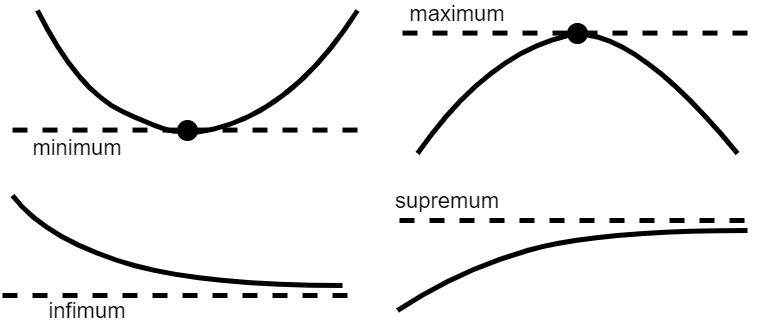
\includegraphics[width=3.2in]{./images/min_max_inf_sup}
  \caption{Minimum, maximum, infimum, and supremum of example functions.}
  \label{figure_min_max_inf_sup}
\end{figure}

\begin{figure}[!t]
  \centering
  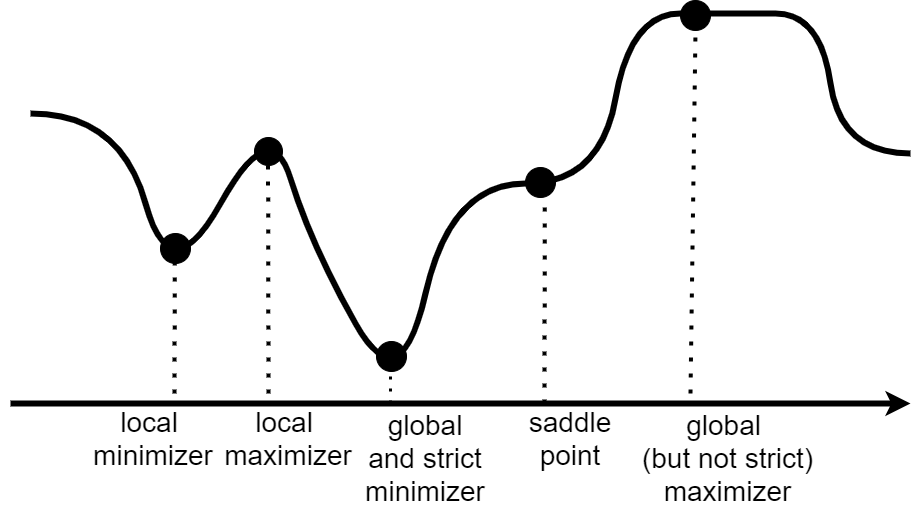
\includegraphics[width=3.2in]{./images/StationaryPoints}
  \caption{Examples for stationary points such as local and global extreme points, strict and non-strict extreme points, and saddle point.}
  \label{figure_StationaryPoints}
\end{figure}

\begin{theorem}[内积]
  Consider two vectors $\boldsymbol{x} = [x_1, \dots, x_d]^\top \in \mathbb{R}^d$ and $\boldsymbol{y} = [y_1, \dots, y_d]^\top \in \mathbb{R}^d$. Their inner product, also called dot product, is:
  \begin{align*}
  & \langle \boldsymbol{x}, \boldsymbol{y} \rangle = \boldsymbol{x}^\top \boldsymbol{y} = \sum_{i=1}^d x_i\, y_i.
  \end{align*}
  We also have inner product between matrices $\boldsymbol{X}, \boldsymbol{Y} \in \mathbb{R}^{d_1 \times d_2}$. Let $\boldsymbol{X}_{ij}$ denote the $(i,j)$-th element of matrix $\boldsymbol{X}$. The inner product of $\boldsymbol{X}$ and $\boldsymbol{Y}$ is:
  \begin{align*}
  & \langle \boldsymbol{X}, \boldsymbol{Y} \rangle = \textbf{tr}(\boldsymbol{X}^\top \boldsymbol{Y}) = \sum_{i=1}^{d_1} \sum_{j=1}^{d_2} \boldsymbol{X}_{i,j}\, \boldsymbol{Y}_{i,j},
  \end{align*}
  where $\textbf{tr}(.)$ denotes the trace of matrix. 
\end{theorem}

\begin{definition}[范数]
  A function $\|\cdot\|: \mathbb{R}^d \rightarrow \mathbb{R}$, $\|\cdot\|: \boldsymbol{x} \mapsto \|\boldsymbol{x}\|$ is a norm if it satisfies:
\begin{enumerate}
  \item $\|\boldsymbol{x}\| \geq 0, \forall \boldsymbol{x}$
  \item $\|a \boldsymbol{x}\| = |a|\, \|\boldsymbol{x}\|, \forall \boldsymbol{x}$ and all scalars $a$
  \item $\|\boldsymbol{x}\| = 0$ if and only if $\boldsymbol{x} = 0$
  \item Triangle inequality: $\|\boldsymbol{x} + \boldsymbol{y}\| \leq \|\boldsymbol{x}\| + \|\boldsymbol{y}\|$.
\end{enumerate}
\end{definition}

\begin{definition}[重要的范数]
  Some important norms for a vector $\boldsymbol{x} = [x_1, \dots, x_d]^\top$ are as follows. 
  The $\ell_p$ norm is:
  \begin{align*}
  & \|\boldsymbol{x}\|_p := \big(|x_1|^p + \dots + |x_d|^p\big)^{1/p},
  \end{align*}
  where $p \geq 1$ and $|.|$ denotes the absolute value. 
  Two well-known $\ell_p$ norms are $\ell_1$ norm and $\ell_2$ norm (also called the Euclidean norm) with $p=1$ and $p=2$, respectively.
  The $\ell_\infty$ norm, also called the infinity norm, the maximum norm, or the Chebyshev norm, is:
  \begin{align*}
  & \|\boldsymbol{x}\|_\infty := \max\{|x_1| + \cdots + |x_d|\}. 
  \end{align*}
  For the matrix $\boldsymbol{X} \in \mathbb{R}^{d_1 \times d_2}$, the $\ell_p$ norm is:
  \begin{align*}
  \|\boldsymbol{X}\|_p := \sup_{\boldsymbol{y} \neq 0} \frac{\|\boldsymbol{X}\boldsymbol{y}\|_p}{\|\boldsymbol{y}\|_p}.
  \end{align*}
  A special case for this is the $\ell_2$ norm, also called the spectral norm or the Euclidean norm. The spectral norm is related to the largest singular value of matrix:
  \begin{align*}
  \|\boldsymbol{X}\|_2 = \sup_{\boldsymbol{y} \neq 0} \frac{\|\boldsymbol{X}\boldsymbol{y}\|_2}{\|\boldsymbol{y}\|_2} = \sqrt{\lambda_{\text{max}}(\boldsymbol{X}^\top \boldsymbol{X})} = \sigma_{\text{max}}(\boldsymbol{X}),
  \end{align*}
  where $\lambda_{\text{max}}(\boldsymbol{X}^\top \boldsymbol{X})$ and $\sigma_{\text{max}}(\boldsymbol{X})$ denote the largest eigenvalue of $\boldsymbol{X}^\top \boldsymbol{X}$ and the largest singular value of $\boldsymbol{X}$, respectively.
  Other specaial cases are the maximum-absolute-column-sum norm ($p=1$) and the maximum-absolute-row-sum norm ($p=\infty$):
  \begin{align*}
  & \|\boldsymbol{X}\|_1 = \sup_{\boldsymbol{y} \neq 0} \frac{\|\boldsymbol{X}\boldsymbol{y}\|_1}{\|\boldsymbol{y}\|_1} = \max_{1 \leq j \leq d_2} \sum_{i=1}^{d_1} |\boldsymbol{X}_{i,j}|, \\
  & \|\boldsymbol{X}\|_\infty = \sup_{\boldsymbol{y} \neq 0} \frac{\|\boldsymbol{X}\boldsymbol{y}\|_\infty}{\|\boldsymbol{y}\|_\infty} = \max_{1 \leq i \leq d_1} \sum_{j=1}^{d_2} |\boldsymbol{X}_{i,j}|.
  \end{align*}
The formulation of the Frobenius norm for a matrix is similar to the formulation of $\ell_2$ norm for a vector:
  \begin{align*}
  \|\boldsymbol{X}\|_F := \sqrt{\sum_{i=1}^{d_1} \sum_{j=1}^{d_2} \boldsymbol{X}_{i,j}^2},
  \end{align*}
where $\boldsymbol{X}_{ij}$ denotes the $(i,j)$-th element of $\boldsymbol{X}$.

The $\ell_{2,1}$ norm of matrix $\boldsymbol{X}$ is:
\begin{align*}
& \|\boldsymbol{X}\|_{2,1} := \sum_{i=1}^{d_1} \sqrt{\sum_{j=1}^{d_2} \boldsymbol{X}_{i,j}^2}.
\end{align*}

The Schatten $\ell_p$ norm of matrix $\boldsymbol{X}$ is:
\begin{align*}
\|\boldsymbol{X}\|_p := \bigg(\sum_{i=1}^{\min(d_1, d_2)} \big(\sigma_i(\boldsymbol{X})\big)^p\bigg)^{1/p},
\end{align*}
where $\sigma_i(\boldsymbol{X})$ denotes the $i$-th singular value of $\boldsymbol{X}$.
A special case of the Schatten norm, with $p=1$, is called the nuclear norm or the trace norm:
\begin{align*}
\|\boldsymbol{X}\|_* := \sum_{i=1}^{\min(d_1, d_2)} \sigma_i(\boldsymbol{X}) = \textbf{tr}\Big(\!\sqrt{\boldsymbol{X}^\top \boldsymbol{X}}\,\Big),
\end{align*}
which is summation of the singular values of matrix. 
Note that similar to use of $\ell_1$ norm of vector for sparsity, the nuclear norm is also used to impose sparsity on matrix. 
\end{definition}

\begin{lemma}
We have:
\begin{align*}
& \|\boldsymbol{x}\|_2^2 = \boldsymbol{x}^\top \boldsymbol{x} = \langle \boldsymbol{x}, \boldsymbol{x} \rangle, \\
& \|\boldsymbol{X}\|_F^2 = \textbf{tr}(\boldsymbol{X}^\top \boldsymbol{X}) = \langle \boldsymbol{X}, \boldsymbol{X} \rangle, 
\end{align*}
which are convex and in quadratic forms. 
\end{lemma}

\begin{figure}[!t]
\centering
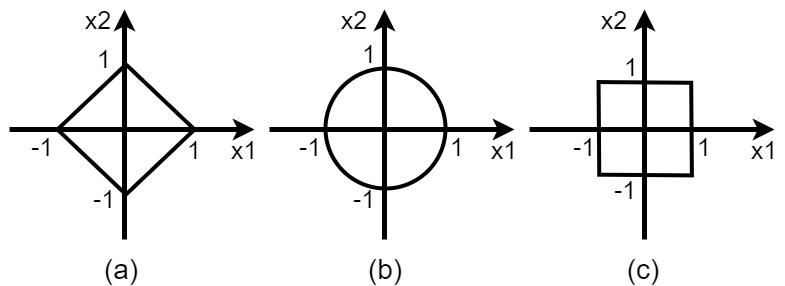
\includegraphics[width=3.2in]{./images/unit_balls}
\caption{The unit balls, in $\mathbb{R}^2$, for (a) $\ell_1$ norm, (b) $\ell_2$ norm, and (c) $\ell_\infty$ norm.}
\label{figure_unit_balls}
\end{figure}

\begin{definition}[Dual norm]
Let $\|.\|$ be a norm on $\mathbb{R}^d$. Its dual norm is:
\begin{align}
\|\boldsymbol{x}\|_* := \sup\{\boldsymbol{x}^\top \boldsymbol{y}\, |\, \|\boldsymbol{y}\| \leq 1\}. 
\end{align}
Note that the notation $\|\cdot\|_*$ should not be confused with the the nuclear norm despite of similarity of notations.
\end{definition}

% % https://en.wikipedia.org/wiki/Norm_(mathematics)#Properties
% https://en.wikipedia.org/wiki/H%C3%B6lder%27s_inequality
\begin{lemma}[H{\"o}lder's \cite{holder1889ueber} and Cauchy-Schwarz inequalities \cite{steele2004cauchy}]
Let $p,q \in [1, \infty]$ and:
\begin{align}\label{Holder_inequality_1p_1q_equals_1}
\frac{1}{p} + \frac{1}{q} = 1.
\end{align}
These $p$ and $q$ are called the H{\"o}lder conjugates of each other. According to the H{\"o}lder's inequality, for functions $f(.)$ and $g(.)$, we have $\|fg\|_1 \leq \|f\|_p \|g\|_q$. 
A corollary of the H{\"o}lder's inequality is that Eq. (\ref{Holder_inequality_1p_1q_equals_1}) holds if the norms $\|.\|_p$ and $\|.\|_q$ are dual of each other. H{\"o}lder's inequality states that:
\begin{align*}
|\boldsymbol{x}^\top \boldsymbol{y}| \leq \|\boldsymbol{x}\|_p \|\boldsymbol{x}\|_q,
\end{align*}
where $p$ and $q$ satisfy Eq. (\ref{Holder_inequality_1p_1q_equals_1}). A special case of the H{\"o}lder's inequality is the Cauchy-Schwarz inequality, stated as $|\boldsymbol{x}^\top \boldsymbol{y}| \leq \|\boldsymbol{x}\|_2 \|\boldsymbol{x}\|_2$.
\end{lemma}

According to Eq. (\ref{Holder_inequality_1p_1q_equals_1}), we have:
\begin{align}\label{equation_dual_norm_calculation}
&\|\cdot\|_p \implies \|\cdot\|_* = \|\cdot\|_{p / (p-1)}, \quad \forall p \in [1, \infty].
\end{align}
For example, the dual norm of $\|.\|_2$ is $\|.\|_2$ again and the dual norm of $\|.\|_1$ is $\|.\|_\infty$. 


\begin{definition}[Cone and dual cone]
A set $\mathcal{K} \subseteq \mathbb{R}^d$ is a cone if:
\begin{enumerate}
\item it contains the origin, i.e., $\boldsymbol{0} \in \mathcal{K}$,
\item $\mathcal{K}$ is a convex set,
\item for each $\boldsymbol{x} \in \mathcal{K}$ and $\lambda \geq 0$, we have $\lambda \boldsymbol{x} \in \mathcal{K}$.
\end{enumerate}
The dual cone of a cone $\mathcal{K}$ is:
\begin{align*}
\mathcal{K}^* := \{\boldsymbol{y}\, |\, \boldsymbol{y}^\top \boldsymbol{x} \geq 0, \forall \boldsymbol{x} \in \mathcal{K}\}.
\end{align*}
An example cone and its dual are depicted in Fig. \ref{figure_dual_cone}-a.
\end{definition}

\begin{figure}[!t]
\centering
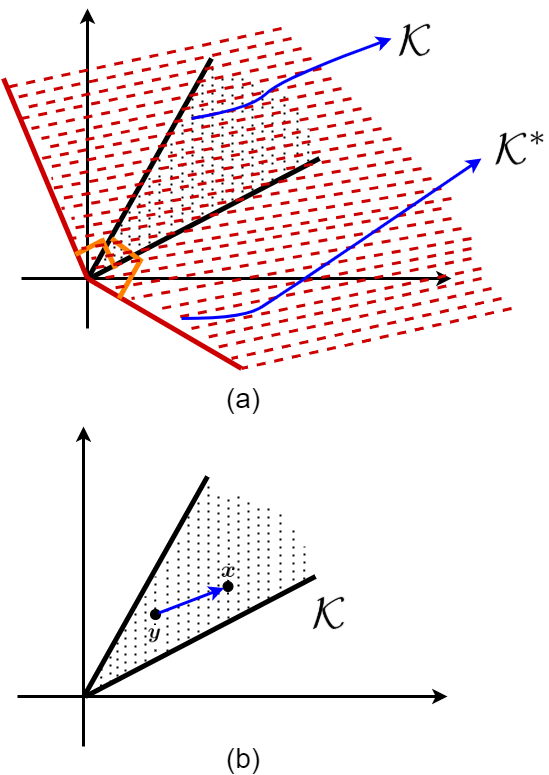
\includegraphics[width=2.8in]{./images/dual_cone}
\caption{(a) A cone $\mathcal{K}$ and its dual cone $\mathcal{K}^*$. Note that the borders of dual cone are perpendicular to the borders of the cone as shown in this figure. (b) An example for the generalized inequality $\boldsymbol{x} \succeq_\mathcal{K} \boldsymbol{y}$. As it is shown, the vector $(\boldsymbol{x} - \boldsymbol{y})$ belongs to the cone $\mathcal{K}$.}
\label{figure_dual_cone}
\end{figure}

\begin{definition}[Proper cone \cite{boyd2004convex}]
A convex cone $\mathcal{K} \subseteq \mathbb{R}^d$ is a proper cone if:
\begin{enumerate}
\item $\mathcal{K}$ is closed, i.e., it contains its boundary, 
\item $\mathcal{K}$ is solid, i.e., its interior is non-empty, 
\item $\mathcal{K}$ is pointed, i.e., it contains no line. In other words, it is not a two-sided cone around the origin.
\end{enumerate}
\end{definition}

\begin{definition}[Generalized inequality \cite{boyd2004convex}]\label{definition_generalized_inequality}
A generalized inequality, defined by a proper cone $\mathcal{K}$, is:
\begin{align*}
\boldsymbol{x} \succeq_\mathcal{K} \boldsymbol{y} \iff \boldsymbol{x} - \boldsymbol{y} \in \mathcal{K}.
\end{align*}
This means $\boldsymbol{x} \succeq_\mathcal{K} \boldsymbol{y} \iff \boldsymbol{x} - \boldsymbol{y} \in \textbf{int}(\mathcal{K})$. 
Note that $\boldsymbol{x} \succeq_\mathcal{K} \boldsymbol{y}$ can also be stated as $\boldsymbol{x} - \boldsymbol{y} \succeq_\mathcal{K} \boldsymbol{0}$.
An example for a generalized inequality is shown in Fig. \ref{figure_dual_cone}-b.
\end{definition}

\begin{definition}[Important examples for generalized inequality]\label{definition_generalized_inequality_examples}
The generalized inequality defined by the non-negative orthant, $\mathcal{K} = \mathbb{R}_+^d$, is the default inequality for vectors $\boldsymbol{x} = [x_1, \dots, x_d]^\top$, $\boldsymbol{y} = [y_1, \dots, y_d]^\top$:
\begin{align*}
\boldsymbol{x} \succeq \boldsymbol{y} \iff \boldsymbol{x} \succeq_{\mathbb{R}_+^d} \boldsymbol{y}.
\end{align*}
It means component-wise inequality:
\begin{align*}
\boldsymbol{x} \succeq \boldsymbol{y} \iff x_i \geq y_i, \quad \forall i \in \{1, \dots, d\}.
\end{align*}
The generalized inequality defined by the positive definite cone, $\mathcal{K} = \mathbb{S}_+^d$, is the default inequality for symmetric matrices $\boldsymbol{X}, \boldsymbol{Y} \in \mathbb{S}^d$:
\begin{align*}
\boldsymbol{X} \succeq \boldsymbol{Y} \iff \boldsymbol{X} \succeq_{\mathbb{S}_+^d} \boldsymbol{Y}.
\end{align*}
It means $(\boldsymbol{X} - \boldsymbol{Y})$ is positive semi-definite. Note that if the inequality is strict, i.e. $\boldsymbol{X} \succ \boldsymbol{Y}$, it means that $(\boldsymbol{X} - \boldsymbol{Y})$ is positive definite.
In conclusion, $\boldsymbol{x} \succeq \boldsymbol{0}$ means all elements of vector $\boldsymbol{x}$ are non-negative and $\boldsymbol{X} \succeq \boldsymbol{0}$ means the matrix $\boldsymbol{X}$ is positive semi-definite. 
\end{definition}

\subsection{Preliminaries on Functions}

% https://en.wikipedia.org/wiki/Fixed_point_(mathematics)
% https://en.wikipedia.org/wiki/Fixed-point_iteration
\begin{definition}[Fixed point]\label{definition_fixed_point}
A fixed point of a function $f(.)$ is a point $\boldsymbol{x}$ which is mapped to itself by the function, i.e., $f(\boldsymbol{x}) = \boldsymbol{x}$.
\end{definition}

\begin{definition}[Convex function]
A function $f(.)$ with domain $\mathcal{D}$ is convex if:
\begin{align}\label{equation_convex_function}
f\big(\alpha \boldsymbol{x} + (1-\alpha) \boldsymbol{y}\big) \leq \alpha f(\boldsymbol{x}) + (1-\alpha) f(\boldsymbol{y}),
\end{align}
$\forall \boldsymbol{x}, \boldsymbol{y} \in \mathcal{D}$, where $\alpha \in [0,1]$. Eq. (\ref{equation_convex_function}) is depicted in Fig. \ref{figure_convex_function}-a.

Moreover, if the function $f(.)$ is differentiable, it is convex if:
\begin{align}\label{equation_convex_function_firstDerivative}
f(\boldsymbol{x}) \geq f(\boldsymbol{y}) + \nabla f(\boldsymbol{y})^\top (\boldsymbol{x} - \boldsymbol{y}),
\end{align}
$\forall \boldsymbol{x}, \boldsymbol{y} \in \mathcal{D}$. 
Eq. (\ref{equation_convex_function_firstDerivative}) is depicted in Fig. \ref{figure_convex_function}-b.

Moreover, if the function $f(.)$ is twice differentiable, it is convex if its second-order derivative is positive semi-definite:
\begin{align}\label{equation_convex_function_secondDerivative}
\nabla^2 f(\boldsymbol{x}) \succeq \boldsymbol{0},
\end{align}
$\forall \boldsymbol{x} \in \mathcal{D}$. 
\end{definition}
Each of the Eqs. (\ref{equation_convex_function}), (\ref{equation_convex_function_firstDerivative}), and (\ref{equation_convex_function_secondDerivative}) is a definition for the convex function. 
Note that if $\geq$ is changed to $\leq$ in Eqs. (\ref{equation_convex_function}) and (\ref{equation_convex_function_firstDerivative}) or if $\succeq$ is changed to $\preceq$ in Eq. (\ref{equation_convex_function_secondDerivative}), the function is \textit{concave}. 

\begin{figure}[!t]
\centering
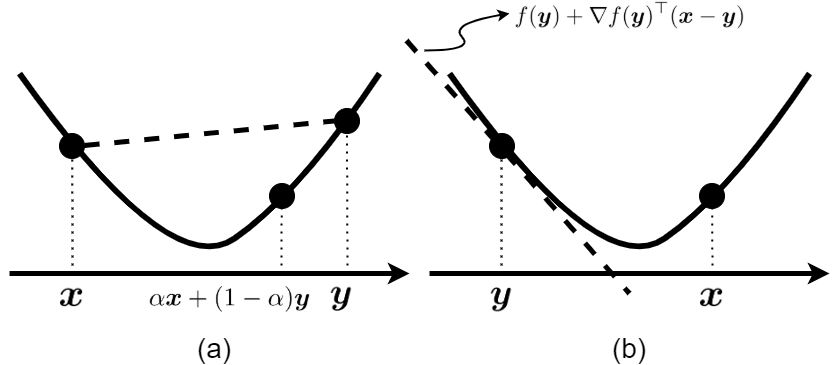
\includegraphics[width=3.2in]{./images/convex_function}
\caption{Two definitions for the convex function: (a) Eq. (\ref{equation_convex_function}) meaning that the function value for the point $\alpha \boldsymbol{x} + (1-\alpha) \boldsymbol{y}$ is less than or equal to the hyper-line $\alpha f(\boldsymbol{x}) + (1-\alpha) f(\boldsymbol{y})$, and (b) Eq. (\ref{equation_convex_function_firstDerivative}) meaning that the function value for $\boldsymbol{x}$, i.e. $f(\boldsymbol{x})$, falls above the hyper-line $f(\boldsymbol{y}) + \nabla f(\boldsymbol{y})^\top (\boldsymbol{x} - \boldsymbol{y}), \forall \boldsymbol{x}, \boldsymbol{y} \in \mathcal{D}$.}
\label{figure_convex_function}
\end{figure}

\begin{definition}[Strongly convex function]
A differential function $f(.)$ with domain $\mathcal{D}$ is $\mu$-strongly convex if:
\begin{align}\label{equation_strongly_convex_function_firstDerivative}
f(\boldsymbol{x}) \geq f(\boldsymbol{y}) + \nabla f(\boldsymbol{y})^\top (\boldsymbol{x} - \boldsymbol{y}) + \frac{\mu}{2} \|\boldsymbol{x} - \boldsymbol{y}\|_2^2,
\end{align}
$\forall \boldsymbol{x}, \boldsymbol{y} \in \mathcal{D}$ and $\mu > 0$.

Moreover, if the function $f(.)$ is twice differentiable, it is $\mu$-strongly convex if its second-order derivative is positive semi-definite:
\begin{align}\label{equation_strongly_convex_function_secondDerivative}
\boldsymbol{y}^\top \nabla^2 f(\boldsymbol{x}) \boldsymbol{y} \geq \mu \|\boldsymbol{y}\|_2^2,
\end{align}
$\forall \boldsymbol{x}, \boldsymbol{y} \in \mathcal{D}$ and $\mu > 0$.
A strongly convex function has a unique minimizer. See Fig. \ref{figure_stronglyConvex} for difference of convex and strongly convex functions. 
\end{definition}

\begin{figure}[!t]
\centering
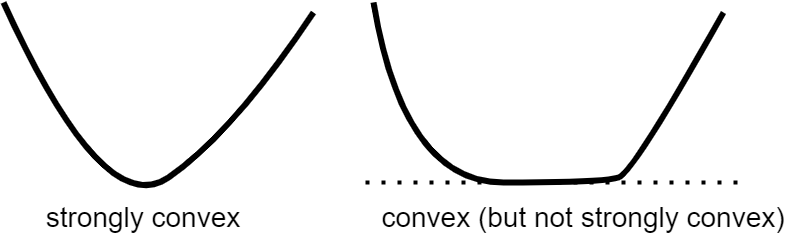
\includegraphics[width=3.2in]{./images/stronglyConvex}
\caption{Comparison of strongly convex and convex functions. The strongly convex function has only one strict minimizer while the convex function can have multiple minimizers with equal function values.}
\label{figure_stronglyConvex}
\end{figure}


% \begin{definition}[H{\"o}lder smoothness \cite{tsybakov2009introduction}]
% For a vector $\boldsymbol{s} = [s_1, \dots, s_d]^\top$, let $|\boldsymbol{s}| := s_1 + \dots + s_d$ and $D^s := \frac{\partial^{|\boldsymbol{s}|}}{\partial \boldsymbol{x}_1^{s_1} \dots \partial \boldsymbol{x}_1^{s_d}}$.
% A function $f(.)$ belongs to a H{\"o}lder space $H(\beta, L)$, with smoothness parameter $\beta$ and the radius $L$ for ball (as the space can be seen as a ball), if:
% \begin{align}
% \big\|D^s f(\boldsymbol{x}) - D^s f(\boldsymbol{y})\big\|_2 \leq L\, \|\boldsymbol{x} - \boldsymbol{y}\|_2^{\beta-1}.
% \end{align}
% The H{\"o}lder space relates to local smoothness. This smoothness is called the H{\"o}lder smoothness. 
% \end{definition}

\begin{definition}[H{\"o}lder and Lipschitz smoothness]
A function $f(.)$ with domain $\mathcal{D}$ belongs to a H{\"o}lder space $H(\alpha, L)$, with smoothness parameter $\alpha$ and the radius $L$ for ball (as the space can be seen as a ball), if:
\begin{align}
|f(\boldsymbol{x}) - f(\boldsymbol{y})| \leq L\, \|\boldsymbol{x} - \boldsymbol{y}\|_2^{\alpha}, \quad \forall \boldsymbol{x}, \boldsymbol{y} \in \mathcal{D}.
\end{align}
The H{\"o}lder space relates to local smoothness. A function in this space is called H{\"o}lder smooth (or H{\"o}lder continuous). 
A function is Lipschitz smooth (or Lipschitz continuous) if it is H{\"o}lder smooth with $\alpha=1$:
\begin{align}
|f(\boldsymbol{x}) - f(\boldsymbol{y})| \leq L\, \|\boldsymbol{x} - \boldsymbol{y}\|_2, \quad \forall \boldsymbol{x}, \boldsymbol{y} \in \mathcal{D}.
\end{align}
The parameter $L$ is called the Lipschitz constant.
A function with Lipschitz smoothness (with Lipschitz constant $L$) is called $L$-smooth. 
\end{definition}
H{\"o}lder and Lipschitz smoothness are used in many convergence and correctness proofs for optimization (e.g., see \cite{liu2021smooth}). 

The following lemma, which is based on the fundamental theorem of calculus, is widely used in proofs of optimization methods. 
\begin{lemma}[Fundamental theorem of calculus for multivariate functions]
Consider a differentiable function $f(.)$ with domain $\mathcal{D}$.
For any $\boldsymbol{x}, \boldsymbol{y} \in \mathcal{D}$, we have:
\begin{equation}\label{equation_fundamental_theorem_calculus}
\begin{aligned}
&f(\boldsymbol{y}) = f(\boldsymbol{x}) + \nabla f(\boldsymbol{x})^\top (\boldsymbol{y} - \boldsymbol{x}) \\
&~~~~~~+ \int_0^1 \Big(\nabla f\big(\boldsymbol{x} + t(\boldsymbol{y} - \boldsymbol{x})\big) - \nabla f(\boldsymbol{x}) \Big)^\top (\boldsymbol{y} - \boldsymbol{x}) dt \\
&~~~~~= f(\boldsymbol{x}) + \nabla f(\boldsymbol{x})^\top (\boldsymbol{y} - \boldsymbol{x}) + o(\boldsymbol{y} - \boldsymbol{x}),
\end{aligned}
\end{equation}
where $o(.)$ is the small-$o$ complexity.
\end{lemma}

\begin{lemma}[Corollary of the fundamental theorem of calculus]\label{lemma_fundamental_theorem_calculus_corollary}
Consider a differentiable function $f(.)$, with domain $\mathcal{D}$, whose gradient is $L$-smooth:
\begin{align}\label{equation_gradient_L_smooth}
|\nabla f(\boldsymbol{x}) - \nabla f(\boldsymbol{y})| \leq L\, \|\boldsymbol{x} - \boldsymbol{y}\|_2, \quad \forall \boldsymbol{x}, \boldsymbol{y} \in \mathcal{D}.
\end{align}
For any $\boldsymbol{x}, \boldsymbol{y} \in \mathcal{D}$, we have:
\begin{equation}\label{equation_fundamental_theorem_calculus_Lipschitz}
\begin{aligned}
&f(\boldsymbol{y}) \leq f(\boldsymbol{x}) + \nabla f(\boldsymbol{x})^\top (\boldsymbol{y} - \boldsymbol{x}) + \frac{L}{2} \|\boldsymbol{y} - \boldsymbol{x}\|_2^2.
\end{aligned}
\end{equation}
\end{lemma}
\begin{proof}
\begin{align*}
&f(\boldsymbol{y}) \overset{(\ref{equation_fundamental_theorem_calculus})}{=} f(\boldsymbol{x}) + \nabla f(\boldsymbol{x})^\top (\boldsymbol{y} - \boldsymbol{x}) \\
&~~~~~~+ \int_0^1 \Big(\nabla f\big(\boldsymbol{x} + t(\boldsymbol{y} - \boldsymbol{x})\big) - \nabla f(\boldsymbol{x}) \Big)^\top (\boldsymbol{y} - \boldsymbol{x}) dt \\
&\overset{(a)}{\leq} f(\boldsymbol{x}) + \nabla f(\boldsymbol{x})^\top (\boldsymbol{y} - \boldsymbol{x}) \\
&~~~+ \int_0^1 \|\nabla f\big(\boldsymbol{x} + t(\boldsymbol{y} - \boldsymbol{x})\big) - \nabla f(\boldsymbol{x}) \|_2 \|\boldsymbol{y} - \boldsymbol{x}\|_2 dt \\
&\overset{(b)}{\leq} f(\boldsymbol{x}) + \nabla f(\boldsymbol{x})^\top (\boldsymbol{y} - \boldsymbol{x}) + \int_0^1 L t \|\boldsymbol{y} - \boldsymbol{x}\|_2^2 dt \\
&= f(\boldsymbol{x}) + \nabla f(\boldsymbol{x})^\top (\boldsymbol{y} - \boldsymbol{x}) + L \|\boldsymbol{y} - \boldsymbol{x}\|_2^2 \int_0^1 t dt \\
&= f(\boldsymbol{x}) + \nabla f(\boldsymbol{x})^\top (\boldsymbol{y} - \boldsymbol{x}) + \frac{L}{2} \|\boldsymbol{y} - \boldsymbol{x}\|_2^2,
\end{align*}
where $(a)$ is because of the Cauchy-Schwarz inequality and $(b)$ is because, according to Eq. (\ref{equation_gradient_L_smooth}), we have $\|\nabla f(\boldsymbol{x} + t(\boldsymbol{y} - \boldsymbol{x})) - \nabla f(\boldsymbol{x}) \|_2 = L \|\boldsymbol{x} + t(\boldsymbol{y} - \boldsymbol{x}) - \boldsymbol{x}\|_2 = L t \|\boldsymbol{y} - \boldsymbol{x}\|_2$. Q.E.D.
\end{proof}

The following lemma is useful for proofs of convergence of first-order methods. 
\begin{lemma}\label{lemma_function_and_gradient_difference_bounds}
Consider a convex and differentiable function $f(.)$, with domain $\mathcal{D}$, whose gradient is $L$-smooth (see Eq. (\ref{equation_gradient_L_smooth})). We have:
\begin{align}
f(\boldsymbol{y}) - f(\boldsymbol{x}) \leq &\,\nabla f(\boldsymbol{y})^\top (\boldsymbol{y} - \boldsymbol{x}) \nonumber \\
&- \frac{1}{2 L} \|\nabla f(\boldsymbol{y}) - \nabla f(\boldsymbol{x})\|_2^2, \label{equation_lemma_fy_fx_grady_y_x}
\end{align}
\begin{align}
& \big( \nabla f(\boldsymbol{y}) - \nabla f(\boldsymbol{x}) \big)^\top (\boldsymbol{y} - \boldsymbol{x}) \geq \frac{1}{L} \|\nabla f(\boldsymbol{y}) - \nabla f(\boldsymbol{x})\|_2^2. \label{equation_lemma_gradfy_gradfx_y_x}
\end{align}
\end{lemma}
\begin{proof}
\textbf{-- Proof for the first equation:}
As $f(.)$ is convex, according to Eq. (\ref{equation_convex_function_firstDerivative}), 
\begin{align}
&f(\boldsymbol{z}) - f(\boldsymbol{y}) \geq \nabla f(\boldsymbol{y})^\top (\boldsymbol{z} - \boldsymbol{y}) \nonumber \\
&\implies f(\boldsymbol{y}) - f(\boldsymbol{z}) \leq \nabla f(\boldsymbol{y})^\top (\boldsymbol{y} - \boldsymbol{z}). \label{equation_fz_fy_gradf_z_y}
\end{align}
\begin{align}\label{equation_fy_fz_fz_fx}
&f(\boldsymbol{y}) - f(\boldsymbol{x}) = \big(f(\boldsymbol{y}) - f(\boldsymbol{z})\big) + \big(f(\boldsymbol{z}) - f(\boldsymbol{x})\big).
\end{align}
Also, according to Eq. (\ref{equation_fundamental_theorem_calculus_Lipschitz}), we have:
\begin{align}\label{equation_fz_fx_gradf_z_x_L_z_x}
&f(\boldsymbol{z}) - f(\boldsymbol{x}) \leq \nabla f(\boldsymbol{x})^\top (\boldsymbol{z} - \boldsymbol{x}) + \frac{L}{2} \|\boldsymbol{z} - \boldsymbol{x}\|_2^2.
\end{align}
Using Eqs. (\ref{equation_fz_fy_gradf_z_y}) and (\ref{equation_fz_fx_gradf_z_x_L_z_x}) in Eq. (\ref{equation_fy_fz_fz_fx}) gives:
\begin{align*}
f(\boldsymbol{y}) - f(\boldsymbol{x}) \leq &\,\nabla f(\boldsymbol{y})^\top (\boldsymbol{y} - \boldsymbol{z}) + \nabla f(\boldsymbol{x})^\top (\boldsymbol{z} - \boldsymbol{x}) \\
&+ \frac{L}{2} \|\boldsymbol{z} - \boldsymbol{x}\|_2^2.
\end{align*}
For this, we can minimize this upper-bound (the right-hand side) by setting its derivative w.r.t. $\boldsymbol{z}$ to zero. It gives:
\begin{align*}
\boldsymbol{z} = \boldsymbol{x} - \frac{1}{L} \big(\nabla f(\boldsymbol{x}) - \nabla f(\boldsymbol{y})\big).
\end{align*}
Putting this in the upper-bound gives:
\begin{align*}
&f(\boldsymbol{y}) - f(\boldsymbol{x}) \leq \nabla f(\boldsymbol{y})^\top (\boldsymbol{y} - \boldsymbol{x}) \\
&+ \frac{1}{L} \nabla f(\boldsymbol{y})^\top (\nabla f(\boldsymbol{x}) - \nabla f(\boldsymbol{y})) \\
&- \frac{1}{L} \nabla f(\boldsymbol{x})^\top (\nabla f(\boldsymbol{x}) - \nabla f(\boldsymbol{y})) \\
&+ \frac{L}{2} \frac{1}{L^2} \|\nabla f(\boldsymbol{x}) - \nabla f(\boldsymbol{y})\|_2^2 \\
&\overset{(a)}{=} \nabla f(\boldsymbol{y})^\top (\boldsymbol{y} - \boldsymbol{x}) - \frac{1}{L} \|\nabla f(\boldsymbol{x}) - \nabla f(\boldsymbol{y})\|_2^2 \\
&+ \frac{1}{2L} \|\nabla f(\boldsymbol{x}) - \nabla f(\boldsymbol{y})\|_2^2 \\
&= \nabla f(\boldsymbol{y})^\top (\boldsymbol{y} - \boldsymbol{x}) - \frac{1}{2L} \|\nabla f(\boldsymbol{x}) - \nabla f(\boldsymbol{y})\|_2^2,
\end{align*}
were $(a)$ is because $\|\nabla f(\boldsymbol{x}) - \nabla f(\boldsymbol{y})\|_2^2 = (\nabla f(\boldsymbol{x}) - \nabla f(\boldsymbol{y}))^\top (\nabla f(\boldsymbol{x}) - \nabla f(\boldsymbol{y}))$. 

\textbf{-- Proof for the second equation:}
If we exchange the points $\boldsymbol{x}$ and $\boldsymbol{y}$ in Eq. (\ref{equation_lemma_fy_fx_grady_y_x}), we have:
\begin{align}
f(\boldsymbol{x}) - f(\boldsymbol{y}) \leq &\,\nabla f(\boldsymbol{x})^\top (\boldsymbol{x} - \boldsymbol{y}) \nonumber \\
&- \frac{1}{2 L} \|\nabla f(\boldsymbol{y}) - \nabla f(\boldsymbol{x})\|_2^2. \label{equation_lemma_fy_fx_grady_y_x_2}
\end{align}
Adding Eqs. (\ref{equation_lemma_fy_fx_grady_y_x}) and (\ref{equation_lemma_fy_fx_grady_y_x_2}) gives:
\begin{align*}
0 \leq &\,(\nabla f(\boldsymbol{y}) - \nabla f(\boldsymbol{x}))^\top (\boldsymbol{y} - \boldsymbol{x}) - \frac{1}{L} \|\nabla f(\boldsymbol{y}) - \nabla f(\boldsymbol{x})\|_2^2.
\end{align*}
Q.E.D.
\end{proof}

\subsection{Preliminaries on Optimization}

\begin{definition}[Local and global minimizers]
A point $\boldsymbol{x} \in \mathcal{D}$ is a local minimizer of function $f(.)$ if and only if:
\begin{align}\label{equation_local_minimizer}
\exists\, \epsilon > 0 : \forall \boldsymbol{y} \in \mathcal{D},\, \|\boldsymbol{y} - \boldsymbol{x}\|_2 \leq \epsilon \implies f(\boldsymbol{x}) \leq f(\boldsymbol{y}),
\end{align}
meaning that in an $\epsilon$-neighborhood of $\boldsymbol{x}$, the value of function is minimum at $\boldsymbol{x}$.
A point $\boldsymbol{x} \in \mathcal{D}$ is a global minimizer of function $f(.)$ if and only if:
\begin{align}\label{equation_global_minimizer}
f(\boldsymbol{x}) \leq f(\boldsymbol{y}), \quad \forall \boldsymbol{y} \in \mathcal{D}.
\end{align}
See Fig. \ref{figure_StationaryPoints} for examples of local minimizer and maximizer.
\end{definition}

\begin{definition}[Strict minimizers]
In Eqs. (\ref{equation_local_minimizer}) and (\ref{equation_global_minimizer}), if we have $f(\boldsymbol{x}) < f(\boldsymbol{y})$ rather than $f(\boldsymbol{x}) \leq f(\boldsymbol{y})$, the minimizer is a strict local and global minimizer, respectively. 
See Fig. \ref{figure_StationaryPoints} for examples of strict/non-strict minimizer and maximizer.
\end{definition}

\begin{lemma}[Minimizer in convex function]\label{lemma_global_min_convex_function}
In a convex function, any local minimizer is a global minimizer. 
\end{lemma}
\begin{proof}
Consider any $\boldsymbol{y} \in \mathcal{D}$. We define $\boldsymbol{z} := \alpha \boldsymbol{y} + (1 - \alpha) \boldsymbol{x}$. We choose a small enough $\alpha$ to have $\|\boldsymbol{z} - \boldsymbol{x}\|_2 \leq \epsilon$. Hence:
\begin{align*}
\epsilon &\geq \|\boldsymbol{z} - \boldsymbol{x}\|_2 = \|\alpha \boldsymbol{y} + (1 - \alpha) \boldsymbol{x}-\boldsymbol{x}\|_2 = \|\alpha \boldsymbol{y} - \alpha \boldsymbol{x}\|_2 \\
&= \alpha \|\boldsymbol{y} - \boldsymbol{x}\|_2 \implies \alpha \leq \frac{\epsilon}{\|\boldsymbol{y} - \boldsymbol{x}\|_2}.
\end{align*}
As $\alpha \in [0,1]$, we should have $0 \leq \alpha \min(\epsilon / \|\boldsymbol{y} - \boldsymbol{x}\|_2, 1)$.
As $\boldsymbol{x}$ is a local minimizer, according to Eq. (\ref{equation_local_minimizer}), we have $\exists\, \epsilon > 0 : \forall \boldsymbol{z} \in \mathcal{D},\, \|\boldsymbol{z} - \boldsymbol{x}\|_2 \leq \epsilon \implies f(\boldsymbol{x}) \leq f(\boldsymbol{z})$.
As the function is convex, according to Eq. (\ref{equation_convex_function}), we have $f(\boldsymbol{z}) = f\big(\alpha \boldsymbol{y} + (1-\alpha) \boldsymbol{x}\big) \leq \alpha f(\boldsymbol{y}) + (1-\alpha) f(\boldsymbol{x})$ (n.b. we have exchanged the variables $\boldsymbol{x}$ and $\boldsymbol{y}$ in Eq. (\ref{equation_convex_function})).
Hence, overall, we have:
\begin{align*}
&f(\boldsymbol{x}) \leq f(\boldsymbol{z}) \leq \alpha f(\boldsymbol{y}) + (1-\alpha) f(\boldsymbol{x}) \\
&\implies f(\boldsymbol{x}) - (1-\alpha) f(\boldsymbol{x}) \leq \alpha f(\boldsymbol{y}) \\
&\implies \alpha f(\boldsymbol{x}) \leq \alpha f(\boldsymbol{y}) \implies f(\boldsymbol{x}) \leq f(\boldsymbol{y}), \forall \boldsymbol{y} \in \mathcal{D}.
\end{align*}
So, $\boldsymbol{x}$ is the global minimizer. Q.E.D.
\end{proof}

\begin{corollary}\label{corollary_only_one_min_convex_function}
In a convex function, there exists only one local minimizer which is the global minimizer. As an imagination, a convex function is like a multi-dimensional bowl with only one minimizer. 
\end{corollary}

\begin{lemma}[Gradient of a convex function at the minimizer point]\label{lemma_minimizer_gradient_zero}
When the function $f(.)$ is convex and differentiable, a point $\boldsymbol{x}^*$ is a minimizer if and only if $\nabla f(\boldsymbol{x}^*) = \boldsymbol{0}$.
\end{lemma}
\begin{proof}
\textbf{-- Proof for side} ($\boldsymbol{x}^*$ is minimizer $\implies$ $\nabla f(\boldsymbol{x}^*) = \boldsymbol{0}$):

According to the definition of directional derivative, we have:
\begin{align*}
\nabla f(\boldsymbol{x})^\top (\boldsymbol{y} - \boldsymbol{x}) = \lim_{t \rightarrow 0} \frac{f(\boldsymbol{x} + t(\boldsymbol{y} - \boldsymbol{x})) - f(\boldsymbol{x})}{t}.
\end{align*}
For a minimizer $\boldsymbol{x}^*$, we have $f(\boldsymbol{x}^*) \leq f(\boldsymbol{x}^* + t(\boldsymbol{y} - \boldsymbol{x}^*))$ because it minimizes $f(.)$ for a neighborhood around it (n.b. $\boldsymbol{x}^* + t(\boldsymbol{y} - \boldsymbol{x}^*)$ is a neighborhood of $\boldsymbol{x}^*$ because $t$ tends to zero). Hence, we have:
\begin{align*}
0 &\leq \lim_{t \rightarrow 0} \frac{f(\boldsymbol{x}^* + t(\boldsymbol{y} - \boldsymbol{x}^*)) - f(\boldsymbol{x}^*)}{t} \\
&= \nabla f(\boldsymbol{x}^*)^\top (\boldsymbol{y} - \boldsymbol{x}^*).
\end{align*}
As $\boldsymbol{y}$ can be any point in the domain $\mathcal{D}$, we can choose it to be $\boldsymbol{y} = \boldsymbol{x}^* - \nabla f(\boldsymbol{x}^*)$ so we have $\nabla f(\boldsymbol{x}^*) = \boldsymbol{x}^* - \boldsymbol{y}$ and therefore:
\begin{align*}
0 &\leq \nabla f(\boldsymbol{x}^*)^\top (\boldsymbol{y} - \boldsymbol{x}^*) = - \nabla f(\boldsymbol{x}^*)^\top \nabla f(\boldsymbol{x}^*) \\
&= - \|\nabla f(\boldsymbol{x}^*)\|_2^2 \leq 0 \implies \nabla f(\boldsymbol{x}^*) = \boldsymbol{0}. 
\end{align*}

\textbf{-- Proof for side} ($\nabla f(\boldsymbol{x}^*) = \boldsymbol{0}$ $\implies$ $\boldsymbol{x}^*$ is minimizer):

As the function $f(.)$ is convex, according to Eq. (\ref{equation_convex_function_firstDerivative}), we have:
\begin{align*}
f(\boldsymbol{y}) \geq f(\boldsymbol{x}^*) + \nabla f(\boldsymbol{x}^*)^\top (\boldsymbol{y} - \boldsymbol{x}^*),
\end{align*}
$\forall \boldsymbol{y} \in \mathcal{D}$. As we have $\nabla f(\boldsymbol{x}^*) = \boldsymbol{0}$, we can say $f(\boldsymbol{y}) \geq f(\boldsymbol{x}^*), \forall \boldsymbol{y}$. So, $\boldsymbol{x}^*$ is the global minimizer.
\end{proof}

\begin{definition}[Stationary, extremum, and saddle points]
In a general (not-necessarily-convex) function $f(.)$, a point $\boldsymbol{x}^*$ is a stationary if and only if $\nabla f(\boldsymbol{x}^*) = \boldsymbol{0}$. 
By passing through a saddle point, the sign of the second derivative flips to the opposite sign.  
Minimizer and maximizer points (locally or globally) minimize and maximize the function, respectively. A saddle point is neither minimizer nor maximizer, although the gradient at a saddle point is zero. 
Both minimizer and maximizer are also called the extremum points. 
As Fig. \ref{figure_StationaryPoints} shows, some of  stationary point can be either a minimizer, a maximizer, or a saddle point of function.
\end{definition}

\begin{lemma}[First-order optimality condition]\label{lemma_first_order_optimality_condition}
If $\boldsymbol{x}^*$ is a local minimizer for a differentiable function $f(.)$, then:
\begin{align}\label{equation_first_order_optimality_condition}
\nabla f(\boldsymbol{x}^*) = \boldsymbol{0}.
\end{align}
Note that if $f(.)$ is convex, this equation is a necessary and sufficient condition for a minimizer. 
\end{lemma}
\begin{proof}
As $\boldsymbol{x}^*$ is a local minimizer, according to Eq. (\ref{equation_local_minimizer}), we have $\exists\, \epsilon > 0 : \forall \boldsymbol{y} \in \mathcal{D},\, \|\boldsymbol{y} - \boldsymbol{x}^*\|_2 \leq \epsilon \implies f(\boldsymbol{x}^*) \leq f(\boldsymbol{y})$.
Also, by Eq. (\ref{equation_fundamental_theorem_calculus}), we have $f(\boldsymbol{y}) = f(\boldsymbol{x}^*) + \nabla f(\boldsymbol{x}^*)^\top (\boldsymbol{y} - \boldsymbol{x}^*) + o(\boldsymbol{y} - \boldsymbol{x}^*)$. From these two, we have:
\begin{align*}
&f(\boldsymbol{x}^*) \leq f(\boldsymbol{x}^*) + \nabla f(\boldsymbol{x}^*)^\top (\boldsymbol{y} - \boldsymbol{x}^*) + o(\boldsymbol{y} - \boldsymbol{x}^*) \\
&\implies \nabla f(\boldsymbol{x}^*)^\top (\boldsymbol{y} - \boldsymbol{x}^*) \geq 0.
\end{align*}
As $\boldsymbol{y}$ can be any point in the domain $\mathcal{D}$, we can choose it to be $\boldsymbol{y} = \boldsymbol{x}^* - \nabla f(\boldsymbol{x}^*)$ so we have $\nabla f(\boldsymbol{x}^*) = \boldsymbol{x}^* - \boldsymbol{y}$ and therefore $\nabla f(\boldsymbol{x}^*)^\top (\boldsymbol{y} - \boldsymbol{x}^*) = -\|\nabla f(\boldsymbol{x}^*)\|_2^2 \geq 0$. Hence, $\nabla f(\boldsymbol{x}^*) = 0$. Q.E.D.
\end{proof}
Note that if setting the derivative to zero, i.e. Eq. (\ref{equation_first_order_optimality_condition}), gives a closed-form solution for $\boldsymbol{x}^*$, the optimization is done. Otherwise, one should start with some random initialized solution and iteratively update it using the gradient. First-order or second-order methods can be used for iterative optimization (see Sections \ref{section_first_order_methods} and \ref{section_second_order_methods}). 

\begin{definition}[Arguments of minimization and maximization]
In the domain of function, the point which minimizes (resp. maximizes) the function $f(.)$ is the argument for the minimization (resp. maximization) of function. The minimizer and maximizer of function are denoted by $\arg\min_{\boldsymbol{x}} f(\boldsymbol{x})$ and $\arg\max_{\boldsymbol{x}} f(\boldsymbol{x})$, respectively. 
\end{definition}

\begin{remark}
We can convert convert maximization to minimization and vice versa: 
\begin{equation}\label{equation_max_min_conversion}
\begin{aligned}
& \underset{\boldsymbol{x}}{\text{maximize}}\,\,\, f(\boldsymbol{x}) = -\,\underset{\boldsymbol{x}}{\text{minimize}}\,\,\, \big(\!\!-\!f(\boldsymbol{x})\big), \\
& \underset{\boldsymbol{x}}{\text{minimize}}\,\,\, f(\boldsymbol{x}) = -\,\underset{\boldsymbol{x}}{\text{maximize}}\,\,\, \big(\!\!-\!f(\boldsymbol{x})\big).
\end{aligned}
\end{equation}
We can have similar conversions for the arguments of maximization and minimization but we the sign of optimal value of function is not important in argument, we do not have the negative sign before maximization and minimization:
\begin{equation}
\begin{aligned}
& \arg\max_{\boldsymbol{x}} f(\boldsymbol{x}) = \arg\min_{\boldsymbol{x}} \big(\!\!-\!f(\boldsymbol{x})\big), \\
& \arg\min_{\boldsymbol{x}} f(\boldsymbol{x}) = \arg\max_{\boldsymbol{x}} \big(\!\!-\!f(\boldsymbol{x})\big).
\end{aligned}
\end{equation}
\end{remark}

% https://www2.cs.uic.edu/~zhangx/teaching/agm.pdf
\begin{definition}[Convergence rates]\label{definition_convergence_rate}
If any sequence $\{\epsilon_0, \epsilon_1, \dots, \epsilon_{k}, \epsilon_{k+1}, \dots\}$ converges, its convergence rate has one of the following cases:
\begin{align}
\lim_{k \rightarrow \infty} \frac{\epsilon_{k+1}}{\epsilon_k} = 
\left\{
    \begin{array}{ll}
        0 & \mbox{superlinear rate}, \\
        \in (0,1) & \mbox{linear rate}, \\
        1 & \mbox{sublinear rate}.
    \end{array}
\right.
\end{align}
\end{definition}

\subsection{Preliminaries on Derivative}

\begin{remark}[Dimensionality of derivative]\label{remark_dimensionality_of_derivative}
Consider a function $f: \mathbb{R}^{d_1} \rightarrow \mathbb{R}^{d_2}$, $f: \boldsymbol{x} \mapsto f(\boldsymbol{x})$.
Derivative of function $f(\boldsymbol{x}) \in \mathbb{R}^{d_2}$ with respect to (w.r.t.) $\boldsymbol{x} \in \mathbb{R}^{d_1}$ has dimensionality $(d_1 \times d_2)$. This is because tweaking every element of $\boldsymbol{x} \in \mathbb{R}^{d_1}$ can change every element of $f(\boldsymbol{x}) \in \mathbb{R}^{d_2}$. The $(i,j)$-th element of the $(d_1 \times d_2)$-dimensional derivative states the amount of change in the $j$-th element of $f(\boldsymbol{x})$ resulted by changing the $i$-th element of $\boldsymbol{x}$. 

Note that one can use a transpose of the derivative as the derivative. This is okay as long as the dimensionality of other terms in equations of optimization coincide (i.e., they are all transposed). In that case, the dimensionality of derivative is $(d_2 \times d_1)$ where the $(i,j)$-th element of derivative states the amount of change in the $i$-th element of $f(\boldsymbol{x})$ resulted by changing the $j$-th element of $\boldsymbol{x}$. 

Some examples of derivatives are as follows. 
\begin{itemize}\setlength\itemsep{0.01em}
\item If the function is $f: \mathbb{R} \rightarrow \mathbb{R}, f: x \mapsto f(x)$, the derivative $(\partial f(x) / \partial x) \in \mathbb{R}$ is a scalar because changing the scalar $\boldsymbol{x}$ can change the scalar $f(\boldsymbol{x})$.
\item If the function is $f: \mathbb{R}^{d} \rightarrow \mathbb{R}, f: \boldsymbol{x} \mapsto f(\boldsymbol{x})$, the derivative $(\partial f(\boldsymbol{x}) / \partial \boldsymbol{x}) \in \mathbb{R}^d$ is a vector because changing every element of the vector $\boldsymbol{x}$ can change the scalar $f(\boldsymbol{x})$.
\item If the function is $f: \mathbb{R}^{d_1 \times d_2} \rightarrow \mathbb{R}, f: \boldsymbol{X} \mapsto f(\boldsymbol{X})$, the derivative $(\partial f(\boldsymbol{X}) / \partial \boldsymbol{X}) \in \mathbb{R}^{d_1 \times d_2}$ is a matrix because changing every element of the matrix $\boldsymbol{X}$ can change the scalar $f(\boldsymbol{X})$.
\item If the function is $f: \mathbb{R}^{d_1} \rightarrow \mathbb{R}^{d_2}, f: \boldsymbol{x} \mapsto f(\boldsymbol{x})$, the derivative $(\partial f(\boldsymbol{x}) / \partial \boldsymbol{x}) \in \mathbb{R}^{d_1 \times d_2}$ is a matrix because changing every element of the vector $\boldsymbol{x}$ can change every element of the vector $f(\boldsymbol{x})$.
\item If the function is $f: \mathbb{R}^{d_1 \times d_2} \rightarrow \mathbb{R}^{d_3}, f: \boldsymbol{X} \mapsto f(\boldsymbol{X})$, the derivative $(\partial f(\boldsymbol{X}) / \partial \boldsymbol{X})$ is a $(d_1 \times d_2 \times d_3)$-dimensional tensor because changing every element of the matrix $\boldsymbol{X}$ can change every element of the vector $f(\boldsymbol{X})$.
\item If the function is $f: \mathbb{R}^{d_1 \times d_2} \rightarrow \mathbb{R}^{d_3 \times d_4}, f: \boldsymbol{X} \mapsto f(\boldsymbol{X})$, the derivative $(\partial f(\boldsymbol{X}) / \partial \boldsymbol{X})$ is a $(d_1 \times d_2 \times d_3 \times d_4)$-dimensional tensor because changing every element of the matrix $\boldsymbol{X}$ can change every element of the matrix $f(\boldsymbol{X})$.
\end{itemize}
In other words, the derivative of a scalar w.r.t. a scalar is a scalar.
The derivative of a scalar w.r.t. a vector is a vector.
The derivative of a scalar w.r.t. a matrix is a matrix.
The derivative of a vector w.r.t. a vector is a matrix.
The derivative of a vector w.r.t. a matrix is a rank-3 tensor.
The derivative of a matrix w.r.t. a matrix is a rank-4 tensor.
\end{remark}

% https://en.wikipedia.org/wiki/Gradient
% https://en.wikipedia.org/wiki/Jacobian_matrix_and_determinant
% https://en.wikipedia.org/wiki/Hessian_matrix
\begin{definition}[Gradient, Jacobian, and Hessian]
Consider a function $f: \mathbb{R}^{d} \rightarrow \mathbb{R}$, $f: \boldsymbol{x} \mapsto f(\boldsymbol{x})$. In optimizing the function $f$, the derivative of function w.r.t. its variable $\boldsymbol{x}$ is called the gradient, denoted by:
\begin{align*}
\nabla f(\boldsymbol{x}) := \frac{\partial f(\boldsymbol{x})}{\partial \boldsymbol{x}} \in \mathbb{R}^d.
\end{align*}
The second derivative of function w.r.t. to its derivative is called the Hessian matrix, denoted by 
\begin{align*}
\boldsymbol{B} = \nabla^2 f(\boldsymbol{x}) := \frac{\partial^2 f(\boldsymbol{x})}{\partial \boldsymbol{x}^2} \in \mathbb{R}^{d \times d}. 
\end{align*}
The Hessian matrix is symmetric. If the function is convex, its Hessian matrix is positive semi-definite. 

If the function is multi-dimensional, i.e., $f: \mathbb{R}^{d_1} \rightarrow \mathbb{R}^{d_2}$, $f: \boldsymbol{x} \mapsto f(\boldsymbol{x})$, the gradient becomes a matrix:
\begin{align*}
& \boldsymbol{J} := \Big[\frac{\partial f}{\partial x_1}, \dots, \frac{\partial f}{\partial x_{d_1}}\Big]^\top\! = 
\begin{bmatrix}
\frac{\partial f_1}{\partial x_1} & \dots & \frac{\partial f_{d_2}}{\partial x_{d_1}}\\
\vdots & \ddots & \vdots \\
\frac{\partial f_{1}}{\partial x_{d_1}} & \dots & \frac{\partial f_{d_2}}{\partial x_{d_1}}
\end{bmatrix}
\!\!\in \mathbb{R}^{d_1 \times d_2},
\end{align*}
where $\boldsymbol{x} = [x_1, \dots, x_{d_1}]^\top$ and $f(\boldsymbol{x}) = [f_1, \dots, f_{d_2}]^\top$. 
This matrix derivative is called the Jacobian matrix. 
\end{definition}

\begin{corollary}[Technique for calculating derivative]
According to the size of derivative, we can easily calculate the derivatives. For finding the correct derivative for multiplications of matrices (or vectors), one can temporarily assume some dimensionality for every matrix and find the correct of matrices in the derivative. 
Let $\boldsymbol{X} \in \mathbb{R}^{a \times b}$,
An example for calculating derivative is:
\begin{align}\label{equation_derivative_trace_wrt_matrix}
& \mathbb{R}^{a \times b} \ni \frac{\partial}{\partial \boldsymbol{X}} \big(\textbf{tr}(\boldsymbol{A}\boldsymbol{X}\boldsymbol{B})\big) = \boldsymbol{A}^\top \boldsymbol{B}^\top = (\boldsymbol{BA})^\top.
\end{align}
This is calculated as explained in the following. We assume $\boldsymbol{A} \in \mathbb{R}^{c \times a}$ and $\boldsymbol{B} \in \mathbb{R}^{b \times c}$ so that we can have the matrix multiplication $\boldsymbol{A}\boldsymbol{X}\boldsymbol{B}$ and its size is $\boldsymbol{A}\boldsymbol{X}\boldsymbol{B} \in \mathbb{R}^{c \times c}$ because the argument of trace should be a square matrix. 
The derivative $\partial (\textbf{tr}(\boldsymbol{A}\boldsymbol{X}\boldsymbol{B})) / \partial \boldsymbol{X}$ has size $\mathbb{R}^{a \times b}$ because $\textbf{tr}(\boldsymbol{A}\boldsymbol{X}\boldsymbol{B})$ is a scalar and $\boldsymbol{X}$ is $(a \times b)$-dimensional. 
We know that the derivative should be a kind of multiplication of $\boldsymbol{A}$ and $\boldsymbol{B}$ because $\textbf{tr}(\boldsymbol{A}\boldsymbol{X}\boldsymbol{B})$ is linear w.r.t. $\boldsymbol{X}$. Now, we should find their order in multiplication. 
Based on the assumed sizes of $\boldsymbol{A}$ and $\boldsymbol{B}$, we see that $\boldsymbol{A}^\top \boldsymbol{B}^\top$ is the desired size and these matrices can be multiplied to each other. Hence, this is the correct derivative. 
\end{corollary}

% https://math.stackexchange.com/questions/1834355/matrix-by-matrix-derivative-formula
% https://en.wikipedia.org/wiki/Vectorization_%28mathematics%29
% https://en.wikipedia.org/wiki/Matrix_calculus
% https://en.wikipedia.org/wiki/Kronecker_product
\begin{lemma}[Derivative of matrix w.r.t. matrix]\label{lemma_deriavtive_matrix_wrt_matrix}
As explained in Remark \ref{remark_dimensionality_of_derivative}, the derivative of a matrix w.r.t. another matrix is a tensor. 
Working with tensors is difficult; hence, we can use Kronecker product for representing tensor as matrix.
This is the Magnus-Neudecker convention \cite{magnus1985matrix} in which all matrices are vectorized.
For example, if $\boldsymbol{X} \in \mathbb{R}^{a \times b}$, $\boldsymbol{A} \in \mathbb{R}^{c \times a}$, and $\boldsymbol{B} \in \mathbb{R}^{b \times d}$, we have:
\begin{align}\label{equation_derivative_matrix_wrt_matrix}
\mathbb{R}^{(cd) \times (ab)} \ni \frac{\partial}{\partial \boldsymbol{X}} (\boldsymbol{A} \boldsymbol{X} \boldsymbol{B}) = \boldsymbol{B}^\top \otimes \boldsymbol{A},
\end{align}
where $\otimes$ denotes the Kronecker product. 
\end{lemma}

\begin{remark}[Chain rule in matrix derivatives]
When having composite functions (i.e., function of function), we use chain rule for derivative. When we have derivative of matrix w.r.t. matrix, this chain rule can get difficult but we can do it by checking compatibility of dimensions in matrix multiplications. We should use Lemma \ref{lemma_deriavtive_matrix_wrt_matrix} and vectorization technique in which the matrix is vectorized. Let $\textbf{vec}(.)$ denote vectorization of a $\mathbb{R}^{a \times b}$ matrix to a $\mathbb{R}^{ab}$ vector. Also, let $\textbf{vec}^{-1}_{a \times b}(.)$ be de-vectorization of a $\mathbb{R}^{ab}$ vector to a $\mathbb{R}^{a \times b}$ matrix.

For the purpose of tutorial, here we calculate derivative by chain rule as an example:
\begin{align*}
& f(\boldsymbol{S}) = \textbf{tr}(\boldsymbol{A}\boldsymbol{S}\boldsymbol{B}),\,\, \boldsymbol{S} = \boldsymbol{C}\widehat{\boldsymbol{M}}\boldsymbol{D},\,\, \widehat{\boldsymbol{M}} = \frac{\boldsymbol{M}}{\|\boldsymbol{M}\|_F^2},
\end{align*}
where $\boldsymbol{A} \in \mathbb{R}^{c \times a}$, $\boldsymbol{S} \in \mathbb{R}^{a \times b}$, $\boldsymbol{B} \in \mathbb{R}^{b \times c}$, $\boldsymbol{C} \in \mathbb{R}^{a \times d}$, $\widehat{\boldsymbol{M}} \in \mathbb{R}^{d \times d}$, $\boldsymbol{D} \in \mathbb{R}^{d \times b}$, and $\boldsymbol{M} \in \mathbb{R}^{d \times d}$. 
We have:
\begin{align*}
&\mathbb{R}^{a \times b} \ni \frac{\partial f(\boldsymbol{S})}{\partial \boldsymbol{S}} \overset{(\ref{equation_derivative_trace_wrt_matrix})}{=} (\boldsymbol{BA})^\top. \\
&\mathbb{R}^{ab \times d^2} \ni \frac{\partial \boldsymbol{S}}{\partial \widehat{\boldsymbol{M}}} \overset{(\ref{equation_derivative_matrix_wrt_matrix})}{=} \boldsymbol{D}^\top \otimes \boldsymbol{C}, \\
&\mathbb{R}^{d^2 \times d^2} \ni \frac{\partial \widehat{\boldsymbol{M}}}{\partial \boldsymbol{M}} \overset{(a)}{=} \frac{1}{\|\boldsymbol{M}\|_F^4} \big(\|\boldsymbol{M}\|_F^2 \boldsymbol{I}_{d^2} - 2 \boldsymbol{M} \otimes \boldsymbol{M}\big) \\
&~~~~~~~~~~~~~~~~~~~~~~~~~~~ = \frac{1}{\|\boldsymbol{M}\|_F^2} \big(\boldsymbol{I}_{d^2} - \frac{2}{\|\boldsymbol{M}\|_F^2} \boldsymbol{M} \otimes \boldsymbol{M}\big),
\end{align*}
where $(a)$ is because of the formula for the derivative of fraction and $\boldsymbol{I}_{d^2}$ is a $(d^2 \times d^2)$-dimensional identity matrix.
finally, by chain rule, we have:
\begin{align*}
& \mathbb{R}^{d \times d} \ni \frac{\partial f}{\boldsymbol{M}} = \textbf{vec}^{-1}_{d \times d}\Big( \big(\frac{\partial \widehat{\boldsymbol{M}}}{\partial \boldsymbol{M}}\big)^\top \big(\frac{\partial \boldsymbol{S}}{\partial \widehat{\boldsymbol{M}}}\big)^\top  \textbf{vec}\big(\frac{\partial f(\boldsymbol{S})}{\partial \boldsymbol{S}}\big)\Big).
\end{align*}
Note that the chain rule in matrix derivatives usually is stated right to left in matrix multiplications while transpose is used for matrices in multiplication.
\end{remark}

More formulas for matrix derivatives can be found in the matrix cookbook \cite{petersen2012matrix} and similar resources.
Here, we discussed only real derivatives. When working with complex data (with imaginary part), we need complex derivative.

\section{标准问题描述}
一般优化问题可描述为: 考虑函数$f:\mathbb{R}^d\to\mathbb{R},f:\boldsymbol{x}\mapsto f(\boldsymbol{x})$, 函数定义域为$\mathcal{D}$, 其中$\boldsymbol{x}\in\mathcal{D},\boldsymbol{x}\in\mathbb{R}^d$.
考虑以下成本(损失)函数$f(.)$无约束最小化,
\begin{equation}
	\underset{\boldsymbol{x}}{\operatorname*{minimize}}\quad f(\boldsymbol{x}),
\end{equation}
优化问题可以受到约束,其中优化变量$\boldsymbol{x}$除了在函数域中之外还应该满足一些等式和(或)不等式约束,同时最小化函数$f(.)$. 考虑一个约束优化问题,我们想要最小化函数$f(x)$,同时满足 $m_1 $不等式约束和$ m_2 $等式约束:
\begin{equation}
	\begin{aligned}\mathrm{minimize}\quad&f(\boldsymbol{x})\\\mathrm{subject~to}\quad&y_i(\boldsymbol{x})\leq0,i\in\{1,\ldots,m_1\},\\&h_i(\boldsymbol{x})=0,i\in\{1,\ldots,m_2\},\end{aligned}\label{equation_optimization_problem}
\end{equation}
重设约束如下:
\begin{equation}
	\begin{aligned}y_i(\boldsymbol{x})\geq0&\implies-y_i(\boldsymbol{x})\leq0,\\y_i(\boldsymbol{x})\leq c&\implies y_i(\boldsymbol{x})-c\leq0.\end{aligned}
\end{equation}
我们可以通过将其目标函数乘以$-1$将其转换为最大化:
\begin{equation}
	\begin{array}{c}
		\max\mathrm{imize} f\left( \boldsymbol{x} \right)\\
		\mathrm{subject}\ \mathrm{to}\ \mathrm{constraints}\\
	\end{array}\begin{matrix}
		\equiv&		\begin{array}{c}
		\min\mathrm{imize} -f\left( \boldsymbol{x} \right)\\
		\mathrm{subject}\  \mathrm{to}\ \mathrm{constraints}\\
	\end{array}\\
	\end{matrix}\label{4.1.4}
\end{equation}

\begin{definition}[Feasible point]
	The point $\boldsymbol{x} $ for the optimization problem \eqref{equation_optimization_problem} is feasible if:
	\begin{equation}
	\begin{aligned}
		&x\in{\mathcal D},and \\
		&y_{i}(\boldsymbol{x})\leq0,\quad\forall i\in\{1,\ldots,m_{1}\}, \\
		&h_{i}(x)=0,\quad\forall i\in\{1,\ldots,m_{2}\}.
	\end{aligned}
	\end{equation}
\end{definition}

约束优化问题也可以表示为:
\begin{equation}
\begin{matrix}
	\underset{\boldsymbol{x}}{\text{minimize}}&f(\boldsymbol{x})\\\text{subject to}&\boldsymbol{x}\in\mathcal{S},
\end{matrix}
\end{equation}
其中, $\mathcal{S}$是可行的约束集. 
\subsection{凸优化问题}
凸优化问题的形式为:
\begin{equation}
\begin{aligned}
  &\mathrm{minimize} \ \ f(\boldsymbol{x})  \\
  &\mathrm{subject~to}\ \  y_{i}(\boldsymbol{x})\leq0,i\in\{1,\ldots,m_{1}\},  \\
  &\boldsymbol{Ax}=\boldsymbol{b},
  \end{aligned}
\end{equation}
其中函数$f(\cdot)$和$y_i(\cdot)$, $\forall i $都是凸函数,等式约束是仿射函数. 凸问题的可行集是凸集.
\subsection{线性规划}
线性规划问题的形式为:
\begin{equation}
\begin{matrix}\underset{\boldsymbol{x}}{\text{minimize}}& \boldsymbol{c}^{\top}\boldsymbol{x}+\boldsymbol{d}\\\text{subject to}\ \ &\boldsymbol{Gx}\preceq \boldsymbol{h},\\&\boldsymbol{Ax}=\boldsymbol{b},\\\end{matrix}
\end{equation}
其中目标函数和等式约束是仿射函数. 线性规划问题的可行集是多面体集, 而成本是超平面 (仿射集).

\subsection{二次规划}
二次规划问题的形式为: 
\begin{equation}
\begin{array}{ll}\text{minimize}&(1/2)\boldsymbol{x}^\top \boldsymbol{Px}+\boldsymbol{q}^\top \boldsymbol{x}+\boldsymbol{r}\\\text{subject to}&\boldsymbol{Gx}\preceq \boldsymbol{h},\\&\boldsymbol{Ax}=\boldsymbol{b},\end{array}
\end{equation}
其中$\boldsymbol{P}\succ \mathbf{0}$ (目标函数的二阶导数)是对称正定矩阵, 目标函数是二次函数, 等式约束是仿射函数. 二次规划问题的可行集是多面体集, 而损失是曲线(二次)的.

\subsection{二次约束二次规划 (QCQP)}
QCQP问题的形式为:
\begin{equation}
\begin{gathered}
  \mathrm{minimize}\quad(1/2)\boldsymbol{x}^{\top}\boldsymbol{Px}+\boldsymbol{q}^{\top}\boldsymbol{x}+\boldsymbol{r} \\
  \text{subject to}~~(1/2)\boldsymbol{x}^{\top}\boldsymbol{M}_{i}\boldsymbol{x}+\boldsymbol{s}_{i}^{\top}\boldsymbol{x}+\boldsymbol{z}_{i}\leq0,i\in\{1,\ldots,m_{1}\}, \\
  \boldsymbol{Ax}=\boldsymbol{b}, 
\end{gathered}
\end{equation}
where $\boldsymbol{P}, \boldsymbol{M}_i \succ \boldsymbol{0}, \forall i$, the objective function and the inequality constraints are quadratic, and equality constraints are affine functions. 
The feasible set of a QCQP problem is intersection of $m_1$ ellipsoids and an affine set, while the cost is curvy (quadratic).

\subsection{Second-Order Cone Programming (SOCP)}

A SOCP problem is of the form:
\begin{equation}
\begin{aligned}
& \underset{\boldsymbol{x}}{\text{minimize}}
& & \boldsymbol{f}^\top \boldsymbol{x} \\
& \text{subject to}
& & \|\boldsymbol{A}_i \boldsymbol{x} + \boldsymbol{b}_i\|_2 \leq \boldsymbol{c}_i^\top \boldsymbol{x} + d_i, \; i \in \{1, \ldots, m_1\}, \\
& & & \boldsymbol{Fx} = \boldsymbol{g},
\end{aligned}
\end{equation}
where the inequality constraints are norm of an affine function being less than an affine function. The constraint $\|\boldsymbol{A}_i \boldsymbol{x} + \boldsymbol{b}_i\|_2 - \boldsymbol{c}_i^\top \boldsymbol{x} - d_i \leq 0$ is called the \textit{second-order cone} whose shape is like an ice-cream cone. 

\subsection{Semidefinite Programming (SDP)}

A SDP problem is of the form:
\begin{equation}
\begin{aligned}
& \underset{\boldsymbol{X}}{\text{minimize}}
& & \textbf{tr}(\boldsymbol{C} \boldsymbol{X}) \\
& \text{subject to}
& & \boldsymbol{X} \succeq \boldsymbol{0}, \\
& & & \textbf{tr}(\boldsymbol{D}_i \boldsymbol{X}) \leq \boldsymbol{e}_i, \quad i \in \{1, \dots, m_1\}, \\
& & & \textbf{tr}(\boldsymbol{A}_i \boldsymbol{X}) = \boldsymbol{b}_i, \quad i \in \{1, \dots, m_2\}, 
\end{aligned}
\end{equation}
where the optimization variable $\boldsymbol{X}$ belongs to the positive semidefinite cone $\mathbb{S}_+^d$, $\textbf{tr}(.)$ denotes the trace of matrix, $\boldsymbol{C}, \boldsymbol{D}_i, \boldsymbol{A}_i \in \mathbb{S}^d, \forall i$, and $\mathbb{S}^d$ denotes the cone of $(d \times d)$ symmetric matrices. 
The trace terms may be written in summation forms.
Note that $\textbf{tr}(\boldsymbol{C}^\top \boldsymbol{X})$ is the inner product of two matrices $\boldsymbol{C}$ and $\boldsymbol{X}$ and if the matrix $\boldsymbol{C}$ is symmetric, this inner product is equal to $\textbf{tr}(\boldsymbol{C} \boldsymbol{X})$.  

Another form for SDP is: 
\begin{equation}
\begin{aligned}
& \underset{\boldsymbol{x}}{\text{minimize}}
& & \boldsymbol{c}^\top \boldsymbol{x} \\
& \text{subject to}
& & \Big(\sum_{i=1}^d x_i \boldsymbol{F}_i\Big) + \boldsymbol{G} \preceq \boldsymbol{0}, \\
& & & \boldsymbol{Ax} = \boldsymbol{b},
\end{aligned}
\end{equation}
where $\boldsymbol{x} = [x_1, \dots, x_d]^\top$, $\boldsymbol{G}, \boldsymbol{F}_i \in \mathbb{S}^d, \forall i$, and $\boldsymbol{A}$, $\boldsymbol{b}$, and $\boldsymbol{c}$ are constant matrices/vectors.

\section{消除约束和等效问题}
\subsection{消除等价约束}
Consider the optimization problem (\ref{equation_optimization_problem_inequalityConstraints_Ax_equals_b_constraint}). We can eliminate the equality constraints, $\boldsymbol{Ax} = \boldsymbol{b}$, as explained in the following. 
Let $\boldsymbol{A} \in \mathbb{R}^{m_2 \times d}$, $m_2 < d$, $\mathcal{N}(\boldsymbol{A}) := \{\boldsymbol{x} \in \mathbb{R}^d\,|\,\boldsymbol{Ax} = \boldsymbol{0}\}$ denote the null-space of matrix $\boldsymbol{A}$. We have:
\begin{align*}
& \forall \boldsymbol{z} \in \mathcal{N}(\boldsymbol{A}), \exists \boldsymbol{u} \in \mathbb{R}^{d - m_2}, \boldsymbol{C} \in \mathbb{R}^{m_2 \times (d-m_2)}: \\
& \mathbb{C}\text{ol}(\boldsymbol{C}) = \mathcal{N}(\boldsymbol{A}), \quad \boldsymbol{z} = \boldsymbol{C} \boldsymbol{u},
\end{align*}
where $\mathbb{C}\text{ol}(.)$ is the column-space or range of matrix. 
Therefore, we can say:
\begin{align}
& \forall \boldsymbol{z} \in \mathcal{N}(\boldsymbol{A}): \boldsymbol{A}(\boldsymbol{x} - \boldsymbol{z}) = \boldsymbol{A}\boldsymbol{x} - \boldsymbol{A}\boldsymbol{z} = \boldsymbol{A}\boldsymbol{x} - \boldsymbol{0} = \boldsymbol{Ax} \nonumber\\
&\implies \boldsymbol{A}(\boldsymbol{x} - \boldsymbol{z}) = \boldsymbol{Ax} = \boldsymbol{b} \nonumber\\
&\implies \boldsymbol{x} = \boldsymbol{A}^\dagger \boldsymbol{b} + \boldsymbol{z} = \boldsymbol{A}^\dagger \boldsymbol{b} + \boldsymbol{C} \boldsymbol{u}, \label{equation_x_eliminateEqualityConstraint}
\end{align}
where $\boldsymbol{A}^\dagger := \boldsymbol{A}^\top (\boldsymbol{A}\boldsymbol{A}^\top)^{-1}$ is the pseudo-inverse of matrix $\boldsymbol{A}$. 
Putting Eq. (\ref{equation_x_eliminateEqualityConstraint}) in problem (\ref{equation_optimization_problem_inequalityConstraints_Ax_equals_b_constraint}) changes the optimization variable and eliminates the equality constraint: 
\begin{equation}
\begin{aligned}
& \underset{\boldsymbol{u}}{\text{minimize}}
& & f(\boldsymbol{C} \boldsymbol{u} + \boldsymbol{A}^\dagger \boldsymbol{b}) \\
& \text{subject to}
& & y_i(\boldsymbol{C} \boldsymbol{u} + \boldsymbol{A}^\dagger \boldsymbol{b}) \leq 0, \; i \in \{1, \ldots, m_1\}.
\end{aligned}
\end{equation}
If $\boldsymbol{u}^*$ is the solution to this problem, the solution to problem (\ref{equation_optimization_problem_inequalityConstraints_Ax_equals_b_constraint}) is $\boldsymbol{x}^* = \boldsymbol{C} \boldsymbol{u}^* + \boldsymbol{A}^\dagger \boldsymbol{b}$.
\subsection{添加等价约束}
Conversely, we can convert the problem:
\begin{equation}
\begin{aligned}
& \underset{\{\boldsymbol{x}_i\}_{i=0}^{m_1}}{\text{minimize}}
& & f(\boldsymbol{A}\boldsymbol{x}_0 + \boldsymbol{b}_0) \\
& \text{subject to}
& & y_i(\boldsymbol{A}\boldsymbol{x}_i + \boldsymbol{b}_i) \leq 0, \; i \in \{1, \ldots, m_1\},
\end{aligned}
\end{equation}
to:
\begin{equation}
\begin{aligned}
& \underset{\{\boldsymbol{u}_i, \boldsymbol{x}_i\}_{i=0}^{m_1}}{\text{minimize}}
& & f(\boldsymbol{u}_0) \\
& \text{subject to}
& & y_i(\boldsymbol{u}_i) \leq 0, \; i \in \{1, \ldots, m_1\}, \\
& & & \boldsymbol{u}_i = \boldsymbol{A}\boldsymbol{x}_i + \boldsymbol{b}_i,\; i \in \{0, 1, \ldots, m_1\},
\end{aligned}
\end{equation}
by change of variables. 
\subsection{消除集合约束}

\subsection{添加松弛变量}
Consider the following problem with inequality constraints:
\begin{equation}
\begin{aligned}
& \underset{\boldsymbol{x}}{\text{minimize}}
& & f(\boldsymbol{x}) \\
& \text{subject to}
& & y_i(\boldsymbol{x}) \leq 0, \; i \in \{1, \ldots, m_1\}.
\end{aligned}
\end{equation}
Using the so-called slack variables, denoted by $\{\xi_i \in \mathbb{R}_+\}_{i=1}^{m_1}$, we can convert this problem to the following problem:
\begin{equation}
\begin{aligned}
& \underset{\boldsymbol{x}, \{\xi_i\}_{i=1}^{m_1}}{\text{minimize}}
& & f(\boldsymbol{x}) \\
& \text{subject to}
& & y_i(\boldsymbol{x}) + \xi_i = 0, \; i \in \{1, \ldots, m_1\}, \\
& & & \xi_i \geq 0, \quad\qquad\,\,\, \; i \in \{1, \ldots, m_1\}.
\end{aligned}
\end{equation}
The slack variables should be non-negative because the inequality constraints are less than or equal to zero. 

\subsection{Epigraph Form}
We can convert the optimization problem (\ref{equation_optimization_problem}) to its \textit{epigraph form}:
\begin{equation}
\begin{aligned}
& \underset{\boldsymbol{x}, t}{\text{minimize}}
& & t \\
& \text{subject to}
& & f(\boldsymbol{x}) - t \leq 0, \\
& & & y_i(\boldsymbol{x}) \leq 0, \; i \in \{1, \ldots, m_1\}, \\
& & & h_i(\boldsymbol{x}) = 0, \; i \in \{1, \ldots, m_2\},
\end{aligned}
\end{equation}
because we can minimize an upper-bound $t$ on the objective function rather than minimizing the objective function.
Likewise, for a maximization problem, we can maximize a lower-bound of the objective function rather than maximizing the objective function.
The upper-/lower-bound does not necessarily need to be $t$; it can be any upper-/lower-bound function for the objective function.
This is a good technique because sometimes optimizing an upper-/lower-bound function is simpler than the objective function itself.

 
\section{Karush-Kuhn-Tucker (KKT) Conditions}
\subsection{拉格朗日和对偶变量}
\begin{definition}[Lagrangian and dual variables]
定义优化问题\eqref{equation_optimization_problem}的拉格朗日函数$\mathcal{L}$为: $\mathbb{R}^d\times\mathbb{R}^{m_1}\times\mathbb{R}^{m_2}\to\mathbb{R}$, 其定义域为$\mathcal{D}\times\mathbb{R}^{m_1}\times\mathbb{R}^{m_2}$, 定义如下:
\begin{equation}
	\begin{gathered}
		\mathcal{L}(\boldsymbol{x},\boldsymbol{\lambda},\boldsymbol{\nu}) :=f(\boldsymbol{x})+\sum_{i=1}^{m_1}\lambda_iy_i(\boldsymbol{x})+\sum_{i=1}^{m_2}\nu_ih_i(\boldsymbol{x}) \\
		=f(\boldsymbol{x})+\boldsymbol{\lambda}^\top\boldsymbol{y}(\boldsymbol{x})+\boldsymbol{\nu}^\top\boldsymbol{h}(\boldsymbol{x}), 
		\end{gathered} \label{equation_Lagrangian}
\end{equation}
其中 $\left\{ \lambda_i \right\} _{i=1}^{m_1}$ 和 $\left\{\nu_i \right\}_{i=1}^{m_2}$ 为不等式约束和等式约束所对应的拉格朗日乘子, 也称为对偶变量. $\lambda:=[\lambda_1,\ldots,\lambda_{m_1}]^\top \in \mathbb{R}^{m_1} $, $\boldsymbol{\nu} := [\nu_1,\ldots,\nu_{m_2}]^\top \in \mathbb{R}^{m_2}$, 且 $\boldsymbol{h}(\boldsymbol{x}):= [h_1(\boldsymbol{x}),\ldots,h_{m_2}(\boldsymbol{x})]^\top\in\mathbb{R}^{m_2}$. 等式 \eqref{equation_Lagrangian}也称为优化问题\eqref{equation_optimization_problem}的拉格朗日松弛形式. 
\end{definition}
\begin{note}
部分情况下, 式\eqref{equation_Lagrangian}中的添加项$\sum_{i=1}^{m_{2}}\nu_{i}h_{i}(\boldsymbol{x})$前面为负号. 由于 $h_i(\boldsymbol{x})$ 是等式约束, 因此其符号在拉格朗日函数中并不重要. 然而, 项$\sum_{i=1}^{m_1}\lambda_iy_i(\boldsymbol{x})$前面的符号很重要, 因为不等式约束的符号很重要. 此外,根据方程\eqref{4.1.4}, 如果问题是最大化问题而不是最小化问题, 则拉格朗日函数为$\mathcal{L}(\boldsymbol{x},\boldsymbol{\lambda},\boldsymbol{\nu})=-f(\boldsymbol{x})+\sum_{i=1}^{m_1}\lambda_iy_i(\boldsymbol{x})+\sum_{i=1}^{m_2}\nu_ih_i(\boldsymbol{x})$. 
\end{note}
\begin{note}
我们可以用惩罚来解释拉格朗日方程, 如方程\eqref{equation_Lagrangian}指出, 想要最小化目标函数$f(x)$, 可以创建一个由目标函数组成的成本(损失)函数. 优化问题具有约束条件, 因此在最小化目标函数的同时也应满足其约束条件. 如果不满足约束条件,我们就会对成本函数进行惩罚. 为此,可以将约束添加到目标函数作为正则化(或惩罚)项, 并最小化正则化成本. 双变量$\boldsymbol{\lambda }$和$\boldsymbol{\nu}$可以看作正则化参数, 与目标函数$f(x)$相比, 对惩罚进行加权. 该正则化成本函数是拉格朗日函数或问题的拉格朗日松弛\eqref{equation_Lagrangian}. 正则化成本函数的最小化会在尝试满足约束的同时最小化函数$f(x)$.
\end{note}
\subsection{拉格朗日对偶函数}
\begin{definition}[Lagrange dual function]
拉格朗日对偶函数 (也称为对偶函数)$g~:~\mathbb{R}^{m_1}~\times \mathbb{R}^{m_2}\to\mathbb{R}$定义为:
\begin{equation}
\begin{aligned}
  g(\boldsymbol\lambda,\boldsymbol\nu)& :=\inf_{\boldsymbol{x}\in\mathcal{D}}\mathcal{L}(\boldsymbol{x},\boldsymbol{\lambda},\boldsymbol{\nu})  \\
  &=\inf_{\boldsymbol{x}\in\mathcal{D}}\Big(f(\boldsymbol{x})+\sum_{i=1}^{m_1}\lambda_iy_i(\boldsymbol{x})+\sum_{i=1}^{m_2}\nu_i h_i(\boldsymbol{x})\Big).
  \end{aligned}
\end{equation}
注意到对偶函数$g$是凹函数。
\end{definition}
\subsection{Primal Feasibility}
\begin{definition}[最优点和最优函数(The optimal point and the optimum)]
优化问题\eqref{equation_Lagrangian}的解是$x^*$表示的最优点. 该解下的函数值最小, 即$f^* := f(\boldsymbol{x}^*)$,称为问题\eqref{equation_Lagrangian}的最优函数.
\end{definition}
最优点$x^*$ 是在问题\eqref{equation_optimization_problem}的约束下最小化函数$ f(.) $的可行点之一.
Hence, the optimal point is a feasible point and according to Eq. (\ref{equation_feasible_point}), we have:
\begin{align}
& y_i(\boldsymbol{x}^*) \leq 0, \quad \forall i \in \{1, \ldots, m_1\}, \\
& h_i(\boldsymbol{x}^*) = 0, \quad \forall i \in \{1, \ldots, m_2\}.
\end{align}
These are called the \textit{primal feasibility}. 

The optimal point $\boldsymbol{x}^*$ minimizes the Lagrangian function because Lagrangian is the relaxation of optimization problem to an unconstrained problem (see Section \ref{section_Lagrangian_interpretation}). On the other hand, according to Eq. (\ref{equation_dual_function}), the dual function is the minimum of Lagrangian w.r.t. $\boldsymbol{x}$. Hence, we can write the dual function as:
\begin{equation}\label{equation_dual_function_2}
\begin{aligned}
g(\boldsymbol{\lambda}, \boldsymbol{\nu}) \overset{(\ref{equation_dual_function})}{=} \inf_{\boldsymbol{x} \in \mathcal{D}} \mathcal{L}(\boldsymbol{x},\boldsymbol{\lambda},\boldsymbol{\nu}) = \mathcal{L}(\boldsymbol{x}^*,\boldsymbol{\lambda},\boldsymbol{\nu}).
\end{aligned}
\end{equation}


\subsection{Dual Feasibility}
\begin{lemma}[Dual function as a lower bound]\label{lemma_dual_function_lower_bound}
If $\boldsymbol{\lambda} \succeq \boldsymbol{0}$, then the dual function is a lower bound for $f^*$, i.e., $g(\boldsymbol{\lambda}, \boldsymbol{\nu}) \leq f^*$. 
\end{lemma}
\begin{proof}
Let $\lambda \succeq \boldsymbol{0}$ which means $\lambda_i \geq 0, \forall i$.
Consider a feasible $\widetilde{\boldsymbol{x}}$ for problem (\ref{equation_optimization_problem}). According to Eq. (\ref{equation_feasible_point}), we have:
\begin{align}
\mathcal{L}(\widetilde{\boldsymbol{x}},\boldsymbol{\lambda},\boldsymbol{\nu}) &\overset{(\ref{equation_Lagrangian})}{=} f(\widetilde{\boldsymbol{x}}) + \sum_{i=1}^{m_1} \underbrace{\lambda_i}_{\geq 0} \underbrace{y_i(\widetilde{\boldsymbol{x}})}_{\leq 0} + \sum_{i=1}^{m_2} \nu_i \underbrace{h_i(\widetilde{\boldsymbol{x}})}_{=0} \nonumber\\
&\leq f(\widetilde{\boldsymbol{x}}). \label{equation_proofLowerBound_dualFunction_1}
\end{align}
Therefore, we have:
\begin{align*}
f(\widetilde{\boldsymbol{x}}) \overset{(\ref{equation_proofLowerBound_dualFunction_1})}{\geq} \mathcal{L}(\widetilde{\boldsymbol{x}}, \boldsymbol{\lambda}, \boldsymbol{\nu}) \geq \inf_{\boldsymbol{x} \in \mathcal{D}} \mathcal{L}(\boldsymbol{x}, \boldsymbol{\lambda}, \boldsymbol{\nu}) \overset{(\ref{equation_dual_function})}{=} g(\boldsymbol{\lambda}, \boldsymbol{\nu}).
\end{align*}
Hence, the dual function is a lower bound for the function of all feasible points. As the optimal point $\boldsymbol{x}^*$ is a feasible point, the dual function is a lower bound for $f^*$. Q.E.D.
\end{proof}

\begin{corollary}[Nonnegativity of dual variables for inequality constraints]\label{corollary_nonnegativity_dual_variables}
From Lemma \ref{lemma_dual_function_lower_bound}, we conclude that for having the dual function as a lower bound for the optimum function, the dual variable $\{\lambda_i\}_{i=1}^{m_1}$ for inequality constraints (less than or equal to zero) should be non-negative, i.e.:
\begin{align}\label{equation_nonnegativity_dual_variables}
\boldsymbol{\lambda} \succeq \boldsymbol{0} \quad\text{ or }\quad \lambda_i \geq 0, \,\, \forall i \in \{1, \dots, m_1\}.
\end{align}
Note that if the inequality constraints are greater than or equal to zero, we should have $\lambda_i \leq 0, \quad \forall i$ because $y_i(\boldsymbol{x}) \geq 0 \implies -y_i(\boldsymbol{x}) \leq 0$. In this paper, we assume that the inequality constraints are less than or equal to zero. If some of the inequality constraints are greater than or equal to zero, we convert them to less than or equal to zero by multiplying them to $-1$.
\end{corollary}
The inequalities in Eq. (\ref{equation_nonnegativity_dual_variables}) are called the \textit{dual feasibility}. 

\subsection{The Dual Problem, Weak and Strong Duality, and Slater's Condition}\label{section_dual_problem}

According to Eq. (\ref{lemma_dual_function_lower_bound}), the dual function is a lower bound for the optimum function, i.e., $g(\boldsymbol{\lambda}, \boldsymbol{\nu}) \leq f^*$. We want to find the best lower bound so we maximize $g(\boldsymbol{\lambda}, \boldsymbol{\nu})$ w.r.t. the dual variables $\boldsymbol{\lambda}, \boldsymbol{\nu}$. Moreover, Eq. (\ref{equation_nonnegativity_dual_variables}) says that the dual variables for inequalities must be nonnegative. Hence, we have the following optimization:
\begin{equation}\label{equation_dual_optimization_problem}
\begin{aligned}
& \underset{\boldsymbol{\lambda}, \boldsymbol{\nu}}{\text{maximize}}
& & g(\boldsymbol{\lambda}, \boldsymbol{\nu}) \\
& \text{subject to}
& & \boldsymbol{\lambda} \succeq \boldsymbol{0}. 
\end{aligned}
\end{equation}
The problem (\ref{equation_dual_optimization_problem}) is called the \textit{Lagrange dual optimization problem} for problem (\ref{equation_optimization_problem}). The problem (\ref{equation_optimization_problem}) is also referred to as the \textit{primal optimization problem}.
The variable of problem (\ref{equation_optimization_problem}), i.e. $\boldsymbol{x}$, is called the \textit{primal variable} while the variables of problem (\ref{equation_dual_optimization_problem}), i.e. $\boldsymbol{\lambda}$ and $\boldsymbol{\nu}$, are called the \textit{dual variables}. 
Let the solutions of the dual problem be denoted by $\boldsymbol{\lambda}^*$ and $\boldsymbol{\nu}^*$. We denote $g^* := g(\boldsymbol{\lambda}^*, \boldsymbol{\nu}^*) = \sup_{\boldsymbol{\lambda}, \boldsymbol{\nu}} g$. 

\begin{definition}[Weak and strong duality]
For all convex and nonconvex problems, the optimum dual problem is a lower bound for the optimum function:
\begin{align}\label{equation_weak_duality}
g^* \leq f^* \quad \text{i.e.,} \quad g(\boldsymbol{\lambda}^*, \boldsymbol{\nu}^*) \leq f(\boldsymbol{x}^*).
\end{align}
This is called the weak duality. 
For some optimization problems, we have strong duality which is when the optimum dual problem is equal to the optimum function:
\begin{align}\label{equation_strong_duality}
g^* = f^* \quad \text{i.e.,} \quad g(\boldsymbol{\lambda}^*, \boldsymbol{\nu}^*) = f(\boldsymbol{x}^*).
\end{align}
The strong duality usually holds for convex optimization problems. 
\end{definition}

\begin{corollary}\label{corollary_dual_optimal_lower_bound_primal_optimal}
Eqs. (\ref{equation_weak_duality}) and (\ref{equation_strong_duality}) show that the optimum dual function, $g*$, always provides a lower-bound for the optimum primal function, $f^*$. 
\end{corollary}

The primal optimization problem, i.e. Eq. (\ref{equation_optimization_problem}), is minimization so its cost function is like a bowl as illustrated in Fig. \ref{figure_primal_dual_problems}. 
The dual optimization problem, i.e. Eq. (\ref{equation_dual_optimization_problem}), is maximization so its cost function is like a reversed bowl as shown in Fig. \ref{figure_primal_dual_problems}.
The domains for primal and dual problems are the domain of primal variable $\boldsymbol{x}$ and the domain of dual variables $\boldsymbol{\lambda}$ and $\boldsymbol{\nu}$, respectively. As the figure shows, the optimal $\boldsymbol{x}^*$ is corresponded to the optimal $\boldsymbol{\lambda}^*$ and $\boldsymbol{\nu}^*$. 
As shown in the figure, there is a possible nonnegative gap between the two bowls. In the best case, this gap is zero. If the gap is zero, we have strong duality; otherwise, a weak duality exists.

\begin{figure}[!t]
\centering
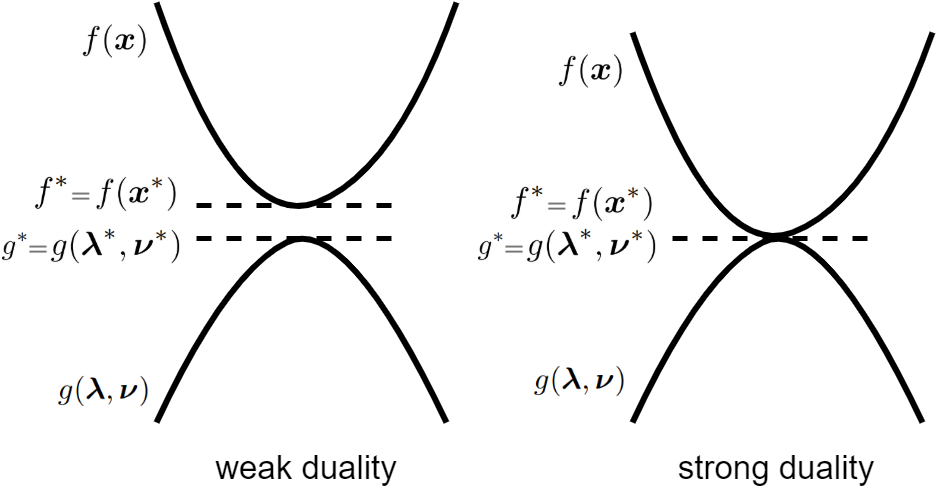
\includegraphics[width=3.2in]{./images/primal_dual_problems}
\caption{Illustration of weak duality and strong duality.}
\label{figure_primal_dual_problems}
\end{figure}

\begin{figure}[!t]
\centering
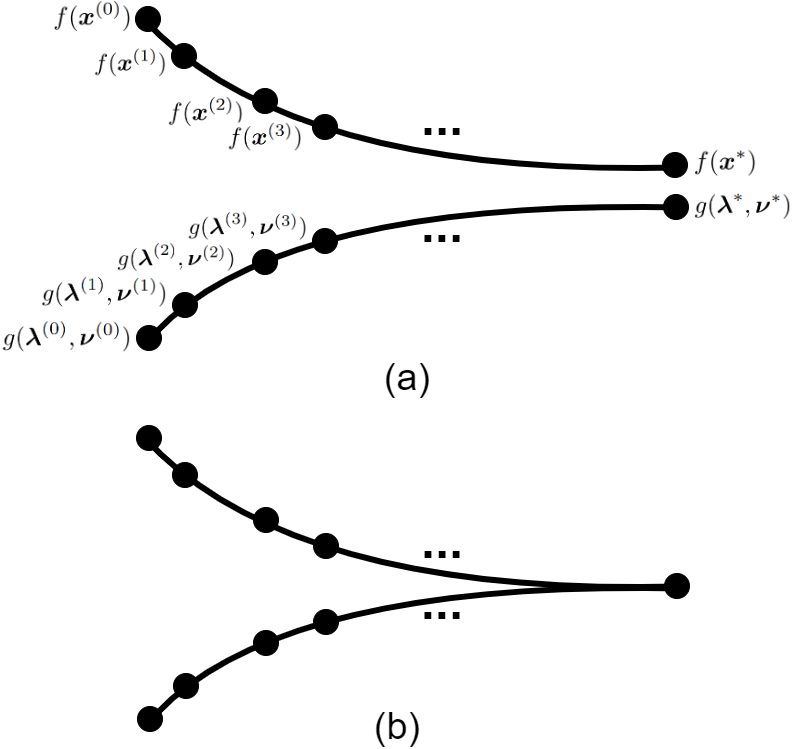
\includegraphics[width=3.2in]{./images/iterative_primal_dual}
\caption{Progress of iterative optimization: (a) gradual minimization of the primal function and maximization of dual function and (b) the primal optimal and dual optimal reach each other and become equal if strong duality holds.}
\label{figure_iterative_primal_dual}
\end{figure}

If optimization is iterative, the solution is updated iteratively until convergence. First-order and second-order numerical optimization, which we will introduce later, are iterative. 
In optimization, the series of primal optimal and dual optimal converge to the optimal solution and the dual optimal, respectively. The function values converge to the local minimum and the dual function values converge to the optimal (maximum) dual function. Let the superscript $(k)$ denotes the value of variable at iteration $k$. We have:
\begin{equation}\label{equation_iterative_optimization_series}
\begin{aligned}
& \{\boldsymbol{x}^{(0)}, \boldsymbol{x}^{(1)}, \boldsymbol{x}^{(2)}, \dots\} \rightarrow \boldsymbol{x}^*, \\
& \{\boldsymbol{\nu}^{(0)}, \boldsymbol{\nu}^{(1)}, \boldsymbol{\nu}^{(2)}, \dots\} \rightarrow \boldsymbol{\nu}^*, \\
& \{\boldsymbol{\lambda}^{(0)}, \boldsymbol{\lambda}^{(1)}, \boldsymbol{\lambda}^{(2)}, \dots\} \rightarrow \boldsymbol{\lambda}^*, \\
& f(\boldsymbol{x}^{(0)}) \geq f(\boldsymbol{x}^{(1)}) \geq f(\boldsymbol{x}^{(2)}) \geq \dots \geq f(\boldsymbol{x}^*), \\
& g(\boldsymbol{\lambda}^{(0)}, \boldsymbol{\nu}^{(0)}) \leq g(\boldsymbol{\lambda}^{(1)}, \boldsymbol{\nu}^{(1)}) \leq \dots \leq g(\boldsymbol{\lambda}^*, \boldsymbol{\nu}^*).
\end{aligned}
\end{equation}
Hence, the value of function goes down but the value of dual function goes up. As Fig. \ref{figure_iterative_primal_dual} depicts, they reach each other if strong duality holds; otherwise, there will be a gap between them after convergence.
Note that if the optimization problem is a convex problem, the eventually found solution is the global solution; otherwise, the solution is local. 

\begin{corollary}\label{corollary_dual_optimal_lower_bound_primal_optimal_iterative}
As every iteration of a numerical optimization must satisfy either the weak or strong duality, the optimum dual function at every iteration always provides a lower-bound for the optimum primal function at that iteration:
\begin{align}
g(\boldsymbol{\lambda}^{(k)}, \boldsymbol{\nu}^{(k)}) \leq f(\boldsymbol{x}^{(k)}), \quad \forall k.
\end{align}
\end{corollary}

\begin{lemma}[Slater's condition \cite{slater1950lagrange}]
For a convex optimization problem in the form: 
\begin{equation}\label{equation_optimization_problem_inequalityConstraints_Ax_equals_b_constraint}
\begin{aligned}
& \underset{\boldsymbol{x}}{\text{minimize}}
& & f(\boldsymbol{x}) \\
& \text{subject to}
& & y_i(\boldsymbol{x}) \leq 0, \; i \in \{1, \ldots, m_1\}, \\
& & & \boldsymbol{Ax} = \boldsymbol{b}, 
\end{aligned}
\end{equation}
we have strong duality if it is strictly feasible, i.e.:
\begin{equation}
\begin{aligned}
\exists \boldsymbol{x} \in \textbf{int}(\mathcal{D}):\, & y_i(\boldsymbol{x}) < 0, \quad \forall i \in \{1, \dots, m_1\}, \\
& \boldsymbol{Ax} = \boldsymbol{b}.
\end{aligned}
\end{equation}
In other words, for at least one point in the interior of domain (not on the boundary of domain), all the inequality constraints hold strictly. This is called the Slater's condition. 
\end{lemma}

\subsection{Complementary Slackness}

Assume that the problem has strong duality, the primal optimal is $\boldsymbol{x}^*$ and dual optimal variables are $\boldsymbol{\lambda}^*$ and $\boldsymbol{\nu}^*$. We have:
\begin{align}
f(\boldsymbol{x}^*) &\overset{(\ref{equation_strong_duality})}{=} g(\boldsymbol{\lambda}^*, \boldsymbol{\nu}^*) \nonumber \\
&\overset{(\ref{equation_dual_function})}{=} \inf_{\boldsymbol{x} \in \mathcal{D}} \Big(f(\boldsymbol{x}) + \sum_{i=1}^{m_1} \lambda_i^* y_i(\boldsymbol{x}) + \sum_{i=1}^{m_2} \nu_i^* h_i(\boldsymbol{x})\Big) \nonumber \\
&\overset{(a)}{=} f(\boldsymbol{x}^*) + \sum_{i=1}^{m_1} \lambda_i^* y_i(\boldsymbol{x}^*) + \sum_{i=1}^{m_2} \nu_i^* h_i(\boldsymbol{x}^*) \nonumber \\
&\overset{(b)}{=} f(\boldsymbol{x}^*) + \sum_{i=1}^{m_1} \lambda_i^* y_i(\boldsymbol{x}^*) \overset{(c)}{\leq} f(\boldsymbol{x}^*), \label{equation_complementary_slackness_step1}
\end{align}
where $(a)$ is because $\boldsymbol{x}^*$ is the primal optimal solution for problem (\ref{equation_optimization_problem}) and it minimizes the Lagrangian, $(b)$ is because $\boldsymbol{x}^*$ is a feasible point and satisfies $h_i(\boldsymbol{x}^*)=0$ in Eq. (\ref{equation_feasible_point}), and $(c)$ is because $\lambda_i^* \geq 0$ according to Eq. (\ref{equation_nonnegativity_dual_variables}) and the feasible $\boldsymbol{x}^*$ satisfies $y_i(\boldsymbol{x}^*) \leq 0$ in Eq. (\ref{equation_feasible_point}) so we have:
\begin{align}\label{equation_complementary_slackness_step2}
\lambda_i^* y_i(\boldsymbol{x}^*) \leq 0, \quad \forall i \in \{1, \dots, m_1\}.
\end{align}
From Eq. (\ref{equation_complementary_slackness_step1}), we have:
\begin{align*}
&f(\boldsymbol{x}^*) = f(\boldsymbol{x}^*) + \sum_{i=1}^{m_1} \lambda_i^* y_i(\boldsymbol{x}^*) \leq f(\boldsymbol{x}^*) \\
&\implies \sum_{i=1}^{m_1} \lambda_i^* y_i(\boldsymbol{x}^*) = 0 \overset{(\ref{equation_complementary_slackness_step2})}{\implies} \lambda_i^* y_i(\boldsymbol{x}^*) = 0, \forall i. 
\end{align*}
Therefore, the multiplication of every optimal dual variable $\lambda_i^*$ with $y_i(.)$ of optimal primal solution $\boldsymbol{x}^*$ must be zero. 
This is called the \textit{complementary slackness}:
\begin{align}
& \lambda_i^*\, y_i(\boldsymbol{x}^*) = 0, \quad \forall i \in \{1, \dots, m_1\}.
\end{align}
These conditions can be restated as:
\begin{align}
&\lambda_i^* > 0 \implies y_i(\boldsymbol{x}^*) = 0, \\
&y_i(\boldsymbol{x}^*) < 0 \implies \lambda_i^* = 0, 
\end{align}
which means that, for an inequality constraint, if the dual optimal is nonzero, its inequality function of the primal optimal must be zero. If the inequality function of the primal optimal is nonzero, its dual optimal must be zero.

% \subsection{Gradient Vanishing of Lagrangian}
\subsection{Stationarity Condition}

As was explained before, the Lagrangian function can be interpreted as a regularized cost function to be minimized. Hence, the constrained optimization problem (\ref{equation_optimization_problem}) is converted to minimization of the Lagrangian function, Eq. (\ref{equation_Lagrangian}), which is an unconstrained optimization problem:
\begin{align}
\underset{\boldsymbol{x}}{\text{minimize}}\,\, \mathcal{L}(\boldsymbol{x},\boldsymbol{\lambda},\boldsymbol{\nu}).
\end{align}
Note that this problem is the dual function according to Eq. (\ref{equation_dual_function}). 
As this is an unconstrained problem, its optimization is easy. We can find its minimum by setting its derivative w.r.t. $\boldsymbol{x}$, denoted by $\nabla_{\boldsymbol{x}} \mathcal{L}$, to zero:
\begin{equation}
\begin{aligned}
&\nabla_{\boldsymbol{x}} \mathcal{L}(\boldsymbol{x},\boldsymbol{\lambda},\boldsymbol{\nu}) = 0 \overset{(\ref{equation_Lagrangian})}{\implies} \\
& \nabla_{\boldsymbol{x}} f(\boldsymbol{x}) + \sum_{i=1}^{m_1} \lambda_i \nabla_{\boldsymbol{x}} y_i(\boldsymbol{x}) + \sum_{i=1}^{m_2} \nu_i \nabla_{\boldsymbol{x}} h_i(\boldsymbol{x}) = 0.
\end{aligned}
\end{equation}
This equation is called the \textit{stationarity condition} because this shows that the gradient of Lagrangian w.r.t. $\boldsymbol{x}$ should vanish to zero (n.b. a stationary point of a function is a point where the derivative of function is zero). This derivative holds for all dual variables and not just for the optimal dual variables. 
We can claim that the gradient of Lagrangian w.r.t. $\boldsymbol{x}$ should vanish to zero because the dual function, defined in Eq. (\ref{equation_dual_function}), should exist.  

\subsection{KKT Conditions}

We derived the primal feasibility, dual feasibility, complementary slackness, and stationarity condition. These four conditions are called the \textit{Karush-Kuhn-Tucker (KKT) conditions} \cite{karush1939minima,kuhn1951nonlinear}. 
The primal optimal variable $\boldsymbol{x}^*$ and the dual optimal variables $\boldsymbol{\lambda}^* = [\lambda_1^*, \dots, \lambda_{m_1}^*]^\top$, $\boldsymbol{\nu}^* = [\nu_1^*, \dots, \nu_{m_2}^*]^\top$ must satisfy the KKT conditions. 
We summarize the KKT conditions in the following: 
\begin{enumerate}
\item Stationarity condition:
\begin{equation}\label{equation_stationarity_condition}
\begin{aligned}
\nabla_{\boldsymbol{x}} \mathcal{L}(\boldsymbol{x},\boldsymbol{\lambda},\boldsymbol{\nu}) = &\nabla_{\boldsymbol{x}} f(\boldsymbol{x}) + \sum_{i=1}^{m_1} \lambda_i \nabla_{\boldsymbol{x}} y_i(\boldsymbol{x}) \\
&+ \sum_{i=1}^{m_2} \nu_i \nabla_{\boldsymbol{x}} h_i(\boldsymbol{x}) = 0.
\end{aligned}
\end{equation}
\item Primal feasibility:
\begin{align}
& y_i(\boldsymbol{x}^*) \leq 0, \quad \forall i \in \{1, \ldots, m_1\}, \\
& h_i(\boldsymbol{x}^*) = 0, \quad \forall i \in \{1, \ldots, m_2\}.
\end{align}
\item Dual feasibility:
\begin{align}\label{equation_dual_constraints}
\boldsymbol{\lambda} \succeq \boldsymbol{0} \quad\text{ or }\quad \lambda_i \geq 0, \,\, \forall i \in \{1, \dots, m_1\}.
\end{align}
\item Complementary slackness:
\begin{align}
\lambda_i^*\, y_i(\boldsymbol{x}^*) = 0, \quad \forall i \in \{1, \dots, m_1\}.
\end{align}
\end{enumerate}
As listed above, KKT conditions impose constraints on the optimal dual variables of inequality constraints because the sign of inequalities are important. 

Recall the dual problem (\ref{equation_dual_optimization_problem}). The constraint in this problem is already satisfied by the dual feasibility in the KKT conditions. Hence, we can ignore the constraint of the dual problem (as it is automatically satisfied by dual feasibility):
\begin{equation}\label{equation_dual_optimization_problem_unconstrained}
\begin{aligned}
& \underset{\boldsymbol{\lambda}, \boldsymbol{\nu}}{\text{maximize}}
& & g(\boldsymbol{\lambda}, \boldsymbol{\nu}), 
\end{aligned}
\end{equation}
which should give us $\boldsymbol{\lambda}^*$, $\boldsymbol{\nu}^*$, and $g^* = g(\boldsymbol{\lambda}^*, \boldsymbol{\nu}^*)$.
This is an unconstrained optimization problem and for solving it, we should set the derivative of $g(\boldsymbol{\lambda}, \boldsymbol{\nu})$ w.r.t. $\boldsymbol{\lambda}$ and $\boldsymbol{\nu}$ to zero:
\begin{align}
& \nabla_{\boldsymbol{\lambda}} g(\boldsymbol{\lambda}, \boldsymbol{\nu}) = 0 \overset{(\ref{equation_dual_function_2})}{\implies} \nabla_{\boldsymbol{\lambda}} \mathcal{L}(\boldsymbol{x}^*,\boldsymbol{\lambda},\boldsymbol{\nu}) = 0. \label{equation_derivative_Lagrangian_wrt_lambda_zero} \\
& \nabla_{\boldsymbol{\nu}} g(\boldsymbol{\lambda}, \boldsymbol{\nu}) = 0 \overset{(\ref{equation_dual_function_2})}{\implies} \nabla_{\boldsymbol{\nu}} \mathcal{L}(\boldsymbol{x}^*,\boldsymbol{\lambda},\boldsymbol{\nu}) = 0. \label{equation_derivative_Lagrangian_wrt_nu_zero}
\end{align}
Note that setting the derivatives of Lagrangian w.r.t. dual variables always gives back the corresponding constraints in the primal optimization problem. 
Eqs. (\ref{equation_stationarity_condition}), (\ref{equation_derivative_Lagrangian_wrt_lambda_zero}), and (\ref{equation_derivative_Lagrangian_wrt_nu_zero}) state that the primal and dual residuals must be zero. 

Finally, Eqs. (\ref{equation_dual_function}) and (\ref{equation_dual_optimization_problem_unconstrained}) can be summarized into the following max-min optimization problem:
\begin{align}
\sup_{\boldsymbol{\lambda}, \boldsymbol{\nu}}\, g(\boldsymbol{\lambda}, \boldsymbol{\nu}) \overset{(\ref{equation_dual_function})}{=} \sup_{\boldsymbol{\lambda}, \boldsymbol{\nu}}\, \inf_{\boldsymbol{x}}\, \mathcal{L}(\boldsymbol{x},\boldsymbol{\lambda}, \boldsymbol{\nu}) = \mathcal{L}(\boldsymbol{x}^*,\boldsymbol{\lambda}^*, \boldsymbol{\nu}^*).
\end{align}

The reason for the name KKT is as follows \cite{kjeldsen2000contextualized}. In 1952, Kuhn and Tucker published an important paper proposing the conditions \cite{kuhn1951nonlinear}. However, later it was found out that there is a master's these by Karush, in 1939, at the University of Chicago, Illinois \cite{karush1939minima}. That thesis had also proposed the conditions; however, researchers including Kuhn and Tucker were not aware of that thesis. Therefore, these conditions were named after all three of them. 

\subsection{Solving Optimization by Method of Lagrange Multipliers}\label{section_method_of_multipliers}

We can solve the optimization problem (\ref{equation_optimization_problem}) using duality and KKT conditions. 
This technique is also called the \textit{method of Lagrange multipliers}. 
For this, we should do the following steps:
\begin{enumerate}
\item We write the Lagrangian as Eq. (\ref{equation_Lagrangian}).
\item We consider the dual function defined in Eq. (\ref{equation_dual_function}) and we solve it: 
\begin{align}\label{equation_KKT_x_dagger}
\boldsymbol{x}^\dagger := \arg \min_{\boldsymbol{x}}\, \mathcal{L}(\boldsymbol{x},\boldsymbol{\lambda},\boldsymbol{\nu}). 
\end{align}
It is an unconstrained problem and according to Eqs. (\ref{equation_dual_function}) and (\ref{equation_stationarity_condition}), we solve this problem by taking the derivative of Lagrangian w.r.t. $\boldsymbol{x}$ and setting it to zero, i.e., $\nabla_{\boldsymbol{x}}\mathcal{L}(\boldsymbol{x},\boldsymbol{\lambda},\boldsymbol{\nu}) \overset{\text{set}}{=} 0$.
This gives us the dual function, according to Eq. (\ref{equation_Lagrangian}):
\begin{align}
g(\boldsymbol{\lambda}, \boldsymbol{\nu}) = \mathcal{L}(\boldsymbol{x}^\dagger,\boldsymbol{\lambda},\boldsymbol{\nu}). 
\end{align}

\item We consider the dual problem, defined in Eq. (\ref{equation_dual_optimization_problem}) which is simplified to Eq. (\ref{equation_dual_optimization_problem_unconstrained}) because of Eq. (\ref{equation_dual_constraints}). This gives us the optimal dual variables $\boldsymbol{\lambda}^*$ and $\boldsymbol{\nu}^*$:
\begin{align}
\boldsymbol{\lambda}^*, \boldsymbol{\nu}^* := \arg \max_{\boldsymbol{\lambda}, \boldsymbol{\nu}}\, g(\boldsymbol{\lambda},\boldsymbol{\nu}). 
\end{align}
It is an unconstrained problem and according to Eqs. (\ref{equation_derivative_Lagrangian_wrt_lambda_zero}) and (\ref{equation_derivative_Lagrangian_wrt_nu_zero}), we solve this problem by taking the derivative of dual function w.r.t. $\boldsymbol{\lambda}$ and $\boldsymbol{\nu}$ and setting them to zero, i.e., $\nabla_{\boldsymbol{\lambda}}g(\boldsymbol{\lambda},\boldsymbol{\nu}) \overset{\text{set}}{=} 0$ and $\nabla_{\boldsymbol{\nu}}g(\boldsymbol{\lambda},\boldsymbol{\nu}) \overset{\text{set}}{=} 0$.
The optimum dual value is obtained as:
\begin{align}
g^* = \max_{\boldsymbol{\lambda}, \boldsymbol{\nu}}\, g(\boldsymbol{\lambda},\boldsymbol{\nu}) = g(\boldsymbol{\lambda}^*,\boldsymbol{\nu}^*).
\end{align}
\item We put the optimal dual variables $\boldsymbol{\lambda}^*$ and $\boldsymbol{\nu}^*$ in Eq. (\ref{equation_stationarity_condition}) to find the optimal primal variable:
\begin{align}
\boldsymbol{x}^* := \arg \min_{\boldsymbol{x}}\, \mathcal{L}(\boldsymbol{x},\boldsymbol{\lambda}^*,\boldsymbol{\nu}^*). 
\end{align}
It is an unconstrained problem and we solve this problem by taking the derivative of Lagrangian at optimal dual variables w.r.t. $\boldsymbol{x}$ and setting it to zero, i.e., $\nabla_{\boldsymbol{x}}\mathcal{L}(\boldsymbol{x},\boldsymbol{\lambda}^*,\boldsymbol{\nu}^*) \overset{\text{set}}{=} 0$.
The optimum primal value is obtained as:
\begin{align}
f^* = \min_{\boldsymbol{x}}\, \mathcal{L}(\boldsymbol{x},\boldsymbol{\lambda}^*,\boldsymbol{\nu}^*) = \mathcal{L}(\boldsymbol{x}^*,\boldsymbol{\lambda}^*,\boldsymbol{\nu}^*).
\end{align}
\end{enumerate}

\section{First-Order Optimization: Gradient Methods}\label{section_first_order_methods}

\subsection{Gradient Descent}\label{section_gradient_descent}

\textit{Gradient descent} is one of the fundamental first-order methods. It was first suggested by Cauchy in 1874 \cite{lemarechal2012cauchy} and Hadamard in 1908 \cite{hadamard1908memoire} and its convergence was later analyzed in \cite{curry1944method}. In the following, we introduce this method. 

\subsubsection{Step of Update}\label{section_GD_step_update}

Consider the unconstrained optimization problem (\ref{equation_optimization_problem_unconstrained}).
Here, we denote $\boldsymbol{x}^* := \arg \min_{\boldsymbol{x}} f(\boldsymbol{x})$ and $f^* := \min_{\boldsymbol{x}} f(\boldsymbol{x}) = f(\boldsymbol{x}^*)$.
In numerical optimization for unconstrained optimization, we start with a random feasible initial point and iteratively update it by step $\Delta \boldsymbol{x}$: 
\begin{align}\label{equation_update_point_numerical_optimization}
\boldsymbol{x}^{(k+1)} := \boldsymbol{x}^{(k)} + \Delta \boldsymbol{x},
\end{align}
until we converge to (or get sufficiently close to) the desired optimal point $\boldsymbol{x}^*$. 
Note that the step $\Delta\boldsymbol{x}$ is also denoted by $\boldsymbol{p}$ in the literature, i.e., $\boldsymbol{p} := \Delta\boldsymbol{x}$.
Let the function $f(.)$ be differentiable and its gradient is $L$-smooth. 
If we set $\boldsymbol{x} = \boldsymbol{x}^{(k)}$ and $\boldsymbol{y} = \boldsymbol{x}^{(k+1)} = \boldsymbol{x}^{(k)} + \Delta \boldsymbol{x}$ in Eq. (\ref{equation_fundamental_theorem_calculus_Lipschitz}), we have:
\begin{align}
&f(\boldsymbol{x}^{(k)} + \Delta \boldsymbol{x}) \leq f(\boldsymbol{x}^{(k)}) + \nabla f(\boldsymbol{x}^{(k)})^\top \Delta \boldsymbol{x} + \frac{L}{2} \|\Delta \boldsymbol{x}\|_2^2 \nonumber\\
&\implies f(\boldsymbol{x}^{(k)} + \Delta \boldsymbol{x}) - f(\boldsymbol{x}^{(k)}) \nonumber\\
&~~~~~~~~~~~~~~~~~~~~~~~~~~~\leq \nabla f(\boldsymbol{x}^{(k)})^\top \Delta \boldsymbol{x} + \frac{L}{2} \|\Delta \boldsymbol{x}\|_2^2. \label{equation_fundamental_theorem_calculus_Lipschitz_GD}
\end{align}
Until reaching the minimum, we want to decrease the cost function $f(.)$ in every iteration; hence, we desire:
\begin{align}\label{equation_GD_decrease_cost_function}
f(\boldsymbol{x}^{(k)} + \Delta \boldsymbol{x}) - f(\boldsymbol{x}^{(k)}) < 0.
\end{align}
According to Eq. (\ref{equation_fundamental_theorem_calculus_Lipschitz_GD}), one way to achieve Eq. (\ref{equation_GD_decrease_cost_function}) is:
\begin{align*}
\nabla f(\boldsymbol{x}^{(k)})^\top \Delta \boldsymbol{x} + \frac{L}{2} \|\Delta \boldsymbol{x}\|_2^2 < 0.
\end{align*}
Hence, we should minimize $\nabla f(\boldsymbol{x}^{(k)})^\top \Delta \boldsymbol{x} + \frac{L}{2} \|\Delta \boldsymbol{x}\|_2^2$ w.r.t. $\Delta \boldsymbol{x}$:
\begin{align}\label{equation_GD_min_RHS_of_corollary_fundamental}
\underset{\Delta\boldsymbol{x}}{\text{minimize}}\,\, \nabla f(\boldsymbol{x}^{(k)})^\top \Delta \boldsymbol{x} + \frac{L}{2} \|\Delta \boldsymbol{x}\|_2^2.
\end{align}
This function is convex w.r.t. $\Delta \boldsymbol{x}$ and we can optimize it by setting its derivative to zero:
\begin{align}
&\frac{\partial }{\partial \Delta \boldsymbol{x}} (\nabla f(\boldsymbol{x}^{(k)})^\top \Delta \boldsymbol{x} + \frac{L}{2} \|\Delta \boldsymbol{x}\|_2^2) = \nabla f(\boldsymbol{x}^{(k)}) + L \Delta \boldsymbol{x} \nonumber\\
&\overset{\text{set}}{=} \boldsymbol{0} \implies \Delta \boldsymbol{x} = -\frac{1}{L} \nabla f(\boldsymbol{x}^{(k)}). \label{equation_GD_step_by_L}
\end{align}
Using Eq. (\ref{equation_GD_step_by_L}) in Eq. (\ref{equation_fundamental_theorem_calculus_Lipschitz_GD}) gives:
\begin{align*}
f(\boldsymbol{x}^{(k)} + \Delta \boldsymbol{x}) - f(\boldsymbol{x}^{(k)}) \leq -\frac{1}{2L} \|\nabla f(\boldsymbol{x}^{(k)})\|_2^2 \leq 0,
\end{align*}
which satisfies Eq. (\ref{equation_GD_decrease_cost_function}).
Eq. (\ref{equation_GD_step_by_L}) means that it is better to move toward a scale of minus gradient for updating the solution. This inspires the name of algorithm which is \textit{gradient descent}. 

The problem is that often we either do not know the Lipschitz constant $L$ or it is hard to compute. Hence, rather than Eq. (\ref{equation_GD_step_by_L}), we use:
\begin{align}\label{equation_GD_step_by_eta}
\Delta \boldsymbol{x} = -\eta \nabla f(\boldsymbol{x}^{(k)}), \text{ i.e., } \boldsymbol{x}^{(k+1)} := \boldsymbol{x}^{(k)} - \eta \nabla f(\boldsymbol{x}^{(k)}),
\end{align}
where $\eta > 0$ is the step size, also called the learning rate in data science literature. 
Note that if the optimization problem is maximization rather than minimization, the step should be $\Delta \boldsymbol{x} = \eta \nabla f(\boldsymbol{x}^{(k)})$ rather than Eq. (\ref{equation_GD_step_by_eta}). In that case, the name of method is \textit{gradient ascent}. 

Using Eq. (\ref{equation_GD_step_by_eta}) in Eq. (\ref{equation_fundamental_theorem_calculus_Lipschitz_GD}) gives:
\begin{align}
f(\boldsymbol{x}^{(k)} + \Delta \boldsymbol{x}) &- f(\boldsymbol{x}^{(k)}) \nonumber\\
&\leq -\eta \|\nabla f(\boldsymbol{x}^{(k)})\|_2^2 + \frac{L}{2} \eta^2 \|\nabla f(\boldsymbol{x}^{(k)})\|_2^2 \label{equation_GD_step_size_eta_L_mid1}\\
&= \eta (\frac{L}{2} \eta - 1) \|\nabla f(\boldsymbol{x}^{(k)})\|_2^2 \nonumber
\end{align}
If $\boldsymbol{x}^{(k)}$ is not a stationary point, we have $\|\nabla f(\boldsymbol{x}^{(k)})\|_2^2 > 0$. 
Noticing $\eta > 0$, for satisfying Eq. (\ref{equation_GD_decrease_cost_function}), we must set:
\begin{align}\label{equation_GD_step_size_eta_L}
\frac{L}{2} \eta - 1 < 0 \implies \eta < \frac{2}{L}.
\end{align}
On the other hand, we can minimize Eq. (\ref{equation_GD_step_size_eta_L_mid1}) by setting its derivative w.r.t. $\eta$ to zero:
\begin{align*}
&\frac{\partial }{\partial \eta} (-\eta \|\nabla f(\boldsymbol{x}^{(k)})\|_2^2 + \frac{L}{2} \eta^2 \|\nabla f(\boldsymbol{x}^{(k)})\|_2^2) \\
&= -\|\nabla f(\boldsymbol{x}^{(k)})\|_2^2 + L \eta \|\nabla f(\boldsymbol{x}^{(k)})\|_2^2 \\
&= (-1+L \eta) \|\nabla f(\boldsymbol{x}^{(k)})\|_2^2 \overset{\text{set}}{=} 0 \implies \eta = \frac{1}{L}.
\end{align*}
If we set:
\begin{align}\label{equation_GD_step_size_eta_L_2}
\eta < \frac{1}{L},
\end{align}
then Eq. (\ref{equation_GD_step_size_eta_L_mid1}) becomes:
\begin{align}
&f(\boldsymbol{x}^{(k)} + \Delta \boldsymbol{x}) - f(\boldsymbol{x}^{(k)}) \nonumber \\
&\leq -\frac{1}{L} \|\nabla f(\boldsymbol{x}^{(k)})\|_2^2 + \frac{1}{2L} \|\nabla f(\boldsymbol{x}^{(k)})\|_2^2 \nonumber \\
&= -\frac{1}{2L}\|\nabla f(\boldsymbol{x}^{(k)})\|_2^2 < 0 \nonumber \\
&\implies f(\boldsymbol{x}^{(k+1)}) \leq f(\boldsymbol{x}^{(k)}) -\frac{1}{2L}\|\nabla f(\boldsymbol{x}^{(k)})\|_2^2.
\label{equation_GD_decrease_cost}
\end{align}
Eq. (\ref{equation_GD_step_size_eta_L_2}) means that there should be an upper-bound, dependent on the Lipschitz constant, on the step size. Hence, $L$ is still required. 
Eq. (\ref{equation_GD_decrease_cost}) shows that every iteration of gradient descent decreases the cost function:
\begin{align}
f(\boldsymbol{x}^{(k+1)}) \leq f(\boldsymbol{x}^{(k)}),
\end{align}
and the amount of this decrease depends on the norm of gradient at that iteration. 
In conclusion, the series of solutions converges to the optimal solution while the function value decreases iteratively until the local minimum:
\begin{align*}
& \{\boldsymbol{x}^{(0)}, \boldsymbol{x}^{(1)}, \boldsymbol{x}^{(2)}, \dots\} \rightarrow \boldsymbol{x}^*, \\
& f(\boldsymbol{x}^{(0)}) \geq f(\boldsymbol{x}^{(1)}) \geq f(\boldsymbol{x}^{(2)}) \geq \dots \geq f(\boldsymbol{x}^*).
\end{align*}
If the optimization problem is a convex problem, the solution is the global solution; otherwise, the solution is local. 


\section{ADMM}


% \mainmatter
% \partsimage{1675670753831.jpg}
% \part{基础理论}
\chapterimage{wallhaven-d6g16l.jpg}
\chapter{\quad 计算学习理论}
\begin{center}
    \textcolor[RGB]{255, 0, 0}{\faHeart}世界以痛吻我,要我报之以歌.\textcolor[RGB]{255, 0, 0}{\faHeart}
\end{center}
\rightline{——泰戈尔}
\vspace{-5pt}
\begin{center}
    \pgfornament[width=0.36\linewidth,color=lsp]{88}
\end{center}

\begin{introduction}
  \item PAC学习定义
  \item 有限假设空间
  \item VC-维
  \item Rademacher复杂度
  \item 稳定性
\end{introduction}

\section{基础定义}

PAC学习理论即为概率近似正确(Probably Approximately Correct)学习理论. 通过PAC框架, 我们可以借助样本复杂度和空间复杂度来定义可学习类的概念. 首先, 给出如下定义.

将所有可能的\textbf{样本}(sample)或\textbf{实例}(instance)的集合记为$\mathcal{X}$ , 所有可能的\textbf{标签}(label)或\textbf{目标值}(target value)的集合用 $\mathcal{Y}$(其有时可为\textbf{输入空间})表示.  从最简单的\textbf{二分类}问题出发, 即$\mathcal{Y}=\{0,1\}$. 给定样本集 $D=\{(\mathbf{x}_i,y_i)\}_{i=1}^{m}$, $\mathbf{x}_i \in\mathcal{X}$.  假设 $\mathcal{X}$ 中的所有样本\textbf{独立同分布}(independent and identically distributed, $\textit{i.i.d.}$)于某个未知固定分布$\mathcal{D}$.  令$h$ 为从$\mathcal{X}$ 到 $\mathcal{Y}$的一个映射, 其\textbf{泛化误差}(generalization error)可表示为:
\begin{equation}
E\left( h; \mathcal{D} \right) =E\left( h \right) =  P_{\mathbf{x} \sim \mathcal{D} } \left( h\left( \mathbf{x} \right) \ne y \right)
\end{equation}
则$h$在$D$上的\textbf{经验误差}(empirical error)为:
\begin{equation}
\hat{E}\left( h;D \right) =\hat{E}\left( h \right)=\frac{1}{m}\sum_{i=1}^m{\mathbb{I}_{\left( h\left( \mathbf{x}_i \right) \ne y_i \right)}}
\end{equation}

因此, $h$ 的经验误差是其在样本集$D$上的平均误差, 而泛化误差则是其在分布$D$ 上误差的期望. 由于$D$ 为$\mathcal{D}$ 的独立同分布采样, 因此$h$的经验误差的期望等于其泛化误差.
\section{可学性}
对于一个\textbf{概念}(concept) $ c:\mathcal{X}\rightarrow \mathcal{Y}$ 为 $\mathcal{X}$ 到 $\mathcal{Y}$  的映射函数. 其表示了实例$\mathbf{x}$ 与其对应的标签或目标值$y$之间的真实关系, 对任意的$(\mathbf{x}_i,y_i)$ 都有$c(\mathbf{x}=y)$ 成立, 则称$c$ 为目标概念.  同时, 将所有希望学到的目标概念所构成的集合称为“概念类”(concept class), 记为$\mathcal{C}$. 给出如下定义: 

\begin{definition}[PAC学习]
若存在一个算法$\mathcal{A}$ 和一个多项式函数 $poly\left( \cdot ,\cdot ,\cdot ,\cdot \right)$ 使得任意 $\epsilon >0$和 $\delta >0$, 对所有在 $\mathcal{X}$ 上的分布 $\mathcal{D} $ 和任意的目标概念 $c\in\mathcal{C}$, 以及满足$m\ge poly\left( {1}/{\epsilon},{1}/{\delta},size(\mathbf{x}),size\left( c \right) \right) $ 的任意样本规模$m$ 均有下式成立, 那么概念类$\mathcal{C}$ 是PAC可学习的(PAC-learnable).
\begin{equation}
P\left( E\left( h \right) \le \epsilon \right) \ge 1-\delta
\end{equation}
进一步地, 若$\mathcal{A}$的运行复杂度在$poly\left( {1}/{\epsilon},{1}/{\delta},size(\mathbf{x}),size\left( c \right) \right) $ 内, 则概念类$\mathcal{C}$ 为高效PAC可学习的(efficiency PAC-learnable). 当这样的算法$\mathcal{A}$存在时, 则称该算法为$\mathcal{C}$ 的一个PAC学习算法(PAC-learning algorithm).
\end{definition}


PAC的定义可以理解为: 如果输入到一个算法的样本点数目对于${1}/{\epsilon}$ 和 ${1}/{\delta} $ 是多项式的, 并由该算法基于这些样本点得到的假设是以\textbf{高概率}(至少$1-\delta$)\textbf{近似正确}(误差至多$\epsilon$)的, 则概念类$\mathcal{C}$ 是PAC可学习的. 其中, $\delta>0$ 用来定义\textbf{置信程度}(confidence): $1-\delta$, $\epsilon >0$ 定义\textbf{准确性}(accuracy): $1-\epsilon$. 且对任意元素$\mathbf{x} \in \mathcal{X}$ 计算表示的代表的上界记为$size(\mathbf{x})$, 将对概念$c \in \mathcal{C}$计算表示的最大代价记为$size(c)$.

对于计算机算法而言, 其必然需要考虑时间复杂度,  假定学习算法$\mathcal{A}$处理每个样本的时间为常数, 则$\mathcal{A}$的时间复杂度等价于样本复杂度, 则可以给出样本复杂度的定义.  

\begin{definition}[样本复杂度]
满足PAC学习算法$\mathcal{A}$所需的 $m \ge poly ( {1}/{\epsilon},{1}/{\delta}, $
 $size(\mathbf{x}),size(c)) $ 中最小的$m$, 称为学习算法$\mathcal{A}$ 的样本复杂度(sample complexity).
\end{definition}

样本复杂度可以理解为评估算法学习概念类所需的样本规模. 定义2表明对算法$\mathcal{A}$而言, 如果学习算法的时间成本对于${1}/{\epsilon}$ 和 ${1}/{\delta} $ 是多项式的, 当算法输入为全部样本时, 其样本规模$m$ 也是多项式的.

PAC学习框架具有如下特点:
\begin{itemize}
  \item PAC学习框架是不依赖分布的模型(distribution-free model), 其对产生样本的分布$\mathcal{D}$并未做特别的假设.
  \item 大多数情形下, 使得泛化称为可能的必要条件是: 用于得到误差的训练样本与测试样本产生于相同的分布$\mathcal{D}$.
  \item PAC学习框架考虑的是概念类$\mathcal{C}$ 的可学习性, 而不是一个特殊概念的可学习性. (对于学习算法, 其概念类$\mathcal{C}$是已知的, 而目标概念$c \in \mathcal{C}$ 是未知的).
  \item 多数情况下, 尤其是对概念的计算表示无法精确表示时, 我们往往忽略PAC定义中关于$size(\mathbf{x})$和$size(c)$的多项式约束, 而只聚焦于样本复杂度.
\end{itemize}
\par
给定学习算法$\mathcal{A}$, 其所考虑的所有可能概念集合为“\textbf{假设空间}”(hypothesis space), 记为$\mathcal{H}$. 通常情形下, $\mathcal{H}$ 与 $\mathcal{C}$ 之间并不一致, 学习算法会将\textbf{自以为可能}的目标概念集中起来构成$\mathcal{H}$, 即$h\in\mathcal{H}$. 由于并不能确定$h$ 是否真是目标概念, 因此称其为“\textbf{假设}”(hypothesis). 则可得到如下两种情况:
\par
\begin{itemize}
  \item \textbf{一致}(consistent)情况: 若目标概念$c\in \mathcal{H}$, 则$\mathcal{H}$中存在假设可将所有实例按照与真实标签一致的方式完全分开, 则该问题对于学习算法$\mathcal{A}$是“可分的”(separable).
  \item \textbf{不一致}(inconsistent)情况: 若假设集中不包含目标概念, 即$c\ni \mathcal{H}$, 则$\mathcal{H}$中不存在假设可将所有实例按照与真实标签一致的方式完全分开, 则该问题对于学习算法$\mathcal{A}$是“不可分的”(non-separable).
\end{itemize}
\par
在此, 分别考虑假设空间$\mathcal{H}$ 有限时对应的\textbf{一致}和\textbf{不一致}情况.
\section{有限假设空间}
\subsection{一致情形}

在这一节, 我们在假设空间$\mathcal{H}$的势$|\mathcal{H}|$有限情况下, 且目标概念$c \in \mathcal{H}$时, 给出如下定理. 

\begin{theorem}[学习界\raisebox{0.5mm}{-----}有限$\mathcal{H}$, 一致情形)]
令 $\mathcal{H}$ 为由 $\mathcal{X}$ 到 $\mathcal{Y}$ 的映射函数组成的有限集合. 令 $\mathcal{A}$ 为学习任意目标概念 $c \in \mathcal{H}$ 的算法, 且依据独立同分布的样本集 $D$ 获得的是一个一致假设 h: $\hat{E}_D(h)=0$ . 则对于任意 $\epsilon,\delta >0$, 不等式  $P(\hat{E}_D(h)\le\epsilon)\ge 1-\delta $ 成立的条件是 :
\begin{equation}
m\ge \frac{1}{\epsilon}\left( \log \left| \mathcal{H} \right|+\log \frac{1}{\delta} \right)
\end{equation}
依据上式中的样本复杂度结果可以等价地得到如下泛化界, 对于任意  $\epsilon,\delta >0$ , 以至少 $1-\delta$ 的概率有
\begin{equation}
\hat{E}_D(h) \le \frac{1}{m}\left( \log \left| \mathcal{H} \right|+\log \frac{1}{\delta} \right)
\end{equation}
\end{theorem}

\begin{proof}
固定 $\epsilon>0$, 由于我们并不知道算法$\mathcal{A}$ 选择了哪一个一致性假设$h\in \mathcal{H}$, 其选择假设不仅与学习算法有关, 还与训练样本集$D$有关. 因此, 需要给出一个\textbf{一致收敛界}(uniform convergence bound), 即包括$h$ 在内对于由所有一致的假设构成集合均成立的界. 我们对某些一致假设 $h\in \mathcal{H}$ 误差大于 $\epsilon $ 的概率给出其对应的界. 对任意 $\epsilon>0$ , 定义 $ \mathcal{H}_\epsilon$ 为  $ \mathcal{H}_\epsilon = \left\{h\in\mathcal{H}:\hat{E}_D(h)>\epsilon \right\} $ . 在独立同分布的训练样本 $D$ 上,  $\mathcal{H}_\epsilon$ 中的假设 $h$ 的概率一致, 其上界可以限定为: \\
\begin{equation}
\mathbb{P}\left[ \hat{E}_D\left( h \right) =0 \right] \le \left( 1-\epsilon \right) ^m \nonumber
\end{equation}
通过对上界取并集, 可以得到:
\begin{equation}
\begin{aligned}
&\ \ \mathbb{P}\left[ \exists h\in \mathcal{H}_{\epsilon}:\hat{E}_D\left( h \right) =0 \right] =\mathbb{P}\left[ \hat{E}_D\left( h_1 \right) =0\lor \cdots \lor \hat{E}_D\left( h_{\left| \mathcal{H}_{\epsilon} \right|} \right) =0 \right] \\
& \le \sum_{h\in \mathcal{H}_{\epsilon}}{\mathbb{P}\left[ \hat{E}_D\left( h \right) =0 \right]}\le \sum_{h\in \mathcal{H}_{\epsilon}}{\left( 1-\epsilon \right) ^m} \ \ \ (\text{联合上界}) \\
& \le \left| \mathcal{H} \right|\left( 1-\epsilon \right) ^m\le \left| \mathcal{H} \right|e^{-m\epsilon} \nonumber
\end{aligned}
\end{equation}
其中, 最后一个不等式是基于$1-x \le e^{-x}$ 得到的, 令上式不大于$\delta$, 即$\left| \mathcal{H} \right|e^{-m\epsilon}\le \delta$. 可得:
\begin{equation}
m\ge \frac{1}{\epsilon}\left( \log \left| \mathcal{H} \right|+\log \frac{1}{\delta} \right) \nonumber
\end{equation}
定理得证.
\end{proof}
\par
该定理表明, 有限假设集情形下, 样本复杂度依赖于关于$1/\epsilon$ 和$1/\delta$的多项式, 一致算法$\mathcal{A}$ 是PAC学习算法. 且由式(5) 可知, 一致假设的泛化误差以一个随样本规模$m$的增加而减少的项为上界. 说明在给定更大规模的带标签训练样本时学习算法将获得更大的受益. 同时, 泛化误差减少的速率为 $\mathcal{O}(\frac{1}{m})$, 其上界随着$|\mathcal{H}|$的增加而增加,这说明假设集规模越大,学习就越困难. 但是其增长速率为对数型,其可以解释为表示 $\mathcal{H}$ 所需要的二进制位数. 因此上述定理保证了泛化误差由二进制表示位数 $log_2|\mathcal{H}|$和样本规模 $m$ 控制.

\subsection{不一致情形}
在更一般的情形下, 当假设集 $\mathcal{H}$ 中不存在与训练样本完全一致的假设, 即 $c \notin \mathcal{H}$.  事实上, 这在实际中更加典型和普遍, 其中的学习问题可能十分困难或概念类比学习算法使用的假设集更加复杂.  然而,  在训练样本上产生少量误差的不一致假设也可能是有用的, 且这种假设在一定条件下是可以保证学习效果的.\par
首先, 为了在更一般的情况下保证学习效果, 我们将使用 Hoeffding's 不等式或如下的推论,它将单一假设的泛化误差与经验误差联系起来. \\
\begin{theorem}[Hoeffding 不等式]\label{thm:Hoeffding}
令 $X_1$, $X_2$,..., $X_m$ 是独立的随机变量, 对任意 $i \in [1,m]$, $X_i$取值为$[a_i,b_i]$. 对任意 $\epsilon>0$ ,令 $S_m=\sum_{i=1}^m{X_i}$, 则有以下不等式成立:
\begin{equation}
\mathbb{P}\left[ S_m-E\left[ S_m \right] \ge \epsilon \right] \le \exp \left\{ \frac{-2\epsilon ^2}{\sum\limits_{i=1}^m{\left( b_i-a_i \right) ^2}} \right\}
\end{equation}
\begin{equation}
\mathbb{P}\left[ S_m-E\left[ S_m \right] \le -\epsilon \right] \le \exp \left\{ \frac{-2\epsilon ^2}{\sum\limits_{i=1}^m{\left( b_i-a_i \right) ^2}} \right\}
\end{equation}
\end{theorem}


\begin{lemma}\label{lem:1}
固定 $\epsilon>0$ , 对任意假设 $h:\mathcal{X}\rightarrow \left\{ 0,1 \right\} $, 有以下不等式成立 :
\begin{equation}
\mathbb{P}\left[ \hat{E}\left( h \right) -E\left( h \right) \ge \epsilon \right] \le \exp \left( -2m\epsilon ^2 \right)
\end{equation}
\begin{equation}
\mathbb{P}\left[ \hat{E}\left( h \right) -E\left( h \right) \le -\epsilon \right] \le \exp \left( -2m\epsilon ^2 \right)
\end{equation}
根据联合约束, 可以进一步得到 :
\begin{equation}
\mathbb{P}\left[ \left| \hat{E}\left( h \right) -E\left( h \right) \right|\ge \epsilon \right] \le 2\exp \left( -2m\epsilon ^2 \right)
\end{equation}
\end{lemma}

\begin{proof}
依据定理\ref{thm:Hoeffding},令 $a=0,b=1$. 可得
\begin{equation}
\mathbb{P}\left[ \bar{X}-\mathbb{E}\left[ X \right] \ge \epsilon \right] \le \exp \left( -2m\epsilon ^2 \right)
\end{equation}
且 $\hat{E}\left( h \right) =\frac{1}{m}\sum_{i=1}^m{\mathbb{I}_{h\left( x_i \right) \ne c\left( x_i \right)}}$,代入上式可得
\begin{equation}
\mathbb{P}\left[ \hat{E}\left( h \right) -E\left( h \right) \ge \epsilon \right] \le \exp \left( -2m\epsilon ^2 \right) \nonumber
\end{equation}
同理可得
\begin{equation}
\mathbb{P}\left[ \hat{E}\left( h \right) -E\left( h \right) \le -\epsilon \right] \le \exp \left( -2m\epsilon ^2 \right) \nonumber
\end{equation}
根据联合界得到双边不等式
\begin{equation}
\mathbb{P}\left[ \left| \hat{E}\left( h \right) -E\left( h \right) \right|\ge \epsilon \right] \le 2\exp \left( -2m\epsilon ^2 \right) \nonumber
\end{equation}
即得证. 
\end{proof}


\begin{lemma}\label{lem:2}
若训练集$D$包含$m$个从分布$\mathcal{D}$上独立同分布采样而得到的样例, $0<\epsilon<1$, 则对任意$h\in \mathcal{H}$, 下式以至少$1-\delta$ 的概率成立:
\begin{equation}
\hat{E}\left( h \right)-\sqrt{\frac{\ln \left( 2/\delta \right)}{2m}}\le E(h)\le \hat{E}\left( h \right)+\sqrt{\frac{\ln \left( 2/\delta \right)}{2m}}
\end{equation}
\end{lemma}


引理\ref{lem:2}表明, 当样本规模$m$较大时, $h$的经验误差是其泛化误差的近似. 


\begin{theorem}\label{thm:2}
若$\mathcal{H}$为有限假设空间, $0<\delta<1$, 则对任意 $h\in \mathcal{H}$, 有
\begin{equation}
\mathbb{P}(|E(h)-\hat{E}(h)|\le\sqrt{\frac{\ln \left| \mathcal{H} \right|+\ln \left( 2/\delta \right)}{2m}})\ge 1-\delta
\end{equation}
\end{theorem}


\begin{proof}
 令$h_1,h_2,\cdots,h_{\left| \mathcal{H} \right|}$ 为假设空间$\mathcal{H}$中的假设, 有
\begin{equation}
\begin{aligned}
&\mathbb{P}\left( \exists h\in \mathcal{H}:\left| E\left( h \right) -\hat{E}\left( h \right) \right|>\epsilon \right) \\
&=\mathbb{P}\left( \left( \left| E\left( h_1 \right) -\hat{E}\left( h_1 \right) \right|>\epsilon \right) \lor \cdots \lor \left| E\left( h_{\left| \mathcal{H} \right|} \right) -\hat{E}\left( h_{\left| \mathcal{H} \right|} \right) \right|>\epsilon \right) \\
&\le \sum_{h\in \mathcal{H}}{\mathbb{P}\left( \left| E\left( h \right) -\hat{E}\left( h \right) \right|>\epsilon \right)} \nonumber
\end{aligned}
\end{equation}
由上式可得:
\begin{equation}
\sum_{h\in \mathcal{H}}{\mathbb{P}\left( \left| E\left( h \right) -\hat{E}\left( h \right) \right|>\epsilon \right)}\le 2\left| \mathcal{H} \right|\exp \left( -2m\epsilon ^2 \right)
\end{equation}
令上式右边等于$\delta$, 则定理得证.
\end{proof}

由定理\ref{thm:2}可以看出, 误差界需要在减少经验误差和控制假设集的势之间做权衡. 依据\textbf{奥卡姆剃刀原则}(Occam's Razor principle) :  如果其他方面相同, 一个简单的假设集效果会更好.

当$c\notin \mathcal{H}$时, 学习算法$\mathcal{A}$无法学到目标概念$c$ 的$\epsilon$近似, 但在给定假设空间$\mathcal{H}$时, 其中必存在一个泛化误差最小的假设, 可以将该假设的 $\epsilon$近似作为目标, 即在$\mathcal{H}$ 中泛化误差最小的假设$\textrm{arg\ min}_{h\in\mathcal{H} }E(h)$.

因此, 以此为目标将PAC学习推广至$c\notin \mathcal{H}$的情况, 称为"不可知学习(agnostic learning)", 进而给出如下定义. 


\begin{definition}[不可知PAC学习]
令$\mathcal{H}$为一个假设集. $\mathcal{A}$ 是一个不可知PAC学习算法的条件是: 存在一个多项式函数 $poly(\cdot,\cdot,\cdot,\cdot)$ 使得对于任意 $\epsilon>0$ 以及 $\delta > 0$, 对于所有在$\mathcal{X}\times\mathcal{Y} $上的分布$D$, 对于满足 $m\ge poly(1/\epsilon,1/\delta,size(\mathbf{x}),size(c))$ 的任意样本规模有下面的不等式成立:
\begin{equation}
P\left( E\left( h \right) -\min_{h'\in \mathcal{H}}E\left( h' \right) \le \epsilon \right) \ge 1-\delta
\end{equation}
进一步地, 若算法$\mathcal{A}$可在$poly(1/\epsilon,1/\delta,size(\mathbf{x}),size(c))$内执行, 则其可以被称为一个高效的不可知PAC学习算法.
\end{definition}


\section{VC-维和Rademacher复杂度}
\subsection{增长函数}
\noindent
\begin{definition}[增长函数]
假设空间$\mathcal{H}$的增长函数$\Pi _{\mathcal{H}}\left( m \right) : \mathbb{N}\rightarrow\mathbb{N} $,定义为:
\begin{equation}
\Pi _{\mathcal{H}}\left( m \right) =\max_{\left\{ \mathbf{x}_1,\cdots ,\mathbf{x}_m \right\} \subseteq \mathcal{H}}\left| \left\{ \left( h\left( \mathbf{x}_1 \right) ,\cdots ,h\left( \mathbf{x}_m \right) \right) \left| h\in \mathcal{H} \right. \right\} \right|,\ \forall m\in \mathbb{N}
\end{equation}
\end{definition}

\colorbox{yellow}{增长函数$\Pi _{\mathcal{H}}\left( m \right)$ 表示假设空间$\mathcal{H}$ 对$m$ 个样本所能赋予标记的最大可能结果数,} 也可以说是表示假设空间$\mathcal{H}$中的元素能够将$m$ 个点完成分类的最大方式数.这提供了一种新的衡量假设空间$\mathcal{H}$丰富度(表示能力)的方式, 且其并不依赖于样本分布, 而是一个纯粹的组合测量概念. 我们可以利用增长函数来估计经验误差与泛化误差之间的关系. \\
\begin{theorem}
对假设空间$\mathcal{H}$,$m\in \mathbb{N}$,$0<\epsilon<1$和任意$h\in\mathcal{H}$ 有:
\begin{equation}
\mathbb{P}\left( \left| E\left( h \right) -\hat{E}\left( h \right) \right|>\epsilon \right) \le 4\Pi _{\mathcal{H}}\left( 2m \right) \exp \left( -\frac{m\epsilon ^2}{8} \right)
\end{equation}
\end{theorem}

对二分类问题, $\mathcal{H}$中的假设对$D$中实例赋予标记的每种可能结果称为对$D$的一种“\textbf{对分}”(dichotomy).

若假设空间$\mathcal{H}$ 能实现实例集$D$上的所有对分, 即$\Pi _{\mathcal{H}}\left( 2m \right) = 2^m$, 则称实例集$D$能被假设空间$\mathcal{H}$ “\textbf{打散}”(shattering).

\subsection{VC-维}
VC维(Vapnik-Chervonenkis dimension)是对假设空间复杂度的度量, 其同样是一个纯粹的组合测量概念, 但其比增长函数更便于计算, 且与增长函数有直接联系. \\

\begin{definition}[VC-维]
一个假设集 $\mathcal{H}$ 的VC-维是指它能完全打散的最大集合的大小, 即
\begin{equation}
VC\left( \mathcal{H} \right) =\max\left\{ m:\Pi _{\mathcal{H}}\left( m \right) =2^m\right\}
\end{equation}
\end{definition}

$VC\left( \mathcal{H} \right) =d$表明存在大小为$d$的实例集可以被假设空间$\mathcal{H}$打散(但这并不意味着所有大小为$d$或小于$d$的集合都可以被完全打散). VC-维的定义与数据分布$\mathcal{D}$无关! 即使在数据分布未知时仍能计算得到假设空间$\mathcal{H}$的VC-维.

通常情况下, 若存在大小为$d$的实例集能被$\mathcal{H}$打散, 但不存在任何大小为$d+1$的实例集可以被$\mathcal{H}$打散, 则$\mathcal{H}$的VC维是$d$.

根据Sauer 引理, 可以看到增长函数与VC-维之间的联系. 

\begin{theorem}[Sauer 引理]\label{thm:Sauer}
若假设空间$\mathcal{H}$的VC-维为$d$, 则对任意$m\in \mathcal{N}$有
\begin{equation}
\Pi _{\mathcal{H}}\left( m \right) \le \sum_{i=0}^d{\left( \begin{array}{c}
	m\\
	i\\
\end{array} \right)}
\end{equation}
\end{theorem}

\begin{proof}
数学归纳法证明. 当$m=1,d=0$或$d=1$时, 定理成立. 假设上式对于$(m-1,d-1)$和$(m-1,d)$成立, 令$D=\left\{\mathbf{x}_1,\mathbf{x}_2,\cdots, \mathbf{x}_m\right\}$, $D'=\left\{\mathbf{x}_1,\mathbf{x}_2,\cdots, \mathbf{x}_{m-1}\right\}$, 则
\begin{eqnarray}
&\mathcal{H}_{\left| D \right.}=\left\{ \left( h\left( \mathbf{x}_1 \right) ,h\left( \mathbf{x}_2 \right) ,\cdots ,h\left( \mathbf{x}_m \right) \right) \left| h\in \mathcal{H} \right. \right\} \\
& \mathcal{H}_{\left| D' \right.}=\left\{ \left( h\left( \mathbf{x}_1 \right) ,h\left( \mathbf{x}_2 \right) ,\cdots ,h\left( \mathbf{x}_{m-1} \right) \right) \left| h\in \mathcal{H} \right. \right\}
\end{eqnarray}
任意假设$h\in\mathcal{H}$对$\mathbf{x}_m$的分类结果为$+1$或$-1$, 因此任意出现在$\mathcal{H}_{\left| D' \right.}$中的串(分类结果)都会在$\mathcal{H}_{\left| D \right.}$中出现一次至两次. 令$\mathcal{H}_{D'\left| D \right.}$表示在$\mathcal{H}_{\left| D \right.}$中出现两次的$\mathcal{H}_{\left| D' \right.}$中的串组成的集合, 即
\begin{eqnarray}
 \nonumber
\mathcal{H}_{D'\left| D \right.}=\left\{ \left( y_1,y_2,\cdots ,y_{m-1} \right) \in \mathcal{H}_{\left| D' \right.}\left| \exists h,h'\in \mathcal{H}, \right. \right.\\
\left. \left( h\left( \mathbf{x}_i \right) =h'\left( \mathbf{x}_i \right) =y_i \right) \land \left( h\left( \mathbf{x}_m \right) \ne h'\left( \mathbf{x}_m \right) \right) ,1\le i\le m-1 \right\}
\end{eqnarray}
考虑到$\mathcal{H}_{D'\left| D \right.}$中的串在$\mathcal{H}_{\left| D \right.}$中出现了两次, 但在$\mathcal{H}_{\left| D \right.}$中仅出现了一次, 有
\begin{equation}
\left| \mathcal{H}_{\left| D \right.} \right|=\left| \mathcal{H}_{\left| D' \right.} \right|+\left| \mathcal{H}_{D'\left| D \right.} \right|
\end{equation}
$D'$的大小为$m-1$,由假设可得
\begin{equation}
\left| \mathcal{H}_{\left| D' \right.} \right|\le \Pi _{\mathcal{H}}\left( m-1 \right) \le \sum_{i=0}^d{\left( \begin{array}{c}
	m-1\\
	i\\
\end{array} \right)}
\end{equation}
令$Q$表示能被$\mathcal{H}_{D'\left| D \right.} $打散的集合, 由$\mathcal{H}_{D'\left| D \right.} $定义可知$Q\cup \left\{ \mathbf{x}_m \right\} $ 必能被$\mathcal{H}_{\left| D \right.} $打散. 由于$\mathcal{H}$的VC-维为$d$, 因此, $\mathcal{H}_{D'\left| D \right.} $的VC-维最大为$d-1$,于是有:
\begin{equation}
\left| \mathcal{H}_{D'\left| D \right.} \right|\le \Pi _{\mathcal{H}}\left( m-1 \right) \le \sum_{i=0}^{d-1}{\left( \begin{array}{c}
	m-1\\
	i\\
\end{array} \right)}
\end{equation}
由式(23) $\sim$ (25)可得
\begin{eqnarray}
\begin{aligned}
 \nonumber
\left| \mathcal{H}_{\left| D \right.} \right|\le& \sum_{i=0}^d{\left( \begin{array}{c}
	m-1\\
	i\\
\end{array} \right) +\sum_{i=0}^{d-1}{\left( \begin{array}{c}
	m-1\\
	i\\
\end{array} \right)}} \\  \nonumber
=&\sum_{i=0}^d{\left( \left( \begin{array}{c}
	m-1\\
	i\\
\end{array} \right) +\left( \begin{array}{c}
	m-1\\
	i-1\\
\end{array} \right) \right)}\\ \nonumber
=&\sum_{i=0}^d{\left( \frac{\left( m-1 \right) !}{i!\left( m-i-1 \right) !}+\frac{\left( m-1 \right) !}{\left( i-1 \right) !\left( m-i \right) !} \right)}\\ \nonumber
=&\sum_{i=0}^d{\left( +\frac{\left( m-1 \right) !\left( m-i \right) +\left( m-1 \right) !i}{i!\left( m-i \right) !} \right)}\\  \nonumber
=&\sum_{i=0}^d{\left( \frac{m!}{i!\left( m-i \right) !} \right)}=\sum_{i=0}^d{\left( \begin{array}{c}
	m\\
	i\\
\end{array} \right)}  \nonumber
\end{aligned}
\end{eqnarray}
其中, $\left( \begin{array}{c} m-1\\ -1\\ \end{array} \right) =0$, 由于集合$D$是任意指定的, 故定理\ref{thm:Sauer}得证.  
\end{proof}


\begin{corollary}
若假设空间$\mathcal{H}$的VC-维为$d$, 则对任意整数$m\ge d$ 有:
\begin{equation}
\Pi _{\mathcal{H}}\left( m \right) \le \left( \frac{e\cdot m}{d} \right) ^d
\end{equation}
\end{corollary}

\begin{proof}
基于Sauer 引理,可以得到
\begin{eqnarray}
\begin{aligned}
\Pi _{\mathcal{H}}\left( m \right) &\le \sum_{i=0}^d{\left( \begin{array}{c}
	m\\
	i\\
\end{array} \right)}
\le \sum_{i=0}^d{\left( \begin{array}{c}
	m\\
	i\\
\end{array} \right)}\left( \begin{array}{c}
	m\\
	d\\
\end{array} \right) ^{d-i} \\
&=\left( \frac{m}{d} \right) ^d\sum_{i=0}^d{\left( \begin{array}{c}
	m\\
	i\\
\end{array} \right) \left( \frac{d}{m} \right)}^i
\le \left( \frac{m}{d} \right) ^d\sum_{i=0}^m{\left( \begin{array}{c}
	m\\
	i\\
\end{array} \right) \left( \frac{d}{m} \right)}^i \\
&=\left( \frac{m}{d} \right) ^d\left( 1+\frac{d}{m} \right) ^m
\le \left( \frac{e\cdot m}{d} \right) ^d
\end{aligned}
\end{eqnarray}
在运用二项式定理后, 依据不等式$(1-x)\le e^{-x}$,可以得到最终不等式.  
\end{proof}

\begin{theorem}\label{thm:5}
若假设空间$\mathcal{H}$的VC-维为$d$, 则对任意$m>d,0<\delta<1$和$h\in \mathcal{H}$有
\begin{equation}
\mathbb{P}\left( \left| E\left( h \right) -\hat{E}\left( h \right) \right|\le \sqrt{\frac{8d\ln \frac{2em}{d}+8\ln \frac{4}{\delta}}{m}} \right) \ge 1-\delta
\end{equation}
\end{theorem}

\begin{proof}
令$4\Pi _{\mathcal{H}}\left( 2m \right) \exp \left( -\frac{m\epsilon ^2}{8} \right) \le 4\left( \frac{2em}{d} \right) ^d\exp \left( -\frac{m\epsilon ^2}{8} \right) =\delta$, 解得
\begin{equation}
\epsilon =\sqrt{\frac{8d\ln \frac{2em}{d}+8\ln \frac{4}{\delta}}{m}}
\end{equation}
代入定理3即得证.
\end{proof}

定理\ref{thm:5}说明, 式(28)的泛化误差只与实例规模$m$有关, 与数据分布$\mathcal{D}$和实例集$D$无关, 且其收敛速率为$O\left( \frac{1}{\sqrt{m}} \right)$. 因此, 基于VC-维的泛化误差界是\textbf{分布无关}(distribution-free)且\textbf{数据独立}(data-independent)的.

\subsection{Rademacher复杂度}
Rademacher复杂度是另一种刻画假设空间复杂度的途径, 其通过衡量一个假设集拟合随机噪声的程度, 来捕获假设空间(函数族)的丰富度. 与VC-维不同, 其在一定程度上考虑了数据分布. 

\begin{definition}\label{def:6}
考虑实值函数空间$\mathcal{F}:\mathcal{Z}\rightarrow \mathbb{R}$, 令$Z = \left\{\boldsymbol{z}_1,\boldsymbol{z}_2,\cdots,\boldsymbol{z}_m\right\}$且其样本规模固定为$m$, 其中, $\boldsymbol{z}_i \in \mathcal{Z}$. 则函数空间$\mathcal{F}$关于$Z$的经验Rademacher复杂度为:
\begin{equation}
\hat{R}_Z\left( \mathcal{F} \right) =\mathbb{E}_{\boldsymbol{\sigma }}\left[ \underset{f\in \mathcal{F}}{sup}\frac{1}{m}\sum_{i=1}^m{\sigma _if\left( \boldsymbol{z}_i \right)} \right]
\end{equation}
其中$\boldsymbol{\sigma }=\left\{\sigma_1,\sigma_2,\cdots,\sigma_m\right\}$, $\sigma_i$为独立同分布的随机向量, 其称作Rademacher变量. 
\end{definition}

经验Rademacher复杂度衡量了函数空间$\mathcal{F}$与随机噪声在集合$Z$中的相关性. 为了了解函数空间$\mathcal{F}$在$\mathcal{Z}$上关于分布$\mathcal{D}$的相关性. 因此, 给出如下定义. 

\begin{definition}\label{def:7}
对所有从$\mathcal{D}$独立同分布采样而得到的大小为$m$的集合$Z$, 函数空间$\mathcal{F}$ 关于$\mathcal{Z}$上分布$\mathcal{D}$的Rademacher复杂度 :
\begin{equation}
R_m\left( \mathcal{F} \right) =\mathbb{E}_{Z\subseteq \mathcal{Z}:\left| Z \right|=m}\left[ \hat{R}_Z\left( \mathcal{F} \right) \right]
\end{equation}
\end{definition}

基于Rademacher复杂度可得到关于$\mathcal{F}$的泛化误差界. 

\begin{theorem}\label{thm:6}
对实值函数空间$\mathcal{F}: \mathcal{Z}\rightarrow [0,1]$, 根据分布$\mathcal{D}$从$\mathcal{Z}$中独立同分布采样得到示例集$Z=\left\{\boldsymbol{z}_1,\boldsymbol{z}_2,\cdots,\boldsymbol{z}_m\right\}$, $\boldsymbol{z}_i\in \mathcal{Z}$, $0<\delta<1$, 对任意$f\in \mathcal{F}$, 所以至少$1-\delta$的概率有:
\begin{eqnarray}
\begin{aligned}
\mathbb{E}\left[ f\left( \boldsymbol{z} \right) \right] &\le \frac{1}{m}\sum_{i=1}^m{f\left( \boldsymbol{z}_i \right)}+2R_m\left( \mathcal{F} \right) +\sqrt{\frac{\ln \left( 1/\delta \right)}{2m}},\\
\mathbb{E}\left[ f\left( \boldsymbol{z} \right) \right] &\le \frac{1}{m}\sum_{i=1}^m{f\left( \boldsymbol{z}_i \right)}+2\hat{R}_Z\left( \mathcal{F} \right) +3\sqrt{\frac{\ln \left( 1/\delta \right)}{2m}}
\end{aligned}
\end{eqnarray}
\end{theorem}

\begin{proof}
令
\begin{eqnarray}
\begin{aligned}
\hat{E}_Z\left( f \right) =& \frac{1}{m}\sum_{i=1}^m{f\left( \boldsymbol{z}_i \right)} \\
\Phi \left( Z \right) =& \underset{f\in \mathcal{F}}{\text{sup}}\mathbb{E}\left[ f \right] -\hat{E}_Z\left( f \right)
\end{aligned}
\end{eqnarray}
同时, 令$Z'$为只与$Z$有一个示例不同的训练集, 不妨设$\mathbf{z}_m\in Z$和$\mathbf{z}_{m}^{'}\in Z'$为不同示例, 可得\\
\begin{equation}
\begin{aligned}
\Phi \left( Z' \right) -\Phi \left( Z \right) =&\left( \underset{f\in \mathcal{F}}{\text{sup}}\mathbb{E}\left[ f \right] -\hat{E}_{Z'}\left( f \right) \right) -\left( \underset{f\in \mathcal{F}}{\text{sup}}\mathbb{E}\left[ f \right] -\hat{E}_Z\left( f \right) \right) \\
=&\underset{f\in \mathcal{F}}{\text{sup}}\hat{E}_Z\left( f \right) -\hat{E}_{Z'}\left( f \right)  \\
=&\underset{f\in \mathcal{F}}{\text{sup}}\frac{f\left( \boldsymbol{z}_m \right) -f\left( \boldsymbol{z}_{m}^{'} \right)}{m}\le \frac{1}{m}
\end{aligned}
\end{equation}
同理可得
\begin{eqnarray}
\Phi \left( Z \right) -\Phi \left( Z' \right) \le \frac{1}{m} \\
\left| \Phi \left( Z \right) -\Phi \left( Z' \right) \right|\le \frac{1}{m}
\end{eqnarray}
在此引入McDiarmid不等式. \\
\textcolor[rgb]{0.5,0.3,0.2}{\textbf{McDiarmid不等式}: 若$x_1,x_2,...,x_m$ 为$m$个独立随机变量, 且对任意$1\le i\le m$, 函数$f$满足
\begin{equation}
\underset{x_1,...,x_m,x_{i}^{'}}{\text{sup}}\left| f\left( x_1,...,x_m \right) -f\left( x_1,...,x_{i-1},x_{i}^{'},x_{i+1},...,x_m \right) \right|\le c_i.
\end{equation}}
\textcolor[rgb]{0.5,0.3,0.2}{则对任意$\epsilon >0$,有
\begin{eqnarray}
&P\left( f\left( x_1,...,x_m \right) -\mathbb{E}\left( f\left( x_1,...,x_m \right) \right) \ge \epsilon \right) \le \exp \left( \frac{-2\epsilon ^2}{\sum\limits_i^{}{c_{i}^{2}}} \right) \\
&P\left( \left| f\left( x_1,...,x_m \right) -\mathbb{E}\left( f\left( x_1,...,x_m \right) \right) \right|\ge \epsilon \right) \le 2\exp \left( \frac{-2\epsilon ^2}{\sum\limits_i^{}{c_{i}^{2}}} \right)
\end{eqnarray}}
将$\varPhi$看作是(38)中的函数$f$则有
\begin{equation}
P\left(  \varPhi \left( Z \right) -\mathbb{E}_Z\left[ \varPhi \left( Z \right) \right] \ge \epsilon \right) \le \exp \left( \frac{-2\epsilon ^2}{\sum\limits_i^{}{c_{i}^{2}}} \right) \nonumber
\end{equation}
令$\exp \left( \frac{-2\epsilon ^2}{\varSigma _ic_{i}^{2}} \right) =\delta  $可以求得$\epsilon =\sqrt{\frac{\ln \left( 1/\delta \right)}{2m}}$,所以
\begin{equation}
P\left( \varPhi \left( Z \right) -\mathbb{E}_Z\left[ \varPhi \left( Z \right) \right] \ge \sqrt{\frac{\ln \left( 1/\delta \right)}{2m}} \right) \le \delta
\end{equation}
由逆事件的概率定义得
\begin{equation}
P\left( \varPhi \left( Z \right) -\mathbb{E}_Z\left[ \varPhi \left( Z \right) \right] \le \sqrt{\frac{\ln \left( 1/\delta \right)}{2m}} \right) \ge 1-\delta
\end{equation}
下面来估计$\mathbb{E}_Z\left[ \varPhi \left( Z \right) \right] $的上界,有
\begin{equation}
\begin{aligned}
\mathbb{E}_Z\left[ \varPhi \left( Z \right) \right] &=\mathbb{E}_Z\left[ \underset{f\in \mathcal{F}}{\text{sup}}\left( \mathbb{E}\left[ f \right] -\hat{E}_Z\left( f \right) \right) \right] \\
&=\mathbb{E}_Z\left[ \underset{f\in \mathcal{F}}{\text{sup}}\mathbb{E}_{Z'}\left[ \hat{E}_{Z'}\left( f \right) -\hat{E}_Z\left( f \right) \right] \right] \\
&\le \mathbb{E}_{Z,Z'}\left[ \underset{f\in \mathcal{F}}{\text{sup}}\left( \hat{E}_{Z'}\left( f \right) -\hat{E}_Z\left( f \right) \right) \right]\\
&=\mathbb{E}_{Z,Z'}\left[ \underset{f\in \mathcal{F}}{\text{sup}}\frac{1}{m}\sum_{i=1}^m{\left( f\left( \boldsymbol{z}_{i}^{'} \right) -f\left( \boldsymbol{z}_i \right) \right)} \right]\\
&= \mathbb{E}_{\boldsymbol{\sigma },Z,Z'}\left[ \underset{f\in \mathcal{F}}{\text{sup}}\frac{1}{m}\sum_{i=1}^m{\sigma _i\left( f\left( \boldsymbol{z_{i}^{'}} \right) -f\left( \boldsymbol{z}_i \right) \right)} \right]\\
&\le  \mathbb{E}_{\boldsymbol{\sigma},Z'}\left[ \underset{f\in \mathcal{F}}{\text{sup}}\frac{1}{m}\sum_{i=1}^m{\sigma _if\left( \boldsymbol{z}_{i}^{'} \right)} \right] +\mathbb{E}_{\boldsymbol{\sigma},Z}\left[ \underset{f\in \mathcal{F}}{\text{sup}}\frac{1}{m}\sum_{i=1}^m{-\sigma _if\left( \boldsymbol{z}_i \right)} \right]\\
&= 2\mathbb{E}_{\boldsymbol{\sigma},Z}\left[ \underset{f\in \mathcal{F}}{\text{sup}}\frac{1}{m}\sum_{i=1}^m{\sigma _if\left( \boldsymbol{z}_i \right)} \right]\\
&= 2R_m\left( \mathcal{F} \right)
\end{aligned}
\end{equation}
\par
\begin{itemize}
  \item (42)$\rightarrow$(43)是在外面套了一个对服从分布$\mathcal{D}$的实例集$Z'$求期望. 且因为$\mathbb{E}_{Z'\thicksim \mathcal{D}}\left[ \hat{E}_{Z'}\left( f \right) \right] =\mathbb{E}\left[ f \right] $, 而采样出来的$Z'$和$Z$相互独立, 则有$\mathbb{E}_{Z'\thicksim \mathcal{D}}\left[ \hat{E}_{Z'}\left( f \right) \right] =\hat{E}\left[ f \right] $.
  \item (43)$\rightarrow$(44)的不等式基于上确界函数sup是凸函数, 根据Jesen不等式\\
  \textcolor{red}{
 \textbf{ Jesen不等式}\ \ 对任意凸函数$f(x)$,有
  \begin{equation}
  f\left( \mathbb{E}\left( x \right) \right) \le \mathbb{E}\left( f\left( x \right) \right)
  \end{equation}
  }
  则有
  \begin{equation}
  \mathbb{E}_Z\left[ \underset{f\in \mathcal{F}}{\text{sup}}\mathbb{E}_{Z'}\left[ \hat{E}_{Z'}\left( f \right) -\hat{E}_Z\left( f \right) \right] \right] \le \mathbb{E}_{Z,Z'}\left[ \underset{f\in \mathcal{F}}{\text{sup}}\left( \hat{E}_{Z'}\left( f \right) -\hat{E}_Z\left( f \right) \right) \right]
  \end{equation}
  其中$\mathbb{E}_{Z,Z'}$是$\mathbb{E}_Z\left[ \mathbb{E}_{Z'}\left[ \cdot \right] \right] $ 的简写形式.
  \item (45)$\rightarrow$(46)  则引入对Rademacher随机变量的期望, 由于函数值空间为标量, 而$\sigma_i$也是标量, 即$\sigma_i \in \{-1,+1\}$, 且$\sigma_i$总可以以相同概率取到这两个值, 因此可以引入$\mathbb{E}_{\sigma}$而不影响最终结果.
  \item (46)$\rightarrow$(47)是因为上确界之和不小于和的上确界. 同时, 因为第一项中只含有变量$\mathbf{z}'$, 则可以去掉$\mathbb{E}_{\boldsymbol{\sigma}}$; 而第二项中只含变量$\mathbf{z}$所以可以去掉$\mathbb{E}_{Z'}$.
  \item (47)$\rightarrow$(48)利用了$\boldsymbol{\sigma}$的对称性(即$-\boldsymbol{\sigma}$的分布与$\boldsymbol{\sigma}$完全一致)去除了第二项中的负号, 又因为$Z$和$Z'$均是从$\mathcal{D}$中独立同分布采样得到的数据, 因此可以将第一项中的$\mathbf{z}_{i}^{'}$替换成$\mathbf{z}$, 将$Z'$替换成$Z$, 最后根据式(31)可得$\mathbb{E}_Z\left[ \varPhi \left( Z \right) \right] =2\mathcal{R}_m\left( \mathcal{F} \right) $, 式得证.
\end{itemize}
\end{proof}

定理\ref{thm:6}给出了基于Rademacher复杂度的泛化误差界. 而关于Rademacher复杂度与增长函数, 有如下定理: 

\begin{theorem}\label{thm:7}
假设空间$\mathcal{H}$的Rademacher复杂度$R_m\left(\mathcal{H}\right)$与增长函数 $\Pi _{\mathcal{H}}\left( m \right) $满足
\begin{equation}
R_m\left( \mathcal{H} \right) \le \sqrt{\frac{2\ln \Pi _{\mathcal{H}}\left( m \right)}{m}}
\end{equation}
\end{theorem}

由式\textrm{(27)}和\textrm{(52)}以及推论(3)可得

\begin{equation}
E\left( h \right) \le \hat{E}\left( h \right) +\sqrt{\frac{2d\ln \frac{em}{d}}{m}}+\sqrt{\frac{\ln \left( \dfrac{1}{\delta} \right)}{2m}}
\end{equation}
因此, 可以从Rademacher复杂度和增长函数推导出基于VC维的泛化误差界.


\section{稳定性}
无论是基于VC维还是Rademacher复杂度来推导泛化误差界, 所得到的结果均与具体学习算法无关, 且对所有学习算法都适用. 但若希望获得与算法有关的分析结果, 则需要采取另外的指标来进行评价和衡量, \textbf{稳定性}就是一个指标, 其考察的是在算法输入发生变化时, 输出是否会随之发生较大的变化. 学习算法的输入即训练集, 其变化可以分为以下两种.
\par
给定$D=\left\{ \boldsymbol{z}_1=\left( \boldsymbol{x}_1,y_1 \right) ,\cdots ,\boldsymbol{z}_m=\left\{ \boldsymbol{x}_m,y_m \right\} \right\} $, $\boldsymbol{x}_i\in \mathcal{X}$来自分布$\mathcal{D}$的独立同分布示例, 且$y_i\in \left\{ -1,+1 \right\} $. 对假设空间$\mathcal{H}:\mathcal{X}\rightarrow \left\{ -1,+1 \right\} $和学习算法$\mathfrak{L}$, 令$\mathfrak{L}_D\in \mathcal{H}$表示基于训练集$D$从假设空间$\mathcal{H}$中学到的假设,则$D$存在如下两种变化:
\begin{itemize}
  \item $D^{\backslash i}$表示移除$D$中第$i$个样例得到的集合: \\
  \begin{equation}
  D^{\backslash i}=\left\{ \boldsymbol{z}_1,\boldsymbol{z}_2,...,\boldsymbol{z}_{i-1},\boldsymbol{z}_{i+1},...,\boldsymbol{z}_m \right\}
  \end{equation}
  \item $D^{ i}$表示替换$D$中第$i$个样例得到的集合: \\
\begin{equation}
  D^{ i}=\left\{ \boldsymbol{z}_1,\boldsymbol{z}_2,...,\boldsymbol{z}_{i-1},\boldsymbol{z}_{i-1}^{'},\boldsymbol{z}_{i+1},...,\boldsymbol{z}_m \right\}
  \end{equation}
\end{itemize}
其中,$\boldsymbol{z}_{i}^{'}=\left( \boldsymbol{x}_{i}^{'},y_{i}^{'} \right) $, $ \boldsymbol{x}_{i}^{'}$服从分布$\mathcal{D}$并独立于$D$.
\par
损失函数$\ell \left( \mathfrak{L}_D\left( \boldsymbol{x} \right) ,y \right) :\mathcal{Y}\times \mathcal{Y}\rightarrow \mathbb{R}^+ $刻画了假设$\mathfrak{L}_D$的预测标记$\mathfrak{L}_D\left( \boldsymbol{x} \right)$与真实标记$y$之间的差别, 并简记为$\ell \left( \mathfrak{L}_D,\boldsymbol{z}\right) $. 定义关于假设$\mathfrak{L}_D$的几种损失.
\begin{itemize}
  \item 泛化损失\\
\begin{equation}
\ell \left( \mathfrak{L}\ ,\mathcal{D} \right) =\mathbb{E}_{x\in \mathcal{X},\boldsymbol{z}=\left( \boldsymbol{x,}y \right)}\left[ \ell \left( \mathfrak{L}_D,\boldsymbol{z} \right) \right]
  \end{equation}
  \item 经验损失\\
  \begin{equation}
  \hat{\ell}\left( \mathfrak{L}, D \right) =\frac{1}{m}\sum_{i=1}^m{\ell \left( \mathfrak{L}_D,\boldsymbol{z}_i \right)}
  \end{equation}
  \item 留一(leave-one-out)损失 \\
  \begin{equation}
\hat{\ell}\left( \mathfrak{L}, D \right) =\frac{1}{m}\sum_{i=1}^m{\ell \left( \mathfrak{L}_{D^{\backslash i}},\boldsymbol{z}_i \right)}
  \end{equation}
\end{itemize}


\begin{definition}[均匀稳定性(uniform stability)] 
对任何$x\in \mathcal{X},\ \boldsymbol{z}=\left( \boldsymbol{x,}y \right) $. 若学习算法满足
\begin{equation}
\left| \ell \left( \mathfrak{L}_D,\boldsymbol{z} \right) -\ell \left( \mathfrak{L}_{D^{\backslash i}},\boldsymbol{z}_i \right)\right|\le \beta ,i=1,2,...,m,
\end{equation}
则称$\mathfrak{L}$关于损失函数$\ell$满足$\beta$-均匀稳定性.  \textcolor{red}{ (少一个数据,损失变化较小)}
\end{definition}

若算法$\mathfrak{L}$关于损失函数$\ell$满足$\beta$-均匀稳定性, 则:

\begin{equation}
\begin{aligned}
&\left| \ell \left( \mathfrak{L}_D,\boldsymbol{z} \right) -\ell \left( \mathcal{L}_{D^i},\boldsymbol{z} \right) \right| \\
\le &\left| \ell \left( \mathfrak{L}_D,\boldsymbol{z} \right) -\ell \left( \mathfrak{L}_{D^{\backslash i}},\boldsymbol{z} \right) \right|+\left| \ell \left( \mathfrak{L}_{D^i},\boldsymbol{z} \right) -\ell \left( \mathfrak{L}_{D^{\backslash i}},\boldsymbol{z} \right) \right|\\
\le &  2\beta ,
\end{aligned}
\end{equation}
移除示例的稳定性包含替换示例的稳定性. 
\begin{theorem}\label{thm:8}
若损失函数$\ell$有界, 即对所有$D$和$\boldsymbol{z}=\left( \boldsymbol{x}, y \right) $ 有$0\le \ell \left( \mathfrak{L}_D,\boldsymbol{z} \right) \le M$. 给定从分布$\mathcal{D}$上独立同分布采样得到的大小为$m$的示例集$D$, 若学习算法$\mathfrak{L}$满足关于损失函数$\ell$的$\beta$-均匀稳定性, 且$\ell$的上界为$M$, $0<\delta<1$, 则对任意$m\ge 1$, 以至少$1-\delta$的概率有
\begin{equation}
\ell \left( \mathfrak{L},\mathcal{D} \right) \le \hat{\ell}\left( \mathfrak{L},D \right) +2\beta +\left( 4m\beta +M \right) \sqrt{\frac{\ln \left( \dfrac{1}{\delta} \right)}{2m}},
\end{equation}

\begin{equation}
 \ell \left( \mathfrak{L},\mathcal{D} \right) \le \ell _{loo}\left( \mathfrak{L},D \right) +\beta +\left( 4m\beta +M \right) \sqrt{\frac{\ln \left( \dfrac{1}{\delta} \right)}{2m}}.
\end{equation}
由(61)得: 经验损失与泛化误差之间差别的收敛为$\beta \sqrt{m}$, 若$\beta =\mathcal{O}\left( \frac{1}{m} \right) $, 则可保证收敛率为$\mathcal{O}\left( \frac{1}{m} \right)$. 
\end{theorem}

\begin{itemize}
  \item \textcolor{red}{学习算法稳定性分析关注的是: \ $\left| \hat{\ell}\left( \mathfrak{L},D \right) -\ell \left( \mathfrak{L},\mathcal{D} \right) \right|$.}
 \item \textcolor{red}{假设空间复杂度分析关注的是: \ $\text{sup}_{h\in \mathcal{H}}\left| \widehat{E}\left( h \right) -E\left( h \right) \right|$.}
\end{itemize}


稳定性分析不必考虑假设空间中所有可能的假设, 只需根据算法自身的特性(稳定性)来讨论输出假设$\mathfrak{L}_D$的泛化误差界. 则稳定性与可学习性之间何种关系?
\par
假设$\beta \sqrt{m}\rightarrow 0$, 保证稳定的学习算法$\mathfrak{L}$具有一定的泛化能力, 即经验损失收敛于泛化损失. 假定$\beta =\frac{1}{m}$, 代入式(1.61)可得
\begin{equation}
\ell \left( \mathfrak{L},\mathcal{D} \right) \le \hat{\ell}\left( \mathfrak{L},\mathcal{D} \right) +\frac{2}{m}+\left( 4+M \right) \sqrt{\frac{\ln \left( \dfrac{1}{\delta} \right)}{2m}}
\end{equation}
对于损失函数$\ell$, 若学习算法$\mathfrak{L}$所输出的假设满足经验损失最小化, 称算法$\mathfrak{L}$满足经验风险最小化(Emprical Risk Minimization)原则. 简称算法是ERM的. 且存在如下定理: 

\begin{theorem}\label{thm:9}
 若学习算法$\mathfrak{L}$是ERM且稳定的, 则假设空间$\mathcal{H}$可学习. 
 \end{theorem}
 
 \textcolor{blue}{ 学习算法的稳定性能导出假设空间的科学性, 稳定性与假设空间并非无关, 由稳定性的定义可知两者通过损失函数$\ell$联系起来. }
 
\begin{proof}
令$g$表示$\mathcal{H}$中具有最小泛化损失的假设, 即
 \begin{equation}
 \ell \left( g,\mathcal{D} \right) =\min_{h\in \mathcal{H}}\ell \left( h,\mathcal{D} \right) .
 \end{equation}
 再令
\begin{equation}
  \epsilon '=\frac{\epsilon}{2} \nonumber
\end{equation}
\begin{equation}
  \frac{\delta}{2}=2\exp \left( -2m\left( \epsilon ' \right) ^2 \right) \nonumber
\end{equation}
将$\epsilon '=\frac{\epsilon}{2}$代入$\frac{\delta}{2}=2\exp \left( -2m\left( \epsilon ' \right) ^2 \right)$可以解得$m=\frac{2}{\epsilon ^2}\ln \frac{4}{\delta}$, 由Hoeffding不等式, 有
\begin{equation}
P\left( \left| \frac{1}{m}\sum_{i=1}^m{x_i}-\frac{1}{m}\sum_{i=1}^m{\mathbb{E}\left( x_i \right)} \right|\ge \epsilon \right) \le 2\exp \left( -2m\epsilon ^2 \right)
\end{equation}
其中$\frac{1}{m}\sum\limits_{i=1}^m{\mathbb{E}\left( x_i \right) =\ell \left( g,\mathcal{D} \right)}$, $\frac{1}{m}\sum\limits_{i=1}^m{x_i=\hat{\ell}\left( g,\mathcal{D} \right)}$, 代入可得
\begin{equation}
P\left( \left| \ell \left( g,\mathcal{D} \right) -\hat{\ell}\left( g,D \right) \right|\ge \frac{\epsilon}{2} \right) \le \frac{\delta}{2}
\end{equation}
根据逆事件的概率可得
\begin{equation}
P\left( \left| \ell \left( g,\mathcal{D} \right) -\hat{\ell}\left( g,D \right) \right|\le \frac{\epsilon}{2} \right) \ge 1- \frac{\delta}{2}
\end{equation}
令式(1.63)中
\begin{equation}
\frac{2}{m}+\left( 4+M \right) \sqrt{\frac{\ln \left( \dfrac{2}{\delta} \right)}{2m}}=\frac{\epsilon}{2}
\end{equation}
可以求解出
\begin{equation}
\sqrt{m}=\frac{\left( 4+M \right) \sqrt{\frac{\ln \left( \dfrac{2}{\delta} \right)}{2}}+\sqrt{\left( 4+M \right) ^2\cdot \frac{\ln \left( \dfrac{2}{\delta} \right)}{2}-4\cdot \frac{\epsilon}{2}\cdot \left( -2 \right)}}{2\cdot \frac{\epsilon}{2}}
\end{equation}
则有$m=\mathcal{O}\left( \frac{1}{\epsilon ^2}\ln \frac{1}{\delta} \right) $使
\begin{equation}
\ell \left( \mathfrak{L},\mathcal{D} \right) \le \hat{\ell}\left( \mathfrak{L},D \right) +\frac{\epsilon}{2}
\end{equation}
以至少$1-\dfrac{1}{\delta}$的概率成立, 从而可得
\begin{equation}
\begin{aligned}
\ell \left( \mathfrak{L},\mathcal{D} \right) -\ell \left( g,\mathcal{D} \right) &\le \hat{\ell}\left( \mathfrak{L},D \right) +\frac{\epsilon}{2}-\left( \hat{\ell}\left( g,D \right) -\frac{\epsilon}{2} \right)\\
&\le \hat{\ell}\left( \mathfrak{L},D \right) -\hat{\ell}\left( g,D \right) +\epsilon \\
& \le \epsilon
\end{aligned}
\end{equation}
以至少$1-\delta$的概率成立, 定理9得证.
\end{proof}

\mainmatter
\partsimage{1675670753831.jpg}
\part{线性模型}
\chapterimage{wallhaven-9d6g28.jpg}
\chapter{\quad 线性模型}
\vspace{0.5in}
	\begin{center}
	    \textcolor[RGB]{255, 0, 0}{\faHeart}真正能带来满足感的不是苗条或财富, 而是肯定自己的人生.\textcolor[RGB]{255, 0, 0}{\faHeart}
	\end{center}
	\rightline{——《心流: 最优体验心理学》}
%\begin{center}
%    \includegraphics{线性分类.png}
%\end{center}
\begin{center}
    \pgfornament[width=0.36\linewidth,color=lsp]{88}
\end{center}
\section{基本线性模型}
线性模型即通过样本特征的线性组合来进行预测的模型. 

给定数据集$D=\left\{ \left( \boldsymbol{x}_i,y_i \right) \right\} _{i=1}^{n}$. 其中, $\boldsymbol{x}_i$ $=\left[ \boldsymbol{x}_{i1},\boldsymbol{x}_{i2},...,\boldsymbol{x}_{im} \right] ^T$ , $y_i\in \mathbb{R}$ . 回归(Regression)问题就是基于输入属性(特征) $\boldsymbol{x}$来尽可能准确地预测实值输出$y$. 线性回归试图学得如下模型:
\begin{equation}
f\left( \boldsymbol{x}_i \right) =\boldsymbol{w}^T\boldsymbol{x}_i+b
\end{equation}
其中, $\boldsymbol{w}$和$b$分别为系数向量和截距(偏置). 

\subsection{最小二乘线性回归}
最小二乘回归采用均方误差 (Mean Square Error,MSE) (即$\ell_2$范数定义的平方误差)作为损失函数,那么损失函数就是关于变量$\boldsymbol{w}$和$b$的函数:
\begin{equation}
\begin{aligned}
L\left( \boldsymbol{\hat{w}} \right) =\sum_{i=1}^n{\lVert \boldsymbol{\hat{w}}^T\!\boldsymbol{x}_i-y_i \rVert _{2}^{2}}&=\left[ \boldsymbol{\hat{w}}^T\!\boldsymbol{x}_1-y_1,\cdots ,\boldsymbol{\hat{w}}^T\!\boldsymbol{x}_n-y_n \right] \left[ \begin{array}{c}
	\boldsymbol{\hat{w}}^T\!\boldsymbol{x}_1-y_1\\
	\vdots\\
	\boldsymbol{\hat{w}}^T\!\boldsymbol{x}_n-y_n\\
\end{array} \right] \\
&=\left( \mathbf{X}\boldsymbol{\hat{w}}-\mathbf{y} \right) ^T\left( \mathbf{X}\boldsymbol{\hat{w}}-\mathbf{y} \right)
\end{aligned}
\end{equation}
其中 $\boldsymbol{\hat{w}}= [\boldsymbol{w}; b]$. 相应的数据集的输入矩阵也表示为$\mathbf{X}\in \mathbb{R}^{n\times (m+1)}$, 则
\begin{equation}
\mathbf{X}=\left[ \begin{matrix}
	x_{11}&		x_{12}&		\cdots&		x_{1m}&		1\\
	x_{21}&		x_{22}&		\cdots&		x_{2m}&		1\\
	\vdots&		\vdots&		\ddots&		\vdots&		\vdots\\
	x_{n1}&		x_{n2}&		\cdots&		x_{nm}&		1\\
\end{matrix} \right] =\left[ \begin{matrix}
	\boldsymbol{x}_{1}^{T}&		1\\
	\boldsymbol{x}_{2}^{T}&		1\\
	\vdots&		\vdots\\
	\boldsymbol{x}_{n}^{T}&		1\\
\end{matrix} \right]  \nonumber
\end{equation}
则输出可以表示成$\mathbf{y}=[y_1,y_2,...,y_n]^T$. 通过最小化$\boldsymbol{\hat{w}}$, 有:
\begin{equation}
\begin{aligned}
\boldsymbol{\hat{w}} = argmin_{\boldsymbol{\hat{w}}}L\left( \boldsymbol{\hat{w}} \right) &\rightarrow \frac{\partial L\left( \boldsymbol{\hat{w}} \right)}{\partial \boldsymbol{\hat{w}}}=0\\
&\rightarrow 2\mathbf{X}^T\mathbf{X}\boldsymbol{\hat{w}}-2\mathbf{X}^T\mathbf{y}=0 \\
& \rightarrow \boldsymbol{\hat{w}}=\left( \mathbf{X}^T\mathbf{X} \right) ^{-1}\mathbf{X}^T\mathbf{y}=\mathbf{X}^{\dag}\mathbf{y}
\end{aligned}
\end{equation}
则最终学习得到的多元线性回归模型为:
\begin{equation}
f\left( \boldsymbol{\hat{x}}_i \right) =\boldsymbol{\hat{x}}_{i}^{T}\left( \mathbf{X}^T\mathbf{X} \right) ^{-1}\mathbf{X}^T\mathbf{y}
\end{equation}
其中, $X^{\dag} = (\mathbf{X}^T\mathbf{X} )^{-1}\mathbf{X}^T$为矩阵$\mathbf{X} $的伪逆.  当$\mathbf{X} $为行满秩或列满秩时可以直接求解, 但是对于非满秩的样本集合$\mathbf{X} $ 则需要通过奇异值分解(SVD), 得到

\begin{equation}
\mathbf{X}=\mathbf{U\Sigma V}^T
\end{equation}
于是:
\begin{equation}
\mathbf{X}^{\dag}=\mathbf{V\Sigma }^{-1}\mathbf{U}^T
\end{equation}
从几何的角度, 最小二乘法相当于模型和样本间的距离平方求和, 假设我们的训练样本张成一个$n$维空间(满秩情况): $\mathbf{X}=Span\left( \boldsymbol{x}_1,\boldsymbol{x}_2,\cdots ,\boldsymbol{x}_n \right) $. 而模型可以写成$f\left( \boldsymbol{w} \right) =\mathbf{X}\boldsymbol{w}$, 即$\boldsymbol{x}_1,\boldsymbol{x}_2,\cdots ,\boldsymbol{x}_n$的某种组合, 而最小二乘法希望$\mathbf{y}$与模型的误差或距离越小越好, 于是它们的差应该与这个张成的空间垂直:
\begin{equation}
\mathbf{X}^T\left( \mathbf{y}-\mathbf{X}\boldsymbol{\beta } \right) =0\rightarrow \boldsymbol{w }=\left( \mathbf{X}^T\mathbf{X} \right) ^{-1}\mathbf{X}^T\mathbf{y}
\end{equation}
同时, 若$\mathbf{X}^T\mathbf{X}$的逆存在, 我们也可以将$\boldsymbol{w}$表示为如下形式:
\begin{equation}
\boldsymbol{w}=\left( \mathbf{X}^T\mathbf{X} \right) ^{-1}\mathbf{X}^T\mathbf{y}=\mathbf{X}^T\mathbf{X}\left( \mathbf{X}^T\mathbf{X} \right) ^{-2}\mathbf{X}^T\mathbf{y}=\mathbf{X}^T\boldsymbol{\alpha } \label{con:lincom}
\end{equation}
可以看出, 公式\eqref{con:lincom}说明系数向量$\boldsymbol{w}$可以表示为训练样本的线性组合, 即$\boldsymbol{w}=\sum_{i=1}^n{\alpha _i\boldsymbol{x}_i}$.
%\subsection{Gauss-Markov定理}
%当参数$\theta$的数学期望等于其真实的未知参数时, 即$E\left\{ \hat{\theta} \right\} =\theta $,称参数$\theta$的估计$\hat{\theta}$为无偏估计. 进一步地,如果无偏估计还具有最小方差,则称其为最优无偏估计。对数据向量$\bm{b}$含有加性噪声或扰动的方程$\boldsymbol{A\theta }=\boldsymbol{b}+\boldsymbol{e}$, 若最小二乘解$$





\subsection{噪声为高斯分布的MLE}
记$y=\boldsymbol{w}^T\boldsymbol{x}+\epsilon ,\epsilon \thicksim N\left( 0,\sigma ^2 \right) $, 那么$y\thicksim N\left( \boldsymbol{w}^T\boldsymbol{x,}\sigma ^2 \right) $. 代入极大似然估计中:
\begin{equation}
\begin{aligned}
L\left( \boldsymbol{w} \right) &=\log p\left( \mathbf{y}\left| \mathbf{X},\boldsymbol{w} \right. \right) =\log \prod_{i=1}^n{p\left( y_i\left| \boldsymbol{x}_i,\boldsymbol{w} \right. \right)}\\
&=\sum_{i=1}^n{\log \left( \frac{1}{\sqrt{2\pi \sigma}}e-\frac{\left( y_i-\boldsymbol{w}^T\boldsymbol{x}_i \right) ^2}{2\sigma ^2} \right)}\\
argmax_{\boldsymbol{w}}L\left( \boldsymbol{w} \right) &=argmax_{\boldsymbol{w}}\sum_{i=1}^n{\left( y_i-\boldsymbol{w}^T\boldsymbol{x}_i \right) ^2}
\end{aligned}
\end{equation}
其最终的结果与最小二乘估计的结果一致. 
\section{贝叶斯线性回归}
当线性回归当噪声为高斯分布的时候, 最小二乘损失导出的结果相当于对概率模型应用 MLE, 引入参数的先验时, 先验分布是高斯分布, 那么 MAP的结果相当于岭回归的正则化; 如果先验是拉普拉斯分布, 那么相当于 Lasso 的正则化. 这两种方案都是点估计方法, 我们希望利用贝叶斯方法来求解参数的后验分布. 线性回归的模型假设为:
\begin{equation}
\begin{array}{c}
f(x)=w^{T} x \\
y=f(x)+\varepsilon \\
\varepsilon \sim \mathcal{N}\left(0, \sigma^{2}\right)
\end{array}
\end{equation}
在贝叶斯方法中, 需要解决推断和预测两个问题. 
\subsection{推断}
引入高斯先验: $p(w)=\mathcal{N}(0,\Sigma_p)$. 对参数的后验分布进行推断: 
\begin{equation}
p(w \mid X, Y)=\frac{p(w, Y \mid X)}{p(Y \mid X)}=\frac{p(Y \mid w, X) p(w \mid X)}{\int p(Y \mid w, X) p(w \mid X) d w}
\end{equation}
分母和参数无关, 由于 $p(w|X)=p(w)$, 代入先验得到: 
\begin{equation}
p(w \mid X, Y) \propto \prod_{i=1}^{N} \mathcal{N}\left(y_{i} \mid w^{T} x_{i}, \sigma^{2}\right) \cdot \mathcal{N}\left(0, \Sigma_{p}\right)
\end{equation}
高斯分布取高斯先验的共轭分布依然是高斯分布, 于是可以得到后验分布也是一个高斯分布. 第一项: 
\begin{equation}
\begin{aligned}
\prod_{i=1}^{N} \mathcal{N}\left(y_{i} \mid w^{T} x_{i}, \sigma^{2}\right) & =\frac{1}{(2 \pi)^{N / 2} \sigma^{N}} \exp \left(-\frac{1}{2 \sigma^{2}} \sum_{i=1}^{N}\left(y_{i}-w^{T} x_{i}\right)^{2}\right) \\
& =\frac{1}{(2 \pi)^{N / 2} \sigma^{N}} \exp \left(-\frac{1}{2}(Y-X w)^{T}\left(\sigma^{-2} \mathbb{I}\right)(Y-X w)\right) \\
& =\mathcal{N}\left(X w, \sigma^{2} \mathbb{I}\right)
\end{aligned}
\end{equation}
代入上面的式子:
\begin{equation}
p(w \mid X, Y) \propto \exp \left(-\frac{1}{2 \sigma^{2}}(Y-X w)^{T} \sigma^{-2} \mathbb{I}(Y-X w)-\frac{1}{2} w^{T} \Sigma_{p}^{-1} w\right)
\end{equation}
假定最后得到的高斯分布为: $\mathcal{N}(\mu_w,\Sigma_w)$. 对于上面的分布, 采用配方的方式来得到最终的分布, 指数上面的二次项为$-\frac{1}{2 \sigma^{2}} w^{T} X^{T} X w-\frac{1}{2} w^{T} \Sigma_{p}^{-1} w$. 于是有:
\begin{equation}
\Sigma_{w}^{-1}=\sigma^{-2} X^{T} X+\Sigma_{p}^{-1}=A
\end{equation}
一次项: 
\begin{equation}
\frac{1}{2\sigma ^2}2Y^TXw=\sigma ^{-2}Y^TXw
\end{equation}
\subsection{预测}
给定一个 $x^*$, 求解 $y^*$, 所以 $f(x^*)=x^{*T}w$, 代入参数后验, 有 $x^{*T}w\sim \mathcal{N}(x^{*T}\mu_w,x^{*T}\Sigma_wx^*)$, 添上噪声项:
\begin{equation}
\begin{aligned}
p\left( y^*|X,Y,x^* \right) &=\int_w{p\left( y^*|w,X,Y,x^* \right) p\left( w|X,Y,X^* \right) dw=\int_w{p\left( y^*|w,x^* \right) p\left( w|X,Y \right) dw}} \\
&=\mathcal{N}\left( \left( x^* \right) ^T\mu _w,\left( x^* \right) ^T\varSigma _wx^*+\sigma ^2 \right) 
\end{aligned}
\end{equation}
\section{Ridge 回归}
Ridge 回归针对变量矩阵$\mathbf{X}$由于变量间的多重共线性引入$L_2$范数正则化项(罚项)对最小二乘进行改进. 其目标函数为:
\begin{equation}
\begin{aligned}
\boldsymbol{\hat{w}}&=arg\underset{\boldsymbol{w}}{\min}L\left( \boldsymbol{w} \right) +\lambda \lVert \boldsymbol{w} \rVert _{2}^{2} \\
&=arg\underset{\boldsymbol{w}}{\min}\sum_{i=1}^n{\lVert \boldsymbol{w}^T\boldsymbol{x}_i-y_i \rVert _{2}^{2}}+\lambda \lVert \boldsymbol{w} \rVert _{2}^{2}\\
&=arg\underset{\boldsymbol{w}}{\min}\left( \mathbf{X}\boldsymbol{w}-\mathbf{y} \right) ^T\left( \mathbf{X}\boldsymbol{w}-\mathbf{y} \right) +\lambda \boldsymbol{w}^T\boldsymbol{w}\\
&=arg\underset{\boldsymbol{w}}{\min}\boldsymbol{w}^T\left( \mathbf{X}^T\mathbf{X}+\lambda \mathbf{I} \right) \boldsymbol{w}-2\boldsymbol{w}^T\mathbf{X}^T\mathbf{y}+\mathbf{y}^T\mathbf{y}\label{con:ridge1}
\end{aligned}
\end{equation}
对式\eqref{con:ridge2}求$\boldsymbol{w}$可以得到:
\begin{equation}
\begin{aligned}
\nabla \boldsymbol{w}&=2\left( \mathbf{X}^T\mathbf{X}+\lambda \mathbf{I} \right) ^{-1}\mathbf{X}^T\mathbf{y}-2\mathbf{X}^T\mathbf{y}=0\\
&\boldsymbol{\hat{w}}=\left( \mathbf{X}^T\mathbf{X}+\lambda \mathbf{I} \right) ^{-1}\mathbf{X}^T\mathbf{y}
\end{aligned}
\end{equation}
可以看出, $\lambda \mathbf{I}$可以保证$\left( \mathbf{X}^T\mathbf{X}+\lambda \mathbf{I} \right)$满秩、可逆, 但这也导致了此时的$\boldsymbol{\hat{w}}$成为了一个有偏估计. 所得解为最小二乘估计解, 岭回归是最小二乘估计的改进, 但因为选用的罚项二范数不满足稀疏性条件, 因此岭回归不具备变量选择的能力, 但却为 Lasso 的发展奠定了一定的基础. 同样地, Ridge的解也可以写成其对偶形式, 对损失函数求$\boldsymbol{w}$偏导后有:
\begin{equation}
\left( \mathbf{X}^T\mathbf{X} \right) \boldsymbol{w}+\lambda \boldsymbol{w}=\left( \mathbf{X}^T\mathbf{X}+\lambda \mathbf{I} \right) \boldsymbol{w}=\mathbf{X}^T\mathbf{y} \label{con:ridge2}
\end{equation}
则我们可以将其重写为:
\begin{equation}
\boldsymbol{w}=\lambda ^{-1}\mathbf{X}^T\left( \mathbf{y}-\mathbf{X}\boldsymbol{w} \right) =\mathbf{X}^T\boldsymbol{\alpha }
\end{equation}
这说明Ridge的解也可以表示为训练点的线性组合,$\boldsymbol{w}=\sum_{i=1}^n{\alpha _i\boldsymbol{x}_i}$, 其中$\lambda ^{-1}\left( \mathbf{y}-\mathbf{X}\boldsymbol{w} \right) $. 则我们有: 
\begin{equation}
\begin{aligned}
\boldsymbol{\alpha }&=\lambda ^{-1}\left( \mathbf{y}-\mathbf{X}\boldsymbol{w} \right)  \\
\Rightarrow \lambda \boldsymbol{\alpha }&=\left( \mathbf{y}-\mathbf{XX}^T\boldsymbol{\alpha } \right) \\
\Rightarrow \mathbf{y}&=\left( \mathbf{XX}^T+\lambda \mathbf{I} \right) \boldsymbol{\alpha }\\
\Rightarrow \boldsymbol{\alpha }&=\left( \mathbf{G}+\lambda \mathbf{I} \right) ^{-1}\mathbf{y}
\end{aligned}
\end{equation}
\section{Lasso 回归}
与Ridge回归类似, Lasso也在目标函数中引入了相应的正则项来防止模型过拟合. 不同于Ridge回归的是Lasso引入的是基于$L_1$范数的正则化项, 而$L_1$范数可以引起稀疏解, 进而实现对输入特征的选择, 因此Lasso也可以认为是一种嵌入式的特征选择方法. Lasso的目标函数为:
\begin{equation}
\begin{aligned}
\boldsymbol{\hat{w}}&=arg\underset{\boldsymbol{w}}{\min}L\left( \boldsymbol{w} \right) +\lambda \lVert \boldsymbol{w} \rVert_1\\
&\Longleftrightarrow arg\underset{\boldsymbol{w}}{\min}\sum_{i=1}^n{\lVert \boldsymbol{w}^T\boldsymbol{x}_i-y_i \rVert _{2}^{2}}  \ \  s.t. \sum{\left| w_j \right|}\le t  \label{con:lasso1}
\end{aligned}
\end{equation}
\subsection{Lasso求闭式解}
用Lagrangian乘子, 将式\eqref{con:lasso1} 中带有约束的问题转化为无约束问题, 即为:
\begin{equation}
L\left( \boldsymbol{w},\lambda \right) =\lVert \mathbf{y}-\mathbf{X}\boldsymbol{w} \rVert _{2}^{2}+\lambda \lVert \boldsymbol{w} \rVert _1-\lambda t \label{con:lasso2}
\end{equation}
当给定$\lambda$时, 对式\eqref{con:lasso2} 中的$\boldsymbol{w}$求导, 得到:
\begin{equation}
2\left( \mathbf{X}^T\mathbf{X}\boldsymbol{w}-\mathbf{X}^T\mathbf{y} \right) +\lambda \frac{\partial \lVert \boldsymbol{w} \rVert _1}{\partial \boldsymbol{w}}=0  \label{con:lasso3}
\end{equation}
对于$L_1$范数优化问题,  其梯度向量为:
\begin{equation}
\nabla _{\boldsymbol{w}}\lVert \boldsymbol{w} \rVert _1=\left[ \nabla _{w_1}\lVert \boldsymbol{w} \rVert _1,\cdots ,\nabla _{w_n}\lVert \boldsymbol{w} \rVert _1 \right] ^T
\end{equation}
其第$i$个元素为
\begin{equation}
\nabla _{w_i}\lVert \boldsymbol{w} \rVert _1=\frac{\partial \lVert \boldsymbol{w} \rVert _1}{\partial \boldsymbol{w}_i}=\left\{ \begin{array}{l}
	\left\{ +1 \right\} ,\ w_i>0\\
	\left\{ -1 \right\} ,\ w_i<0\\
	\left[ -1,+1 \right] ,\ w_i=0\\
\end{array}\left( i=1,\cdots ,n \right) \right. 
\end{equation}
为了得到Lasso的闭式解, 我们需要假设一个条件$\mathbf{X}^T\mathbf{X}=\mathbf{I} $, 即任意两个特征之间正交, 则可以记最小二乘法得到的闭式解为$\boldsymbol{w}^{OLS}=\mathbf{X}^T\mathbf{y}$, 则\eqref{con:lasso3} 的解可以表示为$\boldsymbol{w}=\boldsymbol{w}^{OLS}-\frac{\lambda}{2}\frac{\partial \lVert \boldsymbol{w} \rVert _1}{\partial \boldsymbol{w}}$. 则其解可以分情况讨论.
\begin{itemize}
	\item 对于$w^{OLS}_j>\frac{\lambda}{2}$, 由于$\frac{\partial \lVert \boldsymbol{w} \rVert _1}{\partial w_j}\le 1$, 所以$w_j>0$, 此时有$w_j=w_{j}^{OLS}-\frac{\lambda}{2}$.
	\item 对于$w^{OLS}_j<-\frac{\lambda}{2}$, 由于$\frac{\partial \lVert \boldsymbol{w} \rVert _1}{\partial w_j}\ge -1$, 所以$w_j<0$, 此时有$w_j=w_{j}^{OLS}+\frac{\lambda}{2}$.
	\item 对于$-\frac{\lambda}{2}\le w^{OLS}\le\frac{\lambda}{2}$, 通过反证法假设$w_j>0$, 则$\frac{\partial \lVert \boldsymbol{w} \rVert _1}{\partial \boldsymbol{w}}=1$, 所以$w_j =w^{OLS}_j-\frac{\lambda}{2}\frac{\partial \lVert \boldsymbol{w} \rVert _1}{\partial w_j} \le 0$, 矛盾; 同理可证$w_j<0$也不成立, 则$w_j= 0$.
\end{itemize}
则最终的闭式解可以表示为$w_{j}^{Lasso}=\text{sign}\left( w_{j}^{OLS} \right) \left( \left| w_{j}^{OLS} \right|-\frac{\lambda}{2} \right) ^+ $. 可以看出, 其闭式解是一种软阈值形式, 当$w_{j}^{Lasso}$的绝对值小于$\frac{\lambda}{2}$时将其变成0, 进而得到了系数向量的稀疏解. 
\subsection{PGD算法求解Lasso}
$L_1$正则化问题的求解可使用近端梯度下降(Proximal Gradient Descent, PGD)算法. $L_1$正则化问题的优化目标为:
\begin{equation}
\underset{\boldsymbol{x}}{\min}f\left( \boldsymbol{x} \right) +\lambda \lVert \boldsymbol{x} \rVert _1. \label{con:PGD1} 
\end{equation}
若$f(\boldsymbol{x})$可导, 且$\nabla f$ 满足$L$-Lipschitz条件, 即存在常数$L>0$使得
\begin{equation}
\lVert \nabla f\left( \boldsymbol{x'} \right) -\nabla f\left( \boldsymbol{x} \right) \rVert _{2}^{2}\le L\lVert \boldsymbol{x'}-\boldsymbol{x} \rVert _{2}^{2}\ \left( \forall \boldsymbol{x,x'} \right) 
\end{equation}
则在$\boldsymbol{x}_k$附近可将$f(\boldsymbol{x})$通过二阶泰勒展开近似为:
\begin{equation}
\begin{aligned}
\hat{f}\left( \boldsymbol{x} \right) &\simeq f\left( \boldsymbol{x}_k \right) +\left< \nabla f\left( \boldsymbol{x}_k \right) ,\boldsymbol{x}-\boldsymbol{x}_k \right> +\frac{L}{2}\lVert \boldsymbol{x}-\boldsymbol{x}_k \rVert ^2 \\
&=\frac{L}{2}\lVert \boldsymbol{x}-\left( \boldsymbol{x}_k-\frac{1}{L}\nabla f\left( \boldsymbol{x}_k \right) \right) \rVert _{2}^{2}+const, \label{con:PGD2} 
\end{aligned}
\end{equation}
其中$const$是与$\boldsymbol{x}$无关的常数, $\left< \cdot ,\cdot \right> $表示内积. 显然,  式\eqref{con:PGD2} 取最小值时, $\boldsymbol{x}_{k+1}$有:
\begin{equation}
\boldsymbol{x}_{k+1}=\boldsymbol{x}_k-\frac{1}{L}\nabla f\left( \boldsymbol{x}_k \right) 
\end{equation}
于是, 若通过梯度下降法对$f(\boldsymbol{x})$进行最小化, 则每一步梯度下降迭代实际上等价于最小二次函数$\hat{f}\left( \boldsymbol{x} \right) $, 将其代入至\eqref{con:PGD1}, 可以得到$ \boldsymbol{x}$每一步迭代值为
\begin{equation}
arg\underset{\boldsymbol{x}}{\min}\frac{L}{2}\lVert \boldsymbol{x}-\left( \boldsymbol{x}_k-\frac{1}{L}\nabla f\left( \boldsymbol{x}_k \right) \right) \rVert _{2}^{2}+\lambda \lVert \boldsymbol{x} \rVert _1
\end{equation}
即在每一步对$f(\boldsymbol{x})$进行梯度下降迭代的同时考虑$L_1$范数最小化. 对于\eqref{con:PGD2}, 可先计算$\boldsymbol{z}=\boldsymbol{x}_k-\frac{1}{L}\nabla f\left( \boldsymbol{x}_k \right) $然后求解
\begin{equation}
arg\underset{\boldsymbol{x}}{\min}\frac{L}{2}\lVert \boldsymbol{x}- \boldsymbol{z}\rVert _{2}^{2}+\lambda \lVert \boldsymbol{x} \rVert _1
\label{eq3.7.11}
\end{equation}
于是式\eqref{eq3.7.11}有闭式解:
\begin{equation}
x_{i}^{k+1}=\left\{ \begin{array}{l}
	z_i-\frac{\lambda}{L},\ \frac{\lambda}{L}<z_i;\\
	0,\ \ \ \ \ \ \ \left| z_i \right|\le \frac{\lambda}{L};\\
	z_i+\frac{\lambda}{L},\,\,z_i<-\frac{\lambda}{L},\\
\end{array} \right. 
\end{equation}

\section{Elastice Net 回归}
众多研究表明, 如果有一组变量的两两相关性非常高, 那么 Lasso 倾向于只从中选择一个变量, 并且并不在意哪个被选择. 为了解决这个问题, Elastice Net被提出. 与 Lasso 模型类似, Elastic Net 估计能够同时进行变量选择和参数估计, 并且可以选择组相关变量. Elastice Net同时引入了基于$L_1$和$L_2$范数的罚项,  其目标函数如下:
\begin{equation}
\begin{aligned}
\boldsymbol{\hat{w}}&=arg\underset{\boldsymbol{w}}{\min}L\left( \boldsymbol{w} \right) +\lambda_1 \lVert \boldsymbol{w} \rVert_1^2+\lambda_2 \lVert \boldsymbol{w} \rVert_2\\
\end{aligned}
\end{equation}
Elastice Net融合了Lasso和Ridge的正则化项, 其仍然是一个凸优化问题.  其可以转化成一个$L_1$正则化问题. 

\section{最小角度回归}
最小角度回归(Least-angle regression), 待续. 
\section{偏最小二乘回归}

\section{线性判别分析}
在LDA中, 我们需要对样本二分类, 记两种类别的样本分别为$x_{c_1}=\left\{x_i|y_i=-1\right\}$与$x_{c_1}=\left\{x_i|y_i=+1\right\}$, 则样本对应的标签可以表示为$y_i\in\left\{-1,+1\right\}$. 且类别$c_1$与$c_2$的样本数量分别为$N_1$与$N_2$, $N_1+N_2=N$.

在 LDA 中, 我们的基本想法是选定一个方向, 将试验样本顺着这个方向投影, 投影后的数据需要满足两个条件, 从而可以更好地分类:
\begin{itemize}
	\item 相同类内部的试验样本距离较近.
	\item 不同类别之间的样本距离较远. 
\end{itemize}
我们假定原来的数据是向量$x$, 那么顺着$w$方向的投影就是标量: 
\begin{equation}
z=w^{T} \cdot x(=|w| \cdot|x| \cos \theta)
\end{equation}
对第一点, 相同类内部的样本更为接近, 我们假设属于两类的试验样本数量分别是 $N_1$和 $N_2$, 那么我们采用方差矩阵来表征每一个类内的总体分布, 这里我们使用了协方差的定义, 用 $S$ 表示原数据的协方差:
\begin{equation}
\begin{aligned}
C_{1}: \operatorname{Var}_{z}\left[C_{1}\right] & =\frac{1}{N_{1}} \sum_{i=1}^{N_{1}}\left(z_{i}-\overline{z_{c 1}}\right)\left(z_{i}-\overline{z_{c 1}}\right)^{T} \\
& =\frac{1}{N_{1}} \sum_{i=1}^{N_{1}}\left(w^{T} x_{i}-\frac{1}{N_{1}} \sum_{j=1}^{N_{1}} w^{T} x_{j}\right)\left(w^{T} x_{i}-\frac{1}{N_{1}} \sum_{j=1}^{N_{1}} w^{T} x_{j}\right)^{T} \\
& =w^{T} \frac{1}{N_{1}} \sum_{i=1}^{N_{1}}\left(x_{i}-\overline{x_{c 1}}\right)\left(x_{i}-\overline{x_{c 1}}\right)^{T} w \\
& =w^{T} S_{1} w
\end{aligned}
\end{equation}

\begin{equation}
\begin{aligned}
C_{2}: \operatorname{Var}_{z}\left[C_{2}\right] & =\frac{1}{N_{2}} \sum_{i=1}^{N_{2}}\left(z_{i}-\overline{z_{c 2}}\right)\left(z_{i}-\overline{z_{c 2}}\right)^{T} \\
& =w^{T} S_{2} w
\end{aligned}
\end{equation}
所以类内距离可以记为:
\begin{equation}
\operatorname{Var}_{z}\left[C_{1}\right]+\operatorname{Var}_{z}\left[C_{2}\right]=w^{T}\left(S_{1}+S_{2}\right) w
\end{equation}
对于第二点, 我们可以用两类的均值表示这个距离:
\begin{equation}
\begin{aligned}
\left(\overline{z_{c 1}}-\overline{z_{c 2}}\right)^{2} & =\left(\frac{1}{N_{1}} \sum_{i=1}^{N_{1}} w^{T} x_{i}-\frac{1}{N_{2}} \sum_{i=1}^{N_{2}} w^{T} x_{i}\right)^{2} \\
& =\left(w^{T}\left(\overline{x_{c 1}}-\overline{x_{c 2}}\right)\right)^{2} \\
& =w^{T}\left(\overline{x_{c 1}}-\overline{x_{c 2}}\right)\left(\overline{x_{c 1}}-\overline{x_{c 2}}\right)^{T} w
\end{aligned}
\end{equation}
综合这两点,由于协方差是一个矩阵,于是我们用将这两个值相除来得到我们的损失函数,并最大化这个值:
\begin{equation}
\begin{aligned}
\hat{w}=\underset{w}{\operatorname{argmax}} J(w) & =\underset{w}{\operatorname{argmax}} \frac{\left(\overline{z_{c 1}}-\overline{z_{c 2}}\right)^{2}}{\operatorname{Var}_{z}\left[C_{1}\right]+\operatorname{Var}_{z}\left[C_{2}\right]} \\
& =\underset{w}{\operatorname{argmax}} \frac{w^{T}\left(\overline{x_{c 1}}-\overline{x_{c 2}}\right)\left(\overline{x_{c 1}}-\overline{x_{c 2}}\right)^{T} w}{w^{T}\left(S_{1}+S_{2}\right) w} \\
& =\underset{w}{\operatorname{argmax}} \frac{w^{T} S_{b} w}{w^{T} S_{w} w}
\end{aligned}
\end{equation}
这样,我们就把损失函数和原数据集以及参数结合起来了。下面对这个损失函数求偏导,注意我们其实对 $w$ 的绝对值没有任何要求,只对方向有要求,因此只要一个方程就可以求解了:
\begin{equation}
\begin{array}{l}
\frac{\partial}{\partial w} J(w)=2 S_{b} w\left(w^{T} S_{w} w\right)^{-1}-2 w^{T} S_{b} w\left(w^{T} S_{w} w\right)^{-2} S_{w} w=0 \\
\Longrightarrow S_{b} w\left(w^{T} S_{w} w\right)=\left(w^{T} S_{b} w\right) S_{w} w \\
\Longrightarrow w=\frac{w^TS_ww}{w^TS_bw}S_{w}^{-1}S_bw\propto S_{w}^{-1}S_bw=S_{w}^{-1}\left( \overline{x_{c1}}-\overline{x_{c2}} \right) \underset{1\text{维标量}}{\underbrace{\left( \overline{x_{c1}}-\overline{x_{c2}} \right) ^Tw}}\propto S_{w}^{-1}\left( \overline{x_{c1}}-\overline{x_{c2}} \right) 
\end{array}
\end{equation}
于是 $S_w^{-1}(\overline{x_{c1}}-\overline{x_{c2}})$ 就是我们需要寻找的方向. 最后可以归一化求得单位的 $w$ 值.

\section{Logistic 回归}
有时候我们只要得到一个类别的概率,那么我们需要一种能输出 $[0,1]$ 区间的值的函数。考虑两分类模型,我们利用判别模型,希望对 $p(C|x)$ 建模,利用贝叶斯定理:
\begin{equation}
p\left(C_{1} \mid x\right)=\frac{p\left(x \mid C_{1}\right) p\left(C_{1}\right)}{p\left(x \mid C_{1}\right) p\left(C_{1}\right)+p\left(x \mid C_{2}\right) p\left(C_{2}\right)}
\end{equation}
取 $a=\ln\frac{p(x|C_1)p(C_1)}{p(x|C_2)p(C_2)}$,于是:
\begin{equation}
p\left(C_{1} \mid x\right)=\frac{1}{1+\exp (-a)}
​\end{equation}	
上面的式子叫 Logistic Sigmoid 函数, 其参数表示了两类联合概率比值的对数. 在判别式中, 不关心这个参数的具体值, Logistic 回归的模型假设是:
\begin{equation}
a=w^{T} x
​\end{equation}
于是, 通过寻找 $w$ 的最佳值可以得到在这个模型假设下的最佳模型. 概率判别模型常用最大似然估计的方式来确定参数.  对于一次观测, 获得分类 $y$ 的概率为(假定$C_1=1,C_2=0$): 
\begin{equation}
p(y \mid x)=p_{1}^{y} p_{0}^{1-y}
​\end{equation}

那么对于 $N$ 次独立全同的观测 MLE为:
\begin{equation}
\hat{w}=\operatorname{argmax}_{w} J(w)=\operatorname{argmax}_{w} \sum_{i=1}^{N}\left(y_{i} \log p_{1}+\left(1-y_{i}\right) \log p_{0}\right)
​\end{equation}
注意到, 这个表达式是交叉熵表达式的相反数乘 $N$, MLE 中的对数也保证了可以和指数函数相匹配, 从而在大的区间汇总获取稳定的梯度. 对这个函数求导数, 注意到: 
\begin{equation}
p_{1}^{\prime}=\left(\frac{1}{1+\exp (-a)}\right)^{\prime}=p_{1}\left(1-p_{1}\right)
​\end{equation}
则:
\begin{equation}
J^{\prime}(w)=\sum_{i=1}^{N} y_{i}\left(1-p_{1}\right) x_{i}-p_{1} x_{i}+y_{i} p_{1} x_{i}=\sum_{i=1}^{N}\left(y_{i}-p_{1}\right) x_{i}
​\end{equation}
由于概率值的非线性, 放在求和符号中时, 这个式子无法直接求解. 于是在实际训练的时候, 和感知机类似, 也可以使用不同大小的批量随机梯度上升(对于最小化就是梯度下降)来获得这个函数的极大值. 
\section{高斯判别分析 GDA}
生成模型中, 我们对联合概率分布进行建模, 然后采用 MAP 来获得参数的最佳值. 两分类的情况, 我们采用的假设:
\begin{itemize}
	\item $y\sim Bernoulli(\phi)$.
	\item $x|y=1\sim\mathcal{N}(\mu_1,\Sigma)$. 
	\item $x|y=0\sim\mathcal{N}(\mu_0,\Sigma)$. 
\end{itemize}
那么独立全同的数据集最大后验概率可以表示为:
\begin{equation}
\begin{aligned}
&\operatorname{argmax}_{\phi, \mu_{0}, \mu_{1}, \Sigma} \log p(X \mid Y) p(Y)=\operatorname{argmax}_{\phi, \mu_{0}, \mu_{1}, \Sigma} \sum_{i=1}^{N}\left(\log p\left(x_{i} \mid y_{i}\right)+\log p\left(y_{i}\right)\right) \\
&=\operatorname{argmax}_{\phi, \mu_{0}, \mu_{1}, \Sigma} \sum_{i=1}^{N}\left(\left(1-y_{i}\right) \log \mathcal{N}\left(\mu_{0}, \Sigma\right)+y_{i} \log \mathcal{N}\left(\mu_{1}, \Sigma\right)+y_{i} \log \phi+\left(1-y_{i}\right) \log (1-\phi)\right)
\end{aligned}
​\end{equation}
且$\sum_{i=1}^{N} \frac{y_{i}}{\phi}+\frac{y_{i}-1}{1-\phi}=0$. 首先对 $\phi$ 进行求解,将式子对 $\phi$ 求偏导得到:
\begin{equation}
\phi=\frac{\sum_{i=1}^{N} y_{i}}{N}=\frac{N_{1}}{N}
​\end{equation}
然后求解 $\mu_1$:
\begin{equation}
\begin{aligned}
\hat{\mu_{1}} & =\operatorname{argmax}_{\mu_{1}} \sum_{i=1}^{N} y_{i} \log \mathcal{N}\left(\mu_{1}, \Sigma\right) \\
& =\operatorname{argmin}_{\mu_{1}} \sum_{i=1}^{N} y_{i}\left(x_{i}-\mu_{1}\right)^{T} \Sigma^{-1}\left(x_{i}-\mu_{1}\right)
\end{aligned}
​\end{equation}
由于:
\begin{equation}
\sum_{i=1}^{N} y_{i}\left(x_{i}-\mu_{1}\right)^{T} \Sigma^{-1}\left(x_{i}-\mu_{1}\right)=\sum_{i=1}^{N} y_{i} x_{i}^{T} \Sigma^{-1} x_{i}-2 y_{i} \mu_{1}^{T} \Sigma^{-1} x_{i}+y_{i} \mu_{1}^{T} \Sigma^{-1} \mu_{1}
​\end{equation}
对其求$\mu_1$的偏导, 可得:
\begin{equation}
\sum_{i=1}^{N}-2 y_{i} \Sigma^{-1} x_{i}+2 y_{i} \Sigma^{-1} \mu_{1}=0
​\end{equation}
左边乘以 $\Sigma$ 可以得到
\begin{equation}
\mu_{1}=\frac{\sum_{i=1}^{N} y_{i} x_{i}}{\sum_{i=1}^{N} y_{i}}=\frac{\sum_{i=1}^{N} y_{i} x_{i}}{N_{1}}
​\end{equation}
求解 $\mu_0$, 由于正反例是对称的, 所以
\begin{equation}
\mu_{0}=\frac{\sum_{i=1}^{N}\left(1-y_{i}\right) x_{i}}{N_{0}}
​\end{equation}
最为困难的是求解 $\Sigma$, 我们的模型假设对正反例采用相同的协方差矩阵, 当然从上面的求解中我们可以看到, 即使采用不同的矩阵也不会影响之前的三个参数. 首先我们有:
\begin{equation}
\begin{aligned}
\sum_{i=1}^{N} \log \mathcal{N}(\mu, \Sigma) & =\sum_{i=1}^{N} \log \left(\frac{1}{(2 \pi)^{p / 2}|\Sigma|^{1 / 2}}\right)+\left(-\frac{1}{2}\left(x_{i}-\mu\right)^{T} \Sigma^{-1}\left(x_{i}-\mu\right)\right) \\
& =\text { Const }-\frac{1}{2} N \log |\Sigma|-\frac{1}{2} \operatorname{Trace}\left(\left(x_{i}-\mu\right)^{T} \Sigma^{-1}\left(x_{i}-\mu\right)\right) \\
& =\text { Const }-\frac{1}{2} N \log |\Sigma|-\frac{1}{2} \operatorname{Trace}\left(\left(x_{i}-\mu\right)\left(x_{i}-\mu\right)^{T} \Sigma^{-1}\right) \\
& =\text { Const }-\frac{1}{2} N \log |\Sigma|-\frac{1}{2} \operatorname{NTrace}\left(S \Sigma^{-1}\right)
\end{aligned}
​\end{equation}
在这个表达式中,我们在标量上加入迹从而可以交换矩阵的顺序,对于包含绝对值和迹的表达式的导数,我们有:
\begin{equation}
\frac{\partial}{\partial A}(|A|)=|A| A^{-1}
​\end{equation}
\begin{equation}
\frac{\partial}{\partial A} \operatorname{Trace}(A B)=B^{T}
​\end{equation}
因此:
\begin{equation}
\begin{aligned}
&\sum_{i=1}^{N}\left(\left(1-y_{i}\right) \log \mathcal{N}\left(\mu_{0}, \Sigma\right)+y_{i} \log \mathcal{N}\left(\mu_{1}, \Sigma\right)\right] \\
&=\text { Const }-\frac{1}{2} N \log |\Sigma|-\frac{1}{2} N_{1} \operatorname{Trace}\left(S_{1} \Sigma^{-1}\right)-\frac{1}{2} N_{2} \operatorname{Trace}\left(S_{2} \Sigma^{-1}\right) \label{con:2.11.11} 
\end{aligned}
​\end{equation}
对式\eqref{con:2.11.11}求$\Sigma$的偏导, 可以得到:
\begin{equation}
N \Sigma^{-1}-N_{1} S_{1}^{T} \Sigma^{-2}-N_{2} S_{2}^{T} \Sigma^{-2}=0
​\end{equation}
其中有:
\begin{equation}
\frac{\partial Tr\left( S_1\varSigma ^{-1} \right)}{\partial \varSigma}=\frac{\partial Tr\left( \varSigma ^{-1}S_1 \right)}{\partial \varSigma}=-S_{1}^{T}\varSigma ^{-2}
​\end{equation}
其中$S_1,S_2$ 分别为两个类数据内部的协方差矩阵, 于是:
\begin{equation}
\Sigma=\frac{N_{1} S_{1}+N_{2} S_{2}}{N}
​\end{equation}
这里应用了类协方差矩阵的对称性. 于是我们就利用最大后验的方法求得了我们模型假设里面的所有参数, 根据模型, 可以得到联合分布, 也就可以得到用于推断的条件分布了.
\section{朴素贝叶斯}
上面的高斯判别分析的是对数据集的分布作出了高斯分布的假设, 同时引入伯努利分布作为类先验, 从而利用最大后验求得这些假设中的参数. 

朴素贝叶斯队数据的属性之间的关系作出了假设, 一般地, 我们有需要得到 $p(x|y)$ 这个概率值, 由于 $x$ 有 $p$ 个维度, 因此需要对这么多的维度的联合概率进行采样, 但是我们知道这么高维度的空间中采样需要的样本数量非常大才能获得较为准确的概率近似. 

在一般的有向概率图模型中, 对各个属性维度之间的条件独立关系作出了不同的假设, 其中最为简单的一个假设就是在朴素贝叶斯模型描述中的条件独立性假设. 
\begin{equation}
p(x \mid y)=\prod_{i=1}^{p} p\left(x_{i} \mid y\right)
\end{equation}
即$x_{i} \perp x_{j} \mid y, \forall i \neq j$. 于是利用贝叶斯定理, 对于单次观测:
\begin{equation}
p(y \mid x)=\frac{p(x \mid y) p(y)}{p(x)}=\frac{\prod_{i=1}^{p} p\left(x_{i} \mid y\right) p(y)}{p(x)}
\end{equation}
对于单个维度的条件概率以及类先验作出进一步的假设: 
\begin{itemize}
	\item $x_i$ 为连续变量: $p(x_i|y)=\mathcal{N}(\mu_i,\sigma_i^2)$.
	\item $x_i$ 为离散变量(Categorical): $p(x_i=i|y)=\theta_i,\sum\limits_{i=1}^K\theta_i=1$.
	\item $p(y)=\phi^{y}(1-\phi)^{1-y}$. 
\end{itemize}
\begin{note}
对这些参数的估计, 常用 MLE 的方法直接在数据集上估计, 由于不需要知道各个维度之间的关系, 因此, 所需数据量大大减少了. 估算完这些参数, 再代入贝叶斯定理中得到类别的后验分布.
分类任务分为两类,对于需要直接输出类别的任务,感知机算法中我们在线性模型的基础上加入符号函数作为激活函数,那么就能得到这个类别,但是符号函数不光滑,于是我们采用错误驱动的方式,引入 $\sum\limits_{x_i\in\mathcal{D}_{wrong}}-y_iw^Tx_i$ 作为损失函数,然后最小化这个误差,采用批量随机梯度下降的方法来获取最佳的参数值。而在线性判别分析中,我们将线性模型看作是数据点在某一个方向的投影,采用类内小,类间大的思路来定义损失函数,其中类内小定义为两类数据的方差之和,类间大定义为两类数据中心点的间距,对损失函数求导得到参数的方向,这个方向就是 $S_w^{-1}(\overline x_{c1}-\overline x_{c2})$,其中 $S_w$ 为原数据集两类的方差之和。

另一种任务是输出分类的概率,对于概率模型,我们有两种方案,第一种是判别模型,也就是直接对类别的条件概率建模,将线性模型套入 Logistic 函数中,我们就得到了 Logistic 回归模型,这里的概率解释是两类的联合概率比值的对数是线性的,我们定义的损失函数是交叉熵(等价于 MLE),对这个函数求导得到 $\frac{1}{N}\sum\limits_{i=1}^N(y_i-p_1)x_i$,同样利用批量随机梯度(上升)的方法进行优化。第二种是生成模型,生成模型引入了类别的先验,在高斯判别分析中,我们对数据集的数据分布作出了假设,其中类先验是二项分布,而每一类的似然是高斯分布,对这个联合分布的对数似然进行最大化就得到了参数, $\frac{\sum\limits_{i=1}^Ny_ix_i}{N_1},\frac{\sum\limits_{i=1}^N(1-y_i)x_i}{N_0},\frac{N_1S_1+N_2S_2}{N},\frac{N_1}{N}$。在朴素贝叶斯中,我们进一步对属性的各个维度之间的依赖关系作出假设,条件独立性假设大大减少了数据量的需求。
\end{note}


\chapter{多目标回归}
\vspace{0.5in}
\begin{center}
    \textcolor[RGB]{255, 0, 0}{\faHeart}真正能带来满足感的不是苗条或财富, 而是肯定自己的人生.\textcolor[RGB]{255, 0, 0}{\faHeart}
\end{center}
\rightline{——《心流: 最优体验心理学》}

\begin{center}
    \pgfornament[width=0.36\linewidth,color=lsp]{88}
\end{center}

\section{多目标岭回归}
多目标回归的任务是利用一组共同的输入向量, 实现同时对多个连续型变量进行预测. 考虑最基本的线性多目标回归模型如下:

 \begin{equation}
\mathbf{y}=\mathbf{W}^T\mathbf{x}+\mathbf{b}
\end{equation}

其中, $\mathbf{y}=\left[ y_1,y_2,\cdots ,y_q \right] ^T\in \mathbb{R}^q$为多元输出向量. $\mathbf{x}\in\mathbb{R}^d$为输入向量, $\mathbf{W}=\left[ \mathbf{w}_1,\mathbf{w}_2,\cdots ,\mathbf{w}_q \right] \in \mathbb{R}^{d\times q}$为模型参数, 则$\mathbf{w}_i$为输出变量$y_i$对应的回归系数向量或权重矩阵.  而$\mathbf{b}\in \mathbb{R}^{q}$为截距或偏置. $q$和$d$分别为输入和输出空间的维度.

给定训练集$\left\{ \left( \mathbf{x}_i,\mathbf{y}_i \right) \right\} _{i=1}^{n}$, 则多目标Ridge回归的目标函数为:
 \begin{equation}
\mathbf{W}^*=arg\min_{\mathbf{W, B}}\lVert \mathbf{Y}-\mathbf{W}^T\mathbf{X}-\mathbf{B} \rVert _{F}^{2}+\lambda \lVert \mathbf{W} \rVert _{F}^{2}
\end{equation}
其中, $\mathbf{X}=\left[ \mathbf{x}_1,\mathbf{x}_2,\cdots ,\mathbf{x}_n \right]\in\mathbb{R}^{d\times n} $, $\mathbf{Y}=\left[ \mathbf{y}_1,\mathbf{y}_2,\cdots ,\mathbf{y}_n \right] \in\mathbb{R}^{q\times n} $ 且 $\mathbf{B}=\left[ \cdots ,\mathbf{b,}\cdots \right] \in \mathbb{R}^{q\times n}$. 同样地, 可以将输入矩阵$\mathbf{X}$和权重矩阵$\mathbf{W}$扩展:

 \begin{equation}
\mathbf{X} =\left[ \begin{matrix}
	\mathbf{x}_{1}&	\mathbf{x}_{2}& \cdots& \mathbf{x}_{n}\\
	1&		1& \cdots& 1\\
\end{matrix} \right]  =\left[ \begin{array}{c}
	\mathbf{X}\\
	\mathbf{1}\\
\end{array} \right] \nonumber
\end{equation}

 \begin{equation}
\mathbf{W}=\left[ \begin{matrix}
	\mathbf{w}_1&		\mathbf{w}_2&		\cdots&		\mathbf{w}_q\\
	b_1&		b_2&		\cdots&		b_q\\
\end{matrix} \right] =\left[ \begin{array}{c}
	\mathbf{W}\\
	\mathbf{b}\\
\end{array} \right]  \nonumber
\end{equation}

则$\mathbf{X}\in \mathbb{R}^{(d+1)\times n}$, $\mathbf{W}\in \mathbb{R}^{(d+1)\times q}$, 则目标函数可以改写为:
 \begin{equation}
\mathbf{W}^*=arg\min_{\mathbf{W}}\lVert \mathbf{Y}-\mathbf{W}^T\mathbf{X}\rVert _{F}^{2}+\lambda \lVert \mathbf{W} \rVert _{F}^{2}
\end{equation}
对其求偏导可得:
 \begin{equation}
\nabla _{\mathbf{W}}=\lambda \mathbf{W}-\mathbf{X}\left( \mathbf{Y}^T-\mathbf{X}^T\mathbf{W} \right) 
\end{equation}
则可得$\mathbf{W}=\left( \lambda \mathbf{I}+\mathbf{XX}^T \right) \mathbf{XY}^T$.  

\section{基于$\ell_{2,1}$正则化的鲁棒特征选择}
首先给出矩阵$\ell_{2,1}$范数的公式, 对矩阵$\mathbf{M}=\left( m_{ij} \right) $, 则其第$i$行, 第$j$列分别记为$\mathbf{m}^i$, $\mathbf{m}_j$. 则矩阵的$\ell_{r,p}$-范数可以表示为:

 \begin{equation}
\lVert \mathbf{M} \rVert _{r,p}=\left( \sum_{i=1}^n{\left( \sum_{j=1}^m{\left| m_{ij} \right|^r} \right) ^{\frac{p}{r}}} \right) ^{\frac{1}{p}}=\left( \sum_{i=1}^n{\lVert \mathbf{m}^i \rVert _{r}^{p}} \right) ^{\frac{1}{p}}.
\end{equation}

将数据矩阵记为$\mathbf{X}=\left[ \mathbf{x}_1,\mathbf{x}_2,\cdots ,\mathbf{x}_n \right]\in\mathbb{R}^{d\times n} $, 则输出(标签)矩阵记为$\mathbf{Y}=\left[ \mathbf{y}_1,\mathbf{y}_2,\cdots ,\mathbf{y}_n \right]^T \in\mathbb{R}^{n\times q} $. 基于$\ell_{2,1}$正则化的鲁棒特征选择模型的目标函数表示为:
 \begin{equation}
\min_{\mathbf{W}}J\left( \mathbf{W} \right) =\sum_{i=1}^n{\lVert \mathbf{W}^T\mathbf{x}_i-\mathbf{y}_i \rVert _{2}+\gamma \lVert \mathbf{W} \rVert _{2,1}}= \min_{\mathbf{W}}J\left( \mathbf{W} \right) =\lVert \mathbf{X}^T\mathbf{W}-\mathbf{Y} \rVert _{2,1}+\gamma \lVert \mathbf{W} \rVert _{2,1} \label{con:l21obj}
\end{equation}
通过对权重矩阵施加$\ell_{2,1}$正则化可以使其形成行稀疏性, 进而有效地筛选特征. 将原有的平方损失函数$\lVert \mathbf{W}^T\mathbf{x}_i-\mathbf{y}_i \rVert _{2}^{2}$替换为$\lVert \mathbf{W}^T\mathbf{x}_i-\mathbf{y}_i \rVert _{2}$, 可以降低目标函数中损失函数对异常样本的敏感性, 提升模型对异常样本的鲁棒性. 通过迭代法逐步求解, 将式\eqref{con:l21obj}改写为:
 \begin{equation}
\min_{\mathbf{W}}\frac{1}{\gamma}\lVert \mathbf{X}^T\mathbf{W}-\mathbf{Y} \rVert _{2,1}+\lVert \mathbf{W} \rVert _{2,1} \label{con:4.2.3}
\end{equation}
其等价于:
 \begin{equation}
 \begin{aligned}
&\min_{\mathbf{W,E}}\lVert \mathbf{E} \rVert _{2,1}+\lVert \mathbf{W} \rVert _{2,1}\\
&s.t.\ \ \mathbf{X}^T\mathbf{W}+\gamma \mathbf{E}=\mathbf{Y.}
 \end{aligned}
\end{equation}
以矩阵形式重写上式得到:
\begin{equation}
\begin{aligned}
&\min _{\mathbf{W}, \mathbf{E}}\left\|\left[\begin{array}{c}
\mathbf{W} \\
\mathbf{E}
\end{array}\right]\right\|_{2,1}\\
&s.t.\ \ \left[ \begin{matrix}
	\mathbf{X}^T&		\gamma \mathbf{I}\\
\end{matrix} \right] \left[ \begin{array}{c}
	\mathbf{W}\\
	\mathbf{E}\\
\end{array} \right] =\mathbf{Y.} \label{con:l21obj2}
\end{aligned}
\end{equation}
记$m=n+d$, $\mathbf{A}=\left[\begin{array}{ll}\mathbf{X}^{T} & \gamma \mathbf{I} \end{array}\right] \in \mathbb{R}^{n \times m}$, 且$\mathbf{U}=\left[\begin{array}{l}
\mathbf{W} \\
\mathbf{E}
\end{array}\right] \in \mathbb{R}^{m \times c}$, 则问题\eqref{con:l21obj2}可以重写为:
\begin{equation}
\min _{\mathbf{U}}\|\mathbf{U}\|_{2,1} \quad \text { s.t. } \quad \mathbf{A U}=\mathbf{Y}\label{con:l21obj3}
\end{equation}
问题\eqref{con:l21obj3}的拉格朗日形式如下:
\begin{equation}
\mathcal{L}(\mathbf{U})=\|\mathbf{U}\|_{2,1}-tr\left(\mathbf{\Lambda}^{T}(\mathbf{A} \mathbf{U}-\mathbf{Y})\right)
\end{equation}
其中,$\mathbf{\Lambda}$为拉格朗日乘子形成的对角矩阵. 对$\mathcal{L}(\mathbf{U})$求$\mathbf{U}$的偏导并令其为0可得:
\begin{equation}
\frac{\partial \mathcal{L}\left( \mathbf{U} \right)}{\partial \mathbf{U}}=2\mathbf{DU}-\mathbf{A}^T\mathbf{\Lambda}=0, \label{con:l21obj4}
\end{equation}
其中, $\mathbf{D}$为对角矩阵且其第$i$个对角元素为
\begin{equation}
d_{ii}=\frac{1}{2\lVert \mathbf{u}^i \rVert _2}
\end{equation}
对式\eqref{con:l21obj4}两边左乘$\mathbf{AD}^{-1}$, 依据$\mathbf{AU}=\mathbf{Y}$, 可得
\begin{equation}
\begin{aligned}
&2\mathbf{AU}-\mathbf{AD}^{-1}\mathbf{A}^T\mathbf{\Lambda }=0 \\
&\Rightarrow 2\mathbf{Y}-\mathbf{AD}^{-1}\mathbf{A}^T\mathbf{\Lambda }=0\\
&\Rightarrow \mathbf{\Lambda }=2\left( \mathbf{AD}^{-1}\mathbf{A}^T \right) ^{-1}\mathbf{Y} \label{con:l21obj5}
\end{aligned}
\end{equation}
将式\eqref{con:l21obj5}代入至式\eqref{con:l21obj4}中可得
\begin{equation}
\mathbf{U}=\mathbf{D}^{-1}\mathbf{A}^T\left( \mathbf{AD}^{-1}\mathbf{A}^T \right) ^{-1}\mathbf{Y}\label{con:l21obj6}
\end{equation}
由于$\mathbf{D}$的值取决于$\mathbf{U}$, 式\eqref{con:l21obj6}只能通过迭代求解得到. 综上, 求解算法如下.
\begin{algorithm}
\caption{迭代算法求解式\eqref{con:4.2.3}}\label{algorithm 1}
\KwIn{$\mathbf{A}\in \mathbb{R}^{n\times m}$, $\mathbf{Y}\in \mathbb{R}^{n\times q}$;}
\KwOut{$\mathbf{U}\in \mathbb{R}^{m\times q}$} 
 Set $t=0$. Initialize $D_{t}\in \mathbb{R}^{m\times m}$ as an identity matrix;\\
\Repeat(:){converges}{Calculate $\mathbf{U}_{t+1}=\mathbf{D}_{t}^{-1}\mathbf{A}^T\left( \mathbf{AD}_{T}^{-1}\mathbf{A}^T \right) ^{-1}\mathbf{Y.}$\;
 Calculate the diagonal matrix $\mathbf{D}_{t+1}$, where the $i$-th diagonal element is $\frac{1}{2\lVert \mathbf{u}_{t+1}^{i} \rVert _2}$\;
 $t=t+1$.}
\end{algorithm}
\section{Multi-target Sparse Latent Regression}
在多目标Ridge回归的基础上, 引入隐变量空间$\mathbf{z}$和其对应的结构矩阵$\mathbf{U}$对目标间相关性以及输入输出间的相关性进行解耦. 为了有效地捕捉目标间内在的相关性, 通过对结构矩阵$\mathbf{U}$施加$\ell_{2,1}$正则化项实现如下的稀疏学习目标函数
\begin{equation}
\min_{\mathbf{W,U}}\frac{1}{n}\lVert \mathbf{Y}-\mathbf{UZ} \rVert _{F}^{2}+\lambda \lVert \mathbf{W} \rVert _{F}^{2}+\beta \lVert \mathbf{U}^T \rVert _{2,1} \label{con:mlsr1}
\end{equation}
其中$\mathbf{Z}=\left\{ \mathbf{z}_1,\mathbf{z}_2,\cdots ,\mathbf{z}_n \right\} =\mathbf{WX}+\mathbf{B}\in \mathbb{R}^{q\times n}$, 且$U\in \mathbb{R}^{q\times q}$. 式\eqref{con:mlsr1}中的$\ell_{2,1}$正则化项可以鼓励学习得到具有列稀疏性的结构矩阵$\mathbf{U}$. $\lambda$和$\beta$为相应的正则化参数. 

\section{Multi-Target Regression via Robust Low-RankLearning}



\section{Multi-output HSIC Lasso}
\subsection{问题描述}
首先给出多输出线性回归模型的基本定义. 给定 MTR 训练集 $\left\{ \left( \boldsymbol{x}_i,\boldsymbol{y}_i \right) \right\} _{i=1}^{n}$, 记 $\boldsymbol{X}=\left[ \boldsymbol{x}_1,\cdots,\boldsymbol{x}_n \right]^{T} \in \mathbb{R}^{n\times d}$ 代表特征矩阵, 则 $\boldsymbol{Y} =\left[ \boldsymbol{y}_1,\cdots,\boldsymbol{y}_n\right]^{T}\in \mathbb{R}^{n\times q}$ 为对应的目标矩阵, 其中 $\boldsymbol{y}_i=$ $ \left[ y_{i,1},\cdots ,y_{i,q} \right]^T $为 $\boldsymbol{x}_i$ 对应的输出向量.
\subsection{HSIC Lasso}
Tibshirani于1996年提出了求解线性回归的最小绝对收缩与选择算子(Least Absolute Shrinkage and Selection Operator, Lasso)算法, 通过收缩和选择的思想, Lasso基于输入特征和输出值之间线性依赖的假设可以对线性回归的输入特征进行高效地选择.  

\chapter{支持向量机}
\vspace{0.5in}
\begin{center}
    \textcolor[RGB]{255, 0, 0}{\faHeart}真正能带来满足感的不是苗条或财富, 而是肯定自己的人生.\textcolor[RGB]{255, 0, 0}{\faHeart}
\end{center}
\rightline{——《心流: 最优体验心理学》}

\begin{center}
    \pgfornament[width=0.36\linewidth,color=lsp]{88}
\end{center}
% \section{主成分分析}





















%\mainmatter
%\partsimage{868a06ca3ae35516f5a3e4b76cc45bc.png}
%\part{降维}
%\chapterimage{wallhaven-rrdoj1.jpg}
%\input{cha/cha.tex}
% \chapter{降维}
% \vspace{0.5in}
% \begin{center}
%     \textcolor[RGB]{255, 0, 0}{\faHeart}真正能带来满足感的不是苗条或财富, 而是肯定自己的人生.\textcolor[RGB]{255, 0, 0}{\faHeart}
% \end{center}
% \rightline{——《心流: 最优体验心理学》}

% \begin{center}
%     \pgfornament[width=0.36\linewidth,color=lsp]{88}
% \end{center}





\mainmatter
\partsimage{1675670753831.jpg}
\part{降维}
\chapterimage{figure/wallhaven-9d6g28.jpg}

\chapter{特征选择}
\begin{center}
    \pgfornament[width=0.36\linewidth,color=lsp]{88}
\end{center}
\section{特征选择}
基于流形假设, 数据集往往可以在被压缩的同时保留大部分重要信息. 特征工程作为数据的预处理手段, 其旨在降低数据的维度. 假设$d$和$p$分别表示输入空间和子空间的维度, 则$p<d$. 特征工程时从$d$维欧式空间到$p$维欧式空间的映射, 即$\mathbb{R}^d\rightarrow \mathbb{R}^q$. 

特征工程可分为两类: 特征选择和特征提取. 在特征选择中,选择 $d$维数据向量的$p$个信息最丰富的特征,因此变换后的数据点的特征是原始特征的子集。然而,在特征提取中,$d$维数据向量被变换为$p$维新构成的特征向量。

\section{特征提取与流形学习}
特征提取也称为降维(dimensionality reduction)、流形学习(manifold learning)、子空间学习(subspace learning)、子流形学习(submanifold learning)、流形展开(manifold unfolding)、嵌入(embedding)、编码(encoding)和表示学习(representation learning)。流形学习具有以下功能: 

\begin{enumerate}
\item 数据降维:对给定的高维数据集生成紧凑(压缩)的低维编码。
\item 数据可视化:根据内在自由度提供给定数据集的解释,通常作为数据降维的衍生。
\item 监督学习的预处理:对后续监督训练的数据进行简化、压缩和清洗。
\end{enumerate}

在降维中,数据点线性或非线性地映射到低维子空间。降维方法可以分为三类——谱降维、概率降维和基于神经网络的降维。
\begin{enumerate}
\item 谱降维(Spectral Dimensionality Reduction, SDR) 从几何视角出发,尝试寻找数据中的线性或非线性子流形,这些方法通常可以简化为广义特征值问题。SDR的代表性方法有主成分分析(PCA)、Fisher 判别分析(FDA)、ISOMAP、谱聚类、度量学习、基于HSIC的谱方法等。
\item 概率降维(Probabilistic Dimensionality Reduction, PDR)将数据视为多维随机变量,假设存在一个较低维度的潜在随机变量,数据随机变量以该变量为条件,潜在变量中蕴含了数据中最重要的信息。概率降维试图从高维数据中找到潜在的低维变量。PDR的代表性方法有概率PCA, Sufficient Dimension Reduction (SDR), Stochastic Neighbour Embedding (SNE), t-SNE, Uniform Manifold Approximation and Projection (UMAP)。
\item 神经网络降维(Neural Network-Based Dimensionality Reduction, NNDR)假设数据可以通过先通过编码器降维,然后再通过解码器进行升维重建。而在降维后的数据信息则是最具信息量的特征数据,应当得以保留。因此,神经网络降维试图学习得到中间降维后的特征数据,其通常采用自动编码器来实现,通过编码和解码进行压缩。基于神经网络的降维方法采用信息论的视角,采用深层或浅层神经网络来提取处于信息瓶颈的低维特征 。NNDR的代表性方法有Deep metric learning,Variational autoencoder,Deep reconstruction autoencoders,  Adversarial learning等。
\end{enumerate}

\section{主成分分析}
主成分分析 (Principal Component Aalysis, PCA) 作为一种常用的无监督学习方法, 这一方法利用正交变换把由线性相关变量表示的观测数据转换为少数几个由线性无关变量表示的数据, 其中线性无关的变量称为主成分. 由于主成分个数往往少于原始变量个数, PCA本质上属于一种降维方法.
\subsection{ 维度灾难问题}
由于 $n$ 维球体的体积为 $CR^n$ ($R$为球半径), 则球体积与边长为 $2R$ 的超立方体体积比值为:


\begin{equation}
\underset{n\rightarrow 0}{\lim}\frac{CR^n}{2^nR^n}=0
\end{equation}


可以看出, 在高维空间中, 主要样本都分布在立方体的边缘, 使得数据分布更加稀疏. 因此, 为了避免维度灾难所带来的数据分布稀疏性问题, 往往需要对数据进行降维. 
\subsection{ PCA基础}
给定高维数据集$\mathbf{x}=\left[ x_1,x_2,\cdots ,x_N \right] ^{\top}\in \mathbb{R}^N$, 我们使用$N$维特征向量$\mathbf{w}_i=\left[ w_{i1},w_{2i},\cdots ,w_{iN} \right] ^{\top}$抽取数据向量$\mathbf{x}$的第$i$个特征, 则可以表示为:
\begin{equation}
\tilde{x}_i=\mathbf{w}_{i}^{\top}\mathbf{x}=\sum_{j=1}^N{w_{ij}x_j}
\end{equation}
假设有$K$个特征需要抽取, 则可以通过一个特征抽取矩阵$\mathbf{W}=\left[ \mathbf{w}_1,\mathbf{w}_2,\cdots ,\mathbf{w}_K \right]\in \mathbb{R}^{N\times K} $来抽取$\mathbf{x}$的$K$个特征, 则抽取(降维)得到的$K$维特征向量$\tilde{x}_i\in\mathbb{R}^K$为
\begin{equation}
\mathbf{\tilde{x}}=\mathbf{W}^{\top}\mathbf{x}=\left[ \begin{array}{c}
	\mathbf{w}_{1}^{\top}\mathbf{x}\\
	\vdots\\
	\mathbf{w}_{K}^{\top}\mathbf{x}\\
\end{array} \right] =\left[ \tilde{x}_1,\tilde{x}_2,\cdots ,\tilde{x}_K \right] ^{\top}\in \mathbb{R}^K
\end{equation}
对于数据矩阵$\mathbf{X}=\left[ \mathbf{x}_1,\mathbf{x}_2,\cdots ,\mathbf{x}_Q \right] \in \mathbb{R}^{N\times Q}$, 通过降维后得到的新的数据矩阵$\mathbf{\tilde{X}}$为
\begin{equation}
\mathbf{\tilde{X}}=\mathbf{W}^{\top}\mathbf{X}=\left[ \begin{matrix}
	\mathbf{w}_{1}^{\top}\mathbf{x}_1&		\cdots&		\mathbf{w}_{1}^{T}\mathbf{x}_Q\\
	\vdots&		\ddots&		\vdots\\
	\mathbf{w}_{K}^{\top}\mathbf{x}_1&		\cdots&		\mathbf{w}_{K}^{\top}\mathbf{x}_Q\\
\end{matrix} \right] =\left[ \tilde{x}_1,\tilde{x}_2,\cdots ,\tilde{x}_Q \right] \in \mathbb{R}^{K\times Q} 
\end{equation}
其中, 
\begin{equation}
\tilde{x}_i=\mathbf{W}^{\top}\mathbf{x}_i=\left[ \tilde{x}_{i1},\tilde{x}_{i2},\cdots ,\tilde{x}_{iK} \right] ^{\top}\in \mathbb{R}^K\left( i=1,...,Q \right) 
\end{equation}
\subsection{ PCA目标}
PCA的目标在于,将数据集通过降维投影到一个子空间中,这个子空间应该满足如下条件:
 \begin{enumerate} 
 \item 正交性: 降维后的不同分量之间应当相互正交,即$\mathbf{\tilde{x}}_{i}^{\top}\mathbf{\tilde{x}}_j\approx 0$,对所有$i,j\in \left\{ 1,2,\cdots ,K \right\} $成立.
  \item 方差最大化: 所有数据在子空间中更为分散, 即尽可能保留更多的样本信息, 可以通过方差来衡量. 
  \end{enumerate}
定义几个变量, 样本均值向量: 
\begin{equation}
\mathbf{\bar{x}}=\frac{1}{Q}\sum_{i=1}^Q{x_i}
\end{equation}
样本在$\mathbf{w}$投影后的均值向量可以表示为: 
\begin{equation}
\boldsymbol{\mu } =\frac{1}{Q}\mathbf{w}^{\top}\sum_{i=1}^Q{\mathbf{x}_i}
\end{equation}
样本的协方差矩阵为:
\begin{equation}
cov\left( \mathbf{X} \right) =\mathbf{\Sigma }=\frac{1}{Q}\sum_{i=1}^Q{\left( \mathbf{x}_i-\mathbf{\bar{x}} \right)}\left( \mathbf{x}_i-\mathbf{\bar{x}} \right) ^{\top}
\end{equation}
则投影后的样本方差为:
\begin{equation}
\begin{aligned}
\sigma ^2&=\frac{1}{Q}\sum_{i=1}^Q{\left( \mathbf{w}^{\top}\mathbf{x}_i-\boldsymbol{\mu } \right) ^2} =\frac{1}{Q}\sum_{i=1}^Q{\left( \mathbf{w}^{\top}\mathbf{x}_i-\frac{1}{Q}\mathbf{w}^{\top}\sum_{i=1}^Q{\mathbf{x}_i} \right) ^2} \\
&=\frac{1}{Q}\sum_{i=1}^Q{\left( \mathbf{w}^{\top}\mathbf{x}_i-\boldsymbol{\mu } \right) ^2} 
=\frac{1}{Q}\sum_{i=1}^Q{\left( \mathbf{w}^{\top}\mathbf{x}_i-\frac{1}{Q}\mathbf{w}^{\top}\sum_{i=1}^Q{\mathbf{x}_i} \right) ^2}\\
&=\frac{1}{Q}\sum_{i=1}^Q{\left( \mathbf{w}^{\top}\left( \mathbf{x}_i-\mathbf{\bar{x}} \right) \right) ^2}=\frac{1}{Q}\sum_{i=1}^Q{\mathbf{w}^{\top}\left( \mathbf{x}_i-\mathbf{\bar{x}} \right) \left( \mathbf{x}_i-\mathbf{\bar{x}} \right) ^{\top}\mathbf{w}} \\
&=\mathbf{w}^{\top}\left[ \frac{1}{Q}\sum_{i=1}^Q{\left( \mathbf{x}_i-\mathbf{\bar{x}} \right) \left( \mathbf{x}_i-\mathbf{\bar{x}} \right) ^{\top}} \right] \mathbf{w}=\mathbf{w}^{\top}\mathbf{\Sigma w}
\end{aligned}
\end{equation}
则对于投影向量$\mathbf{w}$我们有:
\begin{equation}
\mathbf{w^*}=\text{arg}\underset{\mathbf{w}}{\max}\ \mathbf{w}^{\top}\mathbf{\Sigma w}
\end{equation}
我们的目标就是找到最优的投影向量$\mathbf{w}$使得其投影后的方差最小化.
\subsection{基于协方差矩阵的特征分解算法}

首先介绍基于协方差矩阵的特征分解算法来求最优投影向量.

由于投影向量$\mathbf{w}$可以进行相应的缩放, 为了便于计算, 约束所有的投影向量$\mathbf{w}$的模为1, 即$\mathbf{w}^{\top}\mathbf{w}=1$. 则可以通过拉格朗日乘数法构造相应的目标函数

\begin{equation}
L\left( \mathbf{w,}\lambda \right) =\mathbf{w}^{\top}\mathbf{\Sigma w}+\lambda \left( 1-\mathbf{w}^{\top}\mathbf{w} \right) 
\end{equation}
对其求偏导, 得到:

\begin{equation}
\frac{\partial L\left( \mathbf{w,}\lambda \right)}{\partial \mathbf{w}}=2\mathbf{\Sigma w}-2\lambda \mathbf{w}
\end{equation}

令偏导为0, 可以得到
\begin{equation}
\mathbf{\Sigma w}=\lambda \mathbf{w}
\end{equation}

可以发现$\lambda$是$\mathbf{\Sigma}$的特征值, 而$\mathbf{w}$是对应的特征向量, 又因为我们希望投影后的方差最大化, 即$\sigma ^2$最大化, 而将式(9)代入至式(7)中后, 可以得到
\begin{equation}
\sigma ^2=\mathbf{w}^{\top}\mathbf{\Sigma w}=\lambda \mathbf{w}^{\top}\mathbf{w}=\lambda 
\end{equation}

由此可得, 投影后的方差就是协方差矩阵的特征值. 而为了保证降维后样本数据在不同子维度上的方差最大化, 我们应该选取协方差矩阵的前$K$个最大特征值. 所以PCA的本质可以理解为是一种特征分解, 而我们可以通过对协方差矩阵进行特征值分解得到不同子维度上的特征向量. 由于$\mathbf{\Sigma}$为对称矩阵, 其必定可以进行特征分解, 于是我们有
\begin{equation}
\mathbf{\Sigma} = G\varLambda G^{\top}
\end{equation}

其中,$G=\left[ g_1,g_2,\cdots g_k \right]$为一个$N\times N$的正交矩阵,其每一列$g_i$的模均为1, 且不同列之间相互正交, 其所对应的特征值为$\lambda_i$。依据特征值大小对其进行排序,得到其最大的$K$个特征值所对应的单位特征向量$g_{\left( 1 \right)} \cdots g_{\left( K \right)}$所组成的单位特征向量矩阵为$\mathbf{W}=\left[ \mathbf{w}_{\left( 1 \right)},\mathbf{w}_{\left( 2 \right)},\cdots ,\mathbf{w}_{\left( K \right)} \right] $. 利用这的$K$个单位特征向量可以求出降维后数据矩阵为
\begin{equation}
\mathbf{\tilde{X}}=\mathbf{W}^{\top}\mathbf{X}=\left[ \tilde{x}_1,\tilde{x}_1,\cdots ,\tilde{x}_Q \right] \in \mathbb{W}^{K\times Q}
\end{equation}

其中,
\begin{equation}
\tilde{x}_i=\left[ \mathbf{w}_{\left( 1 \right)}^{\top}\mathbf{x}_{i1},\mathbf{w}_{\left( 2 \right)}^{\top}\mathbf{x}_{i2},\cdots ,\mathbf{w}_{\left( K \right)}^{\top}\mathbf{x}_{iK} \right]^{\top} 
\end{equation}

\subsection{基于数据矩阵的奇异值分解算法}
除了对协方差矩阵进行特征分解得到最优的投影向量,还可以通过对数据矩阵进行奇异值分解(SVD)进行主成分分析,同样地,假设降维后有$K$个主成分,则其协方差矩阵为

\begin{equation}
\begin{aligned}
\mathbf{\Sigma}&=\frac{1}{Q}\sum_{i=1}^Q{\left( \mathbf{x}_i-\mathbf{\bar{x}} \right)}\left( \mathbf{x}_i-\mathbf{\bar{x}} \right) ^{\top} \\
&=\frac{1}{Q}\textcolor{red}{\left[ \mathbf{x}_1-\mathbf{\bar{x},}\cdots ,\mathbf{x}_n-\mathbf{\bar{x}} \right]} \left[ \begin{array}{c}
	\left( \mathbf{x}_1-\mathbf{\bar{x}} \right) ^{\top}\\
	\vdots\\
	\left( \mathbf{x}_n-\mathbf{\bar{x}} \right) ^{\top}\\
\end{array} \right] \label{con:pca1}
\end{aligned}
\end{equation}
公式\eqref{con:pca1}中红色部分可以化简为
\begin{equation}
\begin{aligned}
\left[ \mathbf{x}_1-\mathbf{\bar{x},}\cdots ,\mathbf{x}_n-\mathbf{\bar{x}} \right]&=\left[ \mathbf{x}_1,\mathbf{x}_2,\cdots ,\mathbf{x}_n \right] -\left[ \mathbf{\bar{x},\bar{x},}\cdots ,\mathbf{\bar{x}} \right] \\
&=\mathbf{X}-\mathbf{\bar{x}}\left[ 1,1,\cdots ,1 \right] \\
&=\mathbf{X}-\mathbf{\bar{x}}\mathbb{I}_{Q}^{\top}=\mathbf{X}-\frac{1}{Q}\mathbf{X}\mathbb{I}_Q\mathbb{I}_{Q}^{\top} \\
\end{aligned}
\end{equation}

则公式\eqref{con:pca1}可以简化为
\begin{equation}
\begin{aligned}
\mathbf{\Sigma}&=\frac{1}{Q}\mathbf{X}\textcolor{red}{\left( \mathbf{I}_Q-\frac{1}{Q}\mathbb{I}_Q\mathbb{I}_{Q}^{\top} \right)} \left( \mathbf{I}_Q-\frac{1}{Q}\mathbb{I}_Q\mathbb{I}_{Q}^{\top} \right) \mathbf{X}^{\top} \label{con:pca2}
\end{aligned}
\end{equation}
令公式\eqref{con:pca2}中的红色部分等于$H$, $H$为中心矩阵, 显然$H^{\top}=H$, 且
\begin{equation}
\begin{aligned}
H^2&=\left( I_Q-\frac{1}{Q}\mathbb{I}_Q\mathbb{I}_{Q}^{\top} \right) \left( I_Q-\frac{1}{Q}\mathbb{I}_Q\mathbb{I}_{Q}^{\top} \right) \\
&=I_Q-\frac{2}{Q}\mathbb{I}_Q\mathbb{I}_{Q}^{\top}+\frac{1}{Q^2}\left( \mathbb{I}_Q\mathbb{I}_{Q}^{\top} \right) ^2\\
&=I_Q-\frac{2}{Q}\mathbb{I}_Q\mathbb{I}_{Q}^{\top}+\frac{1}{Q^2}\mathbb{I}_Q\mathbb{I}_{Q}^{\top}\\
&=\left( I_Q-\frac{1}{Q}\mathbb{I}_Q\mathbb{I}_{Q}^{\top} \right) \left( I_Q-\frac{1}{Q}\mathbb{I}_Q\mathbb{I}_{Q}^{\top} \right) \\
&=I_Q-\frac{2}{Q}\mathbb{I}_Q\mathbb{I}_{Q}^{\top}+\frac{1}{Q^2}\left( \mathbb{I}_Q\mathbb{I}_{Q}^{\top} \right) ^2 \\
&=I_Q-\frac{2}{Q}\mathbb{I}_Q\mathbb{I}_{Q}^{\top}+\frac{1}{Q^2}\mathbb{I}_Q\mathbb{I}_{Q}^{\top}\\
&=I_Q-\frac{1}{Q}\mathbb{I}_Q\mathbb{I}_{Q}^{\top}=H
\end{aligned}
\end{equation}
则公式\eqref{con:pca2}可以简化为
\begin{equation}
\mathbf{\Sigma} = \frac{1}{Q}\mathbf{X}H\mathbf{X}^{\top}
\end{equation}
其中, $\mathbf{X}H$表示的其实是经过中心化处理的数据矩阵, 对其进行奇异值分解, 则有
\begin{equation}
\mathbf{X}H=U\Sigma V^{\top}
\end{equation}
其中$U\in \mathbb{R}^{N\times N}$, $\Sigma \in \mathbb{R}^{N\times Q}$, $V\in \mathbb{R}^{Q\times Q}$, 且$U^{\top}U=\mathbf{I}_N$, $V^{\top}V=\mathbf{I}_Q$, 则协方差矩阵可以简化为
\begin{equation}
\mathbf{\Sigma }=\frac{1}{Q}\mathbf{X}H\mathbf{X}^{\top}=\frac{1}{Q}XHH^{\top}X^{\top}=\frac{1}{Q}U\varSigma \varSigma ^{\top}U^{\top}
\end{equation}
可以看出, 通过直接对中心化后的数据矩阵$\mathbf{X}H$进行奇异值分解, 就可以得到相应的特征值与特征向量$U$, 则降维后的数据矩阵为

\begin{equation}
\mathbf{\tilde{X}}=\mathbf{U}^{\top}\mathbf{X}=\left[ \tilde{x}_1,\tilde{x}_1,\cdots ,\tilde{x}_Q \right] \in \mathbb{W}^{K\times Q}
\end{equation}

同理, $\mathbf{U}$为前K个最大的特征值所对应特征向量$U$所组成的$N\times K$矩阵.
\subsection{主坐标分析(Principle Coordinate analysis, PCoA)算法}
依据前面的推导, 可以得到一种主坐标分析(Principle Coordinate analysis, PCoA)算法, 首先定义
\begin{equation}
T=H\mathbf{X}^{\top}\mathbf{X}H=U\varSigma V^{\top}V\varSigma U^{\top}=U\varSigma ^2U^\top 
\end{equation}
且由于: $TU\varSigma =U\varSigma \left( \varSigma ^{\top}\varSigma \right) $. 可以直接计算得到降维后的坐标. 考虑到$T\in \mathbb{R}^{N\times N}$, 而$\mathbf{\Sigma}\in \mathbb{R}^{K\times K}$, 当样本数量较少时可以考虑PCoA算法直接计算降维后的坐标. 
\section{Laplacian矩阵及其解释}\label{section_interpretation_Laplacian}
\subsection{邻接矩阵}
假设我们有一个数据集$\{\boldsymbol{x}_i\}_{i=1}^n$。
在谱聚类和相关算法中,我们首先构建一个最近邻图。构建最近邻图有两个版本:

\begin{enumerate}
\item 使用 $\epsilon$-邻域绘制图形:如果 $\|\boldsymbol{x}_i - \boldsymbol{x}_j\|_2^2 \leq \epsilon$,则节点 $i$ 和节点 $j$ 相连;
\item $k$-最近邻居 ($k$NN) 图:如果 $\boldsymbol{x}_j$ 是 $\boldsymbol{x}_i$ 的 $k$ 个最近邻居之一,则节点 $j$ 和节点 $i$ 相连。
\end{enumerate}
% Using the nearest neighbors graph, we construct an adjacency matrix, also called weight matrix or affinity matrix, which is a weighted version of nearest neighbors graph. The weights of adjacency matrix represent the similarity of nodes. The more similar two nodes are, the larger their weight is. Let $\boldsymbol{W} \in \mathbb{R}^{n \times n}$ denote the adjacency or weight matrix whose $(i,j)$-th element is \cite{ng2001spectral}:
利用最近邻图,我们构建了一个邻接矩阵,也称为权重矩阵或关联矩阵,它是最近邻图的加权版本。邻接矩阵的权重表示节点之间的相似性。两个节点越相似,它们的权重就越大。让 $\boldsymbol{W} \in \mathbb{R}^{n \times n}$ 表示邻接或权重矩阵,其 $(i,j)$-th 元素为 \cite{ng2001spectral}:

\begin{align}\label{equation_adjacency_matrix}
\boldsymbol{W}(i,j) := 
\left\{
    \begin{array}{ll}
        w_{ij} & \mbox{if } \boldsymbol{x}_j \in \text{nearest neighbors of } \boldsymbol{x}_i, \\
        w_{ij} = 0 & \mbox{if } i = j, \\
        w_{ij} = 0 & \mbox{if } \boldsymbol{x}_j \not\in \text{nearest neighbors of } \boldsymbol{x}_i.
    \end{array}
\right.
\end{align}

% Note that one can choose a fully connected nearest neighbors graph where all points are among the neighbors of each other. In that case, the third above condition can be omitted \cite{ng2001spectral}.
% An example of the weight function for the edge between $\boldsymbol{x}_i$ and $\boldsymbol{x}_j$ is the Radial Basis Function (RBF) or heat kernel \cite{belkin2001laplacian}:
请注意,可以选择一个全连接的最近邻图,其中所有点都是彼此的邻居。在这种情况下,可以省略上面的第三个条件\cite{ng2001spectral}。
边界$\boldsymbol{x}_i$和$\boldsymbol{x}_j$之间的权重函数的一个示例是径向基函数(RBF)或热核\cite{belkin2001laplacian}:

\begin{align}\label{equation_RBF_kernel}
w_{ij} = \exp\Big(\!\!-\frac{\|\boldsymbol{x}_i - \boldsymbol{x}_j\|_2^2}{2 \sigma^2}\Big),
\end{align}

whose parameter $\sigma^2$ can be set to $0.5$ or one for simplicity. This weight function gets larger, or closer to one, when $\boldsymbol{x}_i$ and $\boldsymbol{x}_j$ are closer to each other. 

Another approach for choosing $w_{ij}$ is the simple-minded approach \cite{belkin2001laplacian}:
\begin{align}\label{equation_simple_minded}
w_{ij} := 
\left\{
    \begin{array}{ll}
        1 & \mbox{if } i \text{ and } j \text{ are connected} \\
        & \quad \quad \text{in the nearest neighbors graph}, \\
        0 & \mbox{otherwise. } 
    \end{array}
\right.
\end{align}


\subsection{Laplacian矩阵}\label{section_Laplacian_matrix_definition}

We define the Laplacian matrix of the adjacency matrix, denoted by $\boldsymbol{L} \in \mathbb{R}^{n \times n}$, as \cite{merris1994laplacian}:
\begin{align}\label{equation_Laplacian_matrix}
\boldsymbol{L} := \boldsymbol{D} - \boldsymbol{W},
\end{align}
where $\mathbb{R}^{n \times n} \ni \boldsymbol{D} = \text{diag}([d_1, \dots, d_n]^\top)$ is the degree matrix with diagonal elements as:
\begin{align}\label{equation_degree_matrix}
d_i = \sum_{j=1}^n w_{ij},
\end{align}
which is the summation of its corresponding row. 
Therefore, the row summation of Laplacian matrix is zero:
\begin{align}\label{equation_Laplacian_row_sum}
\sum_{j=1}^n \boldsymbol{L}_{ij} = \boldsymbol{0}.
\end{align}

It is noteworthy that there exist some other variants of Laplacian matrix such as \cite{weiss1999segmentation,ng2001spectral}:
\begin{align}\label{equation_Laplacian_matrix_2}
\boldsymbol{L} := \boldsymbol{D}^{-\alpha} \boldsymbol{W} \boldsymbol{D}^{-\alpha},
\end{align}
where $\alpha \geq 0$ is a parameter. A common example is $\alpha=0.5$. 
Some papers have used \cite{weiss1999segmentation,ng2001spectral}:
\begin{align}\label{equation_Laplacian_matrix_D_W_D}
\boldsymbol{L} := \boldsymbol{D}^{-1/2} \boldsymbol{W} \boldsymbol{D}^{-1/2},
\end{align}
rather than Eq. (\ref{equation_Laplacian_matrix}) for the definition of Laplacian.  
According to \cite{weiss1999segmentation}, Eq. (\ref{equation_Laplacian_matrix_D_W_D}) leads to having the $(i,j)$-th element of Laplacian as:
\begin{align}\label{equation_Laplacian_matrix_W_over_D_D}
\boldsymbol{L}(i,j) := \frac{\boldsymbol{W}(i,j)}{\sqrt{\boldsymbol{D}(i,i)\, \boldsymbol{D}(j,j)}}.
\end{align}
Note that Eq. (\ref{equation_Laplacian_matrix_W_over_D_D}) is very similar to one of the techniques for kernel normalization \cite{ah2010normalized}. Also, we know that adjacency matrix is a kernel, such as RBF kernel in Eq. (\ref{equation_RBF_kernel}). Hence, in the literature, sometimes Laplacian is referred to as the \textit{normalized kernel} matrix (e.g., see the literature of diffusion map \cite{coifman2006diffusion,nadler2006diffusion2}). 

Note that Eq. (\ref{equation_Laplacian_matrix_2}) has an opposite effect compared to Eq. (\ref{equation_Laplacian_matrix}) because the matrix $\boldsymbol{W}$ is not negated in it. 
According to the spectral graph theory \cite{chung1997spectral}, we can use $(\boldsymbol{I} - \boldsymbol{L})$ or Eqs. (\ref{equation_Laplacian_matrix_D_W_D}) and (\ref{equation_Laplacian_matrix_W_over_D_D}) rather than $\boldsymbol{L}$ in optimization problems if we change minimization to maximization.

It is also good to note that Eq. (\ref{equation_Laplacian_matrix_2}) is very similar to the \textit{symmetric normalized Laplacian matrix} defined as:
\begin{align}
\boldsymbol{L} \gets \boldsymbol{D}^{-(1/2)} \boldsymbol{L} \boldsymbol{D}^{-(1/2)}.
\end{align}

\subsection{Laplacian的解释}

% google: laplacian operator vs laplacian matrix
% https://math.stackexchange.com/questions/2110237/what-is-the-relation-between-the-laplacian-operator-and-the-laplacian-matrix
% https://math.stackexchange.com/questions/1657788/discrete-laplacian

Let $\boldsymbol{B}$ denote the incidence matrix of the data graph where the rows and columns of $\boldsymbol{B}$ correspond to edges and vertices of the graph, respectively. 
The elements of this incidence matrix determine if a vertex is connected to an edge (it is zero if they are not connected). Therefore, this matrix shows if every two points (vertices) are connected or not. 
% The element $(i,j)$ of the incidence matrix is the weight of the edge connecting the points $\boldsymbol{x}_i$ and $\boldsymbol{x}_j$ if they are connected and is zero otherwise.

\begin{lemma}\label{lemma_incidence_matrix}
The incidence matrix of a directed graph can be seen as a difference matrix (of graph nodes). 
\end{lemma}

\begin{corollary}
As gradient, denoted by $\nabla$, is a measure of small difference, we can say from Lemma \ref{lemma_incidence_matrix} that the incidence matrix is analogous to gradient:
\begin{align}\label{equation_incidence_and_gradient}
\boldsymbol{B} \propto \nabla.
\end{align}
\end{corollary}

\begin{lemma}
We can factorize the Laplacian matrix of a graph using its incidence matrix:
\begin{align}\label{equation_Laplacian_factorize_incidence}
\boldsymbol{L} = \boldsymbol{B}^\top \boldsymbol{B}.
\end{align}
This also explains why the Laplacian matrix is positive semi-definite. 
\end{lemma}

\begin{corollary}
From Eqs. (\ref{equation_incidence_and_gradient}) and (\ref{equation_Laplacian_factorize_incidence}), we can say that:
\begin{align}\label{equation_Laplacian_factorize_gradient}
\boldsymbol{L} = \nabla^\top \nabla.
\end{align}
This operator, which is the inner produce of gradients, is also referred to as the \textit{Laplace operator}.
\end{corollary}

Hence, the \textit{Laplace operator} or \textit{Laplacian} is a scalar operator which is the inner product of two gradient vectors:
\begin{equation}
\begin{aligned}
\boldsymbol{L} &:= \nabla \cdot \nabla = \nabla^2 = \Big[\frac{\partial}{\partial x_1}, \dots, \frac{\partial}{\partial x_d}\Big]
\begin{bmatrix}
    \frac{\partial}{\partial x_1} \\
    \vdots \\
    \frac{\partial}{\partial x_d} 
\end{bmatrix} \\
&= \frac{\partial^2}{\partial x_1 \partial x_1} + \dots + \frac{\partial^2}{\partial x_d \partial x_d} = \sum_{i=1}^d \frac{\partial^2}{\partial x_i \partial x_i}.
\end{aligned}
\end{equation}
This shows that Laplacian is the summation of diagonal of the Hessian matrix (the Jacobian of the gradient). Therefore, we can say that Laplacian is the trace of the Hessian matrix. Thus, it can also be seen as the summation of eigenvalues of the Hessian matrix.
Laplacian captures the amount of divergence from a point.
Therefore, Laplacian measures whether the neighboring points of a point are larger or smaller than it or are on a line. In other words, it shows how much linear the neighborhood of a point is. If a point is a local minimum/maximum, its Laplacian is positive/negative because its diverging neighbors are upper/lower than it. In case, the point is on linear function, its Laplacian is zero.
Therefore, Laplacian shows how \textit{bumpy} the neighborhood of a point is\footnote{We thank Ming Miao for explaining this interpretation of Laplace operator to the authors.}.

% https://math.stackexchange.com/questions/1657788/discrete-laplacian
The above explanation can be stated in mathematics as divergence:
\begin{align}
\boldsymbol{L} \overset{(\ref{equation_Laplacian_factorize_gradient})}{=} \nabla^\top \nabla = -\text{div} \nabla,
\end{align}
where div denotes the divergence operator. 

From the above discussion, we see that Laplacian measures how bumpy the neighbors of every point are with respect to it in the nearest neighbors graph of data. Therefore, using Laplacian in spectral clustering and related algorithms is because Laplacian is a measure of relation of neighbor points; hence, it can be used for inserting the information of structure of data into the formulation of algorithm. Similar to this interpretation, as well as some connections to heat equations, can be seen in \cite{belkin2005towards}.

\subsection{Laplacian矩阵的特征值}\label{section_eig_Laplacian}

It is well-known in linear algebra and graph theory that if a graph has $k$ disjoint connected parts, its Laplacian matrix has $k$ zero eigenvalues (see \cite{polito2002grouping,ahmadizadeh2017eigenvalues}).
We assume that the nearest neighbors graph of data is a connected graph, $\boldsymbol{L}$ has one zero eigenvalue whose eigenvector is $\boldsymbol{1} = [1, 1, \dots, 1]^\top$. In spectral clustering and related methods, we ignore the eigenvector corresponding to the zero eigenvalue. 

\subsection{Laplacian的收敛性}

The Laplacian-based methods usually use either the Laplacian matrix in the Euclidean space or the Laplace--Beltrami operator on the Riemannian manifold \cite{hein2005graphs}. 
It is shown in several works, such as \cite{burago2015graph}, \cite{trillos2020error}, and \cite{dunson2021spectral}, that the eigenfunctions and eigenvalues of the Laplace--Beltrami operator can be approximated by eigenvalues and eigenvectors of Laplacian of a weight matrix, respectively. 
Moreover, it is shown in \cite{hein2005graphs,hein2007graph} that the kernel-based averaging operators can approximate the weighted Laplacian point-wise, for epsilon-graph (i.e., not fully-connected) weight matrices. 

\section{谱聚类方法}\label{section_spectral_clustering}

Spectral clustering \cite{weiss1999segmentation,ng2001spectral} is a clustering method whose solution is reduced to an eigenvalue problem. Refer to \cite{weiss1999segmentation} for a survey on initial work on spectral clustering approaches. A list of some initial works developing to result in the modern spectral clustering is \cite{scott1990feature,costeira1995multi,perona1998factorization,shi1997normalized,shi2000normalized}.
The general idea of spectral clustering is as follows. First we transform data from its input space to another low-dimensional subspace so that the clusters of data become more separated hopefully. Then, we apply a simple clustering algorithm in that discriminating subspace. In the following, we explain the theory of spectral clustering. 

\subsection{谱聚类}

\subsubsection{邻接矩阵}

As was explained in Section \ref{section_interpretation_Laplacian}, we compute the adjacency matrix and its Laplacian. These matrices are used in later sections for the spectral clustering algorithm. 

\subsubsection{剪枝}

We denote the graph of dataset by:
\begin{align}
\mathcal{G} := (\mathcal{X}, \mathcal{W}),
\end{align}
where the data indices $\mathcal{X} := \{i\}_{i=1}^n$ are the vertices of graph and the weights $\mathcal{W} := \{w_{ij}\}_{i,j=1}^n$ are the weights for edges of graph. 

Let the data points be divided into two disjoint clusters $\mathcal{A}$ and $\mathcal{A}'$:
\begin{align}
\mathcal{X} = \mathcal{A} \cup \mathcal{A}', \quad \mathcal{A} \cap \mathcal{A}' = \varnothing.
\end{align}
We define the cut between two sub-graphs as \cite{shi1997normalized,shi2000normalized}:
\begin{align}\label{equation_cut}
\text{cut}(\mathcal{A}, \mathcal{A}') := \sum_{i \in \mathcal{A}} \sum_{j \in \mathcal{A}'} w_{ij}.
\end{align}
As the summations can be exchanged, we have:
\begin{align}\label{equation_cut_symmetry}
\text{cut}(\mathcal{A}, \mathcal{A}') = \text{cut}(\mathcal{A}', \mathcal{A}).
\end{align}

\subsubsection{谱聚类的优化}

If the two clusters or the sub-graphs are very different or far from each other, the summation of weights between their points is small so their cut is small. Hence, for finding the separated clusters, we can find the sub-graphs which minimize the cut:
\begin{align}
\underset{\mathcal{A}, \mathcal{A}'}{\text{minimize}} \quad \text{cut}(\mathcal{A}, \mathcal{A}') = \underset{\mathcal{A}, \mathcal{A}'}{\text{minimize}} \quad \sum_{i \in \mathcal{A}} \sum_{j \in \mathcal{A}'} w_{ij}.
\end{align}
However, this minimization is sensitive to outliers. This is because an outlier point can be considered as a cluster itself in this optimization problem as it is very far from other points. 
To overcome this issue, we use a normalized version of cut, named ratio cut, which is defined as \cite{shi1997normalized,shi2000normalized}:
\begin{align}
\text{ratioCut}(\mathcal{A}, \mathcal{A}') &= \frac{\text{cut}(\mathcal{A}, \mathcal{A}')}{|\mathcal{A}|} + \frac{\text{cut}(\mathcal{A}', \mathcal{A})}{|\mathcal{A}'|} \nonumber \\
&\overset{(\ref{equation_cut_symmetry})}{=} \frac{\text{cut}(\mathcal{A}, \mathcal{A}')}{|\mathcal{A}|} + \frac{\text{cut}(\mathcal{A}, \mathcal{A}')}{|\mathcal{A}'|}, \label{equation_ratio_cut}
\end{align}
where $|\mathcal{A}|$ denotes the cardinality of set $\mathcal{A}$. Minimizing the ratio cut rather than cut resolves the problem with outliers because the cluster of outlier(s) is a small cluster and its cardinality is small' hence, the denominator of one of the fractions in ratio cut gets very small and the ratio cut becomes large. Therefore, we minimize the ratio cut for clustering:
\begin{align}\label{equation_min_ratio_cut}
\underset{\mathcal{A}, \mathcal{A}'}{\text{minimize}} \quad \text{ratioCut}(\mathcal{A}, \mathcal{A}').
\end{align}

\begin{proposition}[\cite{shi1997normalized}]
Minimizing the ratio cut, i.e. Eq. (\ref{equation_min_ratio_cut}), is equivalent to:
\begin{align}\label{equation_minimization_spectral_clustering_w_f}
\underset{\boldsymbol{f}}{\text{minimize}} \quad \sum_{i=1}^n \sum_{j=1}^n w_{ij}\, (f_i - f_j)^2, 
\end{align}
where $\boldsymbol{f} := [f_1, \dots, f_n]^\top \in \mathbb{R}^n$ and:
\begin{align}\label{equation_f_definition}
f_i := 
\left\{
    \begin{array}{ll}
        \sqrt{\frac{|\mathcal{A}'|}{|\mathcal{A}|}} & \mbox{if } i \in \mathcal{A}, \\
        -\sqrt{\frac{|\mathcal{A}|}{|\mathcal{A}'|}} & \mbox{if } i \in \mathcal{A}'.
    \end{array}
\right.
\end{align}
\end{proposition}

\begin{proof}
\begin{align*}
&\sum_{i=1}^n \sum_{j=1}^n w_{ij}\, (f_i - f_j)^2 = \sum_{i \in \mathcal{A}} \sum_{j \in \mathcal{A}} w_{ij} \big(\underbrace{\sqrt{\frac{|\mathcal{A}'|}{|\mathcal{A}|}} - \sqrt{\frac{|\mathcal{A}'|}{|\mathcal{A}|}}}_{=0}\big)^2 \\
& + \sum_{i \in \mathcal{A}'} \sum_{j \in \mathcal{A}'} w_{ij} \big(\underbrace{-\sqrt{\frac{|\mathcal{A}|}{|\mathcal{A}'|}} + \sqrt{\frac{|\mathcal{A}|}{|\mathcal{A}'|}}}_{=0}\big)^2 \\
&+ \sum_{i \in \mathcal{A}} \sum_{j \in \mathcal{A}'} w_{ij} \big(\sqrt{\frac{|\mathcal{A}'|}{|\mathcal{A}|}} + \sqrt{\frac{|\mathcal{A}|}{|\mathcal{A}'|}}\big)^2 \\
& +\sum_{i \in \mathcal{A}'} \sum_{j \in \mathcal{A}} w_{ij} \big(-\sqrt{\frac{|\mathcal{A}|}{|\mathcal{A}'|}} - \sqrt{\frac{|\mathcal{A}'|}{|\mathcal{A}|}}\big)^2 \\
&= \sum_{i \in \mathcal{A}} \sum_{j \in \mathcal{A}'} w_{ij} \big(\sqrt{\frac{|\mathcal{A}'|}{|\mathcal{A}|}} + \sqrt{\frac{|\mathcal{A}|}{|\mathcal{A}'|}}\big)^2 \\
&+ \sum_{i \in \mathcal{A}'} \sum_{j \in \mathcal{A}} w_{ij} \big(\sqrt{\frac{|\mathcal{A}|}{|\mathcal{A}'|}} + \sqrt{\frac{|\mathcal{A}'|}{|\mathcal{A}|}}\big)^2 
\end{align*}
\begin{align*}
&= \sum_{i \in \mathcal{A}} \sum_{j \in \mathcal{A}'} w_{ij} \big(\frac{|\mathcal{A}'|}{|\mathcal{A}|} + \frac{|\mathcal{A}|}{|\mathcal{A}'|} + 2\big) \\
&+ \sum_{i \in \mathcal{A}'} \sum_{j \in \mathcal{A}} w_{ij} \big(\frac{|\mathcal{A}|}{|\mathcal{A}'|} + \frac{|\mathcal{A}'|}{|\mathcal{A}|} + 2\big) \\
&= \big(\frac{|\mathcal{A}|}{|\mathcal{A}'|} + \frac{|\mathcal{A}'|}{|\mathcal{A}|} + 2\big) \big( \sum_{i \in \mathcal{A}} \sum_{j \in \mathcal{A}'} w_{ij} + \sum_{i \in \mathcal{A}'} \sum_{j \in \mathcal{A}} w_{ij} \big) \\
&\overset{(\ref{equation_cut})}{=} \big(\frac{|\mathcal{A}|}{|\mathcal{A}'|} + \frac{|\mathcal{A}'|}{|\mathcal{A}|} + 2\big) \big( \text{cut}(\mathcal{A}, \mathcal{A}') + \text{cut}(\mathcal{A}', \mathcal{A}) \big) \\
&\overset{(\ref{equation_cut_symmetry})}{=} 2 \big(\frac{|\mathcal{A}|}{|\mathcal{A}'|} + \frac{|\mathcal{A}'|}{|\mathcal{A}|} + 2\big)\, \text{cut}(\mathcal{A}, \mathcal{A}')
\end{align*}
\begin{align*}
&= 2 \big(\frac{|\mathcal{A}|}{|\mathcal{A}'|} + \frac{|\mathcal{A}'|}{|\mathcal{A}|} + \underbrace{\frac{|\mathcal{A}|}{|\mathcal{A}|} + \frac{|\mathcal{A}'|}{|\mathcal{A}'|}}_{=2} \big)\, \text{cut}(\mathcal{A}, \mathcal{A}') \\
&= 2 \big( \frac{|\mathcal{A}| + |\mathcal{A}'|}{|\mathcal{A}'|} + \frac{|\mathcal{A}'| + |\mathcal{A}|}{|\mathcal{A}|} \big)\, \text{cut}(\mathcal{A}, \mathcal{A}') \\
&= 2 \big( \frac{n}{|\mathcal{A}'|} + \frac{n}{|\mathcal{A}|} \big)\, \text{cut}(\mathcal{A}, \mathcal{A}') \\
&= 2 n \big( \frac{\text{cut}(\mathcal{A}, \mathcal{A}')}{|\mathcal{A}'|} + \frac{\text{cut}(\mathcal{A}, \mathcal{A}')}{|\mathcal{A}|} \big) \overset{(\ref{equation_ratio_cut})}{=} 2n\, \text{ratioCut}(\mathcal{A}, \mathcal{A}').
\end{align*}
Q.E.D.
\end{proof}

\begin{proposition}[\cite{belkin2001laplacian}]\label{proposition_spectral_clustering_f_L_f}
We have:
\begin{align}
\frac{1}{2} \sum_{i=1}^n \sum_{j=1}^n w_{ij}\, (f_i - f_j)^2 = \boldsymbol{f}^\top \boldsymbol{L} \boldsymbol{f},
\end{align}
where $\boldsymbol{L} \in \mathbb{R}^{n \times n}$ is the Laplacian matrix of the weight matrix.
\end{proposition}
\begin{proof}
\begin{align*}
&\boldsymbol{f}^\top \boldsymbol{L} \boldsymbol{f} \overset{(\ref{equation_Laplacian_matrix})}{=} \boldsymbol{f}^\top (\boldsymbol{D} - \boldsymbol{W}) \boldsymbol{f} = \boldsymbol{f}^\top \boldsymbol{D} \boldsymbol{f} - \boldsymbol{f}^\top \boldsymbol{W} \boldsymbol{f} \\
&\overset{(a)}{=} \sum_{i=1}^n d_i f_i^2 - \sum_{i=1}^n \sum_{j=1}^n w_{ij} f_i f_j \\
&= \frac{1}{2} (2\sum_{i=1}^n d_i f_i^2 - 2\sum_{i=1}^n \sum_{j=1}^n w_{ij} f_i f_j) \\
&\overset{(b)}{=} \frac{1}{2} (\sum_{i=1}^n d_i f_i^2 + \sum_{j=1}^n d_j f_j^2 - 2\sum_{i=1}^n \sum_{j=1}^n w_{ij} f_i f_j) \\
&\overset{(\ref{equation_degree_matrix})}{=} \frac{1}{2} (\sum_{i=1}^n f_i^2 \sum_{j=1}^n w_{ij} + \sum_{j=1}^n f_j^2 \sum_{i=1}^n w_{ji} \\
&~~~~~~~~~~~~~~~~~~~~~~~~~~~ - 2\sum_{i=1}^n \sum_{j=1}^n w_{ij} f_i f_j) 
\end{align*}
\begin{align*}
&\overset{(c)}{=} \frac{1}{2} (\sum_{i=1}^n \sum_{j=1}^n f_i^2 w_{ij} + \sum_{i=1}^n \sum_{j=1}^n f_j^2 w_{ij} \\
&~~~~~~~~~~~~~~~~~~~~~~~~~~~ - 2\sum_{i=1}^n \sum_{j=1}^n w_{ij} f_i f_j) \\
&= \frac{1}{2} \sum_{i=1}^n \sum_{j=1}^n w_{ij} (f_i - f_j)^2,
\end{align*}
where $(a)$ notices that $\boldsymbol{D}$ is a diagonal matrix, $(b)$ is because we can replace the dummy index $i$ with $j$, and $(c)$ notices that $w_{ij} = w_{ji}$ as we usually use symmetric similarity measures. Q.E.D.
\end{proof}

Therefore, we can minimize $\boldsymbol{f}^\top \boldsymbol{L} \boldsymbol{f}$ for spectral clustering. Hence, the optimization in spectral clustering is:
\begin{equation}
\begin{aligned}
& \underset{\boldsymbol{f}}{\text{minimize}}
& & \boldsymbol{f}^\top \boldsymbol{L} \boldsymbol{f} \\
& \text{subject to}
& & 
f_i := 
\left\{
    \begin{array}{ll}
        \sqrt{\frac{|\mathcal{A}'|}{|\mathcal{A}|}} & \mbox{if } i \in \mathcal{A}, \\
        -\sqrt{\frac{|\mathcal{A}|}{|\mathcal{A}'|}} & \mbox{if } i \in \mathcal{A}'.
    \end{array}
\right.
, \; \forall i.
\end{aligned}
\end{equation}
This optimization problem is very complicated to solve. We can relax the constraint to having orthonormal vector $\boldsymbol{f}$.
Recall that according to Eq. (\ref{equation_f_definition}) or the constraint, if $f_i > 0$, it is in the first cluster or $\mathcal{A}$ and if $f_i < 0$, it is in the second cluster or $\mathcal{A}'$. 
Here, in the modified constraint, we keep the sign characteristic of Eq. (\ref{equation_f_definition}) as:
\begin{align}\label{equation_f_definition_sign}
f_i := 
\left\{
    \begin{array}{ll}
        > 0 & \mbox{if } i \in \mathcal{A}, \\
        < 0 & \mbox{if } i \in \mathcal{A}'.
    \end{array}
\right.
\end{align}
This modification satisfies $\sum_{i=1}^n (f_i \times f_i) = 1$.
Hence, the optimization is relaxed to:
\begin{equation}\label{equation_spectral_clustering_optimization}
\begin{aligned}
& \underset{\boldsymbol{f}}{\text{minimize}}
& & \boldsymbol{f}^\top \boldsymbol{L} \boldsymbol{f} \\
& \text{subject to}
& & 
\boldsymbol{f}^\top \boldsymbol{f} = 1.
\end{aligned}
\end{equation}

\subsubsection{解优化}

The Lagrangian of Eq. (\ref{equation_spectral_clustering_optimization}) is \cite{boyd2004convex}:
\begin{align*}
\mathcal{L} = \boldsymbol{f}^\top \boldsymbol{L} \boldsymbol{f} - \lambda (\boldsymbol{f}^\top \boldsymbol{f} - 1),
\end{align*}
with $\lambda$ as the dual variable. Setting the derivative of Lagrangian to zero gives:
\begin{align}
\mathbb{R}^n \ni \frac{\partial \mathcal{L}}{\partial \boldsymbol{f}} = 2 \boldsymbol{L} \boldsymbol{f} - 2 \lambda \boldsymbol{f} \overset{\text{set}}{=} \boldsymbol{0} \implies \boldsymbol{L} \boldsymbol{f} = \lambda \boldsymbol{f},
\end{align}
which is the eigenvalue problem for the Laplacian matrix $\boldsymbol{L}$ \cite{ghojogh2019eigenvalue}. 

As Eq. (\ref{equation_spectral_clustering_optimization}) is a minimization problem, the eigenvectors should be sorted from the corresponding smallest to largest eigenvalues.
Moreover, note that $\boldsymbol{L}$ is the Laplacian matrix for the weights $\boldsymbol{W}$.
Hence, according to Section \ref{section_eig_Laplacian}, after sorting the eigenvectors from smallest to largest eigenvalues, we ignore the first eigenvector having zero eigenvalue and take the smallest eigenvector of $\boldsymbol{L}$ with non-zero eigenvalue as the solution $\boldsymbol{f} \in \mathbb{R}^n$. 

According to Eq. (\ref{equation_f_definition_sign}), after finding $\boldsymbol{f} = [f_1, \dots, f_n]^\top$, we determine the cluster of each point as:
\begin{align}
i := 
\left\{
    \begin{array}{ll}
        \in \mathcal{A} & \mbox{if } f_i > 0, \\
        \in \mathcal{A}' & \mbox{if } f_i < 0.
    \end{array}
\right.
\end{align}

\subsubsection{谱聚类扩展至多类别聚类}\label{section_spectral_clustering_multipleClusters}

If we have more than binary clusters in data, the optimization (\ref{equation_spectral_clustering_optimization}):
\begin{equation}\label{equation_spectral_clustering_optimization_multiple}
\begin{aligned}
& \underset{\boldsymbol{F}}{\text{minimize}}
& & \textbf{tr}(\boldsymbol{F}^\top \boldsymbol{L} \boldsymbol{F}) \\
& \text{subject to}
& & 
\boldsymbol{F}^\top \boldsymbol{F} = \boldsymbol{I},
\end{aligned}
\end{equation}
where $\textbf{tr}(.)$ denotes the trace of matrix and $\boldsymbol{I}$ is the identity matrix.
The Lagrangian is \cite{boyd2004convex}:
\begin{align*}
\mathcal{L} = \boldsymbol{F}^\top \boldsymbol{L} \boldsymbol{F} - \textbf{tr}(\boldsymbol{\Lambda}^\top (\boldsymbol{F}^\top \boldsymbol{F} - \boldsymbol{I})),
\end{align*}
where $\boldsymbol{\Lambda}$ is the diagonal matrix with the dual variables. Setting the derivative of Lagrangian to zero gives:
\begin{align}\label{equation_spectral_clustering_eig_problem}
\mathbb{R}^{n \times n} \ni \frac{\partial \mathcal{L}}{\partial \boldsymbol{F}} = 2 \boldsymbol{L} \boldsymbol{F} - 2 \boldsymbol{F} \boldsymbol{\Lambda} \overset{\text{set}}{=} \boldsymbol{0} \implies \boldsymbol{L} \boldsymbol{F} = \boldsymbol{F} \boldsymbol{\Lambda},
\end{align}
which is the eigenvalue problem for the Laplacian matrix $\boldsymbol{L}$ where columns of $\boldsymbol{F}$ are the eigenvectors \cite{ghojogh2019eigenvalue}. 
As the problem is minimization, the columns of $\boldsymbol{F}$ are sorted from corresponding smallest to largest eigenvalues. Also, as it is eigenvalue problem for the Laplacian matrix, we ignore the smallest eigenvector with eigenvalue zero (see Section \ref{section_eig_Laplacian}). 

If we have $c$ number of clusters, we truncate the sorted $\boldsymbol{F}$ to have the $c$ smallest eigenvectors with non-zero eigenvalues. Hence, we will have $\boldsymbol{F} \in \mathbb{R}^{n \times c}$. 

After finding the matrix $\boldsymbol{F} \in \mathbb{R}^{n \times c}$, we treat the rows of $\boldsymbol{F}$ as new data points in a $c$-dimensional space. 
We apply another clustering algorithm, such as K-means, on the rows of $\boldsymbol{F}$ in order to cluster the $n$ points into $c$ clusters \cite{ng2001spectral}. 
Note that regular clustering methods, such as K-means, are applied on the input space (space of $\boldsymbol{X}$) while spectral clustering is applied on the embedding space (space of $\boldsymbol{Y}$). In other words, spectral clustering first extracts features for better discrimination of clusters and then applies clustering. This usually results in better clustering because the extracted features are supposed to discriminate the data clusters more. 

Recall that as was mentioned in Section \ref{section_Laplacian_matrix_definition}, some papers use Eq. (\ref{equation_Laplacian_matrix_D_W_D}) for Laplacian and they use maximization instead of minimization. 




% It is noteworthy that according to the spectral graph theory \cite{chung1997spectral}, we can use $(\boldsymbol{I} - \boldsymbol{L})$ rather than $\boldsymbol{L}$ in Eq. (\ref{equation_spectral_clustering_optimization_multiple}) if we change minimization to maximization. 
% As was mentioned by Eq. (\ref{equation_Laplacian_matrix_2}), the papers \cite{weiss1999segmentation,ng2001spectral} have used:
% \begin{align}\label{equation_Laplacian_matrix_D_W_D}
% \boldsymbol{L} := \boldsymbol{D}^{-1/2} \boldsymbol{W} \boldsymbol{D}^{-1/2},
% \end{align}
% rather than Eq. (\ref{equation_Laplacian_matrix}) and thus have used a maximization problem. In maximization, we should sort the eigenvectors from the corresponding largest to smallest eigenvalues. 
% According to \cite{weiss1999segmentation}, Eq. (\ref{equation_Laplacian_matrix_D_W_D}) leads to having the $(i,j)$-th element of Laplacian as:
% \begin{align}\label{equation_Laplacian_matrix_W_over_D_D}
% \boldsymbol{L}(i,j) := \frac{\boldsymbol{W}(i,j)}{\sqrt{\boldsymbol{D}(i,i)\, \boldsymbol{D}(j,j)}}.
% \end{align}
% Note that Eq. () is very similar to one of the techniques for kernel normalization \cite{ah2010normalized}. Also, we know that adjacency matrix is a kernel, such as RBF kernel in Eq. (\ref{equation_RBF_kernel}). Hence, in the literature, sometimes Laplacian is referred to as the normalized kernel matrix (e.g., see the literature of diffusion map \cite{coifman2006diffusion,nadler2006diffusion2}). 

\subsubsection{Optimization Approach 2}

In the original work of spectral clustering, the following optimization is used rather than Eq. (\ref{equation_spectral_clustering_optimization_multiple}) \cite{shi1997normalized}:
\begin{equation}\label{equation_spectral_clustering_optimization_multiple_2}
\begin{aligned}
& \underset{\boldsymbol{F}}{\text{minimize}}
& & \textbf{tr}(\boldsymbol{F}^\top \boldsymbol{L} \boldsymbol{F}) \\
& \text{subject to}
& & 
\boldsymbol{F}^\top \boldsymbol{D} \boldsymbol{F} = \boldsymbol{I},
\end{aligned}
\end{equation}
which makes the rotated $\boldsymbol{F}$, by the degree matrix, orthogonal. Note that, according to Eq. (\ref{equation_degree_matrix}), the degree matrix is a natural measure for the data points in the way that the larger $d_i$ corresponds to the more important $f_i$ because it has more similarity (weights) with its neighbors \cite{he2004locality}. That is why having $\boldsymbol{D}$ in the constraint makes sense as it gives more weight to the more important $f_i$'s.

The Lagrangian is \cite{boyd2004convex}:
\begin{align*}
\mathcal{L} = \boldsymbol{F}^\top \boldsymbol{L} \boldsymbol{F} - \textbf{tr}(\boldsymbol{\Lambda}^\top (\boldsymbol{F}^\top \boldsymbol{D} \boldsymbol{F} - \boldsymbol{I})),
\end{align*}
where $\boldsymbol{\Lambda}$ is the diagonal matrix with the dual variables. Setting the derivative of Lagrangian to zero gives:
\begin{align}
\mathbb{R}^{n \times n} \ni \frac{\partial \mathcal{L}}{\partial \boldsymbol{F}} = 2 \boldsymbol{L} \boldsymbol{F} - 2 \boldsymbol{D} \boldsymbol{F} \boldsymbol{\Lambda} \overset{\text{set}}{=} \boldsymbol{0} \implies \boldsymbol{L} \boldsymbol{F} = \boldsymbol{D} \boldsymbol{F} \boldsymbol{\Lambda},
\end{align}
which is the generalized eigenvalue problem $(\boldsymbol{L}, \boldsymbol{D})$ where columns of $\boldsymbol{F}$ are the eigenvectors \cite{ghojogh2019eigenvalue}. 
Sorting the matrix $\boldsymbol{F}$, ignoring the eigenvector with zero eigenvalue (see Section \ref{section_eig_Laplacian}), and the rest of algorithm are done as explained before. 


\subsection{Other Improvements over Spectral Clustering}

There exist many different improvements over the basic spectral clustering which was explained. Some of these developments are distributed spectral clustering \cite{chen2010parallel}, consistency spectral clustering \cite{von2008consistency}, correctional spectral clustering \cite{blaschko2008correlational}, spectral clustering by autoencoder \cite{banijamali2017fast}, multi-view spectral clustering \cite{kumar2011co,kumar2011co2,yin2019multi}, self-tuning spectral clustering \cite{zelnik2004self}, and fuzzy spectral clustering \cite{yang2016fuzzy}. 
Some existing surveys and tutorials on spectral clustering are  \cite{von2007tutorial,guan2008survey,nascimento2011spectral,guo2012survey}. The optimization set-up of spectral clustering has also been successfully used in the field of hashing. Spectral hashing \cite{weiss2008spectral} is a successful example. 
Moreover, spectral clustering has had various applications, e.g., in image segmentation \cite{yang2016novel}.



\section{Laplacian Eigenmap}\label{section_Laplacian_eigenmap}

\subsection{Laplacian Eigenmap}

Laplacian eigenmap \cite{belkin2001laplacian,belkin2003laplacian} is a \textit{nonlinear} dimensionality reduction method which is related to spectral clustering. 
As was explained in Section \ref{section_spectral_clustering_multipleClusters}, spectral clustering extracts features for better discriminative clusters and then applies clustering in the embedding space. Therefore, spectral clustering has some dimensionality reduction and feature extraction task inside it. This guided researchers to propose Laplacian eigenmap based on the concepts of spectral clustering. 

Consider the dataset matrix $\boldsymbol{X} := [\boldsymbol{x}_1, \dots, \boldsymbol{x}_n] \in \mathbb{R}^{d \times n}$. We desire $p$-dimensional embeddings of data points $\boldsymbol{Y} := [\boldsymbol{y}_1, \dots, \boldsymbol{y}_n] \in \mathbb{R}^{n \times p}$ where $p \leq d$ and usually $p \ll d$. Note that in Laplacian eigenmap, for simplicity of algebra, we put the embedding vectors row-wise in the matrix $\boldsymbol{Y}$. 

\subsubsection{Adjacency Matrix}

Similar to spectral clustering, we create an adjacency matrix using Eq. (\ref{equation_adjacency_matrix}). The elements $w_{ij}$ can be determined by the RBF kernel, i.e. Eq. (\ref{equation_RBF_kernel}), or the simple-minded approach, i.e. Eq. (\ref{equation_simple_minded}).

\subsubsection{Interpretation of Laplacian Eigenmap}\label{section_LE_interpretation}

Inspired by Eq. (\ref{equation_minimization_spectral_clustering_w_f}) in spectral clustering, the optimization problem of Laplacian eigenmap is:
\begin{align}\label{equation_optimization_Laplacian_eigenmap_1}
\underset{\boldsymbol{Y}}{\text{minimize}} \quad \sum_{i=1}^n \sum_{j=1}^n w_{ij}\, \|\boldsymbol{y}_i - \boldsymbol{y}_j\|_2^2.
\end{align}
Eq. (\ref{equation_optimization_Laplacian_eigenmap_1}) can be interpreted as the following \cite{belkin2003laplacian}:
\begin{itemize}
\item If $\boldsymbol{x}_i$ and $\boldsymbol{x}_j$ are close to each other, $w_{ij}$ is large. Hence, for minimizing the objective function, the term $\|\boldsymbol{y}_i - \boldsymbol{y}_j\|_2^2$ should be minimized which results in close $\boldsymbol{y}_i$ and $\boldsymbol{y}_j$. This is expected because $\boldsymbol{x}_i$ and $\boldsymbol{x}_j$ are close and their embeddings should be close as well. 
\item If $\boldsymbol{x}_i$ and $\boldsymbol{x}_j$ are far apart, $w_{ij}$ is small. Hence, the objective function is small because of being multiplied by the small weight $w_{ij}$. Hence, we do not care about $\boldsymbol{y}_i$ and $\boldsymbol{y}_j$ much as the objective is already small. 
\end{itemize}
According to the above two notes, we see that Laplacian eigenmap fits data locally because it cares more about the nearby points and hopes that the global structure is preserved by this local fitting \cite{saul2003think}. In other words, we only care about nearby points and hope for correct relative embedding of far points. This might be considered as a weakness of Laplacian eigenmap. In another word, Laplacian eigenmap preserves locality of data pattern. This connects this method to the locality preserving projection which is explained later in Section \ref{section_Locality_Preserving_Projection}. 

\subsubsection{Optimization Approach 1}

According to Proposition \ref{proposition_spectral_clustering_f_L_f}, we restate Eq. (\ref{equation_optimization_Laplacian_eigenmap_1}) with adding a constraint inspired by Eq. (\ref{equation_spectral_clustering_optimization_multiple}) as:
\begin{equation}\label{equation_optimization_Laplacian_eigenmap_2}
\begin{aligned}
& \underset{\boldsymbol{Y}}{\text{minimize}}
& & \textbf{tr}(\boldsymbol{Y}^\top \boldsymbol{L} \boldsymbol{Y}) \\
& \text{subject to}
& & 
\boldsymbol{Y}^\top \boldsymbol{Y} = \boldsymbol{I},
\end{aligned}
\end{equation}
where $\boldsymbol{L}$ is the Laplacian of the adjacency matrix. 

The Lagrangian for this optimization problem is \cite{boyd2004convex}:
\begin{align*}
\mathcal{L} = \boldsymbol{Y}^\top \boldsymbol{L} \boldsymbol{Y} - \textbf{tr}(\boldsymbol{\Lambda}^\top (\boldsymbol{Y}^\top \boldsymbol{Y} - \boldsymbol{I})),
\end{align*}
where $\boldsymbol{\Lambda}$ is the diagonal matrix with the dual variables. Setting the derivative of Lagrangian to zero gives:
\begin{align}
\mathbb{R}^{n \times n} \ni \frac{\partial \mathcal{L}}{\partial \boldsymbol{Y}} = 2 \boldsymbol{L} \boldsymbol{Y} - 2 \boldsymbol{Y} \boldsymbol{\Lambda} \overset{\text{set}}{=} \boldsymbol{0} \implies \boldsymbol{L} \boldsymbol{Y} = \boldsymbol{Y} \boldsymbol{\Lambda},
\end{align}
which is the eigenvalue problem for the Laplacian matrix $\boldsymbol{L}$ where columns of $\boldsymbol{Y}$ are the eigenvectors \cite{ghojogh2019eigenvalue}. 
As the problem is minimization, the columns of $\boldsymbol{Y}$ are sorted from corresponding smallest to largest eigenvalues. Also, as it is eigenvalue problem for the Laplacian matrix, we ignore the smallest eigenvector with eigenvalue zero (see Section \ref{section_eig_Laplacian}). 
For a $p$-dimensional embedding space, we truncate the sorted $\boldsymbol{Y}$ to have the $p$ smallest eigenvectors with non-zero eigenvalues. Hence, we will have $\boldsymbol{Y} \in \mathbb{R}^{n \times p}$. The rows of $\boldsymbol{Y}$ are the $p$-dimensional embedding vectors.

Note that as the adjacency matrix can use any kernel, such as the RBF kernel of Eq. (\ref{equation_RBF_kernel}), some papers have named it the \textit{kernel Laplacian eigenmap} \cite{guo2006kernel}. 

\subsubsection{Optimization Approach 2}\label{section_Laplacian_eigenmap_optimization_approach_2}

Another optimization approach for Laplacian eigenmap is to use the following optimization rather than Eq. (\ref{equation_optimization_Laplacian_eigenmap_2}) \cite{belkin2001laplacian}:
\begin{equation}\label{equation_optimization_Laplacian_eigenmap_3}
\begin{aligned}
& \underset{\boldsymbol{Y}}{\text{minimize}}
& & \textbf{tr}(\boldsymbol{Y}^\top \boldsymbol{L} \boldsymbol{Y}) \\
& \text{subject to}
& & 
\boldsymbol{Y}^\top \boldsymbol{D} \boldsymbol{Y} = \boldsymbol{I},
\end{aligned}
\end{equation}
where $\boldsymbol{D}$ is the degree matrix defined by Eq. (\ref{equation_degree_matrix}). In this optimization, rather than having orthonormal embeddings, we want the rotated embeddings by the degree matrix to be orthonormal. 
Note that, according to Eq. (\ref{equation_degree_matrix}), the degree matrix is a natural measure for the data points in the way that the larger $d_i$ corresponds to the more important $\boldsymbol{x}_i$ because it has more similarity (weights) with its neighbors \cite{he2004locality}. That is why having $\boldsymbol{D}$ in the constraint makes sense as it gives more weight to the more important $\boldsymbol{y}_i$'s.

The Lagrangian for this optimization problem is \cite{boyd2004convex}:
\begin{align*}
\mathcal{L} = \boldsymbol{Y}^\top \boldsymbol{L} \boldsymbol{Y} - \textbf{tr}(\boldsymbol{\Lambda}^\top (\boldsymbol{Y}^\top \boldsymbol{D} \boldsymbol{Y} - \boldsymbol{I})),
\end{align*}
where $\boldsymbol{\Lambda}$ is the diagonal matrix with the dual variables. Setting the derivative of Lagrangian to zero gives:
\begin{align}
&\mathbb{R}^{n \times n} \ni \frac{\partial \mathcal{L}}{\partial \boldsymbol{Y}} = 2 \boldsymbol{L} \boldsymbol{Y} - 2 \boldsymbol{D} \boldsymbol{Y} \boldsymbol{\Lambda} \overset{\text{set}}{=} \boldsymbol{0} \nonumber \\
&~~~~~~~~~~~ \implies \boldsymbol{L} \boldsymbol{Y} = \boldsymbol{D} \boldsymbol{Y} \boldsymbol{\Lambda}, \label{equation_Laplacian_eigenmap_generalized_eig_problem}
\end{align}
which is the generalized eigenvalue problem $(\boldsymbol{L}, \boldsymbol{D})$ where columns of $\boldsymbol{Y}$ are the eigenvectors \cite{ghojogh2019eigenvalue}. 
Sorting the matrix $\boldsymbol{Y}$ and ignoring the eigenvector with zero eigenvalue (see Section \ref{section_eig_Laplacian}) is done as explained before. 

The solution to Eq. (\ref{equation_Laplacian_eigenmap_generalized_eig_problem}) is equivalent to the solution of eigenvalue problem for Eq. (\ref{equation_Laplacian_matrix_W_over_D_D}). In other words, the eigenvectors of Eq. (\ref{equation_Laplacian_matrix_W_over_D_D}) are equivalent to generalized eigenvectors of Eq. (\ref{equation_Laplacian_eigenmap_generalized_eig_problem}).

\subsection{Out-of-sample Extension for Laplacian Eigenmap}

So far, we embedded the training dataset $\{\boldsymbol{x}_i \in \mathbb{R}^d\}_{i=1}^n$ or $\boldsymbol{X} = [\boldsymbol{x}_1, \dots, \boldsymbol{x}_n] \in \mathbb{R}^{d \times n}$ to have their embedding $\{\boldsymbol{y}_i \in \mathbb{R}^p\}_{i=1}^n$ or $\boldsymbol{Y} = [\boldsymbol{y}_1, \dots, \boldsymbol{y}_n]^\top \in \mathbb{R}^{n \times p}$.
Assume we have some out-of-sample (test data), denoted by $\{\boldsymbol{x}_i^{(t)} \in \mathbb{R}^d\}_{i=1}^{n_t}$ or $\boldsymbol{X}_t = [\boldsymbol{x}_1^{(t)}, \dots, \boldsymbol{x}_n^{(t)}] \in \mathbb{R}^{d \times n_t}$. We want to find their embedding $\{\boldsymbol{y}_i^{(t)} \in \mathbb{R}^p\}_{i=1}^{n_t}$ or $\boldsymbol{Y}_t = [\boldsymbol{y}_1^{(t)}, \dots, \boldsymbol{y}_n^{(t)}]^\top \in \mathbb{R}^{n_t \times p}$ after the training phase. 

\subsubsection{Eigenfunctions}

Consider a Hilbert space $\mathcal{H}_p$ of functions with the inner product $\langle f,g \rangle = \int f(x) g(x) p(x) dx$ with density function $p(x)$. In this space, we can consider the kernel function $K_p$:
\begin{align}
(K_p f)(x) = \int K(x,y)\, f(y)\, p(y)\, dy,
\end{align}
where the density function can be approximated empirically. 
The \textit{eigenfunction decomposition} is defined to be \cite{bengio2004learning,bengio2004out}:
\begin{align}
(K_p f_k)(x) = \delta'_k f_k(x),
\end{align}
where $f_k(x)$ is the $k$-th \textit{eigenfunction} and $\delta'_k$ is the corresponding eigenvalue.
If we have the eigenvalue decomposition \cite{ghojogh2019eigenvalue} for the kernel matrix $\boldsymbol{K}$, we have $\boldsymbol{K} \boldsymbol{v}_k = \delta_k \boldsymbol{v}_k$ where $\boldsymbol{v}_k$ is the $k$-th eigenvector and $\delta_k$ is the corresponding eigenvalue, we have $\delta'_k = (1/n) \delta_k$. 

\subsubsection{Embedding Using Eigenfunctions}

\begin{proposition}
If $v_{ki}$ is the $i$-th element of the $n$-dimensional vector $\boldsymbol{v}_k$ and $k(\boldsymbol{x}, \boldsymbol{x}_i)$ is the kernel between vectors $\boldsymbol{x}$ and $\boldsymbol{x}_i$, the eigenfunction for the point $\boldsymbol{x}$ and the $i$-th training point $\boldsymbol{x}_i$ are:
\begin{align}
f_k(\boldsymbol{x}) &= \frac{\sqrt{n}}{\delta_k} \sum_{i=1}^n v_{ki}\, \breve{k}_t(\boldsymbol{x}_i, \boldsymbol{x}), \\
f_k(\boldsymbol{x}_i) &= \sqrt{n}\, v_{ki}, 
\end{align}
respectively, where $\breve{k}_t(\boldsymbol{x}_i, \boldsymbol{x})$ is the centered kernel between training set and the out-of-sample point $\boldsymbol{x}$. 

Let the embedding of the point $\boldsymbol{x}$ be $\mathbb{R}^p \ni \boldsymbol{y}(\boldsymbol{x}) = [y_1(\boldsymbol{x}), \dots, y_p(\boldsymbol{x})]^\top$. The $k$-th dimension of this embedding is:
\begin{align}\label{equation_embedding_eigenfunction}
y_k(\boldsymbol{x}) &= \sqrt{\delta_k}\, \frac{f_k(\boldsymbol{x})}{\sqrt{n}} = \frac{1}{\sqrt{\delta_k}} \sum_{i=1}^n v_{ki}\, \breve{k}_t(\boldsymbol{x}_i, \boldsymbol{x}).
\end{align}
\end{proposition}

\begin{proof}
More complete proofs can be found in \cite{bengio2003learning}. 
\end{proof}

We can see the adjacency matrix as a kernel (e.g. see Eq. (\ref{equation_RBF_kernel}) where RBF kernel is used for adjacency matrix). This fact was also explained in Section \ref{section_Laplacian_matrix_definition} where we said why Laplacian can be seen as a normalized kernel matrix. Hence, here, kernel $k_t(\boldsymbol{x}_i, \boldsymbol{x})$ refers to the adjacency matrix. 

According to Eq. (\ref{equation_Laplacian_matrix_W_over_D_D}) and Eq. (\ref{equation_spectral_clustering_eig_problem}), the solution of spectral clustering is the eigenvectors of Laplacian in Eq. (\ref{equation_Laplacian_matrix_W_over_D_D}). Moreover, as was explained in Section \ref{section_Laplacian_eigenmap_optimization_approach_2}, the solution of Laplacian eigenmap is also the eigenvectors of Laplacian in Eq. (\ref{equation_Laplacian_matrix_W_over_D_D}). Therefore, eigenfunctions can be used for out-of-sample extension. 

If we have a set of $n_t$ out-of-sample data points, we can compute the kernel $\boldsymbol{K}_t \in \mathbb{R}^{n \times n_t}$ between training and out-of-sample data. 
We can normalize the kernel matrix \cite{ah2010normalized} as follows. 
The $\breve{k}_t(\boldsymbol{x}_i, \boldsymbol{x})$, used in Eq. (\ref{equation_embedding_eigenfunction}), is an element of the normalized kernel (adjacency) matrix \cite{bengio2003out}:
\begin{align}\label{equation_normalized_outOfSample_kernel}
\breve{k}_t(\boldsymbol{x}_i, \boldsymbol{x}) := \frac{1}{n} \frac{k_t(\boldsymbol{x}_i, \boldsymbol{x})}{\sqrt{\mathbb{E}[\boldsymbol{K}_t(\boldsymbol{x}_i, .)]\,\, \mathbb{E}[\boldsymbol{K}_t(.,\boldsymbol{x})]}},
\end{align}
where the expectations are computed as:
\begin{align}
&\mathbb{E}[\boldsymbol{K}_t(\boldsymbol{x}_i, .)] \approx \frac{1}{n_t} \sum_{j=1}^{n_t} k_t(\boldsymbol{x}_i, \boldsymbol{x}_j^{(t)}), \label{equation_kernel_expectation_columns} \\
&\mathbb{E}[\boldsymbol{K}_t(., \boldsymbol{x})] \approx \frac{1}{n} \sum_{i=1}^{n} k_t(\boldsymbol{x}_i, \boldsymbol{x}). \label{equation_kernel_expectation_rows}
\end{align}
Noticing the Eq. (\ref{equation_degree_matrix}) for $\boldsymbol{D}$ and comparing Eq. (\ref{equation_Laplacian_matrix_W_over_D_D}) to Eqs. (\ref{equation_normalized_outOfSample_kernel}), (\ref{equation_kernel_expectation_columns}), and (\ref{equation_kernel_expectation_rows}) show the approximate equivalency of Eqs. (\ref{equation_Laplacian_matrix_W_over_D_D}) and (\ref{equation_normalized_outOfSample_kernel}), particularly if we assume $k_t \approx k$ and so $n_t \approx n$. Hence, Eq. (\ref{equation_normalized_outOfSample_kernel}) is valid to be used in Eq. (\ref{equation_embedding_eigenfunction}). 

\subsubsection{Out-of-sample Embedding}

One can use Eq. (\ref{equation_embedding_eigenfunction}) to embed the $i$-th out-of-sample data point $\boldsymbol{x}_i^{(t)}$. For this purpose, $\boldsymbol{x}_i^{(t)}$ should be used in place of $\boldsymbol{x}$ in Eq. (\ref{equation_embedding_eigenfunction}). This out-of-sample extension technique can be used for both Laplacian eigenmap and spectral clustering \cite{bengio2004out}. 
In addition to this technique, there exist some other methods for out-of-sample extension of Laplacian eigenmap which we pass by in this paper. For example, two other extension methods are kernel mapping \cite{gisbrecht2012out,gisbrecht2015parametric} and through optimization \cite{bunte2012general}.

\subsection{Other Improvements over Laplacian Eigenmap}

There have been recent developments over the basic Laplacian eigenmap. Some examples are Laplacian Eigenmaps Latent Variable Model (LELVM) \cite{carreira2007laplacian}, robust Laplacian eigenmap \cite{roychowdhury2009robust}, and Laplacian forest \cite{lombaert2014laplacian}.
Convergence analysis of Laplacian eigenmap methods can be found in several papers \cite{belkin2006convergence,singer2006graph}. 
Inspired by eigenfaces \cite{turk1991eigenfaces} and Fisherfaces \cite{belhumeur1997eigenfaces} which have been proposed based on principal component analysis \cite{ghojogh2019unsupervised} and Fisher discriminant analysis \cite{ghojogh2019fisher}, respectively, \textit{Laplacianfaces} \cite{he2005face} has been proposed for face recognition using Laplacian eigenmaps. 
Finally, a recent survey on Laplacian eigenmap is \cite{li2019survey,wiskott2019laplacian}.



\section{Locality Preserving Projection}\label{section_Locality_Preserving_Projection}

Locality Preserving Projection (LPP) \cite{he2004locality} is a \textit{linear} dimensionality reduction method. It is a linear approximation of Laplacian eigenmap \cite{belkin2001laplacian,belkin2003laplacian}. It uses linear projection in the formulation of Laplacian eigenmap. Hence, in the following, we first introduce the concept of linear projection. 
Note that this method is called locality preserving projection because it approximates the Laplacian eigenmap by linear projection where, as was explained in Section \ref{section_LE_interpretation}, the Laplacian eigenmap fits data locally and preserves the local structure of data in the embedding space.

\subsection{Linear Projection}

\subsubsection{Projection Formulation}

Assume we have a data point $\boldsymbol{x} \in \mathbb{R}^d$. We want to project this data point onto the vector space spanned by $p$ vectors $\{\boldsymbol{u}_1, \dots, \boldsymbol{u}_p\}$ where each vector is $d$-dimensional and usually $p \ll d$. We stack these vectors column-wise in matrix $\boldsymbol{U} = [\boldsymbol{u}_1, \dots, \boldsymbol{u}_p] \in \mathbb{R}^{d \times p}$. In other words, we want to project $\boldsymbol{x}$ onto the column space of $\boldsymbol{U}$, denoted by $\mathbb{C}\text{ol}(\boldsymbol{U})$.

The projection of $\boldsymbol{x} \in \mathbb{R}^d$ onto $\mathbb{C}\text{ol}(\boldsymbol{U}) \in \mathbb{R}^p$ and then its representation in the $\mathbb{R}^d$ (its reconstruction) can be seen as a linear system of equations:
\begin{align}\label{equation_projection}
\mathbb{R}^d \ni \widehat{\boldsymbol{x}} := \boldsymbol{U \beta},
\end{align}
where we should find the unknown coefficients $\boldsymbol{\beta} \in \mathbb{R}^p$. 

If the $\boldsymbol{x}$ lies in the $\mathbb{C}\text{ol}(\boldsymbol{U})$ or $\textbf{span}\{\boldsymbol{u}_1, \dots, \boldsymbol{u}_p\}$, this linear system has exact solution, so $\widehat{\boldsymbol{x}} = \boldsymbol{x} = \boldsymbol{U \beta}$. However, if $\boldsymbol{x}$ does not lie in this space, there is no any solution $\boldsymbol{\beta}$ for $\boldsymbol{x} = \boldsymbol{U \beta}$ and we should solve for projection of $\boldsymbol{x}$ onto $\mathbb{C}\text{ol}(\boldsymbol{U})$ or $\textbf{span}\{\boldsymbol{u}_1, \dots, \boldsymbol{u}_p\}$ and then its reconstruction. In other words, we should solve for Eq. (\ref{equation_projection}). In this case, $\widehat{\boldsymbol{x}}$ and $\boldsymbol{x}$ are different and we have a residual:
\begin{align}\label{equation_residual_1}
\boldsymbol{r} = \boldsymbol{x} - \widehat{\boldsymbol{x}} = \boldsymbol{x} - \boldsymbol{U \beta},
\end{align}
which we want to be small. As can be seen in Fig. \ref{figure_residual_and_space}, the smallest residual vector is orthogonal to $\mathbb{C}\text{ol}(\boldsymbol{U})$; therefore:
\begin{align}
\boldsymbol{x} - \boldsymbol{U\beta} \perp \boldsymbol{U} &\implies \boldsymbol{U}^\top (\boldsymbol{x} - \boldsymbol{U \beta}) = 0, \nonumber \\
& \implies \boldsymbol{\beta} = (\boldsymbol{U}^\top \boldsymbol{U})^{-1} \boldsymbol{U}^\top \boldsymbol{x}. \label{equation_beta}
\end{align}
It is noteworthy that the Eq. (\ref{equation_beta}) is also the formula of coefficients in linear regression \cite{friedman2001elements} where the input data are the rows of $\boldsymbol{U}$ and the labels are $\boldsymbol{x}$; however, our goal here is different. 

\begin{figure}[!t]
\centering
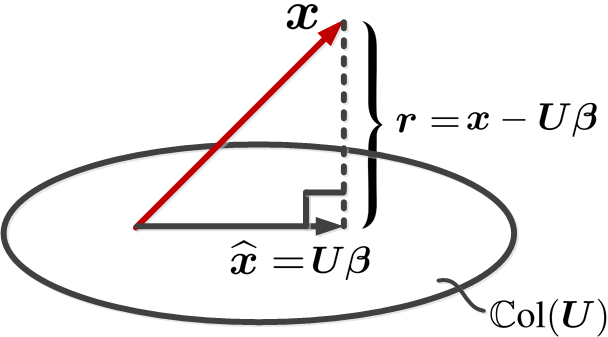
\includegraphics[width=2.2in]{./images/residual_and_space}
\caption{The residual and projection onto the column space of $\boldsymbol{U}$. Credit of image is for \cite{ghojogh2019unsupervised}.}
\label{figure_residual_and_space}
\end{figure}

Plugging Eq. (\ref{equation_beta}) in Eq. (\ref{equation_projection}) gives us:
\begin{align*}
\widehat{\boldsymbol{x}} = \boldsymbol{U} (\boldsymbol{U}^\top \boldsymbol{U})^{-1} \boldsymbol{U}^\top \boldsymbol{x}.
\end{align*}
We define:
\begin{align}\label{equation_hat_matrix}
\mathbb{R}^{d \times d} \ni \boldsymbol{\Pi} := \boldsymbol{U} (\boldsymbol{U}^\top \boldsymbol{U})^{-1} \boldsymbol{U}^\top,
\end{align}
as ``projection matrix'' because it projects $\boldsymbol{x}$ onto $\mathbb{C}\text{ol}(\boldsymbol{U})$ (and reconstructs back).
Note that $\boldsymbol{\Pi}$ is also referred to as the ``hat matrix'' in the literature because it puts a hat on top of $\boldsymbol{x}$.

If the vectors $\{\boldsymbol{u}_1, \dots, \boldsymbol{u}_p\}$ are orthonormal (the matrix $\boldsymbol{U}$ is orthogonal), we have $\boldsymbol{U}^\top = \boldsymbol{U}^{-1}$ and thus $\boldsymbol{U}^\top \boldsymbol{U} = \boldsymbol{I}$. Therefore, Eq. (\ref{equation_hat_matrix}) is simplified:
\begin{align}
& \boldsymbol{\Pi} = \boldsymbol{U} \boldsymbol{U}^\top.
\end{align}
So, we have:
\begin{align}\label{equation_x_hat}
\widehat{\boldsymbol{x}} = \boldsymbol{\Pi}\, \boldsymbol{x} = \boldsymbol{U} \boldsymbol{U}^\top \boldsymbol{x}.
\end{align}

\subsubsection{Projection onto a Subspace}\label{section_projection_subspace}

In subspace learning, the projection of a vector $\boldsymbol{x} \in \mathbb{R}^d$ onto the column space of $\boldsymbol{U} \in \mathbb{R}^{d \times p}$ (a $p$-dimensional subspace spanned by $\{\boldsymbol{u}_j\}_{j=1}^p$ where $\boldsymbol{u}_j \in \mathbb{R}^d$) is defined as:
\begin{align}
&\mathbb{R}^{p} \ni \widetilde{\boldsymbol{x}} := \boldsymbol{U}^\top \boldsymbol{x}, \label{equation_projection_training_onePoint_severalDirections} \\
&\mathbb{R}^{d} \ni \widehat{\boldsymbol{x}} := \boldsymbol{U}\boldsymbol{U}^\top \boldsymbol{x} = \boldsymbol{U} \widetilde{\boldsymbol{x}}, \label{equation_reconstruction_training_onePoint_severalDirections}
\end{align}
where $\widetilde{\boldsymbol{x}}$ and $\widehat{\boldsymbol{x}}$ denote the projection and reconstruction of $\boldsymbol{x}$, respectively.

If we have $n$ data points, $\{\boldsymbol{x}_i\}_{i=1}^n$, which can be stored column-wise in a matrix $\boldsymbol{X} \in \mathbb{R}^{d \times n}$, the projection and reconstruction of $\boldsymbol{X}$ are defined as:
\begin{align}
&\mathbb{R}^{p \times n} \ni \widetilde{\boldsymbol{X}} := \boldsymbol{U}^\top \boldsymbol{X}, \label{equation_projection_training_SeveralPoints_severalDirections} \\
&\mathbb{R}^{d \times n} \ni \widehat{\boldsymbol{X}} := \boldsymbol{U}\boldsymbol{U}^\top \boldsymbol{X} = \boldsymbol{U} \widetilde{\boldsymbol{X}}, \label{equation_reconstruction_training_SeveralPoints_severalDirections}
\end{align}
respectively.

If we have an out-of-sample data point $\boldsymbol{x}_t$ which was not used in calculation of $\boldsymbol{U}$, the projection and reconstruction of it are defined as:
\begin{align}
&\mathbb{R}^{p} \ni \widetilde{\boldsymbol{x}}_t := \boldsymbol{U}^\top \boldsymbol{x}_t, \label{equation_projection_outOfSample_onePoint_severalDirections} \\
&\mathbb{R}^{d} \ni \widehat{\boldsymbol{x}}_t := \boldsymbol{U}\boldsymbol{U}^\top \boldsymbol{x}_t = \boldsymbol{U} \widetilde{\boldsymbol{x}}_t, \label{equation_reconstruction_outOfSample_onePoint_severalDirections}
\end{align}
respectively.

In case we have $n_t$ out-of-sample data points, $\{\boldsymbol{x}_{t,i}\}_{i=1}^{n_t}$, which can be stored column-wise in a matrix $\boldsymbol{X}_t \in \mathbb{R}^{d \times n_t}$, the projection and reconstruction of $\boldsymbol{X}_t$ are defined as:
\begin{align}
&\mathbb{R}^{p \times n_t} \ni \widetilde{\boldsymbol{X}}_t := \boldsymbol{U}^\top \boldsymbol{X}_t, \label{equation_projection_outOfSample_SeveralPoints_severalDirections} \\
&\mathbb{R}^{d \times n_t} \ni \widehat{\boldsymbol{X}}_t := \boldsymbol{U}\boldsymbol{U}^\top \boldsymbol{X}_t = \boldsymbol{U} \widetilde{\boldsymbol{X}}_t, \label{equation_reconstruction_outOfSample_SeveralPoints_severalDirections}
\end{align}
respectively.

For the properties of the projection matrix $\boldsymbol{U}$, refer to \cite{ghojogh2019unsupervised}.

\subsection{Locality Preserving Projection}

LPP assumes that the embeddings of data points are obtained by a linear projection. It approximates Laplacian eigenmap linearly. We want to find the embeddings of data points $\boldsymbol{X} = [\boldsymbol{x}_1, \dots, \boldsymbol{x}_n] \in \mathbb{R}^{d \times n}$ using linear projection. 

\subsubsection{One-dimensional Subspace}

For derivation of LPP optimization, we assume $p=1$ so the projection is onto a line with projection vector $\boldsymbol{u} \in \mathbb{R}^d$. Later, we will extend to higher values for $p$. In this case, the vector of projections of all points is:
\begin{align}\label{equation_LPP_projection_to_line}
\mathbb{R}^{1 \times n} \ni \boldsymbol{Y} = [y_1, y_2, \dots, y_n] := \boldsymbol{u}^\top \boldsymbol{X}.
\end{align}
Hence, the one-dimensional embedding of every point is:
\begin{align}\label{equation_LPP_projection_to_line_2}
\mathbb{R} \ni y_i = \boldsymbol{u}^\top \boldsymbol{x}_i, \quad \forall i \in \{1, \dots, n\}.
\end{align}

% LPP assumes that these embedding vectors are found by linear projection. As we discussed in Section \ref{section_projection_subspace}, projected data $\widetilde{\boldsymbol{X}}$ are stored column-wise. Hence, we have:
% \begin{align}
% &\mathbb{R}^{p} \ni \boldsymbol{y} = \widetilde{\boldsymbol{x}} \overset{(\ref{equation_projection_training_SeveralPoints_severalDirections})}{=} \boldsymbol{x}^\top \boldsymbol{U}, \\
% &\mathbb{R}^{n \times p} \ni \boldsymbol{Y} = \widetilde{\boldsymbol{X}}^\top \overset{(\ref{equation_projection_training_SeveralPoints_severalDirections})}{=} \boldsymbol{X}^\top \boldsymbol{U}.
% \end{align}

Inspired by Eq. (\ref{equation_optimization_Laplacian_eigenmap_1}) for Laplacian eigenmap, the optimization for obtaining the one-dimensional embedding is:
\begin{align}\label{equation_optimization_LPP_1}
\underset{\boldsymbol{Y}}{\text{minimize}} \quad \sum_{i=1}^n \sum_{j=1}^n w_{ij}\, (y_i - y_j)^2,
\end{align}
for the same interpretation that we had in Laplacian eigenmap. 

\begin{proposition}[\cite{he2004locality}]\label{proposition_LPP_y_L_y}
We have:
\begin{align}
\frac{1}{2} \sum_{i=1}^n \sum_{j=1}^n w_{ij} (y_i - y_j)^2 = \boldsymbol{u}^\top \boldsymbol{X} \boldsymbol{L} \boldsymbol{X}^\top \boldsymbol{u}.
\end{align}
\end{proposition}
\begin{proof}
The proof is very similar to the proof of Proposition \ref{proposition_spectral_clustering_f_L_f}. We have:
\begin{align*}
&\boldsymbol{u}^\top \boldsymbol{X} \boldsymbol{L} \boldsymbol{X}^\top \boldsymbol{u} \overset{(\ref{equation_Laplacian_matrix})}{=} \boldsymbol{u}^\top \boldsymbol{X} (\boldsymbol{D} - \boldsymbol{W}) \boldsymbol{X}^\top \boldsymbol{u} \\
&= \boldsymbol{u}^\top \boldsymbol{X} \boldsymbol{D} \boldsymbol{X}^\top \boldsymbol{u} - \boldsymbol{u}^\top \boldsymbol{X} \boldsymbol{W} \boldsymbol{X}^\top \boldsymbol{u} \\
&\overset{(a)}{=} \sum_{i=1}^n \boldsymbol{u}^\top \boldsymbol{x}_i\, d_i\, \boldsymbol{x}_i^\top \boldsymbol{u} - \sum_{i=1}^n \sum_{j=1}^n \boldsymbol{u}^\top \boldsymbol{x}_i\, w_{ij}\, \boldsymbol{x}_j^\top \boldsymbol{u} \\
&= \frac{1}{2} \Big(2\sum_{i=1}^n \boldsymbol{u}^\top \boldsymbol{x}_i\, d_i\, \boldsymbol{x}_i^\top \boldsymbol{u} - 2\sum_{i=1}^n \sum_{j=1}^n \boldsymbol{u}^\top \boldsymbol{x}_i\, w_{ij}\, \boldsymbol{x}_j^\top \boldsymbol{u}\Big) \\
&\overset{(b)}{=} \frac{1}{2} \Big(2\sum_{i=1}^n (\boldsymbol{u}^\top \boldsymbol{x}_i)^2 d_i - 2\sum_{i=1}^n \sum_{j=1}^n (\boldsymbol{u}^\top \boldsymbol{x}_i) (\boldsymbol{u}^\top \boldsymbol{x}_j) w_{ij}\Big) \\
&\overset{(c)}{=} \frac{1}{2} \Big(\sum_{i=1}^n (\boldsymbol{u}^\top \boldsymbol{x}_i)^2 d_i + \sum_{j=1}^n (\boldsymbol{u}^\top \boldsymbol{x}_j)^2 d_j \\
&~~~~~~~~~~~~~~~~~~~~~~~~~~~ - 2\sum_{i=1}^n \sum_{j=1}^n (\boldsymbol{u}^\top \boldsymbol{x}_i) (\boldsymbol{u}^\top \boldsymbol{x}_j) w_{ij}\Big) 
\end{align*}
\begin{align*}
&\overset{(\ref{equation_degree_matrix})}{=} \frac{1}{2} \Big(\sum_{i=1}^n (\boldsymbol{u}^\top \boldsymbol{x}_i)^2 \sum_{j=1}^n w_{ij} + \sum_{j=1}^n (\boldsymbol{u}^\top \boldsymbol{x}_j)^2 \sum_{i=1}^n w_{ji} \\
&~~~~~~~~~~~~~~~~~~~~~~~~~~~ - 2\sum_{i=1}^n \sum_{j=1}^n (\boldsymbol{u}^\top \boldsymbol{x}_i) (\boldsymbol{u}^\top \boldsymbol{x}_j) w_{ij} \Big) \\
&\overset{(d)}{=} \frac{1}{2} \Big(\sum_{i=1}^n (\boldsymbol{u}^\top \boldsymbol{x}_i)^2 \sum_{j=1}^n w_{ij} + \sum_{j=1}^n (\boldsymbol{u}^\top \boldsymbol{x}_j)^2 \sum_{i=1}^n w_{ij} \\
&~~~~~~~~~~~~~~~~~~~~~~~~~~~ - 2\sum_{i=1}^n \sum_{j=1}^n (\boldsymbol{u}^\top \boldsymbol{x}_i) (\boldsymbol{u}^\top \boldsymbol{x}_j) w_{ij} \Big) \\
&= \frac{1}{2} \sum_{i=1}^n \sum_{j=1}^n w_{ij} (\boldsymbol{u}^\top \boldsymbol{x}_i - \boldsymbol{u}^\top \boldsymbol{x}_j)^2 \\
&\overset{(\ref{equation_LPP_projection_to_line_2})}{=} \frac{1}{2} \sum_{i=1}^n \sum_{j=1}^n w_{ij} (y_i - y_j)^2,
\end{align*}
where $(a)$ notices that $\boldsymbol{D}$ is a diagonal matrix, $(b)$ is because $\boldsymbol{u}^\top \boldsymbol{x}_i = \boldsymbol{x}_i^\top \boldsymbol{u}_i \in \mathbb{R}$, $(c)$ is because we can replace the dummy index $i$ with $j$, and $(d)$ notices that $w_{ij} = w_{ji}$ as we usually use symmetric similarity measures. Q.E.D.
\end{proof}

According to Proposition \ref{proposition_LPP_y_L_y}, we restate Eq. (\ref{equation_optimization_LPP_1}) with adding a constraint inspired by Eq. (\ref{equation_optimization_Laplacian_eigenmap_3}) as:
\begin{equation}\label{equation_optimization_LPP_2}
\begin{aligned}
& \underset{\boldsymbol{u}}{\text{minimize}}
& & \boldsymbol{u}^\top \boldsymbol{X} \boldsymbol{L} \boldsymbol{X}^\top \boldsymbol{u} \\
& \text{subject to}
& & 
\boldsymbol{u}^\top \boldsymbol{X} \boldsymbol{D} \boldsymbol{X}^\top \boldsymbol{u} = 1,
\end{aligned}
\end{equation}
where $\boldsymbol{L}$ and $\boldsymbol{D}$ are the Laplacian and degree matrix of the adjacency matrix, respectively. Note that the objective variable has been changed to the projection vector $\boldsymbol{u}$.

The Lagrangian for this optimization problem is \cite{boyd2004convex}:
\begin{align*}
\mathcal{L} = \boldsymbol{u}^\top \boldsymbol{X} \boldsymbol{L} \boldsymbol{X}^\top \boldsymbol{u} - \lambda^\top (\boldsymbol{u}^\top \boldsymbol{X} \boldsymbol{D} \boldsymbol{X}^\top \boldsymbol{u} - 1),
\end{align*}
where $\lambda$ is the dual variable. Setting the derivative of Lagrangian to zero gives:
\begin{align}
&\mathbb{R}^{d} \ni \frac{\partial \mathcal{L}}{\partial \boldsymbol{u}} = 2 \boldsymbol{X} \boldsymbol{L} \boldsymbol{X}^\top \boldsymbol{u} - 2 \lambda \boldsymbol{X} \boldsymbol{D} \boldsymbol{X}^\top \boldsymbol{u} \overset{\text{set}}{=} \boldsymbol{0} \nonumber \\
&~~~~~~~~~~~ \implies \boldsymbol{X} \boldsymbol{L} \boldsymbol{X}^\top \boldsymbol{u} = \lambda \boldsymbol{X} \boldsymbol{D} \boldsymbol{X}^\top \boldsymbol{u},
\end{align}
which is the generalized eigenvalue problem $(\boldsymbol{X} \boldsymbol{L} \boldsymbol{X}^\top, \boldsymbol{X} \boldsymbol{D} \boldsymbol{X}^\top)$ where $\boldsymbol{u}$ is the eigenvector \cite{ghojogh2019eigenvalue}. The embedded points are obtained using Eq. (\ref{equation_LPP_projection_to_line}).

\subsubsection{Multi-dimensional Subspace}

Now, we extend LPP to linear projection onto a span of $p$ basis vectors. In other words, we extend it to have $p$-dimensional subspace.
The embedding of $\boldsymbol{x}_i$ is denoted by $\boldsymbol{y}_i \in \mathbb{R}^p$. In LPP, we put the embedding vectors column-wise in matrix $\boldsymbol{Y} = [\boldsymbol{y}_1, \boldsymbol{y}_2, \dots, \boldsymbol{y}_n] \in \mathbb{R}^{p \times n}$.
In this case, the projection is:
\begin{align}\label{equation_LPP_projection_to_subspace}
\mathbb{R}^{p \times n} \ni \boldsymbol{Y} := \boldsymbol{U}^\top \boldsymbol{X},
\end{align}
where $\boldsymbol{U} = [\boldsymbol{u}_1, \dots, \boldsymbol{u}_p] \in \mathbb{R}^{d \times p}$ is the projection matrix onto its column space. 

The Eq. (\ref{equation_optimization_Laplacian_eigenmap_2}) can be extended to multi-dimensional subspace as:
\begin{equation}\label{equation_optimization_Laplacian_eigenmap_2_multi}
\begin{aligned}
& \underset{\boldsymbol{U}}{\text{minimize}}
& & \textbf{tr}(\boldsymbol{U}^\top \boldsymbol{X} \boldsymbol{L} \boldsymbol{X}^\top \boldsymbol{U}) \\
& \text{subject to}
& & 
\boldsymbol{U}^\top \boldsymbol{X} \boldsymbol{D} \boldsymbol{X}^\top \boldsymbol{U} = \boldsymbol{I}.
\end{aligned}
\end{equation}
In optimization, it is assumed that the dimensionality of $\boldsymbol{U}$ is $d \times d$ but we will truncate it to $d \times p$ after solving the optimization. 

The Lagrangian for this optimization problem is \cite{boyd2004convex}:
\begin{align*}
\mathcal{L} = \textbf{tr}(\boldsymbol{U}^\top \boldsymbol{X} \boldsymbol{L} \boldsymbol{X}^\top \boldsymbol{U}) - \textbf{tr}(\boldsymbol{\Lambda}^\top (\boldsymbol{U}^\top \boldsymbol{X} \boldsymbol{D} \boldsymbol{X}^\top \boldsymbol{U} - \boldsymbol{I})),
\end{align*}
where $\boldsymbol{\Lambda}$ is the diagonal matrix with the dual variables. Setting the derivative of Lagrangian to zero gives:
\begin{align}
&\mathbb{R}^{d \times d} \ni \frac{\partial \mathcal{L}}{\partial \boldsymbol{D}} = 2 \boldsymbol{X} \boldsymbol{L} \boldsymbol{X}^\top \boldsymbol{U} - 2 \boldsymbol{X} \boldsymbol{D} \boldsymbol{X}^\top \boldsymbol{U} \boldsymbol{\Lambda} \overset{\text{set}}{=} \boldsymbol{0} \nonumber \\
&~~~~~~~~~~~ \implies \boldsymbol{X} \boldsymbol{L} \boldsymbol{X}^\top \boldsymbol{U} = \boldsymbol{X} \boldsymbol{D} \boldsymbol{X}^\top \boldsymbol{U} \boldsymbol{\Lambda}, \label{equation_LPP_multi_solution}
\end{align}
which is the generalized eigenvalue problem $(\boldsymbol{X} \boldsymbol{L} \boldsymbol{X}^\top, \boldsymbol{X} \boldsymbol{D} \boldsymbol{X}^\top)$ where columns of $\boldsymbol{U}$ are the eigenvectors \cite{ghojogh2019eigenvalue}. 
As it is a minimization problem, the columns of $\boldsymbol{U}$, which are the eigenvectors, are sorted from the corresponding smallest to largest eigenvalues. Moreover, as we have Laplacian matrix, we have one eigenvector with eigenvalue zero which should be ignored (see Section \ref{section_eig_Laplacian}). 
The embedded points are obtained using Eq. (\ref{equation_LPP_projection_to_subspace}).

\subsection{Kernel Locality Preserving Projection}

Kernel LPP, also called kernel supervised LPP,  \cite{cheng2005supervised,li2008kernel} performs LPP in the feature space. 
Assume $\boldsymbol{\phi}(.)$ denotes the pulling function to the feature space. 
According to representation theory \cite{alperin1993local}, any pulled solution (direction) $\boldsymbol{\phi}(\boldsymbol{u}) \in \mathcal{H}$ must lie in the span of all the training vectors pulled to $\mathcal{H}$, i.e., $\boldsymbol{\Phi}(\boldsymbol{X}) = [\boldsymbol{\phi}(\boldsymbol{x}_1), \dots, \boldsymbol{\phi}(\boldsymbol{x}_n)] \in \mathbb{R}^{t\times n}$. 
Hence, $\mathbb{R}^{t} \ni \boldsymbol{\phi}(\boldsymbol{u}) = \sum_{i=1}^n \theta_i\, \boldsymbol{\phi}(\boldsymbol{x}_i) = \boldsymbol{\Phi}(\boldsymbol{X})\, \boldsymbol{\theta}$ where $\mathbb{R}^n \ni \boldsymbol{\theta} = [\theta_1, \dots, \theta_n]^\top$ is the unknown vector of coefficients.
Considering multiple projection directions, we have:
\begin{align}\label{equation_Phi_U}
\mathbb{R}^{t \times p} \ni \boldsymbol{\Phi}(\boldsymbol{U}) = \boldsymbol{\Phi}(\boldsymbol{X})\, \boldsymbol{\Theta},
\end{align}
where $\mathbb{R}^{n \times p} \ni \boldsymbol{\Theta} = [\boldsymbol{\theta}_1, \dots, \boldsymbol{\theta}_p]$.
Therefore, the objective function in Eq. (\ref{equation_optimization_Laplacian_eigenmap_2_multi}) is converted to:
\begin{align*}
& \textbf{tr}(\boldsymbol{\Phi}(\boldsymbol{U})^\top \boldsymbol{\Phi}(\boldsymbol{X}) \boldsymbol{L} \boldsymbol{\Phi}(\boldsymbol{X})^\top \boldsymbol{\Phi}(\boldsymbol{U})) \\
& \overset{(\ref{equation_Phi_U})}{=} \textbf{tr}(\boldsymbol{\Theta}^\top \boldsymbol{\Phi}(\boldsymbol{X})^\top \boldsymbol{\Phi}(\boldsymbol{X}) \boldsymbol{L} \boldsymbol{\Phi}(\boldsymbol{X})^\top \boldsymbol{\Phi}(\boldsymbol{X})\, \boldsymbol{\Theta}) \\
&= \textbf{tr}(\boldsymbol{\Theta}^\top \boldsymbol{K}_x \boldsymbol{L} \boldsymbol{K}_x\, \boldsymbol{\Theta}),
\end{align*}
where:
\begin{align}\label{equation_kernel_of_data}
\mathbb{R}^{n \times n} \ni \boldsymbol{K}_x := \boldsymbol{\Phi}(\boldsymbol{X})^\top \boldsymbol{\Phi}(\boldsymbol{X}),
\end{align}
is the kernel of data \cite{hofmann2008kernel}. 

Similarly, the constraint of Eq. (\ref{equation_optimization_Laplacian_eigenmap_2_multi}) is converted to $\boldsymbol{\Theta}^\top \boldsymbol{K}_x \boldsymbol{D} \boldsymbol{K}_x\, \boldsymbol{\Theta}$.

Finally, the Eq. (\ref{equation_optimization_Laplacian_eigenmap_2_multi}) is changed to:

\begin{equation}\label{equation_optimization_LPP_kernel}
\begin{aligned}
& \underset{\boldsymbol{\Theta}}{\text{minimize}}
& & \textbf{tr}(\boldsymbol{\Theta}^\top \boldsymbol{K}_x \boldsymbol{L} \boldsymbol{K}_x\, \boldsymbol{\Theta}) \\
& \text{subject to}
& & 
\boldsymbol{\Theta}^\top \boldsymbol{K}_x \boldsymbol{D} \boldsymbol{K}_x\, \boldsymbol{\Theta} = \boldsymbol{I},
\end{aligned}
\end{equation}

where $\boldsymbol{\Theta}$ is the optimization variable. 
The solution to this problem is similar to the solution of Eq. (\ref{equation_optimization_Laplacian_eigenmap_2_multi}). So, its solution is the generalized eigenvalue problem $(\boldsymbol{K}_x \boldsymbol{L} \boldsymbol{K}_x^\top, \boldsymbol{K}_x \boldsymbol{D} \boldsymbol{K}_x^\top)$ where columns of $\boldsymbol{\Theta}$ are the eigenvectors \cite{ghojogh2019eigenvalue}. 
Sorting the matrix $\boldsymbol{\Theta}$ and ignoring the eigenvector with zero eigenvalue (see Section \ref{section_eig_Laplacian}) is done as explained before. The $p$ smallest eigenvectors form $\boldsymbol{\Theta} \in \mathbb{R}^{n \times p}$. 
The embedded data are obtained as:
\begin{align}
\mathbb{R}^{p \times n} \ni \boldsymbol{Y} &\overset{(\ref{equation_LPP_projection_to_subspace})}{=} \boldsymbol{\Phi}(\boldsymbol{U})^\top \boldsymbol{\Phi}(\boldsymbol{X}) \overset{(\ref{equation_Phi_U})}{=} \boldsymbol{\Theta}^\top \boldsymbol{\Phi}(\boldsymbol{X})^\top \boldsymbol{\Phi}(\boldsymbol{X}) \nonumber \\
&\overset{(\ref{equation_kernel_of_data})}{=} \boldsymbol{\Theta}^\top \boldsymbol{K}_x. \label{equation_kernel_LPP_embedding}
\end{align}


\subsection{Other Improvements over Locality Preserving Projection}

There have been many improvements over the basic LPP. Some examples of these developments are supervised LPP \cite{wong2012supervised}, extended LPP \cite{shikkenawis2012improving}, multiview uncorrelated LPP \cite{yin2019multiview}, graph-optimized LPP \cite{zhang2010graph}, and LPP for Grassmann manifold \cite{wang2017locality}. 
For image recognition purposes, a two-dimensional (2D) LPP, \cite{chen20072d} is proposed whose robust version is \cite{chen20192drlpp} and some of its applications are \cite{hu2007two,xu2009one}.
A survey on LPP variants can be found in \cite{shikkenawis2016some}. 
LPP has been shown to be effective for different applications such as document clustering \cite{cai2005document}, face recognition \cite{he2003learning,yu2006face,yang2017discriminant}, and speech recognition \cite{tang2008study}. 


\section{Graph Embedding}\label{section_graph_embedding}

Graph Embedding (GE) \cite{yan2005graph,yan2006graph} is a generalized dimensionality reduction method where the graph of data is embedded in the lower dimensional space \cite{chang2014graph}. 
Note that graph embedding is referred to as two different families of methods in the literature. In the first sense, including GE \cite{yan2005graph,yan2006graph}, it refers to embedding the graph of data in the lower dimensional space. The second sense, however, refers to embedding every node of data graph in a subspace \cite{goyal2018graph}. Here, our focus is on embedding the whole data graph. 
Note that there exist some other generalized subspace learning methods, such as Roweis discriminant analysis \cite{ghojogh2020generalized}, in the literature.

\subsection{Direct Graph Embedding}

Consider the high dimensional data points $\{\boldsymbol{x}_i \in \mathbb{R}^d\}_{i=1}^n$. We want to reduce the dimensionality of data from $d$ to $p \leq d$ to have $\{\boldsymbol{y}_i \in \mathbb{R}^p\}_{i=1}^n$, where usually $p \ll d$.
We denote $\boldsymbol{X} := [\boldsymbol{x}_1, \dots, \boldsymbol{x}_n] \in \mathbb{R}^{d \times n}$ and $\boldsymbol{Y} := [\boldsymbol{y}_1, \dots, \boldsymbol{y}_n] \in \mathbb{R}^{p \times n}$.
Similar to spectral clustering, we create an adjacency matrix using Eq. (\ref{equation_adjacency_matrix}). The elements $w_{ij}$ can be determined by the RBF kernel, i.e. Eq. (\ref{equation_RBF_kernel}), or the simple-minded approach, i.e. Eq. (\ref{equation_simple_minded}).

The objective function of optimization in direct GE \cite{yan2005graph,yan2006graph} is inspired by Eq. (\ref{equation_minimization_spectral_clustering_w_f}) or Eq. (\ref{equation_spectral_clustering_optimization_multiple_2}) in spectral clustering:
\begin{equation}\label{equation_optimization_direct_graph_embedding}
\begin{aligned}
& \underset{\boldsymbol{Y}}{\text{minimize}}
& & \sum_{i=1}^n \sum_{j=1}^n w_{ij}\, \|\boldsymbol{y}_i - \boldsymbol{y}_j\|_2^2 \\
& \text{subject to}
& & 
\boldsymbol{Y}^\top \boldsymbol{B} \boldsymbol{Y} = \boldsymbol{I},
\end{aligned}
\end{equation}
where $\boldsymbol{B} \succeq 0$ is called the constraint matrix. 
According to Proposition \ref{proposition_spectral_clustering_f_L_f}, this optimization problem is equivalent to:
\begin{equation}\label{equation_optimization_direct_graph_embedding_2}
\begin{aligned}
& \underset{\boldsymbol{Y}}{\text{minimize}}
& & \boldsymbol{Y}^\top \boldsymbol{L} \boldsymbol{Y} \\
& \text{subject to}
& & 
\boldsymbol{Y}^\top \boldsymbol{B} \boldsymbol{Y} = \boldsymbol{I},
\end{aligned}
\end{equation}
where $\boldsymbol{L}$ is the Laplacian of graph of data. 

The Lagrangian for this optimization problem is \cite{boyd2004convex}:
\begin{align*}
\mathcal{L} = \boldsymbol{Y}^\top \boldsymbol{L} \boldsymbol{Y} - \textbf{tr}(\boldsymbol{\Lambda}^\top (\boldsymbol{Y}^\top \boldsymbol{B} \boldsymbol{Y} - \boldsymbol{I})),
\end{align*}
where $\boldsymbol{\Lambda}$ is the diagonal matrix with the dual variables. Setting the derivative of Lagrangian to zero gives:
\begin{align}
&\mathbb{R}^{n \times n} \ni \frac{\partial \mathcal{L}}{\partial \boldsymbol{Y}} = 2 \boldsymbol{L} \boldsymbol{Y} - 2 \boldsymbol{B} \boldsymbol{Y} \boldsymbol{\Lambda} \overset{\text{set}}{=} \boldsymbol{0} \nonumber \\
&~~~~~~~~~~~ \implies \boldsymbol{L} \boldsymbol{Y} = \boldsymbol{B} \boldsymbol{Y} \boldsymbol{\Lambda},
\end{align}
which is the generalized eigenvalue problem $(\boldsymbol{L}, \boldsymbol{B})$ where columns of $\boldsymbol{Y}$ are the eigenvectors \cite{ghojogh2019eigenvalue}. 
Sorting the matrix $\boldsymbol{Y}$ and ignoring the eigenvector with zero eigenvalue (see Section \ref{section_eig_Laplacian}) is done as explained before. 

\subsection{Linearized Graph Embedding}

As we had for LPP, linearized GE \cite{yan2005graph,yan2006graph} assumes that the embedded data can be obtained by a linear projection onto the column space of a projection matrix $\boldsymbol{U} \in \mathbb{R}^{d \times p}$. Hence, linearized GE uses similar optimization to Eq. (\ref{equation_optimization_Laplacian_eigenmap_2_multi}):
\begin{equation}\label{equation_optimization_linearized_graph_embedding}
\begin{aligned}
& \underset{\boldsymbol{U}}{\text{minimize}}
& & \textbf{tr}(\boldsymbol{U}^\top \boldsymbol{X} \boldsymbol{L} \boldsymbol{X}^\top \boldsymbol{U}) \\
& \text{subject to}
& & 
\boldsymbol{U}^\top \boldsymbol{X} \boldsymbol{B} \boldsymbol{X}^\top \boldsymbol{U} = \boldsymbol{I},
\end{aligned}
\end{equation}
whose solution is the generalized eigenvalue problem $(\boldsymbol{X} \boldsymbol{L} \boldsymbol{X}^\top, \boldsymbol{X} \boldsymbol{B} \boldsymbol{X}^\top)$, similar to Eq. (\ref{equation_LPP_multi_solution}).

Another approach for linearized GE is a slight revision to Eq. (\ref{equation_optimization_linearized_graph_embedding}) which is \cite{yan2005graph}:
\begin{equation}\label{equation_optimization_linearized_graph_embedding2}
\begin{aligned}
& \underset{\boldsymbol{U}}{\text{minimize}}
& & \textbf{tr}(\boldsymbol{U}^\top \boldsymbol{X} \boldsymbol{L} \boldsymbol{X}^\top \boldsymbol{U}) \\
& \text{subject to}
& & 
\boldsymbol{U}^\top \boldsymbol{U} = \boldsymbol{I},
\end{aligned}
\end{equation}
whose solution is the eigenvalue decomposition of $\boldsymbol{X} \boldsymbol{L} \boldsymbol{X}^\top$. 

\subsection{Kernelized Graph Embedding}

Kernelized GE \cite{yan2005graph,yan2006graph} performs the linearized GE in the feature space. It uses a similar optimization problem as Eq. (\ref{equation_optimization_LPP_kernel}):
\begin{equation}\label{equation_optimization_kernelized_GE}
\begin{aligned}
& \underset{\boldsymbol{\Theta}}{\text{minimize}}
& & \textbf{tr}(\boldsymbol{\Theta}^\top \boldsymbol{K}_x \boldsymbol{L} \boldsymbol{K}_x\, \boldsymbol{\Theta}) \\
& \text{subject to}
& & 
\boldsymbol{\Theta}^\top \boldsymbol{K}_x \boldsymbol{B} \boldsymbol{K}_x\, \boldsymbol{\Theta} = \boldsymbol{I},
\end{aligned}
\end{equation}
whose solution is the generalized eigenvalue problem $(\boldsymbol{K}_x \boldsymbol{L} \boldsymbol{K}_x^\top, \boldsymbol{K}_x \boldsymbol{B} \boldsymbol{K}_x^\top)$ where columns of $\boldsymbol{\Theta}$ are the eigenvectors \cite{ghojogh2019eigenvalue}.
Sorting the matrix $\boldsymbol{\Theta}$ and ignoring the eigenvector with zero eigenvalue (see Section \ref{section_eig_Laplacian}) is done as explained before. The embedding is then obtained using Eq. (\ref{equation_kernel_LPP_embedding}). 

Another approach for linearized GE is a slight revision to Eq. (\ref{equation_optimization_kernelized_GE}). 
This approach is the kernelized version of Eq. (\ref{equation_optimization_linearized_graph_embedding2}) and is \cite{yan2005graph}:
\begin{equation}\label{equation_optimization_kernelized_GE_2}
\begin{aligned}
& \underset{\boldsymbol{\Theta}}{\text{minimize}}
& & \textbf{tr}(\boldsymbol{\Theta}^\top \boldsymbol{K}_x \boldsymbol{L} \boldsymbol{K}_x\, \boldsymbol{\Theta}) \\
& \text{subject to}
& & 
\boldsymbol{\Theta}^\top \boldsymbol{K}_x \boldsymbol{\Theta} = \boldsymbol{I},
\end{aligned}
\end{equation}
whose solution is the generalized eigenvalue problem $(\boldsymbol{K}_x \boldsymbol{L} \boldsymbol{K}_x^\top, \boldsymbol{K}_x)$.

\subsection{Special Cases of Graph Embedding}

GE is a generalized subspace learning method whose special cases are some of the well-known dimensionality reduction methods. These special cases are cases of either direct, or linearized, or kernelized GE. Some of the special cases are Laplacian eigenmap, LPP, kernel LPP, Principal Component Analysis (PCA), kernel PCA, Fisher Discriminant Analysis (FDA), kernel FDA, Multidimensional Scaling (MDS), Isomap, and Locally Linear Embedding (LLE). 

\subsubsection{Laplacian Eigenmap}

Comparing Eq. (\ref{equation_optimization_Laplacian_eigenmap_2}) of Laplacian eigenmap with Eq. (\ref{equation_optimization_direct_graph_embedding_2}), we see that $\boldsymbol{B} = \boldsymbol{I}$. Also comparing Eq. (\ref{equation_optimization_Laplacian_eigenmap_3}) as the second approach of Laplacian eigenmap, with Eq. (\ref{equation_optimization_direct_graph_embedding_2}) shows that $\boldsymbol{B} = \boldsymbol{D}$. Hence, Laplacian eigenmap is a special case of direct GE.

\subsubsection{LPP and Kernel LPP}

Comparing Eq. (\ref{equation_optimization_Laplacian_eigenmap_2_multi}) with Eq. (\ref{equation_optimization_linearized_graph_embedding}) and also comparing Eq. (\ref{equation_optimization_LPP_kernel}) with Eq. (\ref{equation_optimization_kernelized_GE}) show that LPP and kernel LPP are special cases of linearized GE and kernelized GE, respectively. 

\subsubsection{PCA and Kernel PCA}

The optimization of PCA is \cite{ghojogh2019unsupervised}:
\begin{equation}\label{equation_PCA}
\begin{aligned}
& \underset{\boldsymbol{U}}{\text{minimize}}
& & \textbf{tr}(\boldsymbol{U}^\top \boldsymbol{S} \boldsymbol{U}) \overset{(a)}{=} \textbf{tr}(\boldsymbol{U}^\top \boldsymbol{X} \boldsymbol{X}^\top \boldsymbol{U}) \\
& \text{subject to}
& & 
\boldsymbol{U}^\top \boldsymbol{U} = \boldsymbol{I},
\end{aligned}
\end{equation}
where $\boldsymbol{U}$ is the projection matrix, $\boldsymbol{S}$ is the covariance matrix of data, and $(a)$ is because of $\boldsymbol{S} = \boldsymbol{X} \boldsymbol{X}^\top$ assuming that data $\boldsymbol{X}$ are already centered. 
Moreover, the solution of kernel PCA is the eigenvalue decomposition of kernel of data \cite{ghojogh2019unsupervised}; hence, optimization of kernel PCA is the kernelized version of Eq. (\ref{equation_PCA}). 
Comparing Eq. (\ref{equation_PCA}) with Eq. (\ref{equation_optimization_linearized_graph_embedding2}) shows that PCA is a special case of linearized GE with $\boldsymbol{L}=\boldsymbol{I}$. Moreover, kernel PCA is a special case of kernelized GE with $\boldsymbol{L} = \boldsymbol{I}$. 

\subsubsection{FDA and Kernel FDA}

The optimization of FDA is \cite{ghojogh2019fisher,fisher1936use}:
\begin{equation}\label{equation_optimization_FDA_with_S_B}
\begin{aligned}
& \underset{\boldsymbol{U}}{\text{maximize}}
& & \textbf{tr}(\boldsymbol{U}^\top \boldsymbol{S}_B\, \boldsymbol{U}) \\
& \text{subject to}
& & \boldsymbol{U}^\top \boldsymbol{S}_W\, \boldsymbol{U} = \boldsymbol{I},
\end{aligned}
\end{equation}
where $\boldsymbol{S}_B$ and $\boldsymbol{S}_W$ are the between- and within-class scatters, respectively. 
We also have \cite{ye2007least}: 
\begin{align}\label{equation_S_T_as_sum_of_scatters}
\boldsymbol{S} = \boldsymbol{S}_B + \boldsymbol{S}_W \implies \boldsymbol{S}_B = \boldsymbol{S} - \boldsymbol{S}_W,
\end{align}
where $\boldsymbol{S}$ denotes the total covariance of data. Hence, the Fisher criterion, to be maximized, can be restated as:
\begin{align}\label{equation_Fisher_criterion}
& \frac{\textbf{tr}(\boldsymbol{U}^\top \boldsymbol{S}_B\, \boldsymbol{U})}{\textbf{tr}(\boldsymbol{U}^\top \boldsymbol{S}_W\, \boldsymbol{U})} = \frac{\textbf{tr}(\boldsymbol{U}^\top \boldsymbol{S}\, \boldsymbol{U})}{\textbf{tr}(\boldsymbol{U}^\top \boldsymbol{S}_W\, \boldsymbol{U})} - 1,
\end{align}
whose second constant term can be ignored in maximization. Therefore, Eq. (\ref{equation_optimization_FDA_with_S_B}) is restated to \cite{yan2005graph,ghojogh2020generalized}:
\begin{equation}\label{equation_optimization_FDA_with_S_T}
\begin{aligned}
& \underset{\boldsymbol{U}}{\text{maximize}}
& & \textbf{tr}(\boldsymbol{U}^\top \boldsymbol{S}\, \boldsymbol{U}) \overset{(a)}{=} \textbf{tr}(\boldsymbol{U}^\top \boldsymbol{X} \boldsymbol{X}^\top \boldsymbol{U}) \\
& \text{subject to}
& & \boldsymbol{U}^\top \boldsymbol{S}_W\, \boldsymbol{U} = \boldsymbol{I},
\end{aligned}
\end{equation}
where $(a)$ is because of $\boldsymbol{S} = \boldsymbol{X} \boldsymbol{X}^\top$ assuming that data $\boldsymbol{X}$ are already centered. 

Let $c_i$ denote the class to which the point $\boldsymbol{x}_i$ belongs and $\boldsymbol{\mu}_{c_i}$ be the mean of class $c_i$. Let $c$ denote the number of classes and $n_j$ be the sample size of class $j$. For every class $j$, we define $\boldsymbol{e}_j = [e_{j1}, \dots, e_{jn}]^\top \in \mathbb{R}^n$ as:
\begin{align}
e_{ji} = 
\left\{
    \begin{array}{ll}
        1 & \mbox{if } c_i = j, \\
        0 & \mbox{otherwise}.
    \end{array}
\right.
\end{align}
Note that the within scatter can be obtained as \cite{yan2005graph}:
\begin{align}\label{equation_within_scatter_restate_for_GE}
\boldsymbol{S}_W &= \sum_{i=1}^n (\boldsymbol{x}_i - \boldsymbol{\mu}_{c_i}) (\boldsymbol{x}_i - \boldsymbol{\mu}_{c_i})^\top \nonumber \\
&= \boldsymbol{X} (\boldsymbol{I} - \sum_{j=1}^{c} \frac{1}{n_j} \boldsymbol{e}_j \boldsymbol{e}_j^\top) \boldsymbol{X}^\top.
\end{align}
Comparing Eq. (\ref{equation_optimization_FDA_with_S_T}) with Eq. (\ref{equation_optimization_linearized_graph_embedding}) and noticing Eq. (\ref{equation_within_scatter_restate_for_GE}) show that FDA is a special case of linearized GE with $\boldsymbol{L} = \boldsymbol{I}$ and $\boldsymbol{B} = \boldsymbol{I} - \sum_{j=1}^{c} (1/n_j) \boldsymbol{e}_j \boldsymbol{e}_j^\top$. 
Kernel FDA \cite{ghojogh2019fisher,mika1999fisher} is the kernelized version of Eq. (\ref{equation_optimization_FDA_with_S_T}) so it is a special case of kernelized GE with the mentioned $\boldsymbol{L}$ and $\boldsymbol{B}$ matrices. 

\subsubsection{MDS and Isomap}

Kernel classical MDS uses a kernel as \cite{ghojogh2020multidimensional}:
\begin{align}\label{equation_Isomap_kernel}
\mathbb{R}^{n \times n} \ni \boldsymbol{K} = -\frac{1}{2} \boldsymbol{H} \boldsymbol{D} \boldsymbol{H},
\end{align}
where $\boldsymbol{D} \in \mathbb{R}^{n \times n}$ is a matrix with squared Euclidean distance between points and $\mathbb{R}^{n \times n} \ni \boldsymbol{H} := \boldsymbol{I} - (1/n) \boldsymbol{1} \boldsymbol{1}^\top$ is the centering matrix. 
Isomap also applies multidimensional scaling with a geodesic kernel which uses piece-wise Euclidean distance for computing $\boldsymbol{D}$ \cite{tenenbaum2000global,ghojogh2020multidimensional}.
The row summation of this kernel matrix is \cite{yan2005graph,yan2006graph}: 
\begin{align*}
&\sum_{j=1}^n \boldsymbol{K}_{ij} \overset{(\ref{equation_Isomap_kernel})}{=} \sum_{j=1}^n (-\frac{1}{2} \boldsymbol{H} \boldsymbol{D} \boldsymbol{H})_{ij} \\
&= \sum_{j=1}^n \big(-\frac{1}{2} (\boldsymbol{I} - \frac{1}{n} \boldsymbol{1} \boldsymbol{1}^\top) \boldsymbol{D} (\boldsymbol{I} - \frac{1}{n} \boldsymbol{1} \boldsymbol{1}^\top)\big)_{ij} \\
&= \frac{1}{2} \sum_{j=1}^n \big( -\boldsymbol{D}_{ij} + \frac{1}{n} \sum_{i'=1}^n \boldsymbol{D}_{i' j} \\
&~~~~~~~~~~~~~~~~~~~~~~~~~~~~~~ + \frac{1}{n} \sum_{j'=1}^n (\boldsymbol{D}_{i j'} - \frac{1}{n} \sum_{k'=1}^n \boldsymbol{D}_{k' j'}) \big) \\
&= (-\frac{1}{2} \sum_{j=1}^n \boldsymbol{D}_{ij} + \frac{1}{2n} \sum_{j=1}^n \sum_{i'=1}^n \boldsymbol{D}_{i' j}) + (\frac{1}{2n} \sum_{j=1}^n \sum_{j'=1}^n \boldsymbol{D}_{i j'} \\
&~~~~~~ - \frac{1}{2n^2} \sum_{j=1}^n \sum_{j'=1}^n \sum_{k'=1}^n \boldsymbol{D}_{k' j'}) = \boldsymbol{0} + \boldsymbol{0} = \boldsymbol{0}.
\end{align*}
According to Eq. (\ref{equation_Laplacian_row_sum}), the kernel used in kernel classical MDS or the geodesic kernel used in Isomap can be interpreted as the Laplacian matrix of graph of data as it satisfies its row-sum property. 
The optimization of MDS or Isomap is \cite{ghojogh2020multidimensional}:
\begin{equation}\label{equation_optimization_Isomap}
\begin{aligned}
& \underset{\boldsymbol{Y}}{\text{minimize}}
& & \boldsymbol{Y}^\top \boldsymbol{K} \boldsymbol{Y} \\
& \text{subject to}
& & 
\boldsymbol{Y}^\top \boldsymbol{Y} = \boldsymbol{I},
\end{aligned}
\end{equation}
with kernel of Eq. (\ref{equation_Isomap_kernel}). 
Comparing Eq. (\ref{equation_optimization_Isomap}) with Eq. (\ref{equation_optimization_direct_graph_embedding_2}) shows that kernel classical MDS and Isomap are special cases of direct GE with $\boldsymbol{L} = \boldsymbol{K}$ and $\boldsymbol{B} = \boldsymbol{I}$. 

\subsubsection{LLE}

Let $\boldsymbol{W} \in \mathbb{R}^{n \times n}$ be the reconstruction weight matrix in LLE \cite{roweis2000nonlinear,ghojogh2020locally}. Let $\mathbb{R}^{n \times n} \ni \boldsymbol{M} := (\boldsymbol{I} - \boldsymbol{W}) (\boldsymbol{I} - \boldsymbol{W})^\top$.
The row summation of matrix $\boldsymbol{M}$ is \cite{yan2005graph,yan2006graph}:
\begin{align*}
\sum_{j=1}^n \boldsymbol{M}_{ij} &= \sum_{j=1}^n \big((\boldsymbol{I} - \boldsymbol{W}) (\boldsymbol{I} - \boldsymbol{W})^\top\big)_{ij} \\
&= \sum_{j=1}^n \big(\boldsymbol{I}_{ij} - \boldsymbol{W}_{ij} - \boldsymbol{W}_{ji} + (\boldsymbol{W}\boldsymbol{W}^\top)_{ij}\big) \\
&= \boldsymbol{1} - \sum_{j=1}^n (\boldsymbol{W}_{ij} + \boldsymbol{W}_{ji}) + \sum_{j=1}^n \sum_{k=1}^n (\boldsymbol{W}_{ij} \boldsymbol{W}_{jk}) \\
&= \boldsymbol{1} - \sum_{j=1}^n (\boldsymbol{W}_{ij} + \boldsymbol{W}_{ji}) + \sum_{j=1}^n (\boldsymbol{W}_{ij} \sum_{k=1}^n \boldsymbol{W}_{jk}) \\
&\overset{(a)}{=} \boldsymbol{1} - \sum_{j=1}^n \boldsymbol{W}_{ij} - \sum_{j=1}^n \boldsymbol{W}_{ji} + \sum_{j=1}^n \boldsymbol{W}_{ij} = \boldsymbol{0},
\end{align*}
where $(a)$ is because the row summation of reconstruction matrix is one, i.e. $\sum_{k=1}^n \boldsymbol{W}_{jk} = \boldsymbol{1}$, according to the constraint in the linear reconstruction step of LLE (see \cite{ghojogh2020locally} for more details). 
According to Eq. (\ref{equation_Laplacian_row_sum}), the matrix $\boldsymbol{M}$, used in LLE, can be interpreted as the Laplacian matrix of graph of data as it satisfies its row-sum property. 
The optimization of LLE is \cite{ghojogh2020locally}:
\begin{equation}\label{equation_optimization_LLE}
\begin{aligned}
& \underset{\boldsymbol{Y}}{\text{minimize}}
& & \textbf{tr}(\boldsymbol{Y}^\top\boldsymbol{M}\boldsymbol{Y}), \\
& \text{subject to}
& & \frac{1}{n} \boldsymbol{Y}^\top \boldsymbol{Y} = \boldsymbol{I}, \\
& & & \boldsymbol{Y}^\top \boldsymbol{1} = \boldsymbol{0},
\end{aligned}
\end{equation}
whose second constraint can be ignored because it is automatically satisfied (see \cite{ghojogh2020locally}). 
Comparing Eq. (\ref{equation_optimization_LLE}), without its second constraint, to Eq. (\ref{equation_optimization_direct_graph_embedding_2}) shows that LLE is a special case of direct GE with $\boldsymbol{L} = \boldsymbol{M}$ and $\boldsymbol{B} = (1/n) \boldsymbol{I}$. 


\subsection{Other Improvements over Graph embedding}

Some of the improved variants of graph embedding are kernel eigenmap for graph embedding with side information \cite{brand2003continuous}, fuzzy graph embedding \cite{wan2017local}, graph embedding with extreme learning machine \cite{yang2019graph}, and deep dynamic graph embedding \cite{goyal2018dyngem,goyal2020dyngraph2vec}. Graph embedding has also been used for domain adaptation \cite{hedegaard2020supervised,hedegaard2020supervised2}. 
A Python package for graph embedding toolbox is available \cite{goyal2018gem}. 


\section{Diffusion Map}\label{section_diffusion_map}

Diffusion map, proposed in \cite{Lafon2004diffusion,coifman2005geometric,coifman2006diffusion}, is a nonlinear dimensionality reduction method which makes use of Laplacian of data. 
Note that the literature of diffusion map usually refers to Laplacian as the normalized kernel (see Section \ref{section_Laplacian_matrix_definition} where we explain why Laplacian is sometimes called the normalized kernel). 
Diffusion map reveals the nonlinear underlying manifold of data by a diffusion process, where the structure of manifold gets more obvious by passing some time on running the algorithm. Its algorithm includes several concepts explained in the following. 

\subsection{Discrete Time Markov Chain}

Consider the graph of data, denoted by $\mathcal{X} = \{\boldsymbol{x}_1, \dots, \boldsymbol{x}_n\}$ where $\boldsymbol{x}_i \in \mathbb{R}^d$ is the $i$-th data point in the dataset. Consider a $k$NN graph, or an adjacency matrix, of data. Starting from any point in the graph, we can randomly traverse the data graph to move to another point. This process is known as a random walk on the graph of data \cite{de2008introduction}. Let $\mathbb{P}(\boldsymbol{x}_i, \boldsymbol{x}_j)$ denote the probability of moving from point $\boldsymbol{x}_i$ to $\boldsymbol{x}_j$. Obviously, if the two points are closer to one another in the graph or adjacency matrix, i.e. if they are more similar, this probability is larger. Movements from a point to another point in this graph can be modeled as a discrete time Markov chain\footnote{A discrete time Markov chain is a sequence of random variables where the value of the next random variable depends only on the value of the current random value and not the previous random variables in the sequence.} \cite{ross2014introduction}. Let $\boldsymbol{M}$ be the transition matrix of a Markov chain on $\mathcal{X}$ where its elements are the probabilities of transition \cite{ghojogh2019hidden}. We can repeat this transition for any number of times. The transition matrix at the $t$-th step is obtained as $\boldsymbol{M}^t$ \cite{ross2014introduction}. 

Let $\boldsymbol{W} \in \mathbb{R}^{n \times n}$ be the adjacency matrix. Diffusion map usually uses the RBF kernel, Eq. (\ref{equation_RBF_kernel}), for the adjacency matrix \cite{nadler2006diffusion,nadler2006diffusion2}. According to Eq. (\ref{equation_Laplacian_matrix_2}), the Laplacian is calculated for a value of $\alpha$:
\begin{align}
\mathbb{R}^{n \times n} \ni \boldsymbol{L}^{(\alpha)} := \boldsymbol{D}^{-\alpha} \boldsymbol{W} \boldsymbol{D}^{-\alpha}.
\end{align}
Let $\boldsymbol{D}^{(\alpha)} \in \mathbb{R}^{n \times n}$ denote the diagonal degree matrix for $\boldsymbol{L}^{(\alpha)}$ which is calculated similarly as Eq. (\ref{equation_degree_matrix}) where $\boldsymbol{W}$ is replaced by $\boldsymbol{L}^{(\alpha)}$ in that equation.
Applying the so-called \textit{random-walk graph Laplacian normalization} to the Laplacian matrix gives us \cite{chung1997spectral}:
\begin{align}\label{equation_diffusion_map_transitionMatrix}
\mathbb{R}^{n \times n} \ni \boldsymbol{M} := (\boldsymbol{D}^{(\alpha)})^{-1} \boldsymbol{L}^{(\alpha)}, 
\end{align}
which we take as the transition matrix of our Markov chain here. 
Note that Eq. (\ref{equation_diffusion_map_transitionMatrix}) is a stochastic transition matrix with
non-negative rows which sum to one \cite{brand2003continuous}. 
According to the definition of transition matrix, the $(i,j)$-th element of transition matrix at time step $t$, i.e. $\boldsymbol{M}^t$, is:
\begin{align}
\mathbb{P}(\boldsymbol{x}_j, t\, |\, \boldsymbol{x}_i) = \boldsymbol{M}^t(i,j).
\end{align}

\subsection{The Optimization Problem}\label{section_diffusion_map_optimization}

At the time step $t$, diffusion map 
calculates the embeddings $\boldsymbol{Y} \in \mathbb{R}^{n \times d}$ by maximizing $\textbf{tr}(\boldsymbol{Y}^\top \boldsymbol{M}^t \boldsymbol{Y})$ where it assumes the embeddings have scaled identity covariance, i.e. $\boldsymbol{Y}^\top \boldsymbol{Y} = \boldsymbol{I}$. 
The term $\textbf{tr}(\boldsymbol{Y}^\top \boldsymbol{M}^t \boldsymbol{Y})$ shows the transition matrix of data, at time $t$, after projection onto the column space of $\boldsymbol{Y}$ \cite{ghojogh2019unsupervised}.
The optimization problem is: 
\begin{equation}\label{equation_diffusion_map_optimization}
\begin{aligned}
& \underset{\boldsymbol{Y}}{\text{maximize}}
& & \textbf{tr}(\boldsymbol{Y}^\top \boldsymbol{M}^t \boldsymbol{Y}) \\
& \text{subject to}
& & 
\boldsymbol{Y}^\top \boldsymbol{Y} = \boldsymbol{I},
\end{aligned}
\end{equation}
whose solution is the eigenvalue problem of $\boldsymbol{M}^t$:
\begin{align}
\boldsymbol{M}^t \boldsymbol{Y} = \boldsymbol{Y} \boldsymbol{\Lambda},
\end{align}
where columns of $\boldsymbol{Y}$ are the eigenvectors \cite{ghojogh2019eigenvalue} and diagonal elements of $\boldsymbol{\Lambda}$ are the eigenvalues of $\boldsymbol{M}^t$. 
As it is a maximization problem, the eigenvectors are sorted from the corresponding largest to smallest eigenvalues. 
Then, we truncate the solution by taking the $p$ leading eigenvectors to have the $p$-dimensional embedding $\boldsymbol{Y} \in \mathbb{R}^{n \times p}$ where $p \leq d$. Note that diffusion map usually scales the embedding using eigenvalues. This will be explained in more detail in Section \ref{section_difusion_distance}.

\subsection{Diffusion Distance}\label{section_difusion_distance}

We can define a diffusion distance measuring how dissimilar two points are with regards to their probability of random walk from their neighbors to them. In other words, this distance, at time step $t$, is defined as \cite{nadler2006diffusion,nadler2006diffusion2}:
\begin{align}
d^{(t)}(\boldsymbol{x}_i, \boldsymbol{x}_j) := \sqrt{\sum_{\ell=1}^n \frac{\big(\mathbb{P}(\boldsymbol{x}_\ell, t | \boldsymbol{x}_i) - \mathbb{P}(\boldsymbol{x}_\ell, t | \boldsymbol{x}_j)\big)^2}{\boldsymbol{\psi}_1(\ell)}},
\end{align}
where $\boldsymbol{\psi}_1 = [\boldsymbol{\psi}_1(1), \dots, \boldsymbol{\psi}_1(n)] \in \mathbb{R}^n$ is the leading eigenvector with the largest eigenvalue, i.e. $\boldsymbol{Y} = [\boldsymbol{\psi}_1, \dots, \boldsymbol{\psi}_p]$.
The denominator is for the sake of normalization.
It is shown in \cite{nadler2006diffusion2} that this distance is equivalent to the original diffusion distance proposed in \cite{coifman2006diffusion}:
\begin{align}
d^{(t)}(\boldsymbol{x}_i, \boldsymbol{x}_j) := \sqrt{\sum_{\ell=1}^n \lambda_\ell^{2t} \big(\boldsymbol{\psi}_\ell(i) - \boldsymbol{\psi}_\ell(j)\big)^2},
\end{align}
where $\lambda_\ell$ denotes the $\ell$-th largest eigenvalue. 

If, at time $t$, the diffusion distance of two points is small, it implies that the two points are similar and close to each other in the embedding of step $t$. 
In other words, a small diffusion map between two points means those points probably belong to the same cluster in the embedding. 
Note that, as was explained in Section \ref{section_diffusion_map_optimization}, the diffusion map, i.e. the embedding, is computed as $\boldsymbol{Y} = [\boldsymbol{y}_1, \dots, \boldsymbol{y}_n]^\top \in \mathbb{R}^{n \times p}$ where \cite{coifman2006diffusion}:
\begin{align}
\mathbb{R}^p \ni \boldsymbol{y}_i^{(t)} := [\lambda_1^t \boldsymbol{\psi}_1(i), \dots, \lambda_p^t \boldsymbol{\psi}_p(i)]^\top,
\end{align}
for time step $t$.
Note that diffusion map scales the embedding using the corresponding eigenvalues to the power of time step. Hence, the diffusion map gets larger and larger by going forward in time. That is why the name of this method is diffusion map as it diffuses in time where $t$ is the time step and plays as a parameter for the scale, too. 

Moreover, it is shown in \cite{nadler2006diffusion2} that:
\begin{align}
d^{(t)}(\boldsymbol{x}_i, \boldsymbol{x}_j) = \big\|\boldsymbol{y}_i^{(t)} - \boldsymbol{y}_j^{(t)}\big\|_2.
\end{align}
Therefore, the diffusion distance is equivalent to the distance of embedded points in the diffusion map.

\subsection{Other Improvements over Diffusion maps}

An improvement over diffusion map is the vector diffusion map \cite{singer2012vector}, which is a generalization of diffusion map and several other nonlinear dimensionality reduction methods. 
Diffusion map has also been used in several applications such as data fusion \cite{lafon2006data}, nonlinear independent component analysis \cite{singer2008non}, and changing data \cite{coifman2014diffusion}. 
The Fokker-Planck operator, which describes the time evolution of a probability density function, has also been used in some variants of diffusion maps \cite{nadler2005diffusion}. 



\subsection{Introduction}

Selecting the optimal subset of features is NP-hard. Feature selection aims at finding a subset of the most useful features from the original feature set. Both prediction accuracy (effectiveness) and computation time (efficiency) are crucial for real applications. 

Embedded methods eliminate a great large number of redundant features and retain the most relevant features w.r.t. response variable or instances efficiently and effectively. Embedded performs feature selection and evaluation simultaneously, and have become more popular because of their reduced computational demands and less overfitting problems than Wrapper methods. Typically, Embedded methods use regularization to improve the generalization of models to avoid overfitting. 

Sparse learning models are commonly used within Embedded methods. A popular and successful sparse learning model to
achieve feature selection is constructed by minimizing an empirical error penalized by a regularization term, that is, the
sum of the loss term (the empirical error) and the penalty term (the regularization term) is minimized. Sparse learning
models with different loss terms or different penalty terms show different performances. Therefore, the construction of the loss and the penalty terms is crucial for a sparse learning model.
\subsection{Sparse Learning Models for Feature Selection}
Sparse learning models try to remove unimportant features while keeping the informative features. Feature selection using sparse learning models is an optimization problem which is to minimize an empirical error penalized by a regularization term
\begin{equation}
\hat{\boldsymbol{\beta}}=\arg\min\limits_{\boldsymbol{\beta}}\{{\cal L}(\boldsymbol{y},\boldsymbol{\beta})+{\cal R}(\lambda,\boldsymbol{\beta})\}. 
\label{eq1}
\end{equation}
$\mathcal{L}(y,\boldsymbol{\beta})$ is the loss term and $\mathcal{R}(\lambda,\boldsymbol{\beta})$ is a penalty term (or
regularization term). 

%\begin{figure}[htbp]
%\begin{center}
%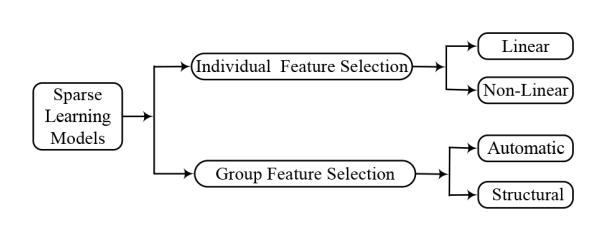
\includegraphics{figure/fig1.png}%
%\caption{.}
%\label{fig:1}
%\end{center}
%\end{figure}

\subsubsection{Linear model}
Consider a linear regression model $\boldsymbol{y}=X\boldsymbol{\beta}+\epsilon$, where $\epsilon=(\epsilon_1,\ldots,\epsilon_n)\sim N(0,\sigma^2I_n)$ is the error vector in which all errors are independent and identically distributed random
variables with zero mean and $\sigma^2$ variance. $\boldsymbol{y}$ is predicted by $\hat{\boldsymbol{y}}=X\hat{\boldsymbol{\beta}}=\sum_{j=1}^{p}\hat{\beta}_{j}\boldsymbol{x}_{(j)}$. $\hat{\boldsymbol{\beta}}=(\hat{\boldsymbol{\beta}}_{1},\ldots,\hat{\beta}_{p})^{T}$ is the estimated coefficient vector obtained by (\ref{eq1}).

\textbf{Lasso}: Lasso proposed by Tibshirani with the $\ell_1$-norm regularization formulation as shown in
\begin{equation}
\hat{\beta}(Lasso)=\underset{\beta\in R^p}{\operatorname{arg}\min}\bigg\{\frac{1}{2}\|\mathbf{y}-X\beta\|_2^2+\lambda\|\beta\|_1\bigg\}
\end{equation}

\textbf{Smoothly Clipped Absolute Deviation (SCAD) Penalty}: Lasso tends to select variables with large coefficients
which may lead to produce biased solutions. The SCAD-based regularizer which reduces bias and yields continuous solutions using the penalty term $\sum_{j=1}^p\mathcal{P}_\lambda(\beta_j)$. $\mathcal{P}_\lambda(\beta_j)$ is a SCAD penalty. Given $a > 2$ and $\lambda \ge 0$, $\mathcal{P}_\lambda(\beta_j)$ is defined as 
\begin{equation}
\mathcal{P}_{\lambda}\big(\beta_{j}\big)=\begin{cases}\lambda|\beta_{j}|,&\text{if}\  |\beta_{j}|\leq\lambda\\ \frac{-|\beta_{j}|^{2}+2a\lambda|\beta_{j}|-\lambda^{2}}{2(a-1)},&\text{if}\  \lambda<|\beta_{j}|\leq a\lambda\\ \frac{(a+1)\lambda^{2}}{2}, &\text{if}\  |\beta_{j}|\geq a\lambda.\end{cases}
\end{equation}
This penalty is a quadratic spline function with knots at $\lambda$ and $a\lambda$.

\textbf{Adaptive Lasso}: By adapting the Lasso penalty term, an adaptive Lasso model was proposed. The adaptive Lasso penalty is a weighted Lasso penalty term as $ \lambda\sum_{j=1}^p\hat{w}_j|\beta_j|$. $\hat{w}_j = 1/|\hat{\beta}_j^{ols}|^\gamma(\gamma>0)$ is the weight of the $j$th coefficient $\beta_j$. $\beta_{j}^{ols}$ is obtained by the ordinary least-square estimation. Compared to Lasso, the adaptive Lasso selects features adaptively by weighting different coefficients.

\textbf{Relaxed Lasso}: 

\textbf{Dantzig Selector (DS)}:

\textbf{Least Absolute Deviation-Lasso (LAD-Lasso)}:

\textbf{Minimax Concave Penalty (MCP)}: 

\textbf{Square-Root Lasso (SRL)}:

\textbf{Uncorrelated Lasso (ULasso)}:

The main advantages of individual linear sparse models lie in: 1) feature selection and parameter estimation are conducted simultaneously and 2) computation is feasible for the feature selection in high-dimensional settings. The disadvantages of these models are: 1) penalties and correlations among features are independent which always leads to unsatisfactory selection results, especially when $p\gg n$  and 2) the correlation structure between features cannot be exploited.


\subsubsection{Nonlinear Models}
Compared to linear regression models, the loss term of nonlinear models is a nonlinear function. The first type of these
functions by introducing the kernel function with the nonlinear response variable being expressed by: $y=\beta_0+\sum_{j=1}^p\beta_j\pmb\phi(\textbf{x}_{(j)})$, $\pmb\phi(\cdot)$ is a (nonlinear) function of the original data $X$ with higher order terms and interactions. To obtain $\hat{\boldsymbol{\beta}}$, the nonlinear function is transformed by
piecewise polynomials, splines, or kernels. In addition, a nonlinear response variable can be transformed into a generalized
linear model by introducing a link function $g(\cdot)$ as follows: $g(E(\mathbf{y}|\mathbf{x}))=\beta_{0}+\sum_{j=1}^{p}\beta_{j}\mathbf{x}_{(j)}$.

\textbf{Featurewise Kernelized Lasso (FWKL)}: Kernel functions are usually introduced to solve nonlinear problems.
To achieve sparsity in terms of features, the FWKL model was presented in \cite{ref3}. A feature-wise procedure rather than an instance-wise way is used for nonlinear transformation which transforms the feature vector $\mathbf{x}_{(j)}$ and the output vector y into a nonlinear function $\pmb\phi(\cdot)$. The FWKL can be expressed by 
\begin{equation}
\boldsymbol{\beta}=\operatorname{arg}\operatorname*{min}_{\boldsymbol{\beta}\in R^{p}}\{\frac{1}{2}\|\boldsymbol{\phi}(y)-\sum_{j=1}^{p}\beta_{j}\boldsymbol{\phi}(\boldsymbol{x}_{(j)})\|_{2}^{2}+\lambda\|\boldsymbol{\beta}\|_1\}
\label{fwkl}
\end{equation}
By using the kernel trick, Eq.(\ref{fwkl}) was shown to be equivalently expressed as the following quadratic programming (QP) problem:
\begin{equation}
\begin{aligned}
\operatorname*{min}_{\boldsymbol\beta\in R^{p}}&\frac{1}{2}\boldsymbol\beta^{T}D\boldsymbol\beta \\
&|{\boldsymbol{\beta}}^{T}d_{(j)}-D(\boldsymbol{x}_{(j)},\boldsymbol{y})|\le\frac{\lambda}{2}, \forall j;
\end{aligned}
\end{equation}
where $D_{j,l}=\pmb{\phi}(\pmb{x}_{(j)})^{T}\pmb{\phi}(\pmb{x}_{(l)}){=}D(\pmb{x}_{(j)},{\pmb{x}}_{(l)})$ and $D=[d_{(1)},\ldots,d_{(p)}]$. This model is also called feature vector machine (FVM), which was extended from the fast grafting algorithm with more general kernels.

\textbf{ Sparse Additive Model (SpAM)}: The SpAM optimization problem can be expressed as
\begin{equation}
\min\limits_{\boldsymbol{\beta}_1,\dots,\boldsymbol{\beta}_d\in\mathbb{R}^n}\|\boldsymbol{y}-\sum\limits_{k=1}^d\boldsymbol{K}^{(k)}\boldsymbol{\beta}_k\|_2^2+\lambda\sum\limits_{k=1}^d\sqrt{\frac{1}{n}\|\boldsymbol{K}^{(k)}\boldsymbol{\beta}_k\|_2^2},
\end{equation}
where $\beta_k = [\beta_{k,1},\ldots,\beta_{k,n}]^\top,k = 1,\ldots,d$ are regression coefficient vectors, $\beta_{k,j}$ is a coefficient for $[K(x_{k,1},x_{k,j}),\ldots,K(x_{k,n},x_{k,j})]^{\top}$, and $\lambda>0 $ is a regularization parameter. An advantage of SpAM is that it is a convex method and can be efficiently optimized by the backfitting algorithm. The potential weakness of SpAM lie in: (a)
it handles only additive models and is ineffective to nonadditive models and (b) SpAM optimization is usually
computationally expensive
\section{基于相似性的特征选择方法}
基于相似性的特征选择方法基于特征保持数据相似性的能力来评估特征的重要性,并通过贪婪准则选择前$K$个特征作为特征选择的结果。其代表性方法有SPEC,Fisher得分,迹比准则等。然而,上述方法往往局限于分类问题,其无法针对回归问题进行特征选择。Laplacian得分作为一种基于相似性的无监督方法,其将保持数据流形结构的能力作为特征的评估标准。其包含三个阶段:首先,构建一个具有$n$个节点的近邻图$\mathcal{G}$,其中的每个节点对应于一个样本;若样本$\bm{x}_i$与$\bm{x}_j$互为近邻,则节点$i$与$j$在近邻图$\mathcal{G}$中相连。然后,计算亲和矩阵(affinity matrix) $\bm{S}$,当节点$i$与$j$相连时,$\bm{S}\left( i,j \right) =\exp \left( -\frac{\left\| \boldsymbol{x}_i-\boldsymbol{x}_j \right\| ^2}{t} \right) $,其中$t$为常数;否则$\bm{S}\left( i,j \right)  = 0$。对角矩阵$\bm{D}$定义为$\bm{D}\left( i,j \right) =\sum\nolimits_{j=1}^n{\bm{S}\left( i,j \right)}$,则Laplacian 矩阵$\bm{L} = \bm{D}-\bm{S}$。最后,每个特征$\bm{f}_r$对应的Laplacian得分为:
\begin{equation}
Lap\_score(\bm{f}_r)=\frac{\tilde{\bm{f}}_{r}^{T}\bm{L}\tilde{\bm{f}}_r}{\tilde{\bm{f}}_{r}^{T}\bm{D}\tilde{\bm{f}}_r}
\end{equation}
其中,$\tilde{\bm{f}}_r=\bm{f}_r-\frac{\bm{f}_{r}^{T}\bm{D}\bm{1}}{\bm{1}^T\bm{D}\bm{1}}\bm{1}$。由于Laplacian得分单独评估每个特征的重要性,所以选择$K$个特征的任务可以通过挑选最小Laplacian得分的前$K$个特征来解决。
Filter类方法采用特定准则如拉普拉斯得分、PCA得分、Pearson相关系数等来对每个特征进行打分,根据得分来对特征进行降序排序,并选择前$K$个特征作为特征选择的结果。Filter类方法原理简单,可以高效地筛选特征,但由于其并未考虑所选特征与建模算法之间的关系,所选特征子集可能并不能在建模算法上取得较好的性能。以数据集$\left\{ \boldsymbol{x}_i,y_i \right\} _{i=1}^{n}$为例,其数据矩阵$X=\left[ \bm{f}_1,\bm{f}_2,\cdots ,\bm{f}_d \right] \in \mathbb{R} ^{n\times d}$,$\bm{f}_r$表示第$r$个特征的值向量;输出变量的值向量为$\bm{y}=\left[ y_1,y_2,\cdots ,y_n \right]^T $。本文对现有主要的特征打分算法进行介绍。
\subsection{Pearson相关系数}
Pearson相关系数的定义如下:
\begin{equation}
R\left( r \right) =\frac{cov\left( \bm{f}_r,\boldsymbol{y} \right)}{\sqrt{var\left( \bm{f}_r \right) \cdot var\left( \boldsymbol{y} \right)}}
\end{equation}
其中,$cov\left( \cdot ,\cdot \right) $表示变量之间的协方差,$var(\cdot)$ 表示变量方差。可以看出,Pearson相关系数仅依据线性关系来对特征进行打分和评价。
\subsection{Laplacian得分}
Laplacian 得分是一种无监督特征选择算法,它选择最能保持数据流形结构的特征。其包含三个阶段:首先,构建一个具有$n$个节点的近邻图$\mathcal{G}$,其中的每个节点对应于一个样本;若样本$\bm{x}_i$与$\bm{x}_j$互为近邻,则节点$i$与$j$在近邻图$\mathcal{G}$中相连。然后,计算亲和矩阵(affinity matrix) $\bm{S}$,当节点$i$与$j$相连时,$\bm{S}\left( i,j \right) =\exp \left( -\frac{\left\| \boldsymbol{x}_i-\boldsymbol{x}_j \right\| ^2}{t} \right) $,其中$t$为常数;否则$\bm{S}\left( i,j \right)  = 0$。对角矩阵$\bm{D}$定义为$\bm{D}\left( i,j \right) =\sum\nolimits_{j=1}^n{\bm{S}\left( i,j \right)}$,则Laplacian 矩阵$\bm{L} = \bm{D}-\bm{S}$。最后,每个特征$\bm{f}_r$对应的Laplacian得分为:
\begin{equation}
Lap\_score(\bm{f}_r)=\frac{\tilde{\bm{f}}_{r}^{T}\bm{L}\tilde{\bm{f}}_r}{\tilde{\bm{f}}_{r}^{T}\bm{D}\tilde{\bm{f}}_r}
\end{equation}
其中,$\tilde{\bm{f}}_r=\bm{f}_r-\frac{\bm{f}_{r}^{T}\bm{D}\bm{1}}{\bm{1}^T\bm{D}\bm{1}}\bm{1}$。由于Laplacian得分单独评估每个特征的重要性,所以选择$K$个特征的任务可以通过挑选最小Laplacian得分的前$K$个特征来解决。
%\subsubsection{SPES}
\subsection{PCA得分}
PCA得分是一种最简单的评价准则,其将特征的方差作为衡量特征重要性的标准,第$r$个特征的PCA得分计算公式为
\begin{equation}
PCA\left( r \right) =\frac{1}{n}\sum_{i=1}^n{\left( x_{i,r}-\mu _r \right) ^2}
\end{equation}
其中,$\mu _r=\frac{1}{n}\sum_{i=1}^n{x_{i,r}}$。PCA得分的大小反映了特征的表示能力,得分值越大说明特征的表示能力越强,其特征重要程度也越大。
\subsection{基于信息度量的Filter方法}
基于信息度量的Filter方法主要是通过设计不同信息准则来对特征的重要性进行度量。该类方法主要针对离散型变量,当变量为连续型时,需要通过一定的离散化技术来对变量进行处理。
首先,给出特征变量的熵、条件熵、互信息以及条件互信息的相关定义。离散型随机变量$X$的熵(Entropy)定义如下:
\begin{equation}
H\left( X \right) =-\sum_{x_i\in X}^{}{P\left( x_i \right) \log \left( P\left( x_i \right) \right)},
\end{equation}
其中,$x_i$表示随机变量$X$的特定值,$p\left(x_i\right)$表示随机变量$X$在特定值$x_i$上的估计概率。 给定另一离散型随机变量$Y$时$X$的条件熵(Conditional Entropy)为
\begin{equation}
H\left( X\left| Y \right. \right) =\sum_{y_j\in Y}{p\left( y_j \right)}\sum_{x_i\in X}^{}{P\left( x_i\left| y_j \right. \right) \log \left( P\left( x_i\left| y_j \right. \right) \right)},
\end{equation}
其中,$p\left( y_j \right)$是$y_j$的先验概率,$P\left( x_i\left| y_j \right. \right)$是$x_i$在$y_j$下的条件概率。条件熵的度量表示给定另一个离散型随机变量$Y$时$X$的不确定性。$X$与$Y$之间的互信息衡量的是$X$与$Y$之间共享的信息量,其计算方式为:
\begin{equation}
\begin{aligned}
I\left( X;Y \right)& =H\left( X \right) -H\left( X\left| Y \right. \right) \\
&=\sum_{x_i\in X}{\sum_{y_j\in Y}{P\left( x_i,y_j \right) \log \frac{P\left( x_i,y_j \right)}{P\left( x_i \right) P\left( y_j \right)},}}
\end{aligned}
\end{equation}
其中,$P\left( x_i,y_j \right)$为$x_i$和$y_j$的联合概率。易知$I\left( X;Y \right)$满足对称性,若$X$与$Y$相互独立,则$I\left( X;Y \right)=0$。与熵的概念类似,在给定第三个离散变量$Z$时,$X$与$Y$之间的条件互信息为:
\begin{equation}
\begin{aligned}
I\left( X;Y\left| Z \right. \right)&=H\left( X\left| Z \right. \right) -H\left( X\left| Y,Z \right. \right) \\
&=\sum_{z_k\in Z}{P\left( z_k \right)}\sum_{x_i\in X}{\sum_{y_j\in Y}{P\left( x_i,y_j\left| z_k \right. \right) \log \frac{P\left( x_i,y_j\left| z_k \right. \right)}{P\left( x_i\left| z_k \right. \right) P\left( y_j\left| z_k \right. \right)}.}}
\end{aligned}
\end{equation}
其表示在随机变量$Z$给定时,$X$与$Y$共享的互信息量。
互信息最大化(Mutual Information Maximization, MIM)通过特征与标签之间的相关性来度量特征的重要性。则特征$x_k$的互信息得分为:
\begin{equation}
J_{MIM}\left( X_k \right) =I\left( X_k;Y \right).
\end{equation}
显然,MIM并未考虑特征之间冗余关系。在得到所有未选特征的MIM特征得分后,选择特征得分最高的特征并将其添加到所选特征集合中,直到获得所需数目的特征子集。
互信息特征选择(Mutual Information Feature Selection, MIFS) 同时考虑特征相关性与冗余性,其特征得分为:
\begin{equation}
J_{MIFS}(X_k)=I(X_k;Y)-\beta\sum_{X_j\in\mathcal{S}}I(X_k;X_j).
\end{equation}
其中,$\mathcal{S}$为所有特征组成的集合。在MIFS中,新特征的特征相关性由第一项$I(X_k;Y)$来评估,而第二项试图惩罚与当前选定特征具有高互信息的特征,以使特征冗余最小化。
最小冗余最大相关(minimum Redundancy Maximum Relevance, mRMR) 基于MIFS方法,将$\beta$设定为选择特征数的倒数,其特征得分为:
\begin{equation}
J_{mRMR}(X_k)=I(X_k;Y)-\frac{1}{|\mathcal{S}|}\sum_{X_j\in\mathcal{S}}I(X_k;X_j).
\end{equation}
显然,MRMR会随着选择特征的增多,逐渐减少特征冗余对得分的影响。基于条件信息熵最大化特征选择(Conditional Infomax Feature Extraction, CIFE) 引入了类-相关冗余的概念来反映类相关性和冗余的复合效应。CIFE通过忽略高阶交互来降低计算复杂性。其对应的表达式为:
\begin{equation}
J_{CIFE}(X_k)=I(X_k;Y)-\sum_{X_j\in\mathcal{S}}I(X_j;X_k)+\sum_{X_j\in\mathcal{S}}I(X_j;X_k|Y).
\end{equation}
其中,第三项用以最大化类相关的冗余性。联合互信息(Joint Mutual Information, JMI)被提出来增加在给定类标签下新特征和已选择特征之间共享的互补信息,其特征得分的计算公式为:
\begin{equation}
J_{JMI}(X_k)=\sum_{X_j\in\mathcal{S}}I(X_k,X_j;Y).
\end{equation}

条件互信息最大化(Conditional Mutual Information Maximization, CMIM)是一种迭代选择特征的准则,该准则在给定所选特征的情况下,使特征与标签的互信息最大化。其特征得分的计算公式为:
\begin{equation}
J_{CMIM}(X_k)=\min_{X_j\in\mathcal{S}}[I(X_k;Y|X_j)].
\end{equation}
式中,通过选择使$I(X_k;Y|X_j)$最小值最大化的特征,可以保证所选特征具有较强的预测能力,并减少对所选特征的冗余。

综上所述, 不同Filter方法的特点如表\ref{tab:4.1}所示。

\begin{table}[htb]
 \begin{center}
 \begin{minipage}[!]{1\linewidth} % 如果想在表格中使用脚注,minipage是个不错的办法
 \caption[Filter类特征选择方法]{不同Filter类特征选择方法对比}
 \label{tab:4.1}
   \begin{tabular*}{\linewidth}{m{2cm}<{\centering}m{7cm}<{\centering}m{2.5cm}<{\centering}m{4cm}<{\centering}} %{\linewidth}{l<{\centering}p{8cm}<{\centering}c<{\centering}c<{\centering}}
     \toprule[1.5pt]
     { 方法名称} & {特征得分} &  {特点} &  {不足} \\
     \midrule[1pt]
     Pearson相关系数 & $cov\left( \bm{f}_r,\boldsymbol{y} \right)\Big/\sqrt{var\left( \bm{f}_r \right) \cdot var\left( \boldsymbol{y} \right)}$ & 基于线性关系 & 未考虑非线性关系 \\
     Laplacian得分 &$\tilde{\bm{f}}_{r}^{T}\bm{L}\tilde{\bm{f}}_r\Big/\tilde{\bm{f}}_{r}^{T}\bm{D}\tilde{\bm{f}}_r$ & 基于样本局部结构 & 未考虑标签信息\\
     PCA得分 &$\frac{1}{n}\sum_{i=1}^n{\left( x_{i,r}-\mu _r \right) ^2}$ & 基于特征方差 & 未考虑标签信息\\
     MIN & $J_{MIM}\left( X_k \right) =I\left( X_k;Y \right)$  & 基于信息度量 & 仅适用于离散型变量\\
	MIFS & $J_{MIFS}(X_k)=I(X_k;Y)-\beta\sum_{X_j\in\mathcal{S}}I(X_k;X_j)$  & 基于信息度量 & 仅适用于离散型变量\\
     mRMR& $J_{MRMR}(X_k)=I(X_k;Y)-\frac{1}{|\mathcal{S}|}\sum_{X_j\in\mathcal{S}}I(X_k;X_j)$  & 基于信息度量 & 仅适用于离散型变量\\
	CIFE & $J_{CIFE}(X_k)=I(X_k;Y)-\sum_{X_j\in\mathcal{S}}I(X_j;X_k)+\sum_{X_j\in\mathcal{S}}I(X_j;X_k|Y)$  & 基于信息度量 & 仅适用于离散型变量\\
      JMI& $J_{JMI}(X_k)=\sum_{X_j\in\mathcal{S}}I(X_k,X_j;Y)$  & 基于信息度量 & 仅适用于离散型变量\\
	CMIM & $J_{CMIM}(X_k)=\min_{X_j\in\mathcal{S}}[I(X_k;Y|X_j)]$  & 基于信息度量 & 仅适用于离散型变量\\
     \bottomrule[1.5pt]
   \end{tabular*}
 \end{minipage}
 \end{center}
\end{table}






\mainmatter
\partsimage{1675670753831.jpg}
\part{聚类模型}
\chapterimage{figure/wallhaven-9d6g28.jpg}

\chapter{聚类模型}
\begin{center}
    \pgfornament[width=0.36\linewidth,color=lsp]{88}
\end{center}
\section{超图}
超图是图论中的一种扩展形式,用以处理和建模复杂的数据相关性。超图在由节点和边组成的传统图模型基础上,进一步引入了超边的概念。传统图模型中的边只能连接两个定点,而超边则可以连接超图中的任意多个顶点,这使得超图在表示和建模复杂结构时具有更好的灵活性和适应性\cite{9264674}。

超图可表示为$\mathcal{G}=\left(\mathcal{V},\mathcal{E}\right)$, 其由一系列的顶点$\mathcal{V}$(vertice)与超边$\mathcal{E} $(hyperedge)组成。在加权超图中,每个超边$e\in\mathcal{E}$都会赋予相应的权重$w(e)$,其表示该连接关系在整个超图中的重要性。则可以通过对角矩阵$\mathbf{W}$表示超图中的超边权重信息,如$\operatorname{diag}(\mathbf{W})=[w(e_1),w(e_2),\ldots,w(e_{|\mathcal{E}|})]$,则加权超图可记为$\mathcal{G}=\left(\mathcal{V},\mathcal{E},\mathbf{W}\right)$,其结构可以通过一个关联矩阵(incidence matrix)$\mathbf{H}\in\{0,1\}^{|\mathcal{V}|\times|\mathcal{E}|}$,其中元素$\mathbf{H}(v,e)$ 表示顶点$v$是否在超边$e$中:
\begin{equation}
\mathbf{H}(v,e)=\left\{\begin{array}{cc}1&\quad\text{if}\quad v\in e\\0&\quad\text{if}\quad v\notin e\end{array}\right.
\end{equation}

在某些情形下,关联矩阵可能并不仅是一个(0,1)-矩阵,而是元素处于0-1区间的连续型矩阵。$\mathbf{H}(v,e)$则表示顶点$v$赋给超边$e$的概率值或顶点$v$对超边$e$的重要性。可定义超边$e$与顶点$v$的重要度分别为
\begin{equation}
\delta(e)=\sum_{v\in\mathcal{V}}\mathbf{H}(v,e)
\end{equation}
\begin{equation}
d(v)=\sum_{e\in\mathcal{E}}w(e)*\mathbf{H}(v,e).
\end{equation}
其对应的对角矩阵分别为$\mathbf{D}_e\in\mathbb{R}^{|\mathcal{E}|*|\mathcal{E}|}$与$\mathbf{D}_v\in\mathbb{R}^{|\mathcal{V}|*|\mathcal{V}|}$。传统图模型的Laplacian矩阵定义为$\mathbf{L} = \mathbf{D}-\mathbf{A}$,其中$\mathbf{D}$为顶点重要度对应的对角矩阵,$\mathbf{A}$为邻接矩阵。
对超图而言其Laplacian矩阵的定义为
\begin{equation}
\mathbf{L}=\mathbf{D}_v-\mathbf{H}\mathbf{W}\mathbf{D}_e^{-1}\mathbf{H}^T.
\end{equation}
Laplacian矩阵标准化后的形式为
\begin{equation}
\mathbf{L}=\mathbf{I}-\mathbf{D}_v^{-1/2}\mathbf{H}\mathbf{W}\mathbf{D}_e^{-1}\mathbf{H}^T\mathbf{D}_v^{-1/2}.
\end{equation}




\section{$k$-means}
给定数据集$\bm{X} = [\bm{x}_1,\bm{x}_2,\cdots,\bm{x}_n]\in\mathbb{R}^{d\times n}$, 并将其划分至$c$个互斥的类别簇$\left\{\mathcal{C}_1,\mathcal{C}_2,\cdots,\mathcal{C}_c\right\}$中. $k$means算法的目标策略是最小化类内误差, 即每个样本点$\bm{x}_i$与其所属簇中心点$\bm{u}_j$之间的欧式距离之和最小, $k$-means的目标函数可写成
\begin{equation}
\begin{aligned}
&\min_{\boldsymbol{Z},\boldsymbol{U}} \left\| \boldsymbol{X}-\boldsymbol{UZ}^T \right\| _{2}^{2}\\
&\mathrm{s}.\mathrm{t}. z_{ij}=\left\{ 0,1 \right\} ,\sum_{j=1}^c{z_{ij}=1,\forall i=1,2,\cdots ,n,}
\end{aligned}
\end{equation}
其中, $\bm{U}\in\mathbb{R}^{d\times c}$ 为簇质心矩阵, $\bm{Z}\in\mathbb{R}^{n\times c}$为簇指示矩阵. 
\subsection{Robust $k$-means}
考虑$k$-means算法聚类性能易受异常点或离群点的影响, 一种鲁棒$k$-均值聚类被提出,
\begin{equation}
\begin{aligned}
&\min_{\bm{Z},\bm{U}}\left\|\bm{X}^T-\bm{ZU}^T\right\|_{2,1}=\sum_{i=1}^n\sqrt{\sum_{j=1}^cz_{ij}||\boldsymbol{x}_i-\boldsymbol{u}_j||^2}\\
&\text{s.t.}\quad z_{ij}=\{0,1\},\sum_{j=1}^cz_{ij}=1,\forall i=1,2,\cdots,n,
\end{aligned}\label{rkmeans}
\end{equation}
式\eqref{rkmeans}通过$\ell_{2,1}$-group正则化来度量重构误差, 通过行稀疏来减少离群点的影响. 其中, $\ell_1$正则化被施加在所有数据点上, $\ell_2$正则化则用于特征上. 

\subsection{Kernel $k$-means}
核化后的$k$-means目标函数为:
\begin{equation}
\begin{aligned}
&\min_{\bm{Z},\bm{V}}\left\|\bm{X}^T-\bm{ZV}^T\right\|_{2}^{2} =\sum_{i=1}^n{\sum_{j=1}^cz_{ij}\left\|\phi(\boldsymbol{x}_i)-\boldsymbol{v}_j\right\|_2^2}\\
&\mathrm{s}.\mathrm{t}. z_{ij}=\left\{ 0,1 \right\} ,\sum_{j=1}^c{z_{ij}=1,\forall i=1,2,\cdots ,n,}
\end{aligned}\label{kkmeans}
\end{equation}
其中, $\phi : \mathbb{R}^d\rightarrow \mathcal{H}$ 为从原始空间到再生核希尔伯特空间的映射函数, 其对应的核函数$\mathcal{K}(\bm{x},\bm{z}) = \phi(\bm{x})^T\phi(\bm{z})$, 且$\phi(\bm{X}) = [\phi(\bm{x}_1),\phi(\bm{x}_2),\cdots,{\phi}(\bm{x}_n)]$. 
由于簇类中心$\bm{v}_j$可以通过映射函数线性表示, 即$\bm{v}_j = \sum_ia_{ij}\phi(\bm{x}_i)$, 其中$a_{ij}$为$\bm{x}_i$属于第$j$簇类的隶属度或概率. 则式\eqref{kkmeans}可以改写为
\begin{equation}
\min\limits_{\bm{Z},\bm{A}}\quad\sum\limits_{i=1}^n{\sum\limits_{j=1}^cz_{ij}(k_{ii}-2\boldsymbol{a}_j^T\boldsymbol{k}_i+\boldsymbol{a}_j^T\bm{K}\boldsymbol{a}_j)},
\end{equation}
其中, $\bm{K}=\phi(\bm{X})^T\phi(\bm{X})\in\mathbb{R}^{n\times n}$, $k_{ii}$为$\bm{K}$在$(i,j)$位置对应的元素, $\bm{k}_i$为$\bm{K}$的第$i$列向量. 采用交替优化算法对式\eqref{kkmeans}进行求解.
\subsubsection{固定\textbf{Z}求解\textbf{V}}
记式\eqref{kkmeans}为$\mathcal{J}(\bm{V})$, 则对$\mathcal{J}(\bm{V})$求$\bm{V}$的偏导可得
\begin{equation}
\frac{\partial \mathcal{J}}{\partial \boldsymbol{v}_j}=-2\sum_{i=1}^n{z_{ij}\left( \phi \left( \boldsymbol{x}_i \right) -\boldsymbol{v}_j \right)}=0
\end{equation}
进一步可得
\begin{equation}
\boldsymbol{v}_j=\frac{\sum_{i=1}^n{z_{ij}\phi \left( \boldsymbol{x}_i \right)}}{\sum_{i=1}^n{z_{ij}}}
\end{equation}
则由$\bm{v}$的定义可知, 矩阵$\bm{A}$中的元素可以通过下式计算得到
\begin{equation}
a_{ij}=\frac{z_{ij}}{\sum_{i=1}^n{z_{ij}}}
\end{equation}
\subsubsection{固定\textbf{V}求解\textbf{Z}}
式\eqref{kkmeans}关于$\bm{Z}$的求解可以分解成求解$n$个独立的子问题, 即
\begin{equation}
\begin{aligned}
&\min_{\boldsymbol{z}_i}\quad{\sum_{j=1}^cz_{ij}({k}_{ii}-2\boldsymbol{a}_j^T{\boldsymbol{k}}_i+\boldsymbol{a}_j^T{\bm{K}}\boldsymbol{a}_j)},\\
&\mathrm{s}.\mathrm{t}. z_{ij}=\left\{ 0,1 \right\} ,\sum_{j=1}^c{z_{ij}=1,\forall i=1,2,\cdots ,n,}
\end{aligned}
\end{equation}
则上述问题的最优解为
\begin{equation}
z_{ij}=\left\{ \begin{array}{l}
	1 \quad j=\mathrm{arg}\min _t\left( \boldsymbol{a}_{t}^{T}\boldsymbol{Ka}_t-2\boldsymbol{a}_{t}^{T}\boldsymbol{k}_{t}^{T} \right)\\
	0  \quad \mathrm{otherwise}.\\
\end{array} \right. 
\end{equation}

\subsection{Robust Kernel $k$-means}
在核$k$-means的基础上进一步对损失函数施加$\ell_{2,1}$正则化约束, 得到如下目标函数:
\begin{equation}
\begin{aligned}
&\min_{\bm{Z},\bm{V}}\left\|\bm{X}^T-\bm{ZV}^T\right\|_{2,1} =\sum_{i=1}^n\sqrt{\sum_{j=1}^cz_{ij}||\phi(\boldsymbol{x}_i)-\boldsymbol{v}_j||^2},\\
&\mathrm{s}.\mathrm{t}. z_{ij}=\left\{ 0,1 \right\} ,\sum_{j=1}^c{z_{ij}=1,\forall i=1,2,\cdots ,n,}
\end{aligned}\label{rkkmeans}
\end{equation}
考虑簇类中心的线性表示$\bm{v}_j = \sum_ia_{ij}\phi(\bm{x}_i)$, 式\eqref{rkkmeans}可进一步改写成:
\begin{equation}
\min\limits_{\bm{Z},\bm{A}}\quad\sum\limits_{i=1}^n\sqrt{\sum\limits_{j=1}^cz_{ij}(k_{ii}-2\boldsymbol{a}_j^T\boldsymbol{k}_i+\boldsymbol{a}_j^T\bm{K}\boldsymbol{a}_j)},
\end{equation}

\subsection{Robust Multiple Kenrel $k$-means}
将多核学习引入至$k$-means 中, 假设有$m$个不同的核函数$\left\{\mathcal{K}\right\}_{t=1}^m$用以聚类任务, 则相应地有$m$个不同的特征空间$\left\{\mathcal{H}\right\}_{t=1}^m$. 为使得组合后的核仍然满足Mercer条件, 构建一个非负特征映射组合$\phi'$, 即
\begin{equation}
\phi'(\boldsymbol{x})=\sum_{t=1}^mw_t\phi_t(\boldsymbol{x})\quad w_t\geq0.
\end{equation}
由于采用线性加权的方式来组合可能会存在维度不匹配的问题, 可构建堆叠所有特征空间

$\tilde{\phi}(\boldsymbol{x})=[\sqrt{w_1}\phi_1(\boldsymbol{x});\sqrt{w_2}\phi_2(\boldsymbol{x});\ldots;\sqrt{w_m}\phi_m(\boldsymbol{x})]^T$构成增广希尔伯特空间$\tilde{\mathcal{H}}=\oplus_{t=1}^m\mathcal{H}^i$, 其与如下组合核函数在特征空间$\tilde{\mathcal{H}}$上等价, 
\begin{equation}
\tilde{\mathcal{K}}(\boldsymbol{x},\boldsymbol{z})=\sum_{t=1}^mw_t\mathcal{K}^t(\boldsymbol{x},\boldsymbol{z}). \label{com_kernel}
\end{equation}
易知式\eqref{com_kernel}中基于$\bm{w}$加权组合的核矩阵仍然保持正定性. 则基于式\eqref{com_kernel}可得
\begin{equation}
\begin{aligned}
\min_{\bm{Z},\bm{A},\boldsymbol{w}}& \sum_{i=1}^n\sqrt{\sum_{j=1}^cz_{ij}[\sum_{t=1}^mw_t(k_{ii}^t-2\boldsymbol{a}_j^T\boldsymbol{k}_i^t+\boldsymbol{a}_j^T\bm{K}^t\boldsymbol{a}_j)]}  \\
&=\sum_{i=1}^n\sqrt{\sum_{j=1}^cz_{ij}(\tilde{k}_{ii}-2\boldsymbol{a}_j^T\tilde{\boldsymbol{k}}_i+\boldsymbol{a}_j^T\bm{\tilde{K}}\boldsymbol{a}_j)}\quad \\
\text{s.t.}& z_{ij}=\{0,1\},\sum_{j=1}^{c}z_{ij}=1,\sum_{t=1}^{m}w_{t}^{\gamma}=1,w_{t}\geq0, 
\end{aligned}
\end{equation}
\section{Isomap}
Isomap作为一种无监督流形学习方法, 其可以用于提取特征. 以数据集$\bm{X}=\left[ \mathbf{x}_1,\cdots,\mathbf{x}_n \right] \in \mathbb{R}^{D\times n}$, $\bm{Y}=\left[ \mathbf{y}_1,\cdots,\mathbf{y}_n \right] \in \mathbb{R}^{d\times n}$, $d\ll D$. 则Isomap的步骤如下:
\begin{enumerate}[1)]
\item 计算所有样本的$k$近邻或$\epsilon$近邻. 
 \item Calculate the geodesic distance $d(\bm{x}_i,\bm{x}_j)$.
 \item  最小化代价函数找到低维表示:
\end{enumerate}



\mainmatter
\partsimage{1675670753831.jpg}
\part{实例选择模型}
\chapterimage{figure/qs2.png}

\chapter{实例选择}
\section{An efficient instance selection algorithm for k nearest neighbor regression}
提出一种适用于MTR问题的原型选择方法(Evolutionary prototype selection for multi-output regression, EPS-MOR),其将训练数据的压缩程度和预测结果的均方误差作为原型选择的评价准则,并采用多目标进化算法NSGA-II来进行寻优。方法在训练阶段基于k-NN算法构建了多目标回归学习器来评估误差,在测试阶段则使用4种不同的MTR模型(Single-target regressor,Multi-target stacking,Regressor chain,Ensemble of regressor chains)来衡量测试误差。通过缓存样本距离矩阵来加速MTR建模的学习效率。采用多目标进化算法时,种群初始化阶段使用不同的概率以及在每个群体中采用不同的进化参数,还使用多个帕累托前沿来防止过拟合,进而得到更加广泛的解方案。

原型选择的第一个目的在于压缩数据集的规模,进而提升模型学习和训练的效率;而第二个目的则是要在压缩数据集上取得较原始数据集相似或更佳的测试性能。(Prototype selection (or instance selection) is one of the tasks at that stage. The first purpose of prototype selection is to obtain a reduced data set that can be used to train predictive models successfully with a similar performance to those that can be obtained using the whole data set.

原型选择试图消除异常、噪声或不适用于学习方法的实例,在进而保证精简后的数据集上仍然可以取得良好的性能表现 .
\section{SMRS}
Sparse Modeling Representative Selection (SMRS)  作为一种过滤型原型选择方法, 其基本思想是通过估计数据的自表达系数, 并从中得到所有样本的相关性得分. 基本假设是每个数据样本都等于或接近原始数据集中某些样本的线性组合. 以数据矩阵$\bm{X}=\left[ \boldsymbol{x}_1,\boldsymbol{x}_2,\cdots ,\boldsymbol{x}_n \right] \in \mathbb{R} ^{d\times n}$为例, 则基于假设可以得到
\begin{equation}
\boldsymbol{x}_i=\boldsymbol{Xa}_i  \quad ( i=1,2,\cdots ,n)
\end{equation}
其中, $\bm{a}_i$为表示样本$\bm{x}_i$的系数或编码向量, 通过整合上式可得$\bm{X}=\bm{XA}$, 其中, $\bm{A} = \left[ \boldsymbol{a}_1,\boldsymbol{a}_2,\cdots ,\boldsymbol{a}_n \right] \in \mathbb{R} ^{n\times n}$. 为了准确有效地估计编码矩阵$\bm{A}$, SMRS构建了如下的目标函数:
\begin{equation}
\min_{\boldsymbol{A}} \left( \frac{1}{2}\left\| \boldsymbol{X}-\boldsymbol{XA} \right\| _{F}^{2}+\lambda \left\| \boldsymbol{A} \right\| _{q,1} \right) \,\,s.t.\mathbf{1}^{\top}\boldsymbol{A}=\boldsymbol{1}^{\top}.
\end{equation}
其中, $q\in\left\{1,2,\infty \right\} $且$\lambda$为非负正则化参数. 通过引入$\ell_{q,1}$正则化, 不仅可以避免产生平凡解, 还可以使得编码矩阵$\bm{A}$产生块稀疏解(如$q=2$时可得到具有行稀疏结构的编码矩阵$\bm{A}$). 因此, 上式给出的优化问题尝试同时在最小重构误差的同时得到具有最少非零行数的编码矩阵, 即以最少数量的具有代表性的样本实现对所有样本的最佳表示. 仿射约束$\mathbf{1}^{\top}\boldsymbol{A}=\boldsymbol{1}^{\top}$ 则维系了全局数据表达的平移不变性, 使目标问题在求解时结果更具鲁棒性. 
 \subsection{Kernelized SMRS}
由于在原始数据空间中, 数据之间的表达性往往难以被察觉或发现, 因此, 传统SMRS在某些具有复杂数据结构的情形下往往难以学习得到准确的数据表达关系. 因此, 引入核技巧将所有原始样本映射至RKHS后, 采用非线性模型来实现数据的自表达性, 不仅使得样本之间的自表示性更具灵活性和适应性, 还可以有效地挖掘样本之间的非线性依赖关系.  因此, 在样本满足非线性分布的情况下, 引入核映射并在RKHS中进行样本的自表示性学习更好的编码矩阵和样本选择结果. 首先, 通过非线性映射$\phi : \bm{x}\rightarrow \phi(\bm{x})$将原始空间中的样本点映射至再生核希尔伯特空间, 则在高维空间中样本矩阵可以表示为 $\varPhi _{\boldsymbol{X}}=\left[ \phi \left( \boldsymbol{x}_1 \right) ,\phi \left( \boldsymbol{x}_2 \right) ,\cdots ,\phi \left( \boldsymbol{x}_n \right) \right] $, 其对应的核函数$\bm{K} (\boldsymbol{x}_i,\boldsymbol{x}_j)=\phi (\boldsymbol{x}_i)^T\phi (\boldsymbol{x}_j)$可以视作样本$\boldsymbol{x}_i$与$\boldsymbol{x}_j$之间的某种相似性度量, 且有 $\bm{K}=\boldsymbol{\varPhi }_{\boldsymbol{X}}^{\top}\boldsymbol{\varPhi }_{\boldsymbol{X}}$. 
则核化后的SMRS的目标函数为
\begin{equation}
\min_{\boldsymbol{A}} \left( \frac{1}{2}\left\| \varPhi _{\boldsymbol{X}}-\varPhi _{\boldsymbol{X}}\boldsymbol{A} \right\| _{F}^{2}+\lambda \left\| \boldsymbol{A} \right\| _{2,1} \right) \,\,s.t. \mathbf{1}^{\top}\boldsymbol{A}=\mathbf{1}^{\top}
\end{equation}
由于仿射约束$\mathbf{1}^{\top}\boldsymbol{A}=\mathbf{1}^{\top}$可以通过将得到的编码矩阵进行列标准化后实现, 且不会影响模型的全局性能, 因此, Kernelized SMRS的目标函数进一步可简化为:
\begin{equation}
\boldsymbol{A}=arg\min_{\boldsymbol{A}}\left( \frac{1}{2}\left\| \varPhi _{\boldsymbol{X}}-\varPhi _{\boldsymbol{X}}\boldsymbol{A} \right\| _{F}^{2}+\lambda \left\| \boldsymbol{A} \right\| _{2,1} \right)
\end{equation}
上式可以通过交替方向乘子优化算法Alternating Direction Method of Multipliers (ADMM)来求解. 

 \subsection{Kernelized SMRS for MTR}
给定MTR样本集$\left\{ \left( \mathbf{x}_i,\mathbf{y}_i \right) \right\} _{i=1}^{n}$, 其中$\bm{x}\in \mathcal{X}$, $\bm{y}\in \mathcal{Y}$. 利用核映射$\phi$将原始的样本输入矩阵$\mathbf{X}=\left[ \mathbf{x}_1,\cdots,\mathbf{x}_n \right]^{T} \in \mathbb{R}^{n\times d}$ 映射至RKHS, 可以构建如下的核SMRS模型:
\begin{equation}
\min_{\boldsymbol{A}} \left( \frac{1}{2}\left\| \varPhi _{\boldsymbol{X}}-\varPhi _{\boldsymbol{X}}\boldsymbol{A} \right\| _{F}^{2}+\lambda \left\| \boldsymbol{A} \right\| _{2,1} \right) \,\,s.t.   \mathbf{1}^{\top}\boldsymbol{A}=\mathbf{1}^{\top}
\end{equation}
相似地, 我们也利用核映射$\varphi $将样本输出矩阵$\mathbf{Y} =\left[ \mathbf{y}_1,\cdots,\mathbf{y}_n\right]^{T}\in \mathbb{R}^{n\times q}$映射至RKHS中, 可构建如下核SMRS模型:
\begin{equation}
\min_{\boldsymbol{B}} \left( \frac{1}{2}\left\| \varPhi _{\boldsymbol{Y}}-\varPhi _{\boldsymbol{Y}}\boldsymbol{B} \right\| _{F}^{2}+\lambda \left\| \boldsymbol{B} \right\| _{2,1} \right) \,\,s.t.   \mathbf{1}^{\top}\boldsymbol{B}=\mathbf{1}^{\top}
\end{equation}
其中, $\bm{B}$为针对目标变量的编码矩阵. 对MTR问题而言, 其在稀疏建模时其特征输入和目标输出上的稀疏建模应当保持相似或一致性, 这样才能更好地进行原型学习, 而这就要求我们学习得到的编码矩阵$\bm{A}$与$\bm{B}$具有相同的稀疏结构. 因此, 我们引入Hilbert-Schmidt独立性准则来度量$\bm{A}$与$\bm{B}$之间的相似性. 


\subsection{Hilbert-Schmidt独立性准则}
Hilbert-Schmidt 独立性准则(Hilbert-Schmidt independence criterion, HSIC)是一种基于核的非参数相关性度量方法, 其通过在再生核希尔伯特空间(Reproducing Kernel Hilbert Space, RKHS)上定义互协方差(Cross-Covariance)算子, 并基于这些算子推导出合适度量独立性的统计量. HSIC通过对Hilbert-Schmidt互协方差算子的经验估计得到独立性判断准则.

考虑一个从可分的度量空间$X$映射至实数空间$\mathbb{R}$的函数对应的可分RKHS为$\mathcal{F}$. 对于点$\boldsymbol{x},\boldsymbol{x'}\in X$, 其在RKHS上的映射$\phi \left( \boldsymbol{x} \right) ,\phi \left( \boldsymbol{x'} \right) \in \mathcal{F}$, 其中$\phi :X\rightarrow \mathcal{F}$为特征映射, 则有$\left< \phi \left( \boldsymbol{x} \right) ,\phi \left( \boldsymbol{x'} \right) \right> _{\mathcal{F}}=k\left( \boldsymbol{x},\boldsymbol{x'} \right) $, 其中$k: X\times X\rightarrow \mathbb{R}$为相关的再生核. 同样定义可分度量空间$Y$对应的RKHS为$\mathcal{G}$, 其具有特征映射$\varphi :Y\rightarrow \mathcal{G}$和相应的再生核$\left< \varphi \left(\boldsymbol{y} \right) ,\varphi \left( \boldsymbol{y'}\right) \right> _{\mathcal{G}}=l\left( \boldsymbol{y},\boldsymbol{y'} \right) $, 其中$\boldsymbol{y},\boldsymbol{y'}\in Y$. 令$\left( \boldsymbol{x,y} \right) $为$X\times Y$上服从联合概率分布或测度$P_{\boldsymbol{x,y}}$的随机变量, 则特征映射$\phi$和$\varphi $之间的互协方差算子可定义为线性算子$C_{\boldsymbol{x},\boldsymbol{y}}:\mathcal{G}\rightarrow \mathcal{F}$: 
\begin{equation}
C_{\boldsymbol{x},\boldsymbol{y}}=E_{\boldsymbol{x},\boldsymbol{y}}\left[ \left[ \phi \left( \boldsymbol{x} \right) -E_{\boldsymbol{x}}\left[ \phi \left( \boldsymbol{x} \right) \right] \right] \otimes \left[ \varphi \left( \boldsymbol{y} \right) -E_{\boldsymbol{y}}\left[ \varphi \left( \boldsymbol{y} \right) \right] \right] \right] 
\end{equation}
其中$\otimes $为张量积或直积; $E_{\boldsymbol{xy}}$,  $E_{\boldsymbol{x}}$和 $E_{\boldsymbol{y}}$分别是关于联合概率$P_{\boldsymbol{x,y}}$, 边缘分布$P_{\boldsymbol{x}}$和$P_{\boldsymbol{y}}$的期望. 则HSIC的定义如下:
\begin{equation}
\begin{aligned}
\text{HSIC}\left( \mathcal{F},\mathcal{G},P_{\boldsymbol{x,y}} \right)  = \lVert C_{\boldsymbol{x,y}} \rVert _{\text{HS}}^{2} = &E_{\boldsymbol{x,x',y,y'}}\left[ k\left( \boldsymbol{x,x'} \right) l\left( \boldsymbol{y,y'} \right) \right] -2E_{\boldsymbol{x,y}}\left[ E_{\boldsymbol{x'}}\left[ k\left( \boldsymbol{x,x'} \right) \right] E_{\boldsymbol{y}}\left[ l\left( \boldsymbol{y,y'} \right) \right] \right] \\
&+E_{\boldsymbol{x,x'}}\left[ k\left( \boldsymbol{x,x'} \right) \right] E_{\boldsymbol{y,y'}}\left[ l\left( \boldsymbol{y,y'} \right) \right] 
\end{aligned}
\end{equation}
其中, $E_{\boldsymbol{x,x',y,y'}}$表示从$P_{\boldsymbol{x,y}}$中独立提取有关$\left( \boldsymbol{x,y} \right)$和$\left( \boldsymbol{x',y'} \right) $的期望值. 不难看出, 当核$k$和$l$有界时,  $C_{\boldsymbol{x,y}}$的Frobenius范数存在. 若两个特征映射$\phi$和$\varphi$均为线性映射, 即$\phi \left( \boldsymbol{x} \right) =\boldsymbol{x}$和$\varphi \left( \boldsymbol{y} \right) =\boldsymbol{y}$, HSIC与互协方差算子$C_{\boldsymbol{x,y}}$的Frobenius范数的平方相同. 

为了更好地对统计独立性进行度量, 需在给定有限个观测样本的情况下对HSIC进行估计. 给定核$k$和$l$以及由联合概率分布$P_{\boldsymbol{x,y}}$得到的一组观测样本$D=\left\{ \left( \boldsymbol{x}_i,\boldsymbol{y}_i \right) \right\} _{i=1}^{N}$, 文献[]提出了具有$O\left( n^{-1} \right) $偏差的HSIC估计量, 用以对其进行近似估计, 其表示为
\begin{equation}
\text{HSIC}_0\left( \mathcal{F},\mathcal{G},D \right) =\frac{1}{\left( N-1 \right) ^2}tr\left( \boldsymbol{KHLH} \right) 
\end{equation}
其中, $\boldsymbol{H}=\boldsymbol{I}_N-\boldsymbol{1}_N\boldsymbol{1}_N^{T}/{N}\in \mathbb{R}^{N\times N}$为中心化矩阵, $\boldsymbol{I}$ 为单位矩阵, $\boldsymbol{1}_N$ 为元素全为 1 的 $N$ 维列向量; $\boldsymbol{K},\boldsymbol{L}\in \mathbb{R}^{N\times N}$分别为基于核$k$和$l$构建的Gram矩阵, 其中, $\boldsymbol{K}_{i,j}=k\left( \boldsymbol{x}_i,\boldsymbol{x}_j \right) $ 且 $\boldsymbol{L}_{i,j}=l\left( \boldsymbol{y}_i,\boldsymbol{y}_j \right) $. 
HSIC已用于特征选择, 降维以及聚类等多种学习任务中, 这说明HSIC在度量不同随机变量之间的相关性时具有良好的适用性和鲁棒性, 其不仅可以有效度量线性统计相关性, 还可以检测非线性统计相关性.




\subsection{SMRS with sparse similarity maximization}
基于HSIC构建编码矩阵$\bm{A}$与$\bm{B}$之间的相似性度量, 可表示为
\begin{equation}
    HSIC(\bm{A},\bm{B}) = (n-1)^{-2}tr(\bm{HK}_A\bm{HK}_B)
\end{equation}
其中, $\bm{K}_A = \bm{A}^{\top}\bm{A}$与$\bm{K}_B = \bm{B}^{\top}\bm{B}$ 分别为输入和输出编码矩阵所对应的内积. 为了保证MTR情境中的输入和输出编码矩阵具有最大的结构相似性, 将基于HSIC构建的相似性度量引入至核化SMRS模型中, 得到最终的目标函数为
\begin{equation}
    \begin{aligned}
    \min_{\boldsymbol{A},\boldsymbol{B}} &\frac{1}{2}\left( \left\| \varPhi _{\boldsymbol{X}}-\varPhi _{\boldsymbol{X}}\boldsymbol{A} \right\| _{F}^{2}+\left\| \varPhi _{\boldsymbol{Y}}-\varPhi _{\boldsymbol{Y}}\boldsymbol{B} \right\| _{F}^{2} \right) \\
    &+\lambda \left( \left\| \boldsymbol{A} \right\| _{2,1}+\left\| \boldsymbol{B} \right\| _{2,1} \right) -\alpha tr\left( \boldsymbol{HA}^{\top}\boldsymbol{AHB}^{\top}\boldsymbol{B} \right) \\
    &\,\,s.t.\ 1^{\top}\boldsymbol{A}=1^{\top},\,\,1^{\top}\boldsymbol{B}=1^{\top}
    \end{aligned}\label{smrsssm}
\end{equation}
式中第一项和第二项为针对MTR数据的输入和输出稀疏编码, 第三项则为基于HSIC的稀疏矩阵相似性度量. 

\subsection{基于交替优化乘子算法(ADMM)的求解(不太行)}

由于\eqref{smrsssm}中的仿射约束均可通过对编码矩阵$\bm{A}$和$\bm{B}$的列标准化来满足, 为了更好地基于ADMM算法进行求解, 引入哑变量将其改写为
\begin{equation}
    \begin{aligned}
\min_{\boldsymbol{A},\boldsymbol{B}}&\frac{1}{2}\left( \left\| \varPhi _{\boldsymbol{X}}-\varPhi _{\boldsymbol{X}}\boldsymbol{A} \right\| _{F}^{2}+\left\| \varPhi _{\boldsymbol{Y}}-\varPhi _{\boldsymbol{Y}}\boldsymbol{B} \right\| _{F}^{2} \right) +\,\lambda \left( \left\| \boldsymbol{C} \right\| _{2,1}+\left\| \boldsymbol{D} \right\| _{2,1} \right)\\
& \frac{\rho _1}{2}\left\| \boldsymbol{A}-\boldsymbol{C} \right\| _{F}^{2}+\frac{\rho _2}{2}\left\| \boldsymbol{B}-\boldsymbol{D} \right\| _{F}^{2}-\alpha tr\left( \boldsymbol{HA}^{\top}\boldsymbol{AHB}^{\top}\boldsymbol{B} \right) \\
\,\,&s.t.  \boldsymbol{A}=\boldsymbol{C}, \boldsymbol{B}=\boldsymbol{D}.
\end{aligned}
\end{equation}
则上式的拉格朗日形式为
\begin{equation}
    \begin{aligned}
        L_{\rho _1,\rho _2}\left( \boldsymbol{A},\boldsymbol{B},\boldsymbol{C},\boldsymbol{D},\boldsymbol{\varLambda },\boldsymbol{\varPi } \right) =&\frac{1}{2}\left( \left\| \varPhi _{\boldsymbol{X}}-\varPhi _{\boldsymbol{X}}\boldsymbol{A} \right\| _{F}^{2}+\left\| \varPhi _{\boldsymbol{Y}}-\varPhi _{\boldsymbol{Y}}\boldsymbol{B} \right\| _{F}^{2} \right) +\,\lambda \left( \left\| \boldsymbol{C} \right\| _{2,1}+\left\| \boldsymbol{D} \right\| _{2,1} \right)\\
        & \frac{\rho _1}{2}\left\| \boldsymbol{A}-\boldsymbol{C} \right\| _{F}^{2}+\frac{\rho _2}{2}\left\| \boldsymbol{B}-\boldsymbol{D} \right\| _{F}^{2}-\alpha tr\left( \boldsymbol{HA}^{\top}\boldsymbol{AHB}^{\top}\boldsymbol{B} \right) \\
        & +tr\left( \boldsymbol{\varLambda }^{\top}\left( \boldsymbol{A}-\boldsymbol{C} \right) \right) +tr\left( \boldsymbol{\varPi }^{\top}\left( \boldsymbol{B}-\boldsymbol{D} \right) \right) 
    \end{aligned}
\end{equation}
其中, $\rho_1>0$和$\rho_2>0$. $\boldsymbol{\varLambda}$ 与 $\boldsymbol{\varPi }$ 为拉格朗日乘子矩阵. 则ADMM算法步骤如下:
\begin{enumerate}[1)]
    \item $\boldsymbol{A}_{t+1}=\mathop {arg\min} \limits_{\bm{A}}L_{\rho _1,\rho _2}\left( \boldsymbol{A},\boldsymbol{B}_t,\boldsymbol{C}_t,\boldsymbol{D}_t,\boldsymbol{\varLambda }_t,\boldsymbol{\varPi }_t \right)$. 通过计算$\bm{A}$关于$L_{\rho _1,\rho _2}$的偏导,可得
    \begin{equation}
        \left( \boldsymbol{K}_{\bm{X}}+\rho _1\boldsymbol{I}_n \right) \boldsymbol{A}-\alpha \boldsymbol{AHB}_{t}^{\top}\boldsymbol{B}_t\boldsymbol{H}=\boldsymbol{K}_{\bm{X}}+\rho _1\boldsymbol{C}_t+\boldsymbol{\varLambda }_t
    \end{equation}
    其为标准的Sylvester方程, 可以通过求解方程得到其解析解. 
    \item $\boldsymbol{B}_{t+1}=\mathop {arg\min} \limits_{\bm{B}}L_{\rho _1,\rho _2}\left( \boldsymbol{A}_t,\boldsymbol{B},\boldsymbol{C}_t,\boldsymbol{D}_t,\boldsymbol{\varLambda }_t,\boldsymbol{\varPi }_t \right)$. 通过计算$\bm{B}$关于$L_{\rho _1,\rho _2}$的偏导,可得
    \begin{equation}
        \left( \boldsymbol{K}_{\bm{Y}}+\rho _2\boldsymbol{I}_n \right) \boldsymbol{B}-\beta \boldsymbol{BHA}_{t}^{\top}\boldsymbol{A}_t\boldsymbol{H}=\boldsymbol{K}_{\bm{Y}}+\rho _2\boldsymbol{D}_t+\boldsymbol{\varPi}_t
    \end{equation}
    \item $\boldsymbol{C}_{t+1}=\mathop {arg\min} \limits_{\bm{C}}L_{\rho _1,\rho _2}\left( \boldsymbol{A}_t,\boldsymbol{B}_t,\boldsymbol{C},\boldsymbol{D}_t,\boldsymbol{\varLambda }_t,\boldsymbol{\varPi }_t \right)$. 则可以得到
    \begin{equation}
        \min_{\boldsymbol{C}} \lambda \left\| \boldsymbol{C} \right\| _{1,2}+\frac{\rho _1}{2}\left\| \boldsymbol{A}-\boldsymbol{C} \right\| _{F}^{2}+tr\left( \boldsymbol{\varLambda }^{\top}\left( \boldsymbol{A}-\boldsymbol{C} \right) \right) 
    \end{equation}
    上式可基于下式计算得到:
	 \begin{equation}
        \boldsymbol{C}_{t+1}=\mathcal{S} _{\frac{\lambda}{\rho _1}}\left[ \boldsymbol{A}_{t+1}+\frac{\boldsymbol{\varLambda }_t}{\rho _1} \right] 
    \end{equation}
    其中, 有软阈值算子如下:
    \begin{equation}
    \boldsymbol{Z}^\prime=\mathcal{S} _s\left[ \boldsymbol{Z} \right] =\begin{cases}
        z_{ij}^{\prime}=\frac{r_i-s}{r_i+s}z_{ij},  r_i\geqslant s\\
        0,             \mathrm{otherwise}\\
    \end{cases}\label{eq3.18}
    \end{equation}
    其中, $r_i=\left\| \boldsymbol{Z}_{i\cdot} \right\| _2$.
    \item $\boldsymbol{D}_{t+1}=\mathop {arg\min} \limits_{\bm{D}}L_{\rho _1,\rho _2}\left( \boldsymbol{A}_t,\boldsymbol{B}_t,\boldsymbol{C}_t,\boldsymbol{D},\boldsymbol{\varLambda }_t,\boldsymbol{\varPi }_t \right)$. 则同样可得
    \begin{equation}
        \min_{\boldsymbol{D}} \lambda \left\| \boldsymbol{D} \right\| _{1,2}+\frac{\rho _1}{2}\left\| \boldsymbol{B}-\boldsymbol{D} \right\| _{F}^{2}+tr\left( \boldsymbol{\varLambda }^{\top}\left( \boldsymbol{B}-\boldsymbol{D} \right) \right) 
    \end{equation}
    其同样可基于软阈值算子\eqref{eq3.18}得到解析解:
    \begin{equation}
        \boldsymbol{D}_{t+1}=\mathcal{S} _{\frac{\lambda}{\rho _2}}\left[ \boldsymbol{B}_{t+1}+\frac{\boldsymbol{\varPi }_t}{\rho _2} \right] 
    \end{equation}
    \item $\boldsymbol{\varLambda }_{t+1} = \boldsymbol{\varLambda }_t+\rho_1(\bm{A}_{t+1}-\bm{C}_{t+1})$.
    \item $\boldsymbol{\varPi }_{t+1} = \boldsymbol{\varPi }_t+\rho_1(\bm{B}_{t+1}-\bm{D}_{t+1})$.
\end{enumerate}

\subsection{SMRS在MTR问题中的两种关系假设}
在MTR问题中, 我们认为不能仅基于样本输入之间的表示关系来进行原型学习和样本选择, 样本在目标空间上的标签信息同样应当被考虑. 如图所示, 若在特征空间中, 样本$\bm{x}$与样本子集$\left\{ \bm{x}_i,\bm{x}_j,\bm{x}_k\right\}$之间存在某种表示关系, 即$\bm{x}$可以被$\left\{ \bm{x}_i,\bm{x}_j,\bm{x}_k\right\}$中的样本组合表示. 则我们认为它们对应的输出在目标空间中也存在相似的表示关系, 即$\bm{y}$可以被子集$\left\{ \bm{y}_i,\bm{y}_j,\bm{y}_k\right\}$所表示. 
\begin{figure}
	\begin{center}
	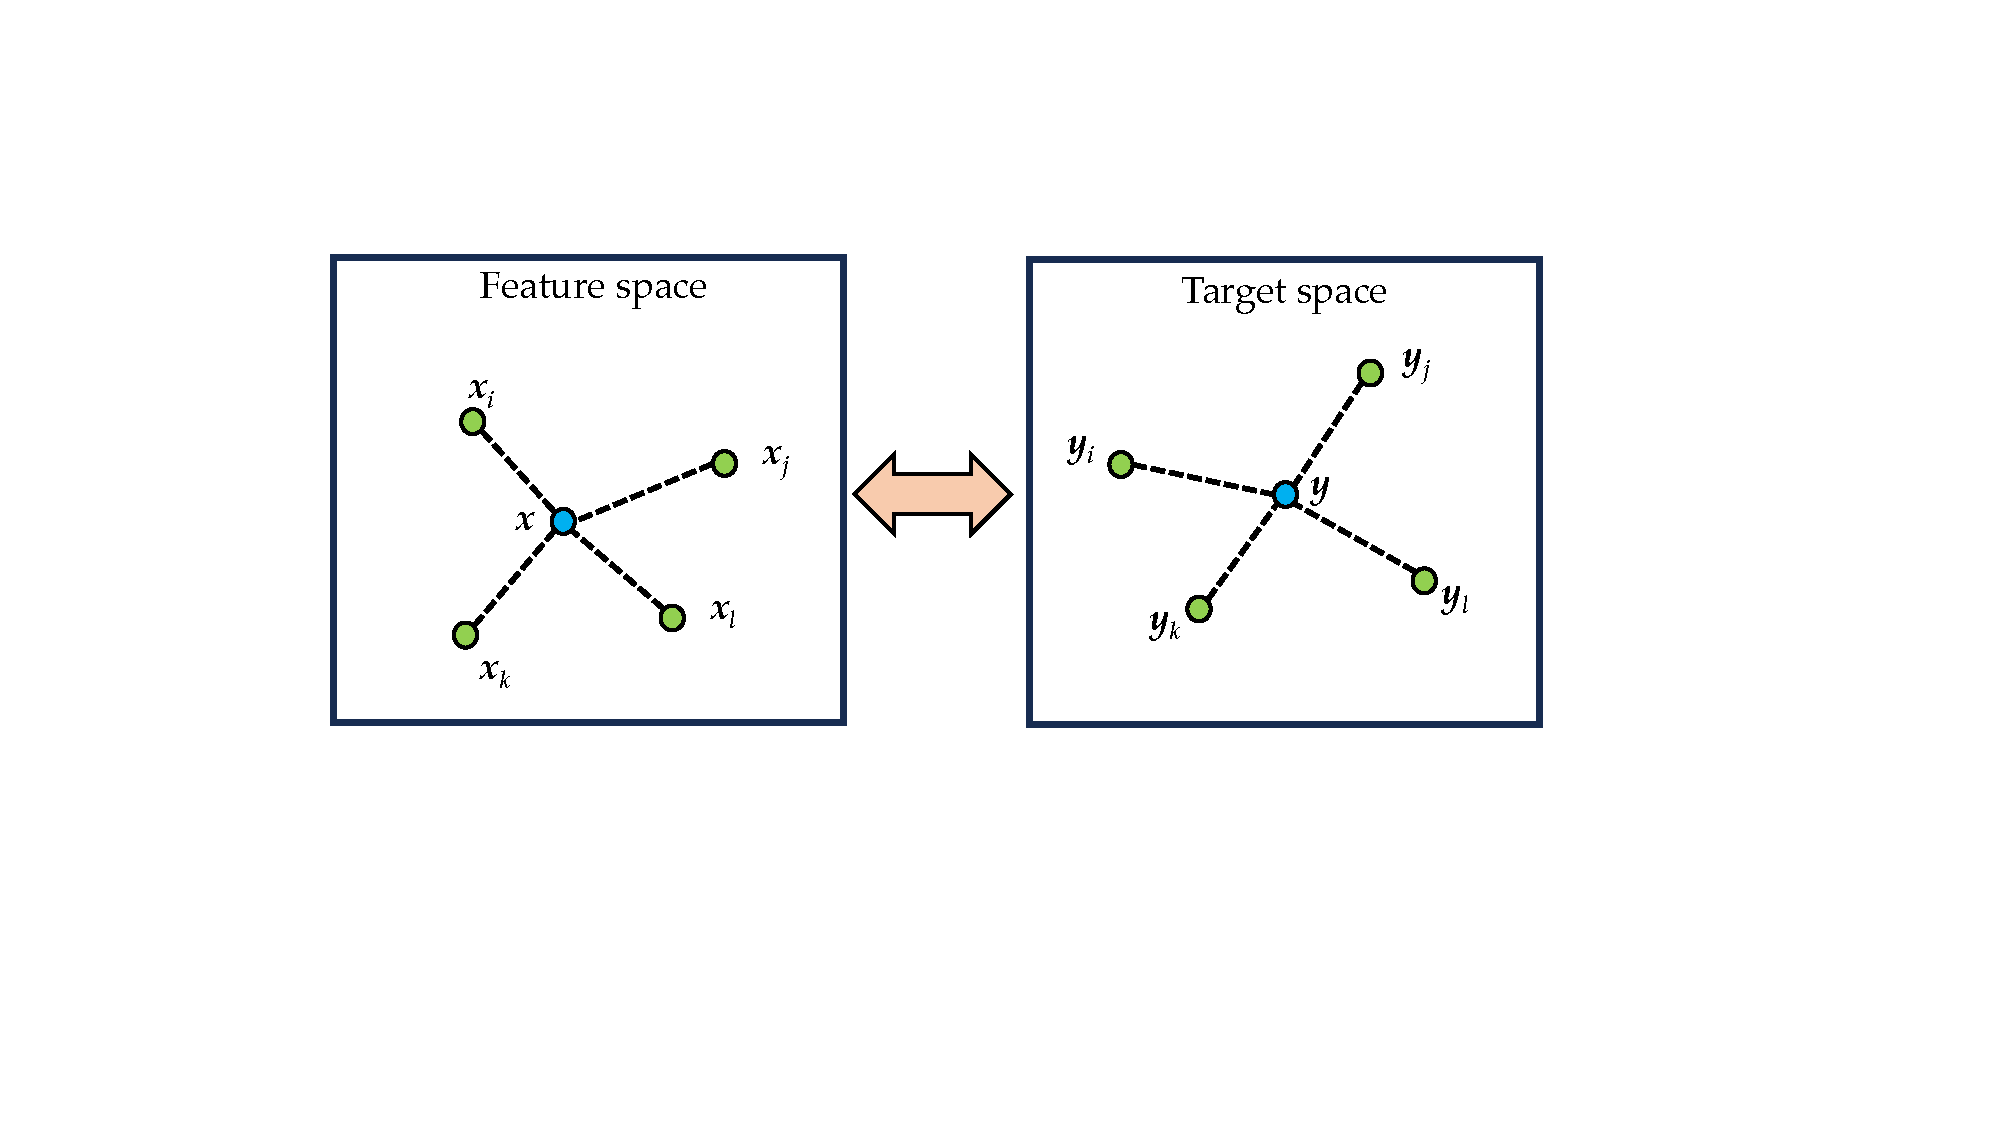
\includegraphics[width=0.99\textwidth]{figure/fig1.pdf}%
	\caption{样本在特征空间与目标空间上具有一致或相似的自表示性.}
	\label{fig1}
\end{center}
\end{figure}
因此, 基于上述假设, 我们构建了基于目标的SMRS模型如下:
\begin{equation}
    \min_{\boldsymbol{B}} \left( \frac{1}{2}\left\| \boldsymbol{Y}-\boldsymbol{YB} \right\| _{F}^{2}+\lambda \left\| \boldsymbol{B} \right\| _{2,1} \right) \,\,s.t.\mathbf{1}^{\top}\boldsymbol{B}=\boldsymbol{1}^{\top}.
\end{equation}
由于不同目标变量之间的潜在关联关系可能导致在目标空间中的自表示关系的探索和挖掘效果不佳, 为了解决该问题, 我们提出了两种策略:
\begin{enumerate}[1)]
    \item 利用样本的目标向量之间的相似关系来替代原始目标变量输出, 即将输出矩阵$\bm{Y}$用相似性矩阵$\bm{S}$替代, 其中$\bm{s}_i = \left[ sim\left( \boldsymbol{y}_i,\boldsymbol{y}_1 \right) ,\cdots ,sim\left( \boldsymbol{y}_i,\boldsymbol{y}_n \right) \right] ^{\top}$, $sim\left(\boldsymbol{y}_i,\boldsymbol{y}_j \right)$ 为目标向量 $\boldsymbol{y}_i$ 与 $\boldsymbol{y}_j$ 之间的相似性度量. 
    \item 利用核映射将目标向量映射至RKHS中进行自表示关系挖掘, 在高维空间中挖掘样本之间潜在的表示关系. 
\end{enumerate}

则基于策略1可构建如下的目标函数
\begin{equation}
    \min_{\boldsymbol{B}} \left( \frac{1}{2}\left\| \boldsymbol{S}-\boldsymbol{SB} \right\| _{F}^{2}+\lambda \left\| \boldsymbol{B} \right\| _{2,1} \right) \,\,s.t. \  \mathbf{1}^{\top}\boldsymbol{B}=\boldsymbol{1}^{\top}.\label{eq3.22}
\end{equation}
其中, 我们采用余弦相似度度量目标向量之间的相似性, 即$sim\left( \boldsymbol{y}_i,\boldsymbol{y}_j \right) =\frac{\left< \boldsymbol{y}_i,\boldsymbol{y}_j \right>}{\left\| \boldsymbol{y}_i \right\| \cdot \left\| \boldsymbol{y}_j \right\|}$.
策略2推广出的目标函数为
\begin{equation}
    \min_{\boldsymbol{B}} \left( \frac{1}{2}\left\| \boldsymbol{\varPhi }_Y-\boldsymbol{\varPhi }_Y\boldsymbol{B} \right\| _{F}^{2}+\lambda \left\| \boldsymbol{B} \right\| _{2,1} \right) \,\,s.t. \  \mathbf{1}^{\top}\boldsymbol{B}=\mathbf{1}^{\top}.\label{eq3.23}
\end{equation}
其中, $\boldsymbol{\varPhi }_Y$ 为基于核函数$\varphi$映射至RKHS的样本矩阵. 通过式\eqref{eq3.22}或\eqref{eq3.23}挖掘不同样本在目标空间上的自表示信息后, 我们引入Hilbert-Schmidt独立性准则来度量特征空间和目标空间在自表示上的相似性, 则可得如下目标函数,
\begin{equation}
    \max_{\boldsymbol{A},\boldsymbol{B}} tr\left( \boldsymbol{HA}^{\top}\boldsymbol{AHB}^{\top}\boldsymbol{B} \right)
\end{equation}
基于上述两种策略, 将其与特征的核化SMRS模型以及基于HSIC的相似性度量项结合后可以得到如下两种目标函数:
\begin{equation}
    \begin{aligned}
        SMRS\_I: \min_{\boldsymbol{A},\boldsymbol{B}}\ \ &\frac{1}{2}\left( \left\| \varPhi _{\boldsymbol{X}}-\varPhi _{\boldsymbol{X}}\boldsymbol{A} \right\| _{F}^{2}+\left\| \varPhi _{\boldsymbol{Y}}-\varPhi _{\boldsymbol{Y}}\boldsymbol{B} \right\| _{F}^{2} \right) \\
        & +\lambda \left( \left\| \boldsymbol{A} \right\| _{2,1}+\left\| \boldsymbol{B} \right\| _{2,1} \right)-\beta tr\left( \boldsymbol{HA}^{\top}\boldsymbol{AHB}^{\top}\boldsymbol{B} \right)\\
        &\,\,s.t.\ \mathbf{1}^{\top}\boldsymbol{A}=\mathbf{1}^{\top},\,\,\mathbf{1}^{\top}\boldsymbol{B}=\mathbf{1}^{\top}
        \end{aligned}
\end{equation}

\begin{equation}
    \begin{aligned}
        SMRS\_II: \min_{\boldsymbol{A},\boldsymbol{B}}\ \ &\frac{1}{2}\left( \left\| \varPhi _{\boldsymbol{X}}-\varPhi _{\boldsymbol{X}}\boldsymbol{A} \right\| _{F}^{2}+\left\| \boldsymbol{S}-\boldsymbol{S}\boldsymbol{B} \right\| _{F}^{2} \right)  \\
        & +\lambda \left( \left\| \boldsymbol{A} \right\| _{2,1}+\left\| \boldsymbol{B} \right\| _{2,1} \right)- \beta tr\left( \boldsymbol{HA}^{\top}\boldsymbol{AHB}^{\top}\boldsymbol{B} \right)\\
        & \,\,s.t.\ \mathbf{1}^{\top}\boldsymbol{A}=\mathbf{1}^{\top},\,\,\mathbf{1}^{\top}\boldsymbol{B}=\mathbf{1}^{\top}
        \end{aligned}
\end{equation}
上式都可通过算法1求解.

% \begin{algorithm}
% \caption{SMRS\_I求解伪代码}}\label{algorithm2}
% \KwIn{input matrix $\bm{X}$, target matrix $\bm{Y}$;}
% \KwOut{encode matrix $bm{A}$ and $\bm{B}$;} 
% 	initialization $\bm{A}$ and $\bm{B}$;\\
% \Repeat(:){converges}{Calculate $\mathbf{U}_{t+1}=\mathbf{D}_{t}^{-1}\mathbf{A}^T\left( \mathbf{AD}_{T}^{-1}\mathbf{A}^T \right) ^{-1}\mathbf{Y.}$\;
% 	Calculate the diagonal matrix $\mathbf{D}_{t+1}$, where the $i$-th diagonal element is $\frac{1}{2\lVert \mathbf{u}_{t+1}^{i} \rVert _2}$\;
% 	$t=t+1$.}
% \end{algorithm}

\subsection{MTR中原型选择模型构建}
通常情况下, MTR问题的输入与输出空间均为多维连续型实值空间, 与多标签分类中的原型选择不同的是, 其并不存在数据类别的概念, 因此也并不存在类边界, 这使得基于边界的原型选择方法在MTR问题中失效. 而基于近邻结构的原型选择算法则忽视了样本中的目标变量信息, 致使所选择的原型集合上不一定能得到较好的回归性能. 最为重要的是, MTR问题中的原型选择应当保证目标变量之间的相关性信息得以保留, 才能使得后续的建模学习中可以更好地通过探索和挖掘目标间的相关关系来提升模型性能. \cite{absil2009optimization}

% \partsimage{1675670753831.jpg}
% \part{参考文献}
\chapterimage{figure/qs2.png}
% \small
\printbibliography
% \bibliography{reference}
% \bibliographystyle{icml2016}

\end{document}
